\NeedsTeXFormat{LaTeX2e}
\documentclass[ngerman,a4paper,pagesize,oneside,headinclude,parskip=half,DIV14,BCOR5mm,12pt,listof=totoc,bibliography=totoc]{scrbook}
\KOMAoptions{DIV=current}

\pagestyle{headings}
\usepackage{ngerman}
%\usepackage[latin1]{inputenc}
%\usepackage[applemac]{inputenc} % Mac-Nutzer
\usepackage[utf8]{inputenc}
\usepackage[T1]{fontenc}
\usepackage{lmodern}
%\renewcommand{\sfdefault}{phv}
%\renewcommand{\rmdefault}{phv}
%\renewcommand{\ttdefault}{pcr}
\usepackage[gen,right]{eurosym}
\usepackage{actuar}
\usepackage[intoc]{nomencl}
\usepackage[printonlyused]{acronym}
\usepackage{graphicx}
\usepackage{verbatim}
\usepackage{tabularx}
\usepackage{booktabs}
\usepackage[table]{xcolor}
\usepackage{url}
\usepackage{color}
\usepackage{amssymb,amsmath}
\usepackage{setspace}
\usepackage{scrhack}
\usepackage{floatrow}
\usepackage{float}
\usepackage{listings}
\usepackage{hyperref}
% Fortlaufende Fußnoten über die gesamte Arbeit 
\usepackage{remreset}
\usepackage{tcolorbox}
\usepackage{array}
\usepackage[section]{placeins}
\usepackage{eurosym}
\usepackage{subfig}
\usepackage{courier}
\makeatletter
\@removefromreset{footnote}{chapter}



\definecolor{lightgray}{rgb}{0.95, 0.95, 0.95}
\definecolor{darkgray}{rgb}{0.4, 0.4, 0.4}
%\definecolor{purple}{rgb}{0.65, 0.12, 0.82}
\definecolor{editorGray}{rgb}{0.95, 0.95, 0.95}
\definecolor{editorOcher}{rgb}{1, 0.5, 0} % #FF7F00 -> rgb(239, 169, 0)
\definecolor{editorGreen}{rgb}{0, 0.5, 0} % #007C00 -> rgb(0, 124, 0)
\definecolor{orange}{rgb}{1,0.45,0.13}		
\definecolor{olive}{rgb}{0.17,0.59,0.20}
\definecolor{brown}{rgb}{0.69,0.31,0.31}
\definecolor{purple}{rgb}{0.38,0.18,0.81}
\definecolor{lightblue}{rgb}{0.1,0.57,0.7}
\definecolor{lightred}{rgb}{1,0.4,0.5}
\usepackage{upquote}
\usepackage{listings}


\makeatother
% hier Namen etc. einsetzen
\newcommand{\titel}{Kombinatorische Testmethoden zur Analyse aktuarieller Software} %siehe Datei 00_title.tex für Generierung der Titelseite
\newcommand{\type}{Bachelorarbeit}
\newcommand{\fullname}{Johannes Gabriel Sindlinger}
\newcommand{\email}{johannes.sindlinger@uni-ulm.de}
\newcommand{\datum}{23.10.2021}
\newcommand{\matnr}{961403}
\newcommand{\gutachterA}{Prof.~Dr.~Manfred Reichert}
\newcommand{\fakultaet}{Ingenieurwissenschaften, Informatik und Psychologie}
\newcommand{\institut}{Institut für Datenbanken und Informationssysteme}
\newcommand{\studiengang}{Informatik}

\newcommand{\N}{\mathbb{N}}
\newcommand{\R}{\mathbb{R}}
\newcommand{\rd}[1]{\mathcal{R}_{#1}}
\newcommand{\rt}[1]{\widehat{\mathcal{R}}_{#1}}
\newcommand{\E}{\mbox{I\negthinspace E}}

\renewcommand{\arraystretch}{1.5}
\newcolumntype{P}[1]{>{\centering\arraybackslash}p{#1}}


%color in tables
\usepackage{colortbl}
\definecolor{Gray}{rgb}{0.80784, 0.86667, 0.90196} %dunkelblau
\definecolor{Lightgray}{rgb}{0.9176, 0.95, 0.95686} %hellblau
\definecolor{Akzent}{rgb}{0.6627, 0.63529, 0.55294} %akzentfarbe

\definecolor{red1}{RGB}{244,130,147} %hellrot
\definecolor{red2}{RGB}{230,53,79} %mittelrot
\definecolor{red3}{RGB}{64,15,22} %dunkelrot
\definecolor{grauinfo}{RGB}{125,154,169}

\definecolor{javared}{rgb}{0.6,0,0} % for strings
\definecolor{javagreen}{rgb}{0.25,0.5,0.35} % comments
\definecolor{javapurple}{rgb}{0.5,0,0.35} % keywords
\definecolor{javadocblue}{rgb}{0.25,0.35,0.75} % javadoc
 
\lstset{language=Java,
basicstyle=\ttfamily,
keywordstyle=\color{red3}\bfseries,
stringstyle=\color{red2},
commentstyle=\color{grauinfo},
morecomment=[s][\color{javadocblue}]{/**}{*/},
numbers=left,
numberstyle=\tiny\color{black},
stepnumber=1,
numbersep=10pt,
tabsize=4,
showspaces=false,
showstringspaces=false}
\setlength{\arrayrulewidth}{0.1pt}

\clubpenalty10000
\widowpenalty10000

% Tiefe, bis zu der Überschriften in das Inhaltsverzeichnis kommen
\setcounter{tocdepth}{3}

\pdfinfo{
  /Author (\fullname)
  /Title (\titel)
  /Producer     (pdfeTex 3.14159-1.30.6-2.2)
  /Keywords ()
}

\hypersetup{
pdftitle=\titel,
pdfauthor=\fullname,
pdfsubject=\type,
pdfproducer={pdfeTex 3.14159-1.30.6-2.2},
colorlinks=false,
pdfborder=0 0 0	% keine Box um die Links!
}

%Trennungsregeln
\hyphenation{Sil-ben-trenn-ung}

%Abkürzungsverzeichnis
\renewcommand{\nomname}{Abkürzungsverzeichnis}
\renewcommand{\nompreamble}{\markboth{\nomname}{\nomname}}
\setlength{\nomitemsep}{-\parsep}
\setlength{\nomlabelwidth}{.20\hsize}
\makenomenclature

\begin{document}

\frontmatter
\setcounter{page}{-1}
% Titelseite
\begin{titlepage}
\textwidth28cm

\includegraphics[height=1.8cm]{images/unilogo_bild}
\hfill

\includegraphics[height=1.8cm]{images/unilogo_wort}\\[1em]
\begin{center} 
{\large\bfseries Universität Ulm\\
	\vspace{0.5cm}
   Fakultät für \fakultaet\\
}
\vspace{0.5cm}
{\large \institut\\
}
%\vspace{1cm}
\begin{figure}[h]
\centering

\end{figure}
\vspace{2cm}
{\LARGE\bfseries
\titel\\ % auch \mbox{\title} möglich, dann aber ohne Zeilenumbruch
}
\vspace{1cm}
{\Large
\type}\\
\mbox{}\\
\mbox{in \studiengang}
\end{center}
\vspace{1cm}
\begin{center}
vorgelegt von \\
\mbox{\fullname} \\
am \mbox{\datum}\\

\vspace*{2.2cm} % falls ein langer Titel verwendet wird, kann man hier Abstände verkleinern
{\textbf{Gutachter}} \\
\mbox{}\\
\mbox{\gutachterA}\\
\end{center}
\vfill
\end{titlepage}

\newpage\thispagestyle{empty}


% 1,5-facher Zeilenabstand
\onehalfspacing
%Leere Seite nach der Titelseite
\null\newpage 
% Inhaltsverzeichnis:
\tableofcontents
% Abbildungsverzeichnis:
\listoffigures
% Tabellenverzeichnis:
\listoftables
% Abkürzungsverzeichnis:
%\printnomenclature

%\clearpage
\begin{comment}
	\chapter*{Abkürzungsverzeichnis}
	\addcontentsline{toc}{chapter}{Abkürzungsverzeichnis}
	\begin{acronym}
	\acro{KDE}{K Desktop Environment}
	\acro{SQL}{Structured Query Language}
	\acro{Bash}{Bourne-again shell}
	\end{acronym}
\end{comment}





\mainmatter
% Einleitung
\chapter*{Abstract}

\chapter{Einleitung}\label{chap:einleitung}

\section{Motivation}\label{sec:motivation}

Software-Systeme werden zunehmend komplexer: Damit einhergeht eine Zunahme möglicher Fehler bei der Nutzung -- mit enormen Auswirkungen, wie eine Studie des Consortium for Information \& Software Quality (CISQ) \cite{krasner2021cost} aufzeigt: Für das Jahr 2020 schätzte das CISQ die Kosten unentdeckter Softwarefehler für die US-amerikanische Wirtschaft auf Basis öffentlicher Nachrichten und Informationen auf 1,56 Billionen US-Dollar, 2018 lag dieser Wert noch bei 1,28 Billionen US-Dollar.

Im Zuge dessen rückt im Bereich der Software-Entwicklung vermehrt die Bedeutung adäquater Methoden des Softwaretestens in den Vordergrund, mit dem Ziel mögliche Fehler frühzeitig zu erkennen und zu eliminieren. Dabei wurde in der Vergangenheit in vielen Fällen auf die Erfahrung und Expertise von Software-Entwickler*innen vertraut, systematische Verfahren zur Generierung von Testfällen fanden nur wenig Beachtung. Als eine von verschiedenen systematischen Methoden zur Testfallgenerierung etabliert sich das Prinzip des Combinatorial Testing: Basierend auf dem Ansatz, dass die Interaktion einiger, weniger Parameter für einen Großteil aller Softwarefehler verantwortlich ist, ermöglicht Combinatorial Testing die effektive und kostengünstige Erstellung von Testbeständen und bietet zudem die Möglichkeit, die Güte jener Testbestände auf mathematisch-kombinatorischer Ebene zu quantifizieren.

\section{Ziel der Arbeit}\label{sec:zielderArbeit}

Ziel dieser Arbeit ist es, die Grundlagen des Softwaretestens und die Theorie des Combinatorial Testings darzulegen und basierend darauf am Beispiel eines Anwendungsfalls aus dem Bereich der aktuariellen Software die praktische Umsetzung von Combinatorial Testing auszuprobieren. Anhand verschiedener Teilaspekte soll aufgezeigt werden, wie Combinatorial Testing die Qualitätssicherung, im Speziellen die Generierung von adäquaten Testfällen, optimieren kann.

Als Anwendungsbeispiel dient die Beratungs- und Kalkulationsplattform für Lebensversicherungsprodukte der ALH-Gruppe \glqq Easy Web Leben\grqq{} \cite{easy_web}, welche zur Beantwortung folgender, übergeordneten Fragestellung dieser Arbeit genutzt wird: Können Testfälle bei komplexen Systemen wie Easy Web effizient mittels kombinatorischer Methoden erzeugt werden und welche Vorteile ergeben sich bei der Nutzung der Prinzipien des Combinatorial Testing? 

Unter anderem soll im Rahmen dieser Arbeit auch untersucht werden, welche Algorithmen und Tools zur Erstellung von Mengen an Testfällen existieren und in einem empirischen Vergleich die Nutzbarkeit verschiedener Algorithmen und Tools geprüft werden. 

\section{Verwandte Arbeiten}\label{sec:verwandteArbeiten}

Combinatorial Testing hat sich in den vergangenen Jahren zu einer verbreitete Methode zum Testen verschiedener Eingabe- und Konfigurationsmöglichkeiten von Software entwickelt: Verschiedene Algorithmen und Tools wurden in der Vergangenheit vorgestellt, die eine möglichst schnelle und effiziente Nutzung der Methoden des Combinatorial Testing ermöglichen. Dies bewirkt insbesondere, dass die Nutzung der Methoden des Combinatorial Testing auch in Bereichen der Forschung und Industrie weit verbreitet ist: Verschiedenste Forschungsarbeiten wie \cite{li2016applying,hagar2015introducing,smith2019measuring,ozcan2017applications,dhadyalla2014combinatorial,raunak2017combinatorial} untersuchten für unterschiedlichste Anwendungsfälle die Nutzbarkeit und Vorteile von Combinatorial Testing. Über alle Forschungsarbeiten hinweg zeigt sich, dass Combinatorial Testing sowohl im Bereich der Wissenschaft als auch in der Industrie einen Mehrwert bietet und zunehmend an Relevanz gewinnt.

Im Kontext der Finanz- und Versicherungswirtschaft begrenzen sich die Erkenntnisse im Wesentlichen auf die Arbeit von Mehta und Philip \cite{mehta2013applications}, in welcher die Anwendung von Combinatorial Testing am Beispiel verschiedener Softwarekomponenten des ehemaligen IT-Beratungsunternehmens iGATE (übernommen durch Capgemini) vorgestellt wird. Mehta und Philip konnten herausarbeiten, dass die Anwendung der Methoden des Combinatorial Testing die Anzahl benötigter Testfälle in erheblichem Maße reduziere, zugleich jedoch die Anwendung ein hohes Verständnis über die mathematisch-kombinatorischen Grundlagen erfordere und die richtige Wahl der Faktoren und ihrer Werte eine entscheidende Rolle spielten. 

Die Untersuchungen dieser Arbeit fügen sich der aufgeführten Forschung an und sollen insbesondere den Forschungsstand in Bezug auf die Anwendung im Kontext von aktuarieller Software erweitern. Darüber hinaus existieren in der Forschung keine empirischen Vergleiche aktuell verfügbarer Tools und Algorithmen in Bezug auf die Nutzung in einem praxisrelevanten Anwendungsfall.

\section{Struktur der Arbeit}\label{sec:strukturderArbeit}

Die Ausführungen dieser Arbeit sind folgendermaßen aufgebaut: Zunächst werden in \autoref{chap:theorie} die theoretische Grundlagen des Softwaretestens (vgl. \autoref{sec:einführungTest}) und der Methode des Combinatorial Testing (vgl. \autoref{sec:combinatorialTesting}) erläutert. Der Abschnitt zum Combinatorial Testing beinhaltet unter anderem auch die Vorstellung verschiedener Algorithmen und Tools zur Generierung von Mengen an Testfällen. Anschließend folgt in \autoref{chap:anwendungsfall} die Vorstellung des Anwendungsfalls mit detaillierten Ausführungen zum Testobjekt \glqq Easy Web Leben\grqq{} und relevanten versicherungstechnischen Grundlagen (vgl. \autoref{sec:testobjekt}). Im Anschluss daran werden verschiedene Teilaspekte zur Beantwortung der grundlegenden Fragestellungen aufgegriffen und deren Implementierung (vgl. \autoref{sec:implementierung}) und Ergebnisse vorgestellt (vgl. \autoref{sec:results}). Abschließend werden die Erkenntnisse der Resultate der untersuchten Teilfragestellungen in \autoref{chap:diskussion} diskutiert und im Kontext der übergeordneten, grundlegenden Fragestellung dieser Arbeit eingestuft. Mögliche Limitierungen und Optionen für zukünftige Forschungsarbeiten werden ebenfalls aufgeführt.

\chapter{Theoretische Grundlagen}

Im folgenden Kapitel werden die grundlegenden Konzepte und Methoden für die Beantwortung der Fragestellung dieser Arbeit vorgestellt. Dabei folgt zunächst ein grundlegender Einblick in die Begrifflichkeiten der Qualitätssicherung, des Softwaretestens und der Testfallerzeugung. Im zweiten Abschnitt dieses Kapitels wird das Konzept des Combinatorial Testing im Genauen erläutert, welches die wesentliche Strategie bei der Erzeugung von Testfällen des in \autoref{chap:anwendungsfall} vorgestellten Anwendungsfalls darstellt.

\section{Einführung ins Softwaretesten}\label{sec:einführungTest}

Im Allgemeinen betrachtet ist das Softwaretesten ein Teilbereich der übergeordneten Qualitätssicherung, die 'alle qualitätsrelevanten Aktivitäten und Prozesse' zur Optimierung der Softwarequalität beinhaltet \cite[S. 269]{ludewig2010software}. Insbesondere stehen laut Ludewig und Lichter \cite{ludewig2010software} bei der Qualitätssicherung diejenigen Maßnahmen im Vordergrund, die zu einem hohen Vertrauen in das Softwareprodukt bei allen beteiligten Stakeholdern beitragen sollen. Der Begriff der Qualität selbst kann dabei aus vielen verschiedenen Sichtweisen betrachtet werden, unter anderem ist eine Unterteilung in die Produktqualität und eine Projektqualität gebräuchlich \cite[S. 66]{ludewig2010software}. Dabei fokussiert sich die Produktqualität auf die Eigenschaften und Merkmale des letztendliche Endprodukts im Rahmen der zuvor definierten Anforderungen, die Projektqualität blickt eher auf den Prozess der Entwicklung und Wartung des jeweiligen Produkts auf Prozessebene \cite[S. 66 ff.]{ludewig2010software}. 

Auf Basis dessen lässt sich eine hierarchische Auflistung der verschiedenen Ebenen, die Qualitätssicherung umfassen, erstellen: Ludewig und Lichter \cite[S. 271 ff.]{ludewig2010software} führen organisatorische, konstruktive und analytische Maßnahmen als wesentliche Ebenen der Qualitätssicherung auf. Diese lassen sich im Hinblick auf die zuvor eingeführte Definition des Qualitätsbegriffs insofern zuordnen, als organisatorische Maßnahmen sich im Wesentlichen auf die Prozessqualität fokussieren, analytische Maßnahmen eher der Produktqualität zugeordnet werden können und konstruktive Maßnahmen in beiden Bereichen des Qualitätsbegriffs eine Rolle spielen.

Als konkrete Beispiele gelten in Bezug auf konstruktive und organisatorische Maßnahmen unter anderem ein gelungenes Projektmanagement (organisatorisch) oder die präventive Schulung von Mitarbeiter (konstruktiv) \cite[S. 272]{ludewig2010software}. Die analytischen Methoden können zudem in nicht-mechanische und mechanische Verfahren unterteilt werden. Nicht-mechanische Analysen können beispielsweise manuelle Code-Reviews durch separate Programmierer sein, mechanische Analyse umfassen statische Analysen wie die Compiler-Analysen (beispielsweise Pufferüberläufe) und die Methoden des Softwaretestens. Da beim Softwaretesten im Gegensatz zu den statischen Analysen ein Testobjekt auf einem Rechner ausgeführt wird, spricht man in diesem Fall auch von dynamischen Softwaretests \cite[S. 135]{spillner2010basiswissen}. Abbildung \ref{fig:qualitaetssicherung} zeigt die hierarchische Struktur der verschiedenen Komponenten der Qualitätssicherung im Software-Bereich.

\begin{figure}[!h]
\centering
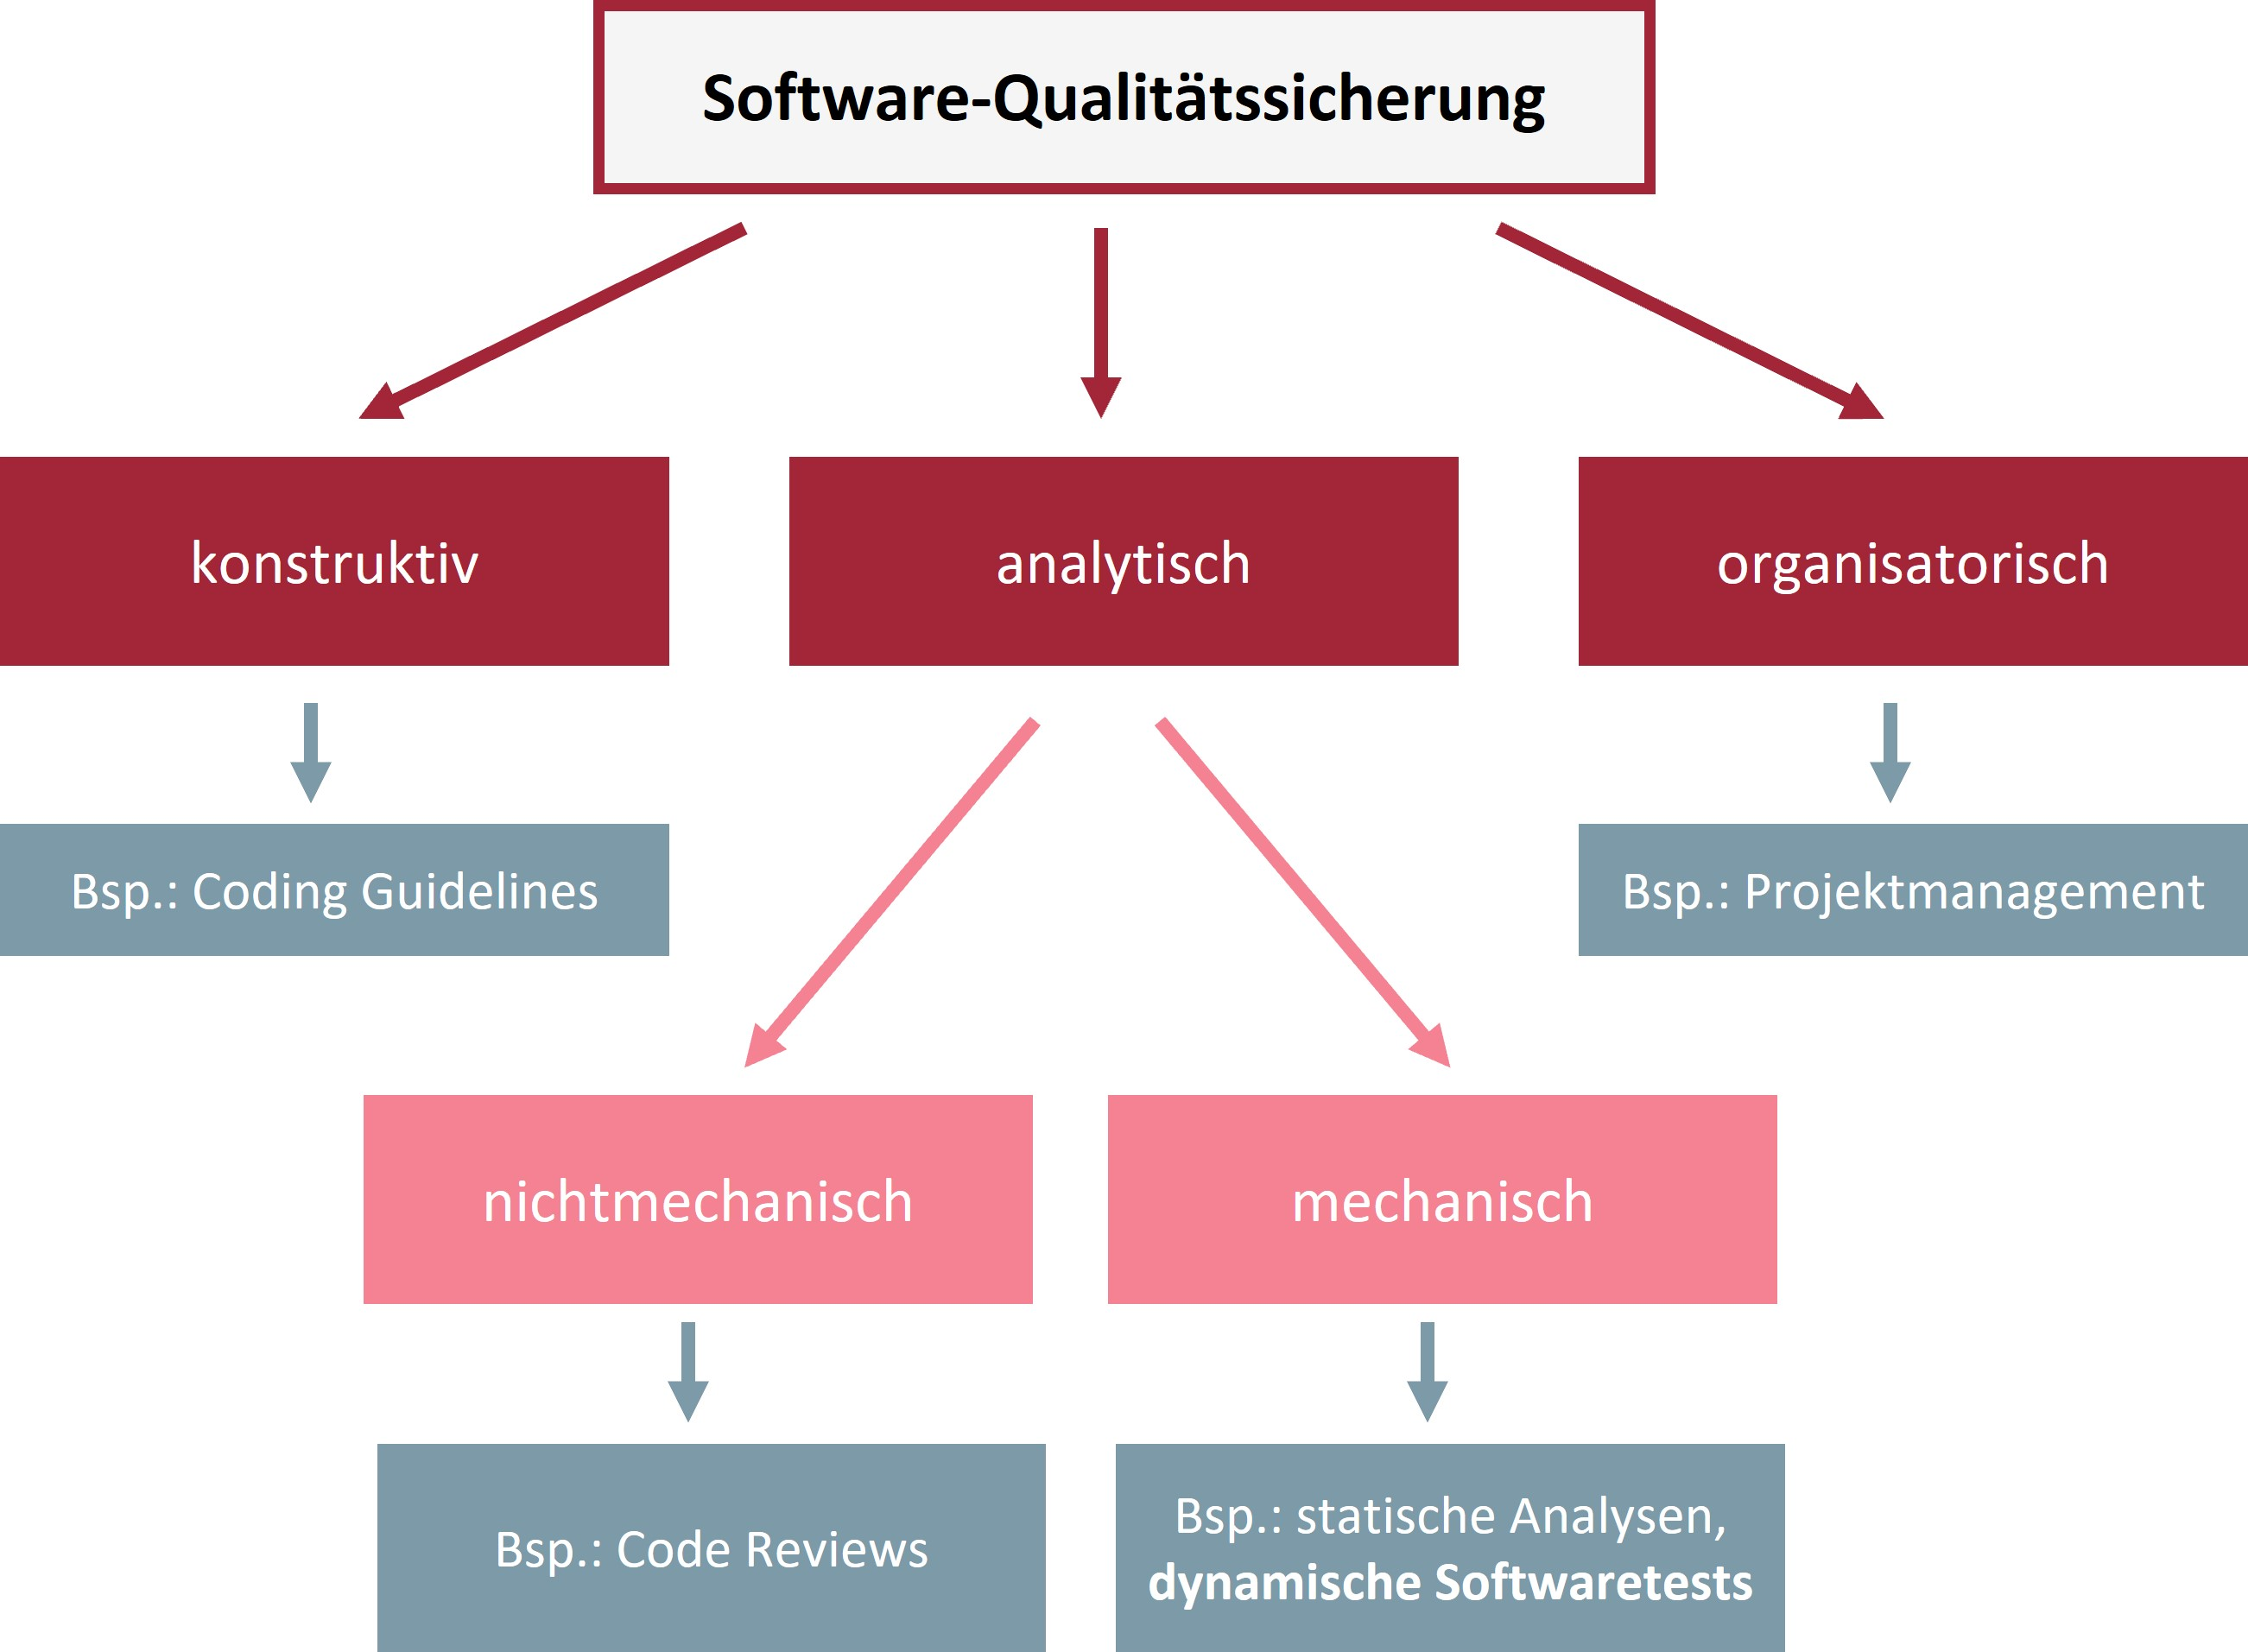
\includegraphics[width=0.5\columnwidth]{images/Qualitaetssicherung_Uebersicht.jpg}
\caption{Die verschiedenen Komponenten der Qualitätssicherung in der Software-Entwicklung in der Übersicht \cite[S. 271]{ludewig2010software}.}
\label{fig:qualitaetssicherung}
\end{figure}


Als Teilgebiet der Qualitätssicherung ist das dynamische Softwaretesten also ein wesentlicher Bestandteil bei der Sicherstellung der Produktqualität, deren wichtigsten Anforderungskriterien der ISO-/IEC-Standard 25010 \cite{ISO25010} als internationale Norm für Software und IT-Systeme zusammenfasst: Im Kern werden dabei von Softwareprojekten eine hohe Funktionalität, Effizienz, Sicherheit, Kompatibilität, Verlässlichkeit, Usability, Wartbarkeit und Portierbarkeit gefordert.

Dynamische Softwaretests besitzen demnach im übergeordneten Sinne die Aufgabe, diese Anforderungen zu prüfen und sicherzustellen. Im Konkreten bedeutet dies, dass dynamische Softwaretests anhand vordefinierter Testfälle mögliche Fehler vor der tatsächlichen Nutzung der Software aufdecken sollen und zudem überprüfen, ob ein Softwaresystem die an das System gestellte Spezifikationen erfüllt \cite[S. 246]{sommerville2012software-engineering}. Testfälle werden typischerweise entweder anhand eines systematischen Vorgehens künstlich erstellt oder ergeben sich aus Erfahrungswerten (vgl. dazu \autoref{subsec:beispieleTests}).  

Der Begriff des Fehlers kann dabei im Rahmen des Testens von Software vielschichtig interpretiert werden und nimmt unterschiedliche Rollen ein: Ein Fehlverhalten (engl.: failure) bezieht sich auf ein unerwartetes Ergebnis eines Programms, ein Codefehler (engl.: defect) beschreibt die zugehörigen fehlerhaften Codezeilen und ein Denkfehler (engl.: error) ist der Auslöser eines Codefehlers. Alle drei Fehlerdefinitionen sind eng miteinander verknüpft: Ein Denkfehler kann bereits in der Konzeption dazu führen, dass trotz einer mutmaßlich korrekten Implementierung Codefehler und somit unterschiedliches Fehlverhalten auftreten kann. Gleichzeitig kann es auch bei der Implementierung durch menschliches Versagen zu Codefehlern kommen, die in der Konzeption korrekt waren und somit keinen Denkfehler darstellen. Abbildung \ref{fig:fehler} zeigt die logische Struktur dieser Begrifflichkeiten auf und greift diese Thematik auf.

\begin{figure}[!h]
\centering
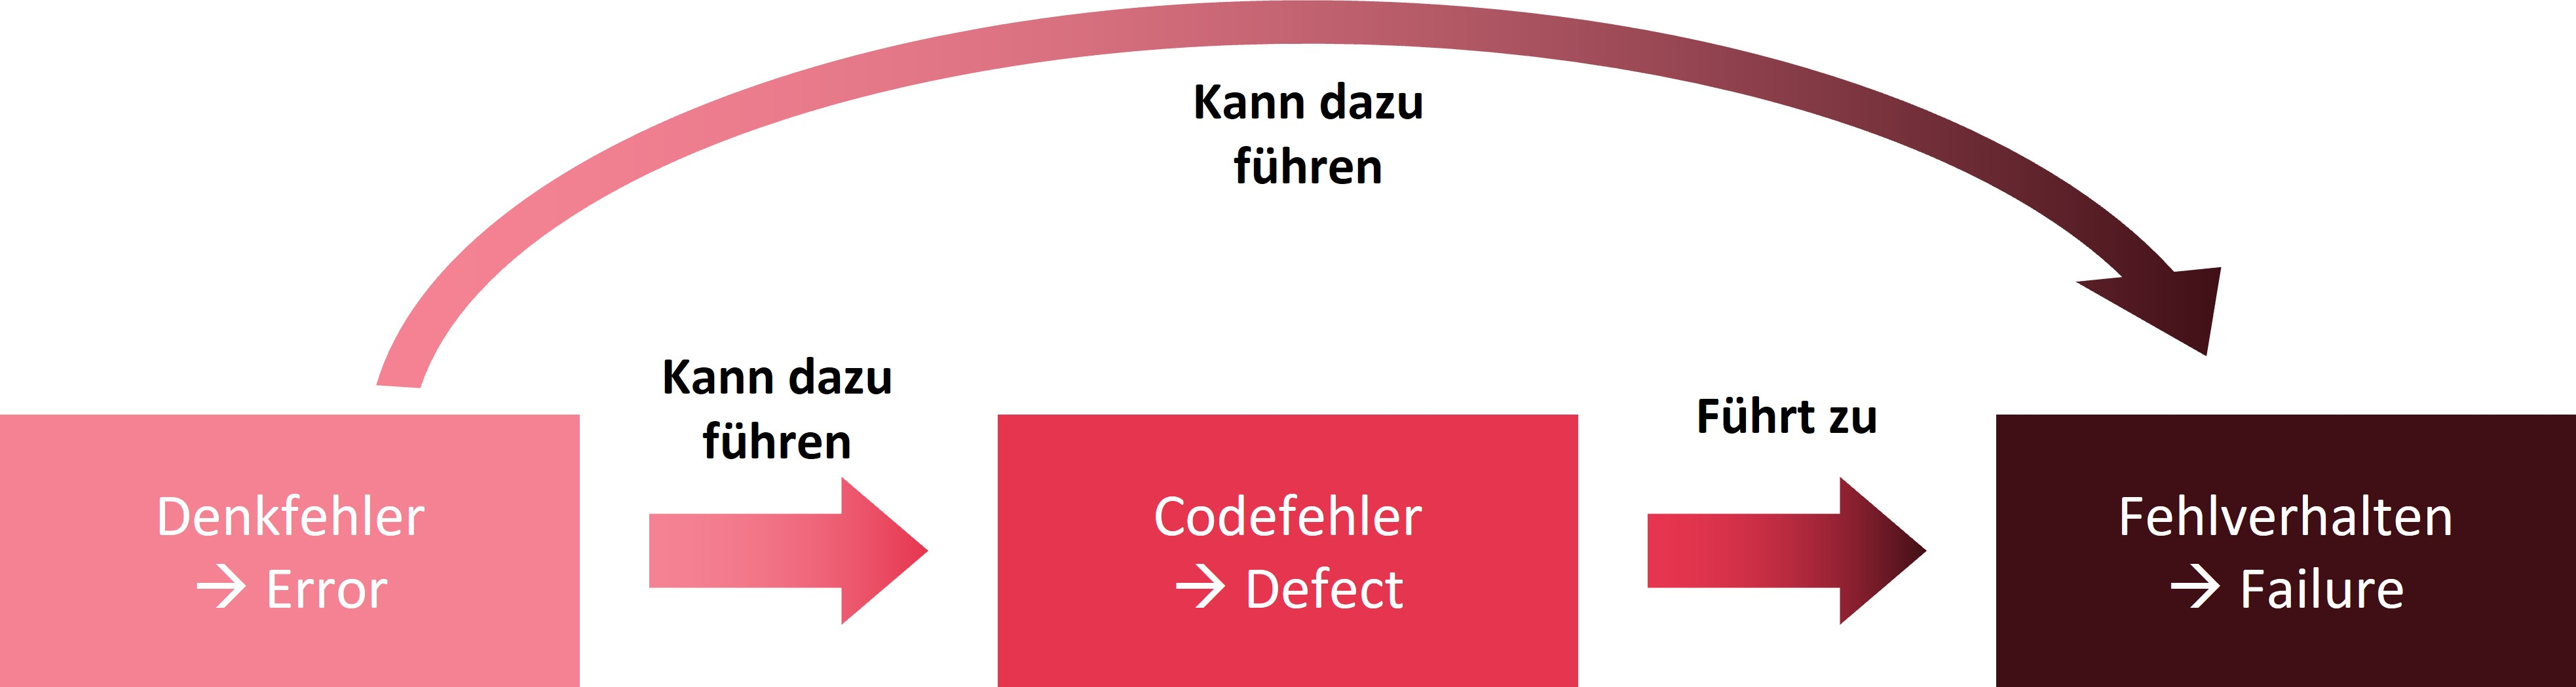
\includegraphics[width=0.8\columnwidth]{images/Fehler_Definition.jpg}
\caption{Ein Denkfehler bei der Implementierung führt zu einem Codefehler, welcher wiederum ein Fehlverhalten der Software auslöst.}
\label{fig:fehler}
\end{figure}

Grundsätzlich gilt es zu berücksichtigen, dass dynamische Softwaretests nicht in der Lage sind, alle Fehler eines Systems vollumfänglich aufzudecken \cite[S. 247]{sommerville2012software-engineering}. Dafür sind die verwendeten Systeme meist zu komplex und vollumfängliche Tests, wie in \autoref{subsec:abdeckung} aufgeführt, nicht umsetzbar. Software-Engineering Pionier Edward Dijkstra stellte in diesem Zusammenhang bereits 1972 fest: 'Tests können nur die Anwesenheit von Fehlern aufzeigen, nicht ihre Abwesenheit' \cite{dahl1972structured}.

Spillner et al. \cite[S. 8]{spillner2011software} fassen die Kernaufgaben, welche dynamische Softwaretests erfüllen sollen, in vier Aspekten zusammen:
\begin{itemize}
\item Entdeckung von Fehlverhalten innerhalb der betroffenen Software
\item Schaffung von Vertrauen in das System bei allen betroffenen Stakeholdern
\item Anregung frühzeitiger Analyse und Dokumentation in der Entwicklung und Wartung um Codefehler zu verhindern
\item Messung von Software-Qualität durch Metriken wie zum Beispiel die Anzahl an Codezeilen, die zyklomatische Komplexität von McCabe \cite{mccabe1976complexity} oder Halsteads-Softwaremetriken \cite{halstead1977elements}
\end{itemize}

\subsection{Testfall-Design}\label{subsec:testfallDesign}

Dynamische Softwaretests werden durch mehrere konkrete Tests an einem bestimmten Testsystem durchgeführt. Jeder Test unterliegt dabei einem spezifischen Testfall, der alle erforderlichen Komponenten zur Durchführung eines Tests bereithält. Diese sind die komplette Systemumgebung, Eingabedaten und das erwartete Verhalten beziehungsweise die erwartete Ausgabe des Systems \cite[S. 86]{schneider2012abenteuer}. 

Ein Testfall sollte dabei auf sinnvolle Art und Weise entwickelt werden: Dazu gehört laut Ludewig und Lichter \cite[S. 480]{ludewig2010software} eine eindeutig definierte Systemumgebung, ein systematisches Vorgehen bei der Wahl der Eingabedaten, klare Kriterien zur Testevaluation und eine detaillierte Dokumentation der Testergebnisse. Wenn diese vier Aspekte auf einen Testfall zutreffen, sprechen Ludewig und Lichter von einem 'systematischen Test'.

Eine der wesentlichen Herausforderungen des dynamischen Softwaretestens besteht darin, ein derartiges systematisches Vorgehen zu entwickeln, um Testfälle möglichst effizient zu erzeugen: Grundsätzlich ist das Ziel des Testfall-Designs mit möglichst wenig Aufwand, also einer geringen Anzahl an Testfällen, möglichst viele Fehler im Sinne eines Fehlverhaltens zu entdecken \cite[S. 498]{ludewig2010software}. Dabei sollte laut Ludewig und Lichter \cite[S. 498]{ludewig2010software} ein Testfall möglichst repräsentativ für viele andere Testfälle sein und zudem idealerweise sehr fehlersensitiv und redundanzarm.

Um diese Anforderungen abdecken zu können wurden in der Vergangenheit verschiedene Techniken ausgearbeitet, die ein systematisches und effizientes Testfall-Design vereinfachen sollen. Dabei entstanden verschiedene Grundprinzipien, die sich aus einer unterschiedlichen Betrachtungsweise auf ein Softwaresystem ergeben. Diese sind nicht komplementär zu verstehen, sondern vielmehr ergänzend zur genauen Spezifizierung der Testfälle. Im Folgenden werden drei relevante Betrachtungsweisen vorgestellt: Stufenbasiertes Testen, Black Box- \& White-Box-Tests und Abdeckungsbasiertes Testen.

Konkrete Testmethoden wie beispielsweise Combinatorial Testing (vgl. \autoref{sec:combinatorialTesting}) oder die Äquivalenzklassenmethode (vgl. \autoref{subsec:beispieleTests}) lassen sich demnach meist unterschiedlichen Bereichen der aufgeführten Betrachtungsweisen zuordnen: So ist die Äquivalenzklassenmethode genauso wie das Combinatorial Testing auf fast allen Stufen des stufenbasierten Testens anwendbar, aber zugleich dem Black-Box-Ansatz zuzuordnen. Im Bereich des abdeckungsbasierten Testens spielt die Äquivalenzklassenmethode zudem bei der Abdeckung der Eingabewerte eine wichtige Rolle.

\subsubsection{Stufenbasiertes Testen}\label{subsec:stufen}

Das stufenbasierte Testen ist eine der abstraktesten Betrachtungsweisen im Hinblick auf die Erstellung von Testfällen: Basierend auf verschiedenen Stufen innerhalb eines Softwareprojekts werden beim stufenbasierten Testen Testfälle passend zu den Anforderungen und Aktivitäten im jeweiligen Stadium des Projekts erarbeitet \cite[S. 5]{ammann2008introduction}. 

Dabei kann auf verschiedene Stufen klassischer Prozessmodelle in der Softwareentwicklung zurückgegriffen werden: Häufig dient dabei das V-Modell als Basis, das im Auftrag des Bundesministeriums für Verteidigung entwickelt wurde und in der Softwarewelt in angepasster Form verbreitete Anerkennung fand \cite[S. 190]{ludewig2010software}. Das V-Modell ist als eine Weiterentwicklung des von Royce \cite{royce1987managing} 1970 entwickelten Wasserfallmodells zu verstehen: Dieses sieht vor, dass die Entwicklung eines Produkts im Allgemeinen in verschiedene Phasen unterteilt werden, bei der jede vorhergehende Phase essenzielle Grundlage der folgenden Phase ist \cite[S. 57 f.]{sommerville2012software-engineering}. Das V-Modell erweitert diesen Ansatz, indem aus jeder dieser Phasen des V-Modells Testfälle passend zu den jeweiligen Aktivitäten dieser Phase abgeleitet werden \cite[S. 190]{ludewig2010software}. %Bei der Anwendung von Test-Driven-Development \cite{beck2003test} werden die Testfälle dabei zusätzlich vor der eigentlichen Formulierung der Spezifikation beziehungsweise Implementierung vorgenommen. 

Üblicherweise werden dabei die folgenden Phasen aus dem Wasserfall- und V-Modell übernommen und daraus resultierende Testfälle unterschieden \cite[S. 5 f.]{ammann2008introduction}. Abbildung \ref{fig:vmodell} visualisiert die hierarchische Struktur und das Zusammenspiel der verschiedenen Stufen des V-Modells:
\begin{itemize}
\item Anforderungsanalyse \& Abnahmetests: Zu Beginn eines jeden Softwareprojekts  werden die konkreten Anforderungen in Zusammenarbeit mit dem Auftraggeber herausgearbeitet. Diese Anforderungen werden in einem abschließenden Stadium eines Projekts anhand von Abnahmetests mittels echter Daten von tatsächlichen oder potenziellen Nutzern getestet.
\item Systemarchitektur \& Systemtest: Beim Systementwurf werden konkrete Designentscheidungen bezüglich der grundlegenden Architektur von Software beschlossen, insbesondere die Zuordnung bestimmter Anforderungen an unterschiedliche Hard- und Softwarekomponenten. Aus dieser Phase resultieren Systemtests, die sämtliche Komponenten des Projekts auf Basis der Architektur testen. 
\item Systementwurf \& Integrationstest: Während der Systementwurf sich auf die grundlegende Architektur fokussiert, werden in der Phase des Subsystementwurfs die konkreten Strukturen und Komponenten der zu entwickelnden Software spezifiziert. Um die Interoperabilität dieser verschiedenen Komponenten zu testen, werden Integrationstests formuliert.
\item Software-Design/Implementierung \& Modul-/Unit-Tests: Die Implementierung umfasst die konkrete Umsetzung des Softwareentwurfs in Programmcode. Jede der einzelnen Komponenten, die meist unabhängig voneinander entwickelt werden, können mittels Unit-Tests bezogen auf kleine Einheiten wie Packages, Methoden oder Klassen getestet werden. Je nach Komplexität des Softwaresystems können weitere übergeordnete Module oberhalb der kleinsten Einheiten ausgearbeitet werden. Bevor letztlich mehrere Komponenten gemeinsam getestet werden, können einzelne Module vorgeschaltet in Modultests geprüft werden.
\end{itemize}

\begin{figure}
\centering
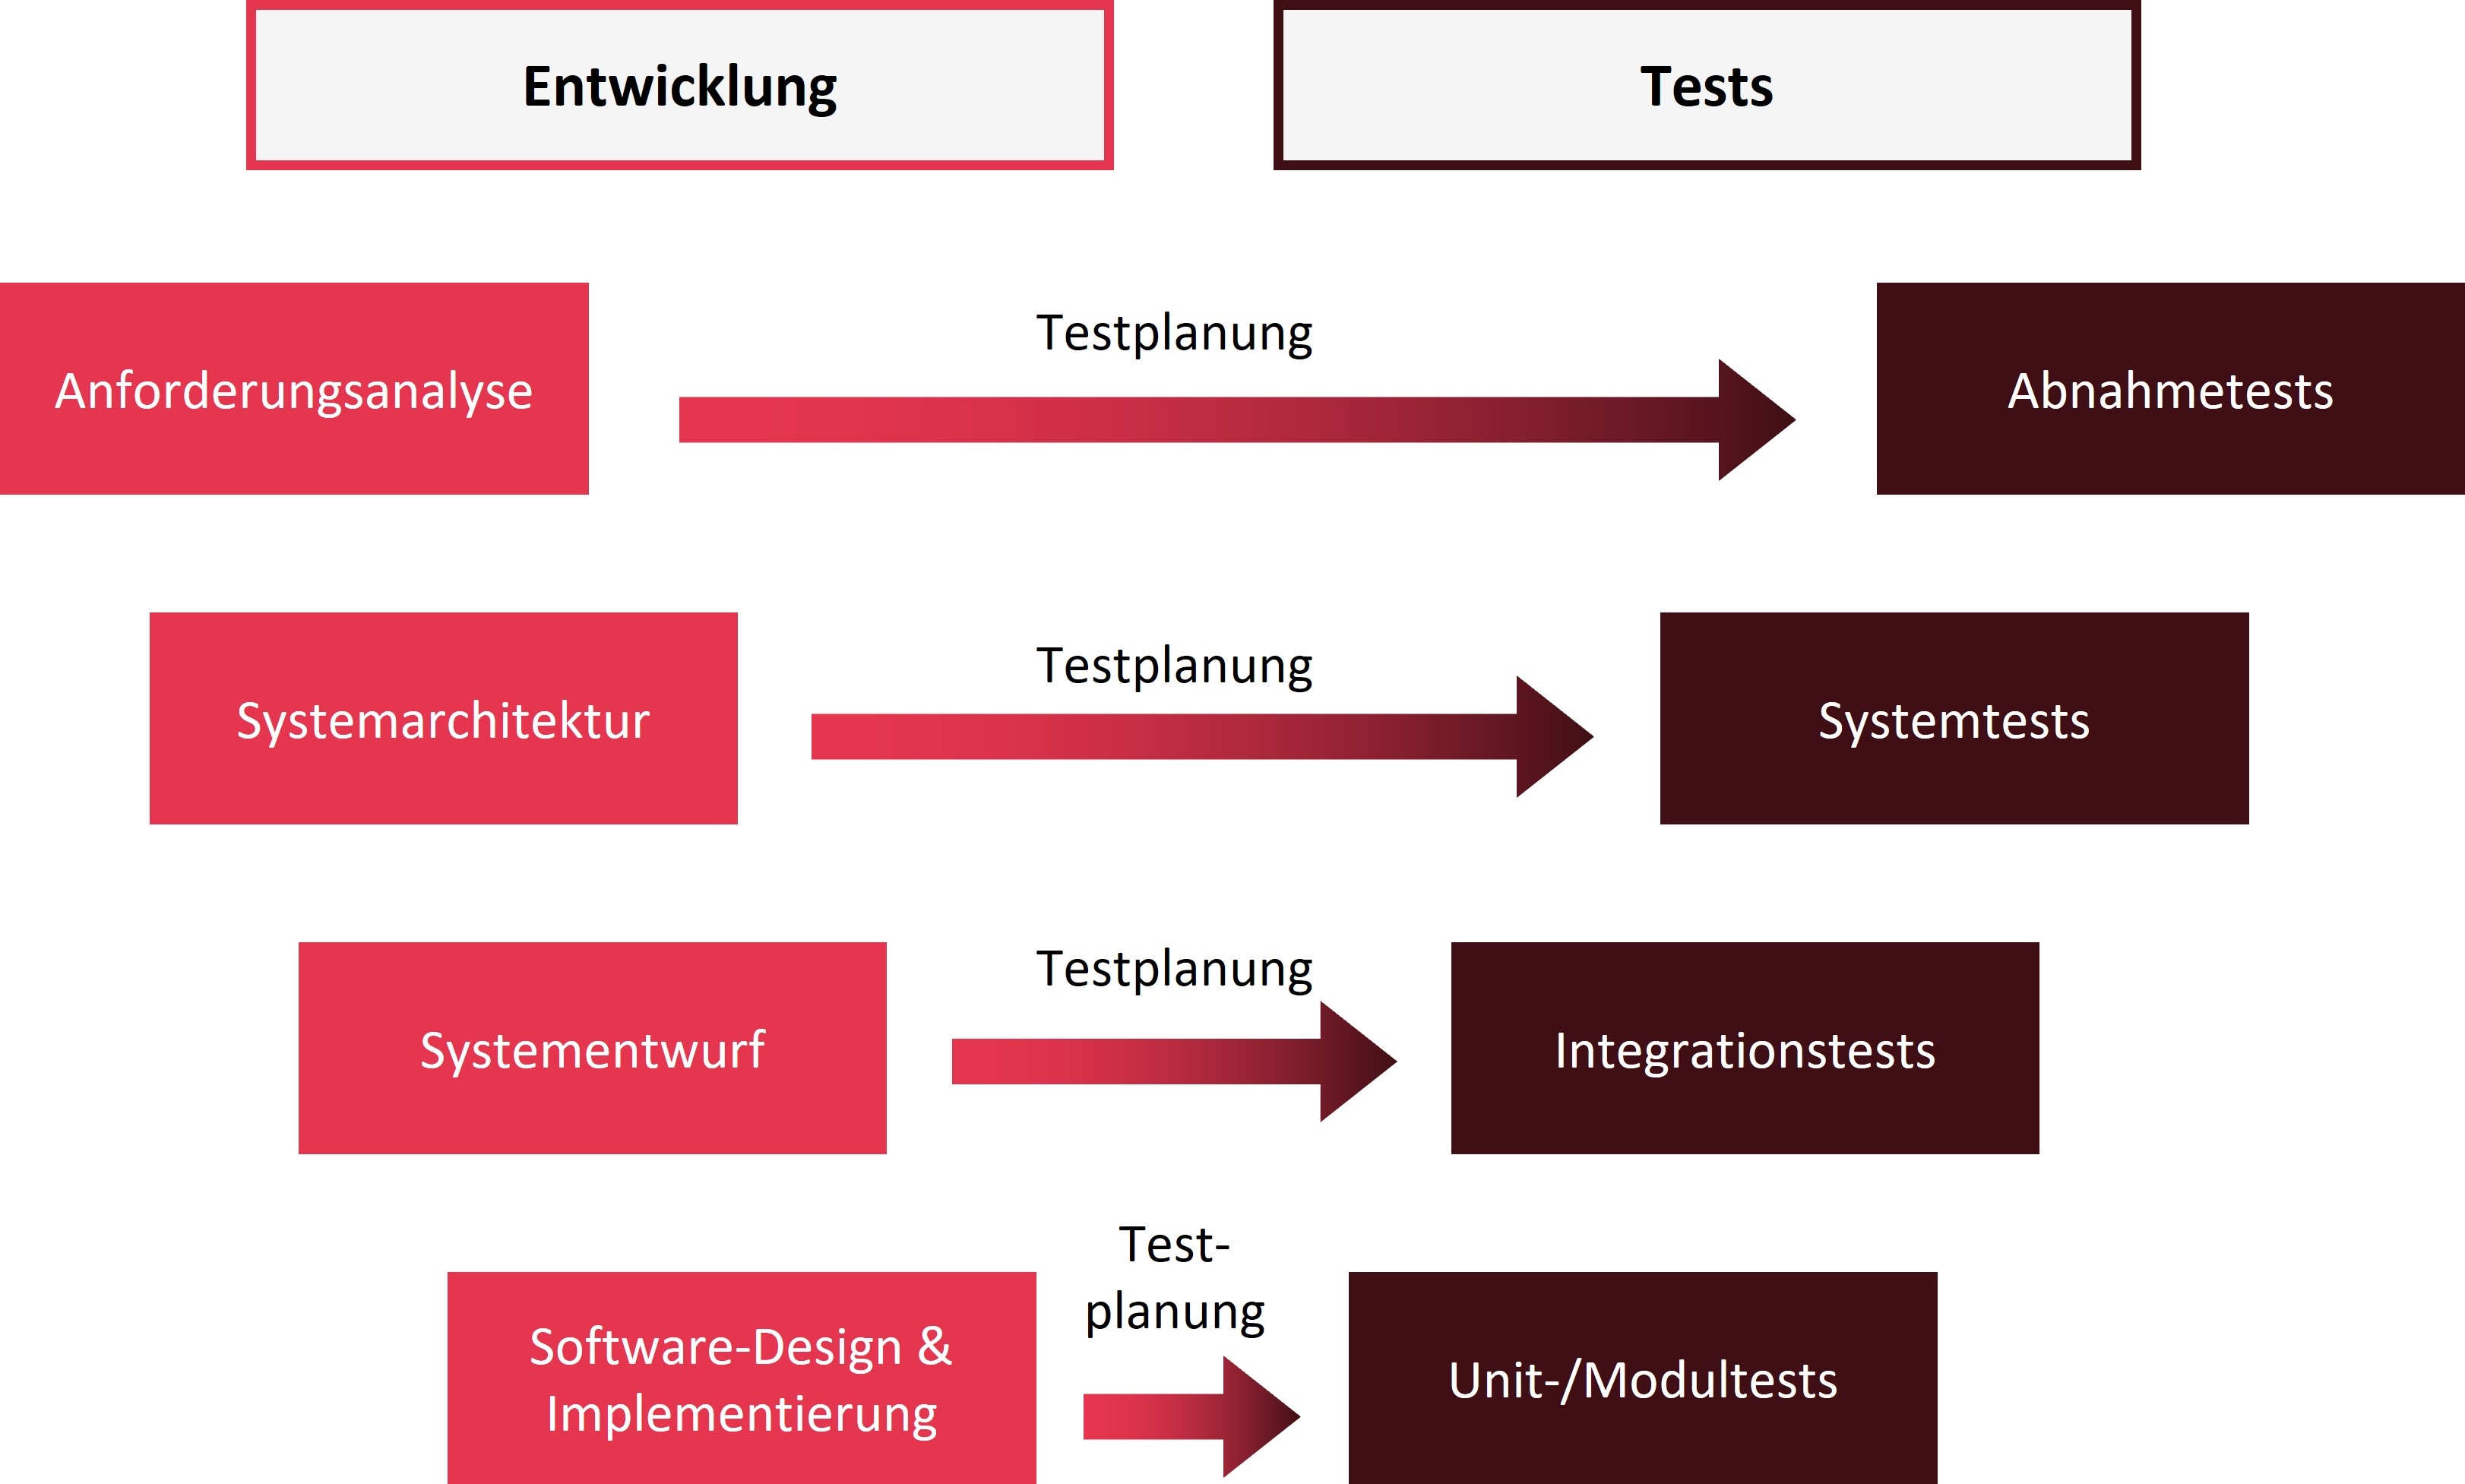
\includegraphics[width=0.7\columnwidth]{images/V_Modell.jpg}
\caption{Das V-Modell dient als Grundlage für das stufenbasierte Testen. Verschiedene Phasen im Entwicklungsprozess einer Software werden mit unmittelbaren Testfällen verknüpft \cite[S. 101]{craig2002systematic}.}
\label{fig:vmodell}
\end{figure}


Die Umsetzung des stufenbasierten Testens muss jedoch nicht unbedingt anhand der vorgegebenen Stufen des V-Modells erfolgen, sondern erlaubt auch selbstdefinierte Phasenmodelle: Craig und Jaskiel \cite[S. 98 f.]{craig2002systematic} führen beispielsweise bestimmte Produktrisiken, personelle oder zeitliche Anforderungen als wesentliche Faktoren bei der Stufenbildung auf.

%Unabhängig von der Wahl der Stufen erfordert das stufenbasierte Testen laut Craig und Jaskiel \cite[S. 98]{craig2002systematic} eine klare Struktur und Definition der Teststufen: Als wesentliche Komponenten müssen demnach die betroffenen Stakeholder und deren Interessen, die Hardware, die Software, die Schnittstellen und die notwendigen Daten im Vorfeld genau bestimmt werden.

\subsubsection{White Box- \& Black Box-Tests}\label{subsec:blackboxWhitebox}

Neben der Fokussierung auf die verschiedenen Phasen im Softwareentwicklungsprozess orientiert sich die Literatur bei der Erstellung von Testfällen in den meisten Fällen an der Unterscheidung zwischen Black-Box- und White-Box-Tests. Dabei bezieht sich der Begriff der White-Box beziehungsweise Black-Box darauf, inwiefern die Struktur der zu testenden Softwareeinheit bei der Erstellung der Testfälle bekannt ist.

\paragraph{Black Box-Tests}

Beim Black-Box-Testen ist die Struktur der zu testenden Softwareeinheit unbekannt, einzig und allein externe Beschreibungen der Software-Spezifikationen dienen als Grundlage für den Testfall \cite[S. 91]{schneider2012abenteuer}. Die Spezifikationen können dabei je nach Entwicklungsstadium im Stufenmodell (vgl. \autoref{subsec:stufen}) unterschiedlich aussehen und somit zu verschiedenen Testfällen führen: So basieren Abnahmetests im Wesentlichen auf dem Black-Box-Ansatz, besitzen aber eine ganz andere Struktur als Unit-Tests, die ebenfalls als Black-Box-Tests durchgeführt werden können.

Grundsätzlich soll laut Schneider \cite[S. 91]{schneider2012abenteuer} im Rahmen von Black-Box-Tests jede Anforderungen an ein System getestet werden. Meist liegen diese nur in Form von Fließtext oder Tabellen vor und müssen dementsprechend in sinnvolle Testfälle umgewandelt werden \cite[S. 92]{schneider2012abenteuer}. Im Falle der Stufe der Anforderungsanalyse und Abnahmetests sind diese schriftlichen Beschreibungen beispielsweise textuelle Erläuterungen der Softwarefunktionalität, bei der Implementierung und Unit-Tests können dies unter anderem Methodenkommentare sein.

Verschiedene Methoden wie beispielsweise die Äquivalenzklassenmethode, die Grenzwertanalyse oder das zustandsbasierte Testen können den Black-Box-Tests zugeordnet werden(vgl. \cite[S. 94 ff.]{schneider2012abenteuer}). Details hierzu folgen in \autoref{subsec:beispieleTests}.

\paragraph{White Box-Tests}

Im Gegensatz zu den Black-Box-Tests setzen White-Box-Tests, oder auch Glass-Box-Tests genannt, voraus, dass die zu testende Softwareeinheit durchsichtig in ihrer Struktur ist und somit Testfälle auf Basis dessen erstellt werden können \cite[S. 91]{schneider2012abenteuer}. Konkret möchte man laut Schneider \cite[S. 91]{schneider2012abenteuer} bei White-Box-Tests kritische Stellen im Programmcode oder an den Schnittstellen verschiedener Softwarekomponenten anhand einer Analyse der vorhandenen Softwarestruktur entdecken.

Die meiste Verwendung finden White-Box-Test auf der Modul- und Implementierungsebene. Dort entsteht laut Schneider durch den hohen Grad an individueller Entwicklungsarbeit oftmals eine hohe Komplexität im Softwaresystem, welche zu schwer ermittelbaren Fehlverhalten im Code führen kann \cite[S. 108]{schneider2012abenteuer}. Daher soll laut Schneider \cite[S. 108 ff.]{schneider2012abenteuer} mit White-Box-Tests im Wesentlichen sichergestellt werden, dass alle geschriebenen Programmteile auch tatsächlich verwendet werden. Dies wird meist mittels Maßen für die Codeüberdeckung umgesetzt: Anweisungsüberdeckung, Zweigüberdeckung und Pfadüberdeckung sind hier die Stichworte, die in der Praxis eine hohe Relevanz besitzen \cite[S. 109 ff.]{schneider2012abenteuer}. 

\subsubsection{Abdeckungsbasiertes Testen}\label{subsec:abdeckung}

Während sich die Literatur in der Vergangenheit bei der Testfallentwicklung im Wesentlichen auf die beiden zuvor aufgeführten Perspektiven der Phasen auf Prozessebene und der Sichtbarkeit der Struktur von Software fokussierte, rückt zunehmend eine weitere dritte Betrachtungsweise in den Fokus der Forschung: Auf Basis von verschiedenen Metriken, welche Abdeckungen bestimmter Eigenschaften des Softwaresystems messen, steht beim abdeckungsbasierten Testen vor allem die Quantifizierung der Güte eines Testverfahrens zur Sicherstellung der Softwarequalität im Fokus \cite{craig2002systematic}. Diese quantitativen Verfahren können unter anderem helfen, verschiedene Stakeholder eines Softwareprojekts von der Güte eines Testbestandes zu überzeugen \cite{kuhn2010practical}.

Neben dem Ansatz, durch verlässliche Metriken Vertrauen in eine Menge von Testfällen zu schaffen, basiert das Konzept des abdeckungsbasierten Testens auf der Erkenntnis, dass ein vollständiges Testen aller denkbaren Zustände, die ein Softwaresystem einnehmen kann, unmöglich ist \cite[S. 16 f.]{craig2002systematic}. Konkret führen Craig und Jaskiel \cite[S. 16]{craig2002systematic} das Beispiel eines Java Compilers an, dessen Limitierung durch die maximale Kapazität des Compiler-Parsers gegeben ist. Der Java Compiler kann theoretisch jede beliebige Zeichenfolge einer .java-Datei aufnehmen, versucht diese anhand seiner internen Logik zu interpretieren und daraus ein ausführbares Programm in Maschinencode zu erzeugen. Die Länge der Eingabe ist durch die Menge an Zeichen limitiert, die der zugehörige Parser aufnehmen kann. Dies entspricht im Falle von Java bei einer maximalen Dateimenge von 64 kB pro Methode \cite{deva_2021} und einer UTF-8-Kodierung mit 1 bis 4 Bytes pro Zeichen mindestens einer Anzahl von 16.000 Zeichen bei voller Auslastung der 64 kB. Berücksichtigt man nun noch alle denkbaren Kombinationen, die durch Permutieren der 144.697 aktuell im Unicode belegten Zeichen \cite{unicode} zustande kommen können, so ergibt sich eine Mindestanzahl von $16.000^{144.697}$ verschiedenen Kombinationen, die ein Java-Parser berücksichtigen müsste: Eine Dimension, die kein Rechner auf dieser Welt testen kann.

Dementsprechend können Testfälle meist nur einen Anteil aller denkbaren Kombinationen abdecken, sodass es sehr hilfreich ist, die Qualität einer Menge an Testfällen beurteilen zu können: Dies wird beim abdeckungsbasierten Testen durch die Nutzung von quantifizierbaren Metriken vorgenommen \cite[S. 17]{craig2002systematic}. Jeder Testfall kann bei seiner Durchführung ein Testkriterium erfüllen oder auch nicht, sodass sich über die gesamte Menge aller zusammenhängender Testfälle ein Anteil ergibt, der die Erfüllung des Testkriteriums im Gesamten quantifiziert \cite[S. 17]{craig2002systematic}. 

Konkret bedeutet dies: Für jedes Abdeckungskriterium lässt sich bestimmen, welche Eigenschaften die Menge aller Testfälle benötigt, um das Kriterium vollständig zu erfüllen. Bei Combinatorial Testing sind dies beispielsweise alle $t$-fachen Kombinationsabdeckungen (vgl. \autoref{subsec:abdeckung}) der Eingabevariablen. Die Quantifizierung der Güte der Menge aller Testfälle ergibt sich schließlich durch die Quote der erfüllten Eigenschaften, die das Abdeckungskriterium fordert. Jeder Testfall kann dann seinen Teil dazu beitragen, dass das betroffene Kriterium erfüllt wird. Dabei kann es passieren, dass mehrere Testfälle den 'gleichen' Beitrag im Sinne des Testkriteriums liefern. In anderen Worten: Manche Testfälle sind überflüssig, da die geforderte Eigenschaft des Abdeckungskriteriums bereits durch einen anderen Testfall oder die Kombination mehrerer Testfälle abgedeckt wird. 

%Grundsätzlich gelten auch beim abdeckungsbasierten Testfalldesign die Prinzipien eines guten Testfalldesigns mit einer hohen Fehlererkennungsrate bei möglichst geringem Testaufwand \cite[S. 20 f.]{craig2002systematic}. Zudem lassen sich manche Abdeckungskriterien insofern vergleichen, als sich diese gegenseitig ergänzen: Beispielsweise ist im Falle der Codeüberdeckung (vgl. \autoref{subsec:beispieleTests}) die Zweigüberdeckung als eine Erweiterung der Anweisungsüberdeckung zu verstehen.

Craig und Jaskiel \cite{craig2002systematic} unterscheiden vier wesentliche Kategorien von Abdeckungen im Bereich des dynamischen Softwaretestens. 
\begin{itemize}
\item Graphen-basierte Abdeckung orientiert sich an verschiedenen Graphstrukturen, die sich im Rahmen eines Softwarekonzepts ergeben wie beispielsweise die Verzweigungen und Wiederholungen innerhalb des Programmcodes. Dabei können Metriken wie Knoten- oder Kantenabdeckungen zur Quantifizierung der Abdeckung herangezogen werden \cite[S. 27 ff.]{craig2002systematic}.
\item Logische Abdeckung basiert auf den Prinzipien der Prädikatenlogik, die sich analog zu Graphstrukturen auf verschiedene Bereiche eines Softwaresystems anwenden lassen, unter anderem die Verzweigungen innerhalb des Programmcodes oder die Umformulierung von Anforderungsspezifikation in Wenn-dann-Verbindungen \cite[S. 131 ff.]{craig2002systematic}. Die Abdeckung der daraus abgeleiteten Testfälle können mit Methoden der Prädikatenlogik wie beispielsweise der Klausel- und Prädikatenabdeckung gemessen werden \cite[S. 106 ff.]{craig2002systematic}.
\item Die Abdeckung der möglichen Eingabewerte berücksichtigt die Grundvoraussetzung jedes Softwaresystems: Jedes Programm verwendet in gewisser Weise Eingaben, sodass alle beliebigen Softwaretests auch Elemente des Eingabeuniversums verwenden \cite[S. 150]{craig2002systematic}. Insbesondere dann, wenn die Struktur einer Software unbekannt ist, stellt die Analyse der möglichen Eingaben und Ausgaben gemeinsam mit der Anwendung von Erfahrungswerten die einzige Möglichkeit zum Testen von Softwareeinheiten dar. Im Vergleich zu den anderen abdeckungsbasierten Ansätzen stehen beim expliziten Testen der Eingabewerte die kombinatorischen Eingabemöglichkeiten im Vordergrund \cite[S. 150 ff.]{craig2002systematic}. Combinatorial Testing ist dabei die relevanteste Methode zur Umsetzung dieser Strategie, welche im Folgenden in \autoref{sec:combinatorialTesting} ausführlich vorgestellt wird. 
\item Syntax-basierte Abdeckung verwendet die Ideen der Automatentheorie und benutzt dabei syntaktische Beschreibungen von zu testenden Softwareeinheiten, um Testfälle abzuleiten \cite[S. 170 ff.]{craig2002systematic}. Im Zusammenhang mit Programmcode spielt vor allem der Begriff der Mutationen eine wichtige Rolle, bei dem elementare Codestücke durch leichte Veränderungen ersetzt werden und so Fehlverhalten provoziert wird. Als Metrik werden dabei zumeist die Abdeckung der Symbole und Produktionsregeln und weitere komplexere Kombinationen verwendet \cite[S. 172]{craig2002systematic}.
\end{itemize}

\begin{comment}
Craig und Jaskiel \cite{craig2002systematic} unterscheiden vier wesentliche Kategorien von Abdeckungen im Bereich des Softwaretestens. 
\begin{itemize}
\item Graphen-basierte Abdeckung: Typischerweise verbindet man Graphen in den ersten Phasen des Softwareentwicklungsprozesses der Anforderungsanalyse und der Systemarchitektur mit Anwendungsfalldiagrammen oder Aktivitätsdiagrammen. Weitere Graphstrukturen lassen sich zudem auf der Modul- und Implementierungsebene bei Komponenten- und Klassendiagrammen finden. Im Zusammenhang mit der Generierung von Testfällen sind jedoch vor allem Zustandsmaschinen und insbesondere Anweisungsabläufe und Datenflüsse weit verbreitet. All diese Graphenmodelle können laut Craig und Jaskiel \cite[S. 27 ff.]{craig2002systematic} auf Basis verschiedener Graphen-basierter Metriken getestet werden. Dabei unterscheiden die beiden Autoren zwischen Abdeckungskriterien der strukturellen Eigenschaften und des Datenflusses der zu testenden Softwareeinheit. Beide Varianten fokussieren sich auf verschiedene Metriken der Knoten- und Kantenabdeckung beziehungsweise komplexeren Messzahlen der erzeugten Graphstruktur \cite[S. 33 ff.]{craig2002systematic}.
\item Logische Abdeckung: In recht ähnlicher Art und Weise wie bei der Graphen-basierten Abdeckung orientieren sich die Testprinzipien der logischen Abdeckung in den meisten Anwendungsfällen an den Verzweigungen innerhalb des Programmcodes. Wenn-dann-Beziehungen und Wiederholungen können dabei in prädikatenlogische Aussagen umgewandelt werden, die schließlich als Grundlage für die Erzeugung von Testfällen dienen \cite[S. 120 ff.]{craig2002systematic}. Neben diesem strukturbasierten Ansatz (analog zu einer White-Box-Strategie) lässt sich das Prinzip der Prädikatenlogik auf die Ebene der Spezifikation von verschiedenen zu testenden Softwareeinheiten übertragen, indem Vorbedingungen an den Testprüfling in prädikatenlogische Aussagen formuliert werden \cite[S. 131 ff.]{craig2002systematic}. Zudem führen Craig und Jaskiel die Möglichkeit auf, die Abläufe einer Zustandsmaschine in prädikatenlogische Aussagen umzuformulieren und diese zu testen \cite[S. 134 ff.]{craig2002systematic}. Als Metrik werden bei der logischen Abdeckung in verschiedenen Ausprägungen die logisch denkbaren Möglichkeiten mit den tatsächlich getesteten Möglichkeiten abgeglichen (Klausel- und Prädikatenabdeckung) \cite[S. 106 ff.]{craig2002systematic}.
\item Abdeckung der möglichen Eingabewerte: Eingaben und Ausgaben sind wesentliche Grundprinzipen einer jeden Software, sodass jede Art eines Softwaretests in gewisser Form Elemente des Eingabeuniversums verwendet \cite[S. 150]{craig2002systematic}. Bei den zuvor aufgeführten Varianten der Graphen-basierten und logischen Abdeckung steht jedoch das Universum aller möglichen Eingaben selbst nicht im Mittelpunkt, sondern vielmehr die Struktur und die Zusammenhänge innerhalb der Software. Beim Testen der Eingabewerten ist dies der Fall: Im Konkreten werden dabei die Eingabedomäne einer Softwareeinheit in verschiedene Mengen unterteilt und anschließend anhand kombinatorischer Metriken die Qualität der resultierenden Softwaretests ermittelt \cite[S. 150 ff.]{craig2002systematic}. Dabei kann laut Craig und Jaskiel im Wesentlichen zwischen einer unabhängigen Betrachtungsweise auf einzelne Parameter, also beispielsweise die verschiedenen denkbaren Werte einer Variablen, und einer gesamtheitlichen Sichtweise auf die Funktionalität im Zusammenspiel verschiedener Parameter unterschieden werden \cite[S. 153 ff.]{craig2002systematic}. Combinatorial Testing (vgl. \autoref{sec:combinatorialTesting}) ist dabei eine der relevantesten Methoden zur Umsetzung dieser Strategie.
\item Syntax-basierte Abdeckung: Die Grundidee des Syntax-basierte Testens stammt im Wesentlichen aus Bereichen der Automatentheorie und verwendet syntaktische Beschreibungen von zu testenden Softwareeinheiten um Testfälle abzuleiten \cite[S. 170 ff.]{craig2002systematic}. So lässt sich beispielsweise ein Programmiersprache über eine BNF-Grammatik mit verschiedenen Symbolen und Produktionsregeln definieren, die als Grundlage für eventuelle Testfälle dienen. Als Metrik werden dabei die Abdeckung der Symbole und Produktionsregeln und weitere komplexere Kombinationen verwendet \cite[S. 172]{craig2002systematic}. Im Zusammenhang mit Programmcode spielt jedoch vor allem der Begriff der Mutationen eine wichtige Rolle, bei dem elementare Codestücke durch leichte Veränderungen ersetzt werden. Als Beispiele führen Craig und Jaskiel unter anderem das Austauschen von arithmetischen Operationen an \cite[S. 182 ff.]{craig2002systematic}. Die Mutationen sollten in den meisten Fällen zu einem unerwünschten Verhalten der Software führen, sodass beispielsweise gemessen werden kann, wie häufig diese zu Fehlern führen \cite[S. 178 f.]{craig2002systematic}.
\end{itemize}
\end{comment}


\subsection{Beispiele für Teststrategien}\label{subsec:beispieleTests}

Der folgende Abschnitt greift die grundlegende Herangehensweise in Bezug auf das dynamische Softwaretesten aus \autoref{subsec:testfallDesign} auf und führt einige konkrete Beispiele für Teststrategien ein. Diese Beispiele beschränken sich auf mögliche Anwendungen im Zusammenhang mit dem in \autoref{chap:anwendungsfall} vorgestellten Anwendungsfall. Da dieser sich im Wesentlichen auf einen spezifikationsbezogenen Ansatz fokussiert, werden insbesondere die Techniken des White-Box-Testens (vgl. \autoref{subsec:blackboxWhitebox}) an dieser Stelle ausgeklammert. Detaillierte Ausführungen zu den verbreiteten White-Box-Strategien der Anweisungs-, Zweig- und Pfadüberdeckung lassen sich in \cite[S. 108 ff.]{schneider2012abenteuer} nachlesen.

Da der Fokus dieser Arbeit auf Combinatorial Testing liegt, werden zudem die Prinzipien dieser Teststrategie nicht an dieser Stelle, sondern im folgenden, separaten \autoref{sec:combinatorialTesting} vorgestellt.

\subsubsection{Äquivalenzklassenmethode}

Da vollständiges Testen - wie zuvor erläutert - nicht möglich ist, erfordern systematische Tests Einschränkungen bei der Wahl der Parameter. Die Äquivalenklassenmethode löst dieses Problem derart, dass alle denkbaren Eingaben in verschiedene Äquivalenzklassen partitioniert werden \cite[S. 94]{schneider2012abenteuer}. Dabei sollten laut Schneider \cite[S. 94 ff.]{schneider2012abenteuer} die unterschiedlichen Klassen derart konstruiert werden, dass Vertreter aus derselben Klasse sich in Bezug auf das Fehlerverhalten innerhalb der Software identisch verhalten. Als Beispiel führt Schneider eine automatisierte Schwimmbadkasse auf, die für Jugendliche unter 18 Jahre einen vergünstigten Preis anbietet. In diesem Fall würde sich eine Äquivalenzklasse für die Variable 'Alter' durch die Menge 'Jugendlich' $= \{n < 18 ~ | ~ n \in \N\}$ und eine weitere Klasse 'Erwachsen' $= \{n \geq 18 ~ | ~ n \in \N\}$ ergeben. 

Je nach Spezifikation und denkbaren Eingaben müssen die Äquivalenzklassen auch mögliche Falscheingaben berücksichtigen. Eine wesentliche Herausforderung bei Anwendung der Äquivalenzklassenmethode besteht laut Schneider darin, eine passende Auswahl der Klassen zu treffen, die einerseits nicht zu kleinteilig, andererseits aber auch nicht zu pauschalisierend sein sollte \cite[S. 95]{schneider2012abenteuer}.

\subsubsection{Grenzwertanalyse}

Die Grenzwertanalyse basiert auf der Annahme, dass es häufig unmittelbar an den Grenzen verschiedener Eingabeparameter zu Fehlverhalten kommt, da diese oftmals nicht genau definiert sind oder von Programmierenden nicht berücksichtigt werden \cite[S. 120]{spillner2011software}. Dementsprechend überprüft die Grenzwertanalyse die Grenzen kritischer Werte und stellt somit eine Erweiterung der Äquivalenzklassenmethode dar \cite[S. 120 f.]{spillner2011software}. 

Für jede Äquivalenzklasse ergeben sich laut Spillner et al. \cite[S. 120 f.]{spillner2011software} automatisch kritische Grenzen, die mittels der Grenzwertanalyse abgedeckt werden können. Im Beispiel der Schwimmbadkasse würde dies bedeuteten, dass ein besonderes Augenmerk auf die Werte 17 und 18 gelegt werden sollte. Neben diesen offensichtlichen Grenzen der verschiedenen Äquivalenzklassen werden im Rahmen der Grenzwertanalyse häufig auch extreme, unerwartete Werte wie beispielsweise die maximal oder minimal mögliche Eingabe berücksichtigt werden \cite[S. 122]{spillner2011software}. Sowohl die Grenzwertanalyse als auch die Äquivalenzklassenmethode lässt sich auf allen Ebenen des Stufenmodells (vgl. \autoref{subsec:stufen}) anwenden und ist in Bezug auf das abdeckungsbasierte Testen vor allem im Bereich der Abdeckung der Eingaben relevant.

\subsubsection{Zustandsbasiertes Testen}

Zustandsbasiertes Testen basiert auf der grundlegenden Annahme, dass sich jeder deterministische Programmfluss einer Software durch einen endlichen Automaten mit verschiedenen Zuständen und exakt definierten Zustandsübergängen darstellen lässt. Die Darstellung eines endlichen Automaten kann über ein Graph-basiertes Modell (vgl. \autoref{subsec:abdeckung}) oder über eine Zustandsübergangstabelle erfolgen. Als Teststrategie eines Zustandsautomaten ergibt sich die Methode, dass jede einzelne Zelle der Zustandsübergangstabelle einen Testfall ergibt. Dadurch, dass die Transition der betroffenen Zustände im endlichen Automat eindeutig definiert sind, fällt die Ableitung der notwendigen Werte betroffener Parameter leicht. 

Das zustandsbasierte Testen spielt insbesondere dann eine wichtige Rolle, wenn Systeme verschachtelte Hierarchien besitzen. Im Anwendungsfall dieser Arbeit (vgl. \autoref{chap:anwendungsfall}) wird dies insbesondere bei Eingabemasken relevant, die nur durch die bestimmte Auswahl eines spezifischen Parameters zum Einsatz kommen und in allen anderen Fällen nicht. 

\subsubsection{(Adaptive) Random Testing}

In einigen Fällen möchte man eine Softwareeinheit testen, bei der weder eine detaillierte Beschreibung der Spezifikation, noch der Programmcode selbst vorliegt. Dafür bietet sich die Verwendung des Zufallsprinzips an, welche die Grundlage des Random Testings ist. Dabei wird für das Eingabeuniversum eine Wahrscheinlichkeitsverteilung angenommen, aus welcher Eingabewerte zufällig entnommen werden \cite[S. 141 f.]{spillner2011software}. Grundsätzliche Vorteile einer zufallsbasierten Teststrategie ergeben sich laut Spillner \cite[S. 142]{spillner2011software} vor allem durch eine realitätsnahe Abbildung der tatsächlich verwendeten Werte der Softwareeinheit und durch die Möglichkeit, statistische Methoden zur Quantifizierung der Systemzuverlässigkeit anwenden zu können.

Unter anderem White und Cohen \cite{white1980domain} konnten herausfinden, dass Fehlverhalten meist sehr gebündelt in Bereichen von Eingabewerten auftreten, sodass bereits durchgeführte Testfälle, die kein Fehlverhalten aufdeckten, möglichst weit im Eingabeuniversum von neuen Testfällen entfernt sein sollten \cite{survey2013}. Aus diesem Grund entwickelten Chen et al. \cite{chen2004adaptive} die Methode des Adaptive Random Testing, welche versucht, die Testfälle möglichst weit und gleichmäßig über das Eingabeuniversum zu verteilen. Verschiedene Strategien und Algorithmen auf Basis von Distanzmaßen, Ausschlussverfahren oder evolutionären Algorithmen wurden in der Vergangenheit entwickelt, um Adaptive Random Testing in der Praxis umzusetzen \cite{huang2012adaptive}.

\subsubsection{Erfahrungsbasiertes Testen}

Neben den aufgeführten systematischen Ansätzen Testfälle zu Erzeugung existiert eine weitere Methode zur Testfallerzeugung, die in der Anwendungspraxis eine bedeutende Rolle spielt: Erfahrungsbasiertes Testen kann vor allem Fehler aufdecken, die systematische Ansätze übersehen \cite[S. 210]{spillner2010basiswissen}. Das Wissen und die Expertise der testenden Person bildet dabei die Grundlage, um mögliche Probleme innerhalb einer Softwareeinheit mit Tests aufzudecken. Spillner et al. \cite[S. 213]{spillner2010basiswissen} betonen, dass erfahrungsbasiertes Testen nicht als erstes Mittel der Wahl bei der Erstellung von Testfällen verwendet werden sollte, sondern vielmehr als Ergänzung anderer systematischer Ansätze zu verstehen ist. 

Insbesondere interagiert das erfahrungsbasierte Testen häufig mit anderen konkreten Testmethoden wie beispielsweise der Äquivalenzklassenmethode oder der Grenzwertanalyse: So stellt die Wahl der Äquivalenzklassen beziehungsweise die Wahl kritischer Grenzwerte eine wesentliche Herausforderung der beiden Testmethoden dar, sodass an dieser Stelle Erfahrungswerte und Expertise besonders hilfreich sein können.

Erfahrungsbasiertes Testen lässt sich nur teilweise den drei zuvor aufgeführten Grundprinzipien des Testens zuordnen und kann selbst nur als 'semi-systematisches' Verfahren bezeichnet werden: Die Methode lässt sich nicht eindeutig als Black Box- oder White Box-Technik einstufen \cite[S. 213]{spillner2010basiswissen}, auch ein Abdeckungskriterium existiert, welches die Güte von erfahrungsbasierten Tests messen kann, existiert in den meisten Fällen nicht. Die Expertise erfahrenerer Tester*innen kann auf allen Ebenen des stufenbasierten Testens nützlich sein, kommt aber meist auf höheren Teststufen zum Einsatz, da auf den niedrigeren Ebenen genügend Informationen über die Spezifikationen, wie beispielsweise der Programmcode selbst, zur Verfügung stehen \cite[S. 213]{spillner2010basiswissen}.

In der Praxis haben sich in Bezug auf erfahrungsbasiertes Testen verschiedene Teilaspekte herausgebildet \cite[S.210 ff.]{spillner2010basiswissen}:
\begin{itemize}
\item 'Error Guessing' (deutsch: Fehlerraten) basiert auf der Idee, Fehler aus der Vergangenheit oder in Zukunft zu erwartende Fehler bei der Testfallerstellung zu berücksichtigen \cite[S.210 f.]{spillner2010basiswissen}.
\item Checklistenbasiertes Testen verwendet eine Checkliste zur Testfallerzeugung, die eine erfahrene Testperson in der Vergangenheit angelegt hat und die als Anleitung für zukünftige Testfälle dient \cite[S. 211 f.]{spillner2010basiswissen}. In diesem Fall kann ein Abdeckungskriterium für die Güte einer Menge von Testfällen definiert werden, indem der Anteil der erfüllten Aspekte der Checkliste ermittelt wird \cite[S. 211]{spillner2010basiswissen}.
\item Exploratives Testen ist ein Verfahren, das einen kontinuierlichen Prozess bestehend aus Testfallerzeugung und Auswertung jener Testfälle beschreibt \cite[S. 211]{spillner2010basiswissen}. Über die Zeit hinweg entwickelt laut Spillner und Linz \cite[S. 212]{spillner2010basiswissen} die testende Person zunehmend mehr Wissen und Verständnis über das Testobjekt und kann dieses für neue, verbesserte Testfälle anwenden. Darüber hinaus kann das Wissen des explorativen Testens angewendet werden, um systematische Tests zu entwickeln.
\end{itemize}

\section{Combinatorial Testing}\label{sec:combinatorialTesting}

Combinatorial Testing (deutsch: Kombinatorisches Testen) ist analog zu den Beispielen aus \autoref{subsec:beispieleTests} eine Strategie zur systematischen Erzeugung von Testfällen. Da diese Methode in dieser Arbeit im Mittelpunkt steht, wird diese nun an dieser Stelle ausführlicher als die zuvor aufgeführten Teststrategien vorgestellt. Zunächst sollen dabei die grundlegende Motivation für Combinatorial Testing und die wesentlichen Prinzipien im Fokus stehen. Anschließend werden verschiedene Metriken zur Quantifizierung der Güte eines Testbestandes im Zusammenhang von Combinatorial Testing erläutert und verschiedene Algorithmen und Tools zur Anwendung von Combinatorial Testing vorgestellt.

\subsection{Einführung in Combinatorial Testing}\label{subsec:einführungCombinatorial}

Als wesentliche Motivation für die Verwendung kombinatorischer Methoden bei der Erzeugung von Testfällen ergibt sich wie bei fast allen Testfallstrategien auch die Erkenntnis, dass vollständige Tests in der Realität nicht umsetzbar sind (vgl. \autoref{sec:einführungTest}). Combinatorial Testing greift diese Tatsache auf und versucht auf effiziente Art und Weise das Eingabeuniversum einer zu testenden Softwareeinheit möglichst sinnvoll mittels kombinatorischer Methoden im Sinne von quantifizierbaren Metriken (vgl. \autoref{subsec:abdeckung}) abzudecken. Dabei kann Combinatorial Testing auf allen Ebenen des in \autoref{subsec:stufen} aufgeführten Stufenmodells zum Einsatz kommen, wie verschiedene Beispiele in diesem Abschnitt aufzeigen werden. Zudem lässt sich Combinatorial Testing als Black-Box-Technik einstufen, da die Struktur der zu testenden Softwareeinheit für den Testablauf irrelevant ist.

Grundannahme beim Combinatorial Testing ist es, dass selten die Eingaben einzelner Parameter eines Testprüflings für Fehler verantwortlich sind, sondern vielmehr die Interaktion einiger weniger Parameter zu häufigen Fehlern führt \cite{kuhn2010practical}. Kuhn et al. \cite{kuhn2004error} konnten in einer Analyse verschiedener Software-Systeme aufzeigen, dass die Interaktion von sechs oder weniger Parameter für annähernd 100 Prozent der auffindbaren Softwarefehler verantwortlich sind. Abbildung \ref{fig:pairwise} zeigt ein einfaches Beispiel aus \cite{kuhn2010practical}, bei welchem nur die Kombination aus den Parametern 'Druck' $< 10$ und 'Volumen' $> 300$ zu einem Fehlverhalten führt. Bei einer zufälligen Wahl der Testparameter könnte es dazu kommen, dass dieses Fehlverhalten nicht aufgedeckt wird.

\begin{figure}[]
\lstset{language=Java}
\begin{lstlisting}[frame=single]
				if ('Druck' < 10) {
					// do something
					if ('Volumen' > 300) {
						// faulty code! BOOM!
					} else {
						// good code, no problem
					}
				} else {
					// do something else
				}
\end{lstlisting}
\caption{Beispiel für die Interaktionsproblematik beim Testen verschiedener Parameter: Nur bei der Kombination 'Druck' $< 10$ und 'Volumen' $> 300$ kommt es zu einem Fehlverhalten \cite{kuhn2010practical}.}
\label{fig:pairwise}
\end{figure}

Um diesem Problem zu begegnen, hat sich laut Kuhn et al. \cite{kuhn2010practical} in der Anwendungspraxis das sogenannte Pairwise-Testing etabliert, bei dem alle Kombinationen von Paaren der Eingabeparameter getestet werden. Im Beispiel von Abbildung \ref{fig:pairwise} bedeutet dies, dass alle vier paarweise Kombinationen aus 'Druck' $< 10$, 'Druck' $\geq 10$, 'Volumen' $> 300$, 'Volumen' $\leq 300$ getestet werden sollten. Der Ansatz des Combinatorial Testing greift diese Idee auf und erweitert die Idee des Pairwise-Testing derart, dass die Zahl des zu prüfenden Interaktionsparameters variabel ist \cite{kuhn2010practical}. Konkret entspricht ein Combinatorial Testing-Ansatz mit Interaktionsparameter $t=2$ dem Pairwise-Konzept, bei $t=3$ muss jede denkbare Dreierkonstellation der Eingabeparameter mindestens in einem Testfall berücksichtigt werden. 

Aus mathematischer Sicht lassen sich daraus eine Mindest- und Maximalanzahl durchzuführender Tests ($T_{\min}$, $T_{\max}$) anhand der Wahl des Interaktionsparameter $t$, der Anzahl $n$ aller Eingabeparameter $x_i$ und der Anzahl $y_i$ der verschiedenen Werte, die jeder Parameter $x_i$ annehmen kann, ermitteln: Unter der Annahme, dass der Interaktionsparameter $t$ größer als die Anzahl $n$ der vorhandenen Parameter ist, stellt das Produkt der $t$ größten Werte $y_i$ eine untere Schranke für die durchzuführenden Tests dar. Seien also die $y_i$ derart geordnet, dass $y_1 \geq y_2 \geq \dots \geq y_n$. Dann gilt:
\begin{gather}
T_{\min} = \prod_{i = 1}^{t} y_i
\end{gather}
Eine obere Schranke für die Anzahl der Tests ist unterdessen die Anzahl aller denkbaren Kombinationen der Eingabeparameter:
\begin{gather}
T_{\max} = \prod_{i=1}^{n} y_i
\end{gather}

Eine große Spannweite zwischen $T_{\min}$ und $T_{\max}$ entsteht insbesondere dann, wenn die Differenz zwischen der Anzahl der Parameter $n$ und des Interaktionsparameters $t$ groß wird. Im Gegensatz dazu liegen $T_{\min}$ und $T_{\max}$ nah beisammen, wenn $n$ und $t$ beinahe identisch sind. Combinatorial Testing kann seine Vorteile vor allem dann ausspielen, wenn die Differenz zwischen $T_{\min}$ und $T_{\max}$ sehr groß ist: Durch die Fokussierung auf die Interaktion von $t$ Parametern können in einem Testfall mehrere Parameterkombinationen gleichzeitig abgedeckt werden, was die Anzahl der tatsächlich benötigten Tests in Relation zu $T_{\max}$ sehr nahe an der unteren Schranke $T_{\min}$ hält.

Das in Tabelle \ref{tab:3wayInteraction} aufgeführte Beispiel aus \cite{kuhn2010practical} verdeutlicht dieses Prinzip: Die Tabelle zeigt eine mögliche Reihe an Testfällen für $n=10$ binäre ($y_i = 2 ~ \forall i = 1,\dots,n)$ Eingabevariablen A bis J bei einer Abdeckung aller Dreierkombinationen, also $t = 3$. Eine derartige Tabelle mit einer vollständigen Abdeckung aller $t$-fachen Kombinationen der Eingabeparameter nennt man im Kontext des Combinatorial Testing auch Covering Array oder Orthogonal Array. 

\begin{table}[h]
\begin{tabular}{|l|l|l|l|l|l|l|l|l|l|}
\hline
\cellcolor{grauinfo}A&\cellcolor{grauinfo}B&\cellcolor{grauinfo}C&\cellcolor{grauinfo}D&\cellcolor{grauinfo}E &\cellcolor{grauinfo}F&\cellcolor{grauinfo}G&\cellcolor{grauinfo}H&\cellcolor{grauinfo}I&\cellcolor{grauinfo}J\\ \hline
\cellcolor{red1}\textcolor{white}{0} & \cellcolor{red1}\textcolor{white}{0} & \cellcolor{red1}\textcolor{white}{0} & \cellcolor{red2}\textcolor{white}{0} & \cellcolor{red2}\textcolor{white}{0} & 0 & \cellcolor{red2}\textcolor{white}{0} & \cellcolor{red3}\textcolor{white}{0} & \cellcolor{red3}\textcolor{white}{0} & \cellcolor{red3}\textcolor{white}{0} \\ \hline
\cellcolor{red1}\textcolor{white}{1} & \cellcolor{red1}\textcolor{white}{1} & \cellcolor{red1}\textcolor{white}{1} & \cellcolor{red2}\textcolor{white}{1} & \cellcolor{red2}\textcolor{white}{1} & 1 & \cellcolor{red2}\textcolor{white}{1} & \cellcolor{red3}\textcolor{white}{1} & \cellcolor{red3}\textcolor{white}{1} & \cellcolor{red3}\textcolor{white}{1} \\ \hline
1 & 1 & 1 & \cellcolor{red2}\textcolor{white}{0} & \cellcolor{red2}\textcolor{white}{1} & 0 & \cellcolor{red2}\textcolor{white}{0} & \cellcolor{red3}\textcolor{white}{0} & \cellcolor{red3}\textcolor{white}{0} & \cellcolor{red3}\textcolor{white}{1} \\ \hline
\cellcolor{red1}\textcolor{white}{1} & \cellcolor{red1}\textcolor{white}{0} & \cellcolor{red1}\textcolor{white}{1} & \cellcolor{red2}\textcolor{white}{1} & \cellcolor{red2}\textcolor{white}{0} & 1 & \cellcolor{red2}\textcolor{white}{0} & \cellcolor{red3}\textcolor{white}{1} & \cellcolor{red3}\textcolor{white}{0} & \cellcolor{red3}\textcolor{white}{0} \\ \hline
\cellcolor{red1}\textcolor{white}{1} & \cellcolor{red1}\textcolor{white}{0} & \cellcolor{red1}\textcolor{white}{0} & \cellcolor{red2}\textcolor{white}{0} & \cellcolor{red2}\textcolor{white}{1} & 1 & \cellcolor{red2}\textcolor{white}{1} & 0 & 0 & 0 \\ \hline
\cellcolor{red1}\textcolor{white}{0} & \cellcolor{red1}\textcolor{white}{1} & \cellcolor{red1}\textcolor{white}{1} & 0 & 0 & 1 & 0 & \cellcolor{red3}\textcolor{white}{0} & \cellcolor{red3}\textcolor{white}{1} & \cellcolor{red3}\textcolor{white}{0} \\ \hline
\cellcolor{red1}\textcolor{white}{0} & \cellcolor{red1}\textcolor{white}{0} & \cellcolor{red1}\textcolor{white}{1} & 0 & 1 & 0 & 1 & \cellcolor{red3}\textcolor{white}{1} & \cellcolor{red3}\textcolor{white}{1} & \cellcolor{red3}\textcolor{white}{0} \\ \hline
\cellcolor{red1}\textcolor{white}{1} & \cellcolor{red1}\textcolor{white}{1} & \cellcolor{red1}\textcolor{white}{0} & \cellcolor{red2}\textcolor{white}{1} & \cellcolor{red2}\textcolor{white}{0} & 0 & \cellcolor{red2}\textcolor{white}{1} & 0 & 1 & 0 \\ \hline
0 & 0 & 0 & \cellcolor{red2}\textcolor{white}{1} & \cellcolor{red2}\textcolor{white}{1} & 1 & \cellcolor{red2}\textcolor{white}{0} & \cellcolor{red3}\textcolor{white}{0} & \cellcolor{red3}\textcolor{white}{1} & \cellcolor{red3}\textcolor{white}{1} \\ \hline
0 & 0 & 1 & 1 & 0 & 0 & 1 & 0 & 0 & 1 \\ \hline
\cellcolor{red1}\textcolor{white}{0} & \cellcolor{red1}\textcolor{white}{1} & \cellcolor{red1}\textcolor{white}{0} & 1 & 1 & 0 & 0 & \cellcolor{red3}\textcolor{white}{1} & \cellcolor{red3}\textcolor{white}{0} & \cellcolor{red3}\textcolor{white}{0} \\ \hline
1 & 0 & 0 & 0 & 0 & 0 & 0 & 1 & 1 & 1 \\ \hline
0 & 1 & 0 & \cellcolor{red2}\textcolor{white}{0} & \cellcolor{red2}\textcolor{white}{0} & 1 & \cellcolor{red2}\textcolor{white}{1} & 1 & 0 & 1 \\ \hline
\end{tabular}
\caption{Ein Covering Array für die Kombination aller Dreierkombinationen bei der Wahl von 10 binären Eingabevariablen A-J. Die verschiedenen Rotfärbungen zeigen die vollständigen Abdeckungen der Variablenkombinationen A-B-C, D-E-G und H-I-J \cite{kuhn2010practical}}.
\label{tab:3wayInteraction}
\end{table}

Würde man alle möglichen Kombinationen der 10 Variablen abdecken wollen, würde sich eine Anzahl von $T_{max} = 2^{10} = 1024$ Testfällen ergeben. Dadurch, dass nur die Kombinationen aus drei Parametern berücksichtigt werden müssen, kann die Anzahl der Testfälle auf 13 reduziert werden. Beispielhaft wird in den drei unterschiedlichen roten Farbtönen anhand der Parameterkombinationen A-B-C, D-E-G und H-I-J aufgezeigt, inwiefern mit einem Testfall mehrere Konstellationen abgedeckt werden. Dieser Ansatz ließe sich auf alle $\binom{n}{t} = \binom{10}{3} = 120$ Parameterkombinationen ausweiten, sodass die 13 Testfälle in Tabelle \ref{tab:3wayInteraction} alle Binärkonstellationen aus drei Variablen beinhalten. Es zeigt sich also, dass in diesem Fall die tatsächlich benötigte Anzahl an Testfällen nahe an der unteren Schranke $T_{\min} = 2^3 = 8$ liegt, insbesondere im Vergleich zu $T_{\max}$.

Im Allgemeinen konnten Cohen et al. \cite{cohen1997aetg} aufzeigen, dass bei $n$ verschiedenen Variablen, die jeweils $y$ verschiedene Werte annehmen können, die Anzahl der notwendigen Tests $T$ zur Abdeckung aller $t$-Kombinationen proportional zur folgenden Größe wächst:
\begin{equation}\label{eq:proportionalität}
T \sim y^t \cdot \log n
\end{equation}

\paragraph{Konfigurationstests \& Tests der Eingabewerte}

Combinatorial Testing wird im Allgemeinen in zwei Teildisziplinen unterschieden, die beide auf die zuvor aufgeführten kombinatorischen Prinzipen zurückgreifen \cite{kuhn2010practical}. Konfigurationstests fokussieren sich auf die verschiedenen Möglichkeiten, die ein Softwaresystem in Bezug auf Konfigurationsparameter einnehmen kann und welche Wechselwirkungen bei der Kombination dieser Parameter auftreten können \cite{kuhn2010practical}. Typischerweise sind damit laut Kuhn et al. \cite{kuhn2010practical} Softwaresysteme gemeint, die auf verschiedenen Betriebssystemen, verschiedenen Browsern oder unter verschiedenen Standards agieren müssen und somit eine hohe Interoperabilität erfordern.

Im Gegensatz dazu orientieren sich die Tests der Eingabewerte darauf, welche konkrete Parameter in eine spezifische Komponente oder ein Softwaresystem eingegeben werden können \cite{kuhn2010practical}. Dies können beispielsweise die Auswahlfelder einer Eingabemaske wie im Anwendungsfall in \autoref{chap:anwendungsfall} oder die möglichen Variablen einer Methode wie in Abbildung \ref{fig:pairwise} betreffen. 

Eine besondere Herausforderung beim Testen der Eingabewerte besteht laut Kuhn et al. \cite{kuhn2010practical} darin, dass Eingabeparameter meist sehr viele unterschiedliche Werte annehmen können und oftmals auch Eingaben aus kontinuierlichen Zahlenbereiche möglich sind. Da die Anzahl der Tests mit der Anzahl an möglichen Werten für jede Variable wächst (vgl. \autoref{eq:proportionalität}), würde die Berücksichtigung aller möglichen Eingaben in solchen Fällen zu einer unüberschaubaren Menge an Testfällen führen. 

Um diesem Problem zu begegnen, sollten laut Kuhn et al. \cite{kuhn2010practical} unter anderem die Strategien der Äquivalenzklassenbildung und der Grenzwertanalyse (vgl. \autoref{subsec:beispieleTests}) als Methoden zur Reduzierung der Testfälle herangezogen werden. Insgesamt sollte die Anzahl verschiedener Werte beziehungsweise Klassen pro Variable unter zehn bleiben \cite{kuhn2010practical}. Da die Anzahl der verschiedenen Parameter $n$ nur logarithmisch in das Wachstum der Testfälle einfließt (vgl. \autoref{eq:proportionalität}), ist dieser Wert im Vergleich weniger kritisch zu betrachten \cite{kuhn2010practical}.

\subsection{Maße für Testabdeckung}\label{subsec:masse}

Als einer der vier hauptsächlichen Vertreter des abdeckungsbasierten Testens (vgl. \autoref{subsec:abdeckung}) erfordert das Testen der Eingabewerte wie im Falle von Combinatorial Testing Metriken, welche die Güte einer Menge von Testfällen bestimmen kann.

Im Folgenden werden die wesentlichen Metriken vorgestellt, die sich im Zusammenhang mit kombinatorischen Testmethoden etabliert haben. Die ersten beiden Metriken sind dabei eher rein theoretischer Natur und spielen bei der praktischen Anwendung von Combinatorial Testing eine untergeordnete Rolle. Die Ausführungen werden durch folgendes Beispiel, angelehnt an Craig und Colesky \cite[S. 160 ff.]{craig2002systematic}, mit drei verschiedenen Variablen $a,b,c$, den möglichen Werten $a = \{A,B\}, b = \{1,2,3\}, c = \{x,y\}$ und der folgenden beispielhaften Menge $T$ an Testfällen bekräftigt:
\begin{table}[h!]
\begin{tabular}{|l|l|l|}
\cellcolor{grauinfo}a   & \cellcolor{grauinfo}b & \cellcolor{grauinfo}c   \\ \hline
$A$ & 1 & $x$ \\ \hline
$A$ & 2 & $x$ \\ \hline
$A$ & 3 & $y$ \\ \hline
$B$ & 1 & $y$ \\ \hline
$B$ & 3 & $x$ \\ \hline
\end{tabular}
\caption{Testbestand $T$}.
\label{tab:beispielMetrik}
\end{table}
 
\paragraph{Vollständige Kombinationsabdeckung}

Auch wenn vollständiges Testen in verschiedener Hinsicht meist nicht durchführbar ist (vgl. Unterabschnitte \ref{subsec:testfallDesign}) lässt sich anhand der Idealvorstellung eines vollständigen Tests eine Metrik im kombinatorischen Sinne ableiten: Die vollständige Kombinationsabdeckung bezieht sich auf alle denkbaren Kombinationen der Eingabeparameter und besitzt damit die obere Schranke für Combinatorial Testing $T_{\max}$ als Bezugsgröße \cite[S. 160]{craig2002systematic}. Im Beispiel der Variablen $a, b, c$ wären dies alle $2 \cdot 3 \cdot 2 = 12$ denkbaren Konstellationen. Die vollständige Kombinationsabdeckung des Testbestands $T$ liegt demnach bei $\frac{5}{12} \approx 42 \%$.

\paragraph{Einfache Variablenabdeckung}

Die einfache Variablenabdeckung markiert in gewisser Weise die gegensätzliche Extreme zur vollständigen Abdeckung aller möglichen Kombinationen bei der vollständigen Kombinationsabdeckung: Bei der einfachen Variablenabdeckung ergibt sich die Bezugsgröße zur Bestimmung der Testfallabdeckung dadurch, dass für jede Variable isoliert betrachtet jeder mögliche Wert mindestens einmal vorkommen sollte \cite[S. 160 f.]{craig2002systematic}. Der Testbestand $T$ erfüllt dieses Kriterium offensichtlich zu 100\%, bereits die drei Testfälle $(A, 1, x), (B, 2, y), (A, 3, x)$ würden dafür ausreichen \cite[S. 160 f.]{craig2002systematic}. 

\paragraph{Base Choice-Abdeckung}

Beim Ansatz der Base-Choice-Abdeckung wird laut Craig und Jaskiel \cite[S. 162]{craig2002systematic} für jeden Eingabeparameter eine Basiswahl festgelegt, anhand derer ein Basistestfall erstellt wird. Zusätzliche Testfälle sollten darüber hinaus durch Verändern eines einzelnen Parameters und Festhalten der Basiswerte aller anderen Parameter erzeugt werden. Im Beispiel der Variablen $a,b,c$ könnte man beispielsweise die Kombination ($A,1,x$) als Basiswahl festlegen. Dann enthält eine vollständige Base-Choice Testabdeckung die Testfälle ($A,1,x$), ($B,1,x$), ($A,2,x$), ($A,3,x$), ($A,1,y$) \cite[S. 162]{craig2002systematic}. Tatsächlich vorhandene Testfälle in der Menge $T$ sind nur die Basiswahl selbst und $(A,2,x)$, sodass eine Testabdeckung von $\frac{2}{5} = 40 \%$ erreicht wird.

\paragraph{$t$-fache Kombinationsabdeckung}

Die $t$-fache Kombinationsabdeckung orientiert sich am Grundprinzip des Combinatorial Testing, welches in \autoref{subsec:einführungCombinatorial} vorgestellt wurde: Alle Kombinationen von $t$ verschiedenen Variablen sollten idealerweise abgedeckt werden \cite{kuhn2010practical}. So entspricht die $t$-fache Kombinationsabdeckung dem Anteil der $t$-fachen Kombinationen, die eine Menge von Testfällen abdeckt \cite{kuhn2010practical}. \autoref{tab:3wayInteraction} zeigt eine Menge von Testfällen, die eine vollständige 3-fache Kombinationsabdeckung erfüllen.
 
Wird eine Menge an Testfällen, wie in \autoref{subsec:einführungCombinatorial} beschrieben, auf Grundlage des Interaktionsparameters $t$ erstellt, erfüllt diese automatisch zu 100 \% die $t$-fache Kombinationsabdeckung \cite{kuhn2010practical}. Für $t = 2$ spricht man auch von der paarweisen Kombinationsabdeckung, da dort alle Werte der Eingabevariablen paarweise kombiniert werden \cite{kuhn2010practical}. Im Beispiel der Variablen $a,b,c$ existieren für $t = 2$ drei verschiedene 2-fach-Kombinationen $\{(a,b), (a,c), (b,c)\}$ von denen im Testbestand $T$ lediglich die Paarung $(a,c)$ alle möglichen Optionen beinhaltet. Bei $(a,b)$ fehlt die Option $(B,2)$ und bei $(b,c)$ die Option $(2,y)$. Dies entspricht einer Abdeckung von $\frac{2}{3} \approx 66,7 \%$. 

Allgemein entspricht die Anzahl der zu prüfenden $t$-fachen Kombinationen $K_t$ dem Binomialkoeffizienten aus der Anzahl der Eingabeparameter und dem Interaktionsparameter $t$:
\[
K_t = \binom{n}{t}
\]

Um festzustellen, ob eine der $\binom{n}{t}$ Parameterkombinationen vollständig in einem Testdatensatz vorhanden ist, müssen alle Variablen-Wert-Konfigurationen für jeden Parameter geprüft werden. Beim Testbestand $T$ sind dies genau 16 Stück. Die Berechnung der Anzahl all jener Variablen-Wert-Konfigurationen wird im folgenden Abschnitt zur Variablen-Wert-Konfiguration aufgegriffen.

\paragraph{$(t+k)$-fache Kombinationsabdeckung}

Jede Menge an Testfällen, die einen hohen Anteil einer $t$-fachen Kombinationsabdeckung aufweist, wird auch einen gewissen Anteil einer $(t+k)$-fachen Kombinationen abdecken \cite{kuhn2010practical}. Insbesondere dann, wenn verschiedene Mengen von Testfällen auf Basis einer $t$-fachen Kombinationsabdeckung erstellt wurden und somit in dieser Hinsicht eine Abdeckung von 100\% erfüllen, wird laut Kuhn et al. \cite{kuhn2010practical} mittels der$(t+k)$-fachen Kombinationsabdeckung eine Vergleichbarkeit ermöglicht: Neben der absoluten Anzahl an Testfällen, welche zur vollständigen Abdeckung vonnöten sind, können unter anderem die $(t+1)$-fache oder $(t+2)$-fache Kombinationsabdeckung als Vergleichskriterium zwischen zwei Mengen von Testfällen herangezogen werden. Der Testbestand $T$ besitzt wie zuvor aufgeführt eine $2$-fache Kombinationsabdeckung von ungefähr 67,7 \%. Prüft man nun die Abdeckung bezüglich $(t+1) = 3$ ergibt sich eine Abdeckung von 0\%, da die einzig vorhandene Dreierkonstellation $(a,b,c)$ offensichtlich nicht vollständig vorhanden ist.  

\paragraph{Variablen-Wert-Konfigurationsabdeckung}

Bei der Betrachtung der $t$-fachen Kombinationsabdeckung wird für jeden Eingabeparameter $x_i$ lediglich geprüft, ob alle $t$-fachen Kombinationen abgedeckt sind und dabei nicht berücksichtigt, wie viele Kombinationen zu einer vollständigen Abdeckung im Hinblick auf die jeweiligen Variablen $x_i$ fehlen würden: Die Variablen-Wert-Konfigurationsabdeckung greift laut Kuhn et al. \cite{kuhn2010practical} diese Problematik auf und prüft für jede $t$-fache Variablenkombination den Anteil der abgedeckten Kombinationsmöglichkeiten. Wird beispielsweise $t=2$ gewählt, existieren bei binären Eingabeparametern vier verschiedene Kombinationsmöglichkeiten für jedes Paar an Parameter.
  
Im konkreten Beispiel bedeutet dies, dass im Testbestand $T$ für $t=2$ insgesamt $K_t = \binom{n}{t} = 3$ verschiedene Parameterpaarungen existieren und damit $2 \cdot (3 + 2) + 3 \cdot 2 = 16$ verschiedene Variablen-Wert-Konfigurationen abzuprüfen sind. Die vier Kombinationen von $(a,c)$ sind vollständig vorhanden, bei $(a,b)$ und $(b,c)$ fehlt jeweils eine der sechs Optionen. Dementsprechend liegt die Variablen-Wert-Konfiguration hier bei $\frac{14}{16} \approx 87,5 \%$. Zum Vergleich: Der Wert der 2-fachen Kombinationsabdeckung liegt bei 67,7\%.

Seien wie in \autoref{sec:combinatorialTesting} $n$ die Anzahl der verschiedenen Parameter $x_i$, $y_i$ die zu einem Eingabeparameter $x_i$ gehörende Anzahl an verschiedenen Werten und $t$ der Interaktionsparameter. Allgemein lässt sich dann die Anzahl aller möglichen Variablen-Wert-Kombinationen $V_{t}$ folgendermaßen bestimmen:
\begin{gather*}
V_t = \sum_{i = 1}^{n-t+1} y_i \cdot \sum_{Z \in U_i} \prod_{z \in Z} z ~\text{ wobei} \\
U_i = \{U ~ | ~ U \in \mathcal{P}(Y_i) \land |V| = t-1\}  ~\text{ und} \\
Y_i = \{y_j ~ | ~ x_j \text{ ist Eingabeparameter mit $y_j$ verschiedenen Werten} \land i < j\}  
\end{gather*}

Diese Berechnungsvorschrift ist wie folgt zu verstehen: Es wird über die Eingabewerte $x_i$ iteriert und dabei für jeden Parameter die verbleibende Restanzahl an $t$-fachen Kombinationen ermittelt. Der Abbruch der Iterationen erfolgt bereits bei $n-t+1$, da ab dort keine weiteren Kombinationen möglich sind. 

Konkret entspricht $Y_i$ der Menge, welche die Anzahl der unterschiedlichen Werte $y_i$ der noch nicht bearbeitenden $x_i$ beinhaltet - also diejenigen $x_j$ für die $j > i$ gilt. Im Beispiel der Variablen $a,b,c$ wäre dies bei der Wahl von $x_1 = a$ die Menge $\{2,3\}$. Aus dieser Menge werden nun in $U_i$ alle Kombinationen, die gemeinsam mit dem aktuell ausgewählten $x_i$ eine $t$-fache Kombination darstellen können, ausgewählt. Dies geschieht über die Bildung der Potenzmenge und der Prüfung, ob die Mächtigkeit einer Teilmenge $t-1$ entspricht. $x_i$ selbst sorgt dafür, dass aus der Zahl $t-1$ eine $t$-fache Kombination folgt. Jede Menge $Z$ in $U_i$ beinhaltet dann $t-1$ Zahlen, welche für die mögliche Anzahl verschiedener Parameterwerte stehen. Gemeinsam mit den $y_i$ möglichen Eingabewerten für den 'Haupteingabeparameter' zu diesem Zeitpunkt, $x_i$, ergeben sich dann für die betroffene Menge $Z$ genau $y_i \cdot \prod_{y \in Z} y$ t-fach-Kombinationen aus $x_i$ und den $x_j$, die zu den $y_j \in Z$ gehören. Abschließend gilt es die Summe über alle Kandidaten $Z$ in $U_i$ zu bilden, ehe die nächste Iteration folgt.

Über die Variablen-Wert-Konfiguration hinaus definieren Kuhn et al. \cite{kuhn2010practical} die $(p,t)$-Vollständigkeit als ein weiterführendes Maß zur Quantifizierung der kombinatorischen Testgüte. Die $(p,t)$-Vollständigkeit wird dabei definiert als der Anteil der $K_t = \binom{n}{t}$ Parameterkombinationen, deren Variablen-Wert-Konfigurationsabdeckung mindestens $p$ überschreiten.

Im Testbestand $T$ fehlen in Bezug auf $t=2$ einzig bei den Parameterpaaren $(a,b)$ und $(b,c)$ eine der jeweils sechs Kombinationen, sodass diese Kombinationen für $p \leq \frac{5}{6}$ die Anforderung an die $(p,t)$-Vollständigkeit erfüllen. Zudem erfüllt die Kombination $(a,c)$ aufgrund der vollständigen Variablen-Wert-Abdeckung für jedes $p$ die $(p,t)$-Vollständigkeit. Wählt man also beispielsweise $p=75\%$, liegt die (p,t)-Vollständigkeit des Testbestands $T$ insgesamt bei 100\%, da alle drei Parameterpaare die Variablen-Wert-Konfigurationsabdeckung von $75\%$ überschreiten.

\subsection{Algorithmen zur Testfallerzeugung}\label{subsec:algo}

In der Vergangenheit wurden verschiedene Algorithmen entwickelt, die eine Menge an Testfällen mit kombinatorischer Abdeckung, also im Wesentlichen Covering Arrays, erstellen können. Khalsa und Labiche \cite{khalsa2014orchestrated} konnten in einer Metaanalyse im Jahr 2014 75 verschiedene Algorithmen und Tools entdecken, die auf unterschiedliche Art und Weise kombinatorische Methoden zur Testfallerzeugung anwenden. Diese Arbeit markiert die zum aktuellen Zeitpunkt größte Übersicht über die vorhanden Algorithmen und Tools zu Combinatorial Testing.

Laut Khalsa und Labiche \cite{khalsa2014orchestrated} lassen sich die Algorithmen zur Erstellung von Testmengen bei Combinatorial Testing zwei grundlegenden Kategorien zuordnen, den Test-basierten und Parameter-basierten Methoden: Bei der Test-basierten Variante wird ein Testfall derart erzeugt, dass dieser in einem Schritt möglichst viele einfache $t$-fache Konfigurationen (vgl. \autoref{subsec:masse}) abdeckt und alle Eingabeparameter berücksichtigt \cite{khalsa2014orchestrated}. Beispiel hierfür ist der AETG-Algorithmus (vgl. \autoref{subsub:aetg}). 

Im Gegensatz dazu berücksichtigen laut Khalsa und Labiche \cite{khalsa2014orchestrated} Parameter-basierte Algorithmen zunächst nur $t$ Eingabeparameter und erstellen für diesen Fall eine Testmenge mit vollständiger $t$-facher Abdeckung. Anschließend werden die Testfälle dann so erweitert, dass diese mit Werten der $n-t$ fehlenden Parametern belegt werden. Falls notwendig, werden weitere Testfälle auf dem Weg zu einer vollständigen $t$-fachen Abdeckung ergänzt. Diese Erweiterung kann beispielsweise als Greedy-Verfahren oder anhand rekursiver, algebraischer Methoden vorgenommen werden \cite{khalsa2014orchestrated}. Ein Beispiel hierfür ist der IPOG-Algorithmus (vgl. \autoref{subsub:ipog}).

Ungeachtet dieser Unterteilung konnten Khalsa und Labiche \cite{khalsa2014orchestrated} fünf verschiedene Algorithmen-Klassen den vorhanden Combinatorial Testing Tools und Algorithmen zuordnen:
\begin{itemize}
\item Greedy-Verfahren: Eine optimale Lösung in Bezug auf eine Bewertungsfunktion versucht man bei Greedy-Verfahren durch Iterationsschritte lediglich auf Basis der lokal verfügbaren Informationen zu finden \cite[S. 185]{schoening2001algorithmik}. In Bezug auf Combinatorial Testing bedeutet dies, dass ausgehend von einer bestehenden Menge an Testfällen weitere Testfälle möglichst viele der noch nicht berücksichtigten Kombinationen abdecken \cite{khalsa2014orchestrated} sollten. Greedy-Verfahren machen den Großteil (53 \%) der von Khalsa und Labiche \cite{khalsa2014orchestrated} entdeckten Algorithmen und Tools für Combinatorial Testing aus.
\item Meta-Heuristiken: Im Allgemeinen wird bei heuristischen Algorithmen versucht, das Auffinden einer optimalen Lösung eines Optimierungsproblems durch Zuhilfenahme 'problem-spezifischer Informationen' \cite[S. 319]{schoening2001algorithmik}, sogenannten 'Heuristiken', zu beschleunigen \cite[S. 319]{schoening2001algorithmik}. Im Konkreten werden im Kontext von Combinatorial Testing unter anderem die Methoden der genetischen Algorithmen, der Partikelschwarmoptimierung oder des Simulated Annealing verwendet \cite{khalsa2014orchestrated}. Im Vergleich zu Greedy-Methoden sind laut Khalsa und Labiche \cite{khalsa2014orchestrated} Meta-Heuristiken meist langsamer in ihrer Ausführung, liefern aber häufig bessere Lösungen im Sinne einer kleineren Menge an benötigten Testfällen.
\item Adaptive Random-/Adhoc-Verfahren: Diese Kategorie der Algorithmen-Klassen für Combinatorial Testing fokussiert sich im Grundsatz auf eine zufallsgesteuerte Erzeugung von Testfällen \cite{khalsa2014orchestrated}. Adhoc-Verfahren erzeugen laut Khalsa und Labiche \cite{khalsa2014orchestrated} Testfälle auf Grundlage einer zuvor angenommenen Wahrscheinlichkeitsverteilung. Bei Adaptive Random-Methoden wird durch ein Distanzmaß, beispielsweise dem Hamming-Abstand, gewährleistet, dass die erzeugten Testfälle sich nicht zu stark überschneiden und so eine geringe Menge an Testfällen zur $t$-fachen Abdeckung ausreicht \cite{khalsa2014orchestrated}. 
\item Algebraische Verfahren: Algebraische Verfahren erzeugen Testfälle anhand einer vorgegebenen mathematischen Funktion oder vordefinierten mathematischen Regeln \cite{khalsa2014orchestrated}. Unter anderem werden dabei auch rekursive Methoden verwendet, um die Komplexität der Problematik auf kleinere Teilprobleme zu reduzieren.
\item Hybride Methoden: Die Konzepte verschiedener zuvor aufgeführten Konzepte zu vereinen, steckt als Grundidee hinter den hybriden Verfahren \cite{khalsa2014orchestrated}. Ein Beispiel hierfür ist der modifizierte IPOG-D-Algorithmus (vgl. \autoref{subsub:ipog}).
\end{itemize}

Neben den unterschiedlichen Strategien zur Testfallerzeugung existieren zwischen den verschiedenen Algorithmen und Tools laut Khalsa und Labiche \cite{khalsa2014orchestrated} wesentliche Unterschiede unter anderem in der maximal unterstützten Höhe des Interaktionsparameters $t$ und der Möglichkeit Bedingungen an das Testsystem zu stellen, sodass gewisse kombinatorische Möglichkeiten ausgeschlossen werden können. Zudem besitzt nicht jeder Algorithmus die Möglichkeit sogenannte Mixed Covering Arrays abzudecken, also Testfälle, bei denen jeder Eingabeparameter eine unterschiedliche Anzahl an Werten einnehmen kann \cite{khalsa2014orchestrated}.

Im Folgenden werden beispielhaft relevante Vertreter der Algorithmen zur Erstellung von Covering Arrays vorgestellt. Diese decken nur einen Bruchteil der existierenden Methoden zur Testmengen-Erstellung dar und fokussieren sich demnach insbesondere auf diejenigen Algorithmen, die im Rahmen dieser Arbeit eine wichtige Rolle spielen.

\subsubsection{AETG}\label{subsub:aetg}

Als mitunter erste Wissenschaftler überhaupt beschäftigten sich Cohen et al. \cite{cohen1997aetg} 1997 mit den Methoden des Combinatorial Testing und der Frage, wie auf effiziente Art und Weise Covering Arrays erstellt werden können. Der von Cohen et al. \cite{cohen1997aetg} entwickelte Algorithmus und das zugehörige AETG System waren über lange Zeit das de facto Standardtool in Bezug auf kombinatorische Testmethoden. Das kommerzielle AETG System ist jedoch in seiner ursprünglichen Form nicht mehr verfügbar, soll aber aufgrund seiner historischen Bedeutung kurz vorgestellt werden.

Der AETG-Algorithmus ist ein Greedy-Verfahren, das grundsätzlich eine beliebige Höhe des Interaktionsparameters $t$ abdecken kann \cite{cohen1997aetg}. Die tatsächliche Realisierung des AETG-Systems wurde jedoch lediglich für eine paarweise Kombinationsabdeckung ($t = 2$) entwickelt \cite{khalsa2014orchestrated}. Darüber hinaus besitzt das AETG System die Möglichkeit unerwünschte Kombinationen durch explizite Angabe von 'verbotenen Tupeln' auszuschließen \cite{cohen1997aetg, khalsa2014orchestrated}.

Der konkrete Algorithmus, der als Test-basierter Algorithmus einzustufen ist (vgl. \autoref{subsec:algo}) soll im Folgenden kurz erläutert werden. Eine detailliertere Beschreibung der Vorgehensweise lässt sich bei Cohen et al. \cite{cohen1997aetg} finden. 

Unter der Annahme, dass insgesamt $n$ Parameter geprüft wurden und bereits $r$ Testfälle erzeugt wurden, entsteht der $(r+1)$-te Testfall durch folgendes Prinzip:
\begin{enumerate}
\item Zufällig wird ein Parameter $x^*$ gewählt und für diesen Parameter der Wert $z$ ermittelt, der bisher durch die wenigsten $t$-fachen Kombinationen abgedeckt ist. Anschließend werden die übrigen Parameter zufällig als Folge $x_1 := x^*, \dots, x_n$ geordnet.
\item Nun wird für jeden Parameter $x_i$ mit $1 < i \leq n$ der Wert des $(r+1)$-ten Testfalls folgendermaßen bestimmt: Angenommen es seien bereits die Werte für $x_1, \dots x_j$ festgelegt, dann ergibt sich der Wert des Parameters $x_{j+1}$ dadurch, dass für jeden möglichen Wert von $x_{j+1}$ geprüft wird, wie viele neue $t$-fachen Überdeckungen in Kombination mit den bereits gewählten Werten von $x_1, \dots, x_j$ entstehen würden und davon wird schließlich das Maximum ausgewählt.
\end{enumerate} 

\subsubsection{IPOG}\label{subsub:ipog}

Der IPOG-Algorithmus stellt als Parameter-basierte Variante ein alternatives Greedy-Verfahren zum AETG-Algorithmus dar, das insbesondere im ACTS-Tool (vgl. \autoref{subsub:acts}) eine wesentliche Rolle spielt. IPOG wurde 2007 von Lei et al. \cite{lei2008ipog} vorgestellt und stellt eine Erweiterung des allgemeinen IPO-Algorithmus \cite{lei1998parameter} dar, der die grundlegende Idee der Parameter-basierten Erzeugung (vgl. \autoref{subsec:algo}) in einfachster Form für paarweises Testen ($t=2$) umsetzt. IPOG steht dabei für 'In-Parameter-Order-Generalization' \cite{lei2008ipog}. 

Sei $n$ die Anzahl aller Eingabeparameter $x_i$, $t$ der Interaktionsparameter und $T$ die aus dem Algorithmus resultierende Menge an Testfällen. Dann funktioniert der IPOG-Algorithmus im Grundsatz folgendermaßen. Eine vollständige Beschreibung inklusive Pseudocode lässt sich bei Lei et al. \cite{lei2008ipog} nachlesen:
\begin{enumerate}
\item Die Menge der ausgegebenen Testfälle $T$ wird als leere Menge initialisiert und die Eingabeparameter werden nach der Anzahl ihrer möglichen Werte absteigend sortiert. Dann werden zunächst für die ersten $t$ Parameter alle Kombinationen gebildet und in die Menge $T$ eingefügt. Falls $n > t$ folgt nun eine iterative Erweiterung der Testfälle in $T$ für jeden Parameter $x_j$ mit $t < j \leq n$, also die Parameter, die unter den ersten $t$ Parametern nicht dabei waren.
\item In jeder Iteration wird für den aktuellen Parameter $x_i$ eine Menge $\pi$ berechnet, die alle $t$-fachen Kombinationen mit den bereits berücksichtigten Parametern $j$ mit $1 \leq j < i$ beinhaltet, die abgedeckt werden müssen. Man beachte, dass die Testmenge $T$ bei der $i$-ten Iteration bereits eine vollständige $t$-fache Abdeckung für die Parameter $x_1,\dots,x_{i-1}$ besitzt. Die fehlenden Testfälle zur Abdeckung von $x_1,\dots,x_i$ werden nun in zwei Schritten vorgenommen, die Lei et al. als 'horizontales' und 'vertikales Wachstum' \cite{lei2008ipog} bezeichnen.
\item Beim horizontalen Wachstum wird für jeden bereits existierenden Testfall ein zusätzlicher Wert für den Parameter $x_i$ angefügt und dabei jener Wert ausgewählt, der in der zuvor erstellten Kombinationsmenge $\pi$ die meisten Kombinationen abdecken kann. Neu abgedeckte Parameterkombinationen werden stets aus $\pi$ entfernt.

Bei der folgenden vertikalen Erweiterung wird für alle noch verbleibenden $t$-fachen Kombinationen in der Menge $\pi$ grundsätzlich ein neuer Testfall erstellt, bei dem die Werte der aktuell gewählten Parameter der $t$-fach Kombination durch die jeweiligen Werte der $t$-fach Kombination vorgegeben werden und alle anderen Werte auf sogenannte 'Don't Cares' gesetzt werden. Dies soll gewährleisten, dass die Werte der nicht betroffenen Variablen für weitere Erweiterungen flexibel bleiben. Denn neben der Erzeugung eines Testfalls wird stets bei jeder Iteration des vertikalen Wachstums geprüft, ob eine Kombination durch Anpassungen derartiger 'Don't Cares' abgedeckt werden kann und somit kein neuer Testfall erstellt werden muss.
\end{enumerate}

Der IPOG-Algorithmus zählt während seiner Ausführung alle denkbaren $t$-fachen Kombinationen auf und besitzt laut Lei et al. \cite{lei2008ipog} die Zeitkomplexität von $ O(y_{max}^{t+1} \cdot n^{t-1} \cdot \log n)$, wobei $n$ die Anzahl der Eingabeparameter, $t$ der Interaktionsparameter und $y_{max}$ die Anzahl an unterschiedlichen Werten des Parameters ist, der die meisten verschiedenen Werte annehmen kann. Dementsprechend ist der allgemeine IPOG-Algorithmus insbesondere bei sehr großen Systemen ineffektiv \cite{lei2008ipog}, was zu verschiedenen Erweiterungen des Algorithmus führte. 

Der IPOD-Algorithmus \cite{lei2008ipog} vereint die Methoden des allgemeinen IPOG-Algorithmus und eines algebraisch-rekursiven Ansatzes, um bei der Erstellung der Testfälle nicht alle Kombinationsmöglichkeiten explizit aufzählen zu müssen. Im Konkreten wird dabei der erste Schritt des zuvor erläuterten IPOG-Algorithmus, also die initiale Erstellung einer $t$-fachen Abdeckung für die ersten $t$ Parameter, mittels einer rekursiven Methode optimiert. Ein Verfahren von Chateauneuf \cite{chateauneuf1999covering} für die effiziente Erstellung von Covering Arrays mit Interaktionsparameter $t = 3$ dient dabei als Grundlage. Insbesondere bei einer großen Anzahl an verschiedenen Werten für die Parameter $x_i$ agiert der IPOD-Algorithmus laut Lei et al. \cite{lei2008ipog} wesentlich schneller als der IPOG-Algorithmus: Anhand des Beispiels von $n=20$ unterschiedlichen Eingabeparameter mit je vier verschiedenen Werten und dem Interaktionsparameter $t=5$ konnten Lei et al. aufzeigen, dass der IPOD-Algorithmus lediglich 3\% der benötigten Zeit zur Ausführung im Vergleich zum IPOG-Algorithmus benötigt. Zugleich fiel die resultierende Menge an Testfällen zur vollständigen fünffachen Abdeckung um 51 \% größer aus.

Einen anderen Ansatz zur Zeit- und Testfalloptimierung wird bei den IPOG-F- und IPOG-F2-Algorithmen \cite{forbes2008refining} gewählt, die sich neben einigen kleineren Optimierungen des IPOG-Algorithmus auf die effiziente horizontale Erweiterung im IPOG-Algorithmus fokussieren. Mittels der Methoden des dynamischen Programmierens wird laut Forbes et al. \cite{forbes2008refining} die bestmögliche Abdeckung wesentlich schneller gefunden als beim ursprünglichen IPOG-Algorithmus. Während der allgemeine IPOG-Algorithmus alle $\binom{n-1}{i-1}$ Kombinationsoptionen für den neu hinzugefügten Parameter $x_i$ überprüft, wird der horizontale Erweiterungsschritt bei den beiden IPOG-F-Algorithmen anhand von Werten aus zwei Tabellen ermittelt, die Daten der zuvor gespeicherten Kombinationen beinhalten. Zudem können so mehr Informationen bei der bestmöglichen Wahl des 'Erweiterungswertes' berücksichtigt werden, was sich letztlich in einer kleineren Menge an Testfällen zur vollständigen $t$-fachen Abdeckung bemerkbar macht \cite{forbes2008refining}.

IPOG-F und IPOG-F2 unterscheiden sich durch die Verwendung einer Heuristik bei der Auswahl der horizontalen Erweiterung innerhalb der Tabellen des Ansatzes der dynamischen Programmierung bei IPOG-F2: IPOG-F2 ist demnach wesentlich effizienter in der Rechenleistung und benötigt weniger Speicherplatz, erstellt aber größere Mengen an Testfällen im Vergleich zu IPOG-F \cite{forbes2008refining}. 

Laut Forbes et al. \cite{forbes2008refining} ergibt sich für beide IPOG-F-Varianten eine ähnliche Worst-Case-Zeitkomplexität wie beim allgemeinen IPOG-Algorithmus. Durch experimentelle Untersuchungen konnten die Autoren jedoch aufzeigen, dass sowohl IPOG-F als auch IPOG-F2 erhebliche Ersparnisse in der Durchführungszeit im Vergleich zu IPOG einbringen. IPOG-F spart zusätzlich rund 5\% der notwendigen Testfälle gegenüber IPOG ein \cite{forbes2008refining}.


%Für $n$ verschiedene Eingabeparameter mit $y$ verschiedenen Werten ergibt sich laut Forbes et al. \cite{forbes2008refining} bei IPOG-F eine Zeitkomplexität von $O(y^{t+1}\log^2(y^t\binom{n}{t}) \binom{n}{t})+ y^{2t}\log(y^t\binom{n}{t}) \binom{n}{t}))$ und bei IPOG-F2 von $O(r^2yn + r\binom{n}{t}+ ry^t\binom{n}{t})$, wobei $r$ der Anzahl an Testfällen im vollständigen Covering Array entspricht. Im Gegensatz zu den Methoden des allgemeinen IPOG-Verfahrens und IPOG-F lässt sich aufgrund der verwendeten Heuristik bei IPOG-F2 keine Abschätzung über $r$ treffen. Durch experimentelle Untersuchungen konnten Forbes et al. \cite{forbes2008refining} aufzeigen, dass die sowohl IPOG-F als auch IPOG-F2 erhebliche Ersparnisse in der Durchführungszeit im Vergleich zu IPOG einbringen. IPOG-F spart zusätzlich rund 5\% der notwendigen Testfälle gegenüber IPOG ein \cite{forbes2008refining}.

\subsubsection{CASA}\label{subsub:casa}

CASA \cite{garvin2009improved, garvin2011evaluating} steht für 'Covering Arrays by Simulated Annealing' und stellt ein meta-heuristisches Verfahren zur Erstellung vom Covering Arrays dar. CASA basiert auf den Grundsätzen des Simulated Annealing, was erstmals von Stevens \cite{stevens1999transversal} im Zusammenhang von Covering Arrays erwähnt wurde. Garvin et al. \cite{garvin2009improved} erweiterten das Grundkonzept von Stevens derart, dass Bedingungen des zu testenden Systems formuliert werden konnten und diese bei der Testfallerzeugung berücksichtigt wurden. 2011 ergänzten sie ihr erweitertes Konzept durch weitere Verbesserungen des verwendeten Algorithmus im Hinblick auf die Menge an erzeugten Testfällen, die möglichst gering ausfallen sollte \cite{garvin2011evaluating}. CASA wurde von der University of Nebraska-Lincoln verwaltet, konnte jedoch nach den Recherchen im Rahmen dieser Arbeit nicht mehr als anwendbares Tool aufgefunden werden. Jedoch ist der Algorithmus in das web-basierte CTWedge-Tool (vgl. \autoref{subsub:ctwedge}) eingebettet.

Im Allgemeinen fußt Simulated Annealing auf dem Prinzip der lokalen Verbesserungsstrategien \cite[S. 330]{schoening2001algorithmik}: Ausgehend von einem zufälligen Startzustand wird die unmittelbare Nachbarschaft jenes Zustands untersucht und dabei lokale Verbesserungsschritte zum optimalen Ergebnis mithilfe einer Kostenfunktion vorgenommen. Dieses Prinzip, das auch unter dem Konzept des Hill Climbing bekannt ist \cite[S.327]{schoening2001algorithmik}, verharrt jedoch bei lokalen Optima, sodass nicht unbedingt die bestmögliche globale Lösung gefunden wird \cite[S.327]{schoening2001algorithmik}. Simulated Annealing löst dieses Problem, indem mit einer zeitlich abnehmender Wahrscheinlichkeit auch Lösungen akzeptiert werden, die schlechter als zuvor ermittelte Teillösungen sind. Eine detailliertere Beschreibung dieses Grundprinzips lässt sich in Schöning finden \cite[S.329 ff.]{schoening2001algorithmik}.

Der von Garvin et al. \cite{garvin2011evaluating} entwickelte CASA-Algorithmus, der auf das Konzept des Simulated Annealing zurückgreift, besitzt zwei grundlegende Komponenten, welche die Autoren als 'Outer Search' und 'Inner Search' bezeichen:
\begin{enumerate}
\item Die 'Outer Search' bildet den Rahmen des Algorithmus, der über einen möglichen Bereich eine Binärsuche für die optimale Anzahl an Testfällen $T$ durchführt. Im Vorfeld wird daher eine untere Schranke $T_{\min}$ und $T_{\max}$ vorgegeben, die diesen Rahmen bilden. Für jeden möglichen Kandidaten $N$ zwischen  $T_{\min}$ und $T_{\max}$ wird dann in der 'Inner Search' versucht eine Testmenge zu bilden. Falls eine Testmenge $T$ mit vollständiger Abdeckung gefunden wurde, wird die obere Grenze innerhalb der Binärsuche angepasst und versucht eine Testabdeckung mit geringerer Anzahl an Testfällen zu erreichen.
\item In der 'Inner Search' findet der Prozess des Simulated Annealing statt: Die Kostenfunktion, die es zu optimieren gilt, ist die Anzahl an nicht abgedeckten Kombinationen, die idealerweise 0 betragen soll. Auf Basis einer Startkonfiguration, die anhand vorheriger Iterationen der 'Outer Search' abgeleitet wird, werden im Folgen Nachbarschaftsveränderungen in Form von Anpassungen einzelner Werte eines Parameters vorgenommen. Dabei wird stets geprüft, inwiefern sich die Anzahl der abgedeckten Kombinationen verändert und unter dem Prinzip des Simulated Annealing mit einem 'Cooldown' der Akzeptanz-Wahrscheinlichkeit für schlechtere Lösungen Anpassungen durchgeführt.
\end{enumerate}

Ergänzende Erweiterungen dieses grundlegenden Algorithmus nahmen Garvin et al. \cite{garvin2011evaluating} insbesondere im Hinblick auf die effiziente Einbettung von Bedingungen an das Testsystem vor, zudem verändert der optimierte CASA-Algorithmus in der 'Inner Search' nicht nur einzelne Werte eines Parameters in einem Updateschritt, sondern ganze $t$-fache Mengen. Dies bewirkt, dass die Iterationsschritte größer ausfallen und so vor allem nahe der Optimalitätsgrenze von keinen fehlenden Kombinationen weniger Schritte benötigt werden, um das Optimum zu finden \cite{garvin2011evaluating}. Außerdem beobachteten Garvin et al., dass bei einer fehlgeschlagenen 'Inner Search' - also kein passendes Covering Array mit $N$ Testfällen konnte erstellt werden - eine reine Binärsuche in der 'Outer Search' frühzeitig geringe Werte für $N$ als Optimallösung ausschließt. Als Lösung dafür setzt der modifizierte CASA-Algorithmus auf eine einseitige Einschränkung als Alternative zur Binärsuche \cite{garvin2011evaluating}.

In einer experimentellen Untersuchung konnten Garvin et al. \cite{garvin2011evaluating} aufzeigen, dass der CASA-Algorithmus im Vergleich zu einer modifizierten Version des AETG-Algorithmus (vgl. \autoref{subsub:aetg}) durchschnittlich 25 \% weniger Konfigurationen zur vollständigen Testabdeckung erzeugt. Zudem konnten die Autoren ermitteln, dass insbesondere bei großen Systemen mit längerer Durchführungszeit der Algorithmen CASA schneller Ergebnisse liefert als der verglichene mAETG-Algorithmus.

\subsection{Tools zur Testfallerzeugung}

Die Landschaft der verfügbaren Tools und Algorithmen zur Anwendung von Combinatorial Testing ist trotz einer derart ausführlichen Übersicht, wie Khalsa und Labiche \cite{khalsa2014orchestrated} ausarbeiteten, recht unübersichtlich. Viele der insgesamt 75 Algorithmen und Tools, die Khalsa und Labicher finden konnten, sind lediglich in Form von Pseudocode zugänglich und können daher nicht unmittelbar auf einen konkreten Anwendungsfall umgemünzt werden. Des Weiteren gibt es einige kommerzielle Anwendungen, die im Rahmen dieser Arbeit nicht berücksichtigt werden. Eine weitere Einschränkung der verfügbaren Tools für den in \autoref{chap:anwendungsfall} vorgestellten Anwendungsfall ergibt sich dadurch, dass viele Tools lediglich paarweise Abdeckungen ($t=2$) ermöglichen \cite{khalsa2014orchestrated}. Eine Übersicht über viele der aktuell nutzbaren Tools lässt sich bei Czerwonka \cite{pairwisetesting} finden.

Ungeachtet dessen sind die zur Verfügung stehenden Informationen einiger dort aufgeführter Tools limitiert, sodass die verwendeten Algorithmen nur teilweise bekannt sind. Unter anderem gehört zu dieser Kategorie das Tool Allpairs \cite{bach2012allpairs}, bei dem lediglich der Quellcode bekannt ist und keine weiteren Informationen vorliegen. Allpairs lässt sich in die Algorithmen der Adhoc-Kategorie einordnen und ist nach Aussagen des Autors Bach \cite{bach2012allpairs} wesentlich ineffizienter als andere Algorithmen.

Die wenigen Tools mit einer fundierten wissenschaftlichen Grundlage, die frei zu Verfügung stehen, einen Interaktionsparameter größer als $t=2$ berücksichtigen können und zudem zum aktuellen Zeitpunkt abgerufen werden können, sind PICT (vgl. \autoref{subsub:pict}), ACTS \cite{yu2013acts} und CTWedge \cite{ctwedge}. 


\subsubsection{ACTS}\label{subsub:acts}

Das 'Advanced Combinatorial Testing System' (ACTS) \cite{yu2013acts} ist eine vom US National Institute of Standards and Technology und der Universität von Texas entwickelte Software zur Erzeugung von Testmengen nach den Prinzipien des kombinatorischen Testens. ACTS wurde erstmalig 2006 vorgestellt, damals noch unter dem Namen FireEye \cite{lei2007ipog}. Es existieren insgesamt drei verschiedene Arten ACTS in der Praxis einzusetzen \cite{yu2013acts}: Eine grafische Benutzeroberfläche, eine Kommandozeilen-Schnittstelle und eine Java-Programmierschnittstelle (API). Abbildung \ref{fig:acts} zeigt beispielhaft die grafische Oberfläche von ACTS nach Erstellung eines Covering Arrays. ACTS selbst wurde in Java geschrieben.

ACTS ist im Gegensatz zu vielen anderen Tools zur Erstellung von Covering Arrays sehr flexibel in der Art und Weise, wie das zu testende System auszusehen hat und auf welche Art und Weise Testfälle generiert werden sollen: Grundsätzlich kann ACTS Mixed Covering Arrays erstellen, was bedeutet, dass die Eingabeparameter eine unterschiedliche Anzahl an verschiedenen Werten annehmen können. Zudem unterstützt ACTS Bedingungen an das Testsystem: Mittels einer speziellen Syntax können bestimmte Parameterbeziehungen durch aussagenlogischen Ausdrücke ausgeschlossen werden. Diese Syntax orientiert sich im Wesentlichen an typischen logischen Operationen 'Und', 'Oder', 'Nicht' und arithmetischen Vergleichsoperatoren '$<$','$>$','$\leq$', '$\geq$' (vgl. dazu \cite{yu2013acts}). Für die Umsetzung dieses Konzepts ist in ACTS ein externes Framework namens Choco \cite{solver} integriert, das für jeden erzeugten Testfall überprüft, ob die zuvor formulierten Bedingungen verletzt werden.

Unter Berücksichtigung dieser Bedingungen erstellt ACTS Covering Arrays bis zu einer Abdeckung des Interaktionsparameters $t = 6$. Dass ACTS keine Abdeckung höherer Werte für den Interaktionsparameter ermöglicht, liegt darin begründet, dass Kuhn et al. \cite{kuhn2004error} in einer experimentellen Untersuchung aufzeigen konnten, dass fast alle Fehler von Softwaresystemen auf die Interaktion von sechs oder weniger Parameter zurückzuführen sind (vgl. \autoref{sec:combinatorialTesting}). 

ACTS ermöglicht es zudem für verschiedene Gruppen von Eingabeparameter einen unterschiedlichen Wert für den Interaktionsparameter zu fordern und ermöglicht es in gewisser Weise verschiedene Parameterbeziehungen zu priorisieren. In der Literatur wird dies 'Mixed Strength Test Generation' genannt \cite{yu2013acts, czerwonka2006pairwise}. Wird beispielsweise der Interaktionsparameter $t = 2$ gewählt und es ist jedoch bekannt, dass die Parameter $x_1, x_3, x_4$ und $x_7$ in ihrer Interaktion besonders kritisch zu betrachten sind, so kann für diese Parametermenge bei ACTS eine 'Relation' \cite{yu2013acts} definiert werden, bei der eine Abdeckung mit $t = 3$ gefordert wird. ACTS besitzt eine interne Logik, die zunächst die verschiedenen Relationen verknüpft und eventuell überflüssige Kombinationen herausfiltert. Erst danach erstellt ACTS eine Übersicht über die zu erstellenden Kombinationen und bildet ein Covering Array \cite{yu2013acts}.
  
Bei der Erstellung von Covering Arrays haben die Anwender*innen von ACTS die Wahl zwischen verschiedenen Algorithmen: ACTS wurde konzeptionell auf die Nutzung der unterschiedlichen IPOG-Algorithmen ausgerichtet (vgl. \autoref{subsub:ipog}) und besitzt dementsprechend die Auswahlmöglichkeiten des klassischen IPOG-Algorithmus \cite{lei2008ipog}, des IPOG-D-Algorithmus \cite{lei2008ipog} und der beiden IPOG-F-Algorithmen \cite{forbes2008refining} (vgl. \autoref{subsub:ipog}). Darüber hinaus implementierten die Entwickler von ACTS einen zufallsbasierten Algorithmus namens 'PaintBall', zu dem jedoch im Rahmen der Recherche dieser Arbeit keine detaillierten Informationen ermittelt werden konnten. Zudem existiert bei ACTS die Möglichkeit ein Covering Array im Sinne einer Base Choice-Abdeckung zu erstellen, wie sie in \autoref{subsec:masse} vorgestellt wurde.

Neben der Erzeugung einer Menge von Testfällen zur vollständigen $t$-fachen Abdeckung besteht bei ACTS die Möglichkeit ein bestehendes Covering Array bei Anpassungen der Parameter und deren Werten zu ergänzen ohne dabei eine komplett neue Testfallmenge erstellen zu müssen. Allgemein bietet ACTS für jede Menge an Testfällen zudem die Möglichkeit zu prüfen, ob und inwiefern eine $t$-fache Abdeckung erreicht wird.

\subsubsection{PICT}\label{subsub:pict}
PICT \cite{czerwonka2006pairwise, pict} wurde 2006 erstmalig von Microsoft-Mitarbeiter Jacek Czerwonka vorgestellt und basiert auf dem AETG-Algorithmus (vgl. \autoref{subsub:aetg}). Das Tool wird über die Kommandozeile angesteuert, nimmt dabei eine Textdatei mit der Spezifikation des Testsystems als Eingabe an und gibt die Menge der erzeugten Testfälle auf der Kommandozeile aus \cite{pict}. Czerwonka \cite{czerwonka2006pairwise} betont, dass sich das entwickelte Tool verstärkt auf die (Rechen-)Effizienz und die Nutzbarkeit im praktischen 'Test-Alltag' ausrichtet und dementsprechend keine grundlegend neuen Methoden zur Generierung von Covering Arrays beinhaltet. Konkret bedeutet dies: PICT besitzt eine Reihe zusätzlicher Eigenschaften und Funktionalitäten im Vergleich zur allgemeinen Erstellung von Covering Arrays wie sie beispielsweise im Rahmen vom AETG-Algorithmus durchgeführt werden.

So veränderte Czerwonka den Algorithmus der Erstellung der Covering Arrays des AETG-Ansatzes derart, dass PICT auf Basis eines fest definierten Seeds, also einem vordefinierten Startwert für die Erstellung pseudozufälliger Zahlen, arbeitet und keine zufällige Komponente besitzt (vgl. im Gegensatz dazu \autoref{subsub:aetg}). 

Neben dieser Änderung am Algorithmus selbst fügte Czerwonka verschiedene Optionen ein, welche die Menge der zu erzeugenden Kombinationen, die als Grundlage des Algorithmus dient, flexibel hält \cite{czerwonka2006pairwise}. Konkret bedeutet dies: Der Interaktionsparameter $t$ kann bei PICT bis zu einem Wert von $t = 6$ beliebig gewählt werden \cite{khalsa2014orchestrated}, zudem unterstützt das Tool das Prinzip der 'Mixed Test Strength Generation' (vgl. \autoref{subsub:acts}) \cite{czerwonka2006pairwise}. PICT erlaubt es den Anwendenden darüber hinaus eine Hierarchie zu definieren, sodass tiefer positionierte Komponenten nur auf ihrer jeweiligen Hierarchiestufe kombiniert werden können und somit die Anzahl der Testfälle im Gesamten reduziert werden kann \cite{czerwonka2006pairwise}. 

Wie auch ACTS ist PICT in der Lage, Bedingungen des zu testenden Systems zu berücksichtigen: Mittels einer 'IF-THEN'-Logik kann spezifiziert werden, welche Voraussetzungen die resultierenden Testfälle erfüllen sollen. PICT wandelt diese aussagenlogischen Formeln intern in eine Menge an auszuschließenden Kombinationen um, die dann beim modifizierten AETG-Erzeugungsalgorithmus exkludiert werden \cite{czerwonka2006pairwise}. Eine weitere Ergänzung von PICT ist die Formulierung von 'Seeds': Dies sind Testfälle, die in jedem Fall im Covering Array erscheinen müssen. Zudem unterstützt PICT explizit sogenanntes 'Negative Testing', also gezieltes Testen auf Fehlverhalten, und die Gewichtung von Werten einzelner Parameter, die bei 'Don't Cares' im Algorithmus berücksichtigt wird.

\subsubsection{CTWedge}\label{subsub:ctwedge}

Viele der Tools zur Erstellung von kombinatorischen Testmengen, die in der Vergangenheit vorgestellt wurden, sind Domänen-spezifisch: Dies bedeutet, dass diese meist als Desktop-Anwendungen oder als spezielle Plugins für existierende Software entwickelt wurden und dementsprechend nicht universell einsetzbar sind \cite{gargantini2018migrating}. Um diesem Problem zu begegnen, entwickelten Gargantini und Radavelli \cite{gargantini2018migrating} ein Web-basiertes Tool für Combinatorial Testing \cite{ctwedge}, das die Erstellung von Covering Arrays über einen Server vornimmt und der Zugriff über das Internet erfolgt. Dies wird auch als 'Software as a Service' bezeichnet \cite{gargantini2018migrating}. Abbildung \ref{fig:ctwedge} zeigt einen Screenshot von CTWedge aus Nutzersicht.

Über eine selbst definierte Syntax, die anhand des domänenspezifischen Modellierungsframeworks Xtext \cite{eysholdt2010xtext} geparst wird, können die Parameter und ihre Werte definiert werden. CTWedge unterstützt genauso wie ACTS die Formulierung von Bedingungen an das Testsystem, die ebenfalls in einer selbst definierten Syntax aufgeschrieben werden müssen. Details zur Syntax können bei Gargantini und Radavelli \cite{gargantini2018migrating} und anhand vordefinierten Beispielen des frei verfügbaren CTWedge-Tools \cite{ctwedge} entnommen werden.

Gargantini und Radavelli verwenden bei der Erzeugung der Testfälle keine eigenen Algorithmen, sondern greifen auf die Schnittstellen anderer Tools zurück: Im Konkreten haben die beiden Autoren die Schnittstelle von ACTS (vgl. \autoref{subsub:acts}) und CASA (vgl. \autoref{subsub:casa}) integriert.











\newcommand{\tabBeitrag}{0.1\textwidth}
\newcommand{\tabOther}{0.2\textwidth}

\newcommand{\durchfuehrungsweg}{0.15\textwidth}
\newcommand{\finanzierung}{0.07\textwidth}
\newcommand{\tarife}{0.07\textwidth}
\newcommand{\beitrag}{0.3\textwidth}
\newcommand{\zuzahlung}{0.1\textwidth}
\newcommand{\bvierzig}{0.07\textwidth}
\newcommand{\bdreiEStG}{0.07\textwidth}


\newcommand{\bDrei}{0.24\textwidth}
\newcommand{\bZwei}{0.14\textwidth}
\newcommand{\bAlle}{0.54\textwidth}

\newcommand{\siebenTabBeitrag}{0.64\textwidth}
\newcommand{\tabTemp}{0.13\textwidth}

\newcommand{\values}{0.14\textwidth}

\newcommand{\tabComplex}{0.12\textwidth}

\newcommand{\tabRandom}{0.075\textwidth}

\newcolumntype{M}[1]{>{\centering\arraybackslash}m{#1}}

\chapter{Anwendungsfall}\label{chap:anwendungsfall}

Im folgenden Kapitel wird der Anwendungsfall vorgestellt, der als Grundlage zur Beantwortung der Fragestellungen dieser Arbeit (vgl. \autoref{sec:zielderArbeit}) dient. Der Anwendungsfall befasst sich mit der Untersuchung der Webanwendung Easy Web Leben \cite{easy_web}(\url{https://www.al-h.de/appserver/easyweb/}), im Folgenden Easy Web genannt. Die Plattform dient zur Erstellung von Angeboten im Bereich von Lebensversicherungsprodukten. Die Struktur dieses Kapitels sieht wie folgt aus: Zunächst werden einige relevante versicherungstechnische Begriffe eingeführt, anhand derer sich eine detaillierte Beschreibung der Easy Web-Plattform anschließt. Daraufhin wird die konkrete Methodik und Implementierung zur Beantwortung der Fragestellungen erläutert, anschließend die Ergebnisse der korrespondierenden Untersuchungen vorgestellt.

\section{Vorstellung des Testobjekts}\label{sec:testobjekt}

Das \glqq Beratungscockpit\grqq{} Easy Web \cite{easy_web} soll Vermittelnde und die Kundschaft der ALH-Gruppe bei der Ermittlung der individuellen Bedürfnisse im Bereich der Lebensversicherung unterstützen. Dafür steht eine Reihe verschiedener Produkte und Tarife zur Verfügung, die anhand unterschiedlicher Parameter an die individuellen Anforderungen der Kundschaft angepasst werden können und letztlich in einem konkreten Antrag zum Abschluss einer Versicherung münden können. Easy Web ermittelt parallel dazu anhand der eingegebenen Parameter verschiedene Komponenten des resultierenden Versicherungstarifs wie den Beitragsverlauf, Kapitalzahlungen, Todesfallleistungen, zugehörige Rentenleistung, etc.

Easy Web unterscheidet grundlegend zwischen Produkten der privaten Vorsorge und der betrieblichen Altersvorsorge (bAV). Der Anwendungsfall dieser Arbeit fokussiert sich auf den Bereich der bAV.

\subsection{Versicherungstechnische Grundlagen}\label{subsec:versicherungsgrundlagen}

Die betriebliche Altersvorsorge (bAV) hat im deutschen Rentensystem gemeinsam mit der gesetzlichen und der privaten Vorsorge das Ziel, zu \glqq einer angemessenen Gesamtversorgung beim Ausscheiden aus dem Arbeitsleben\grqq{} \cite[S. 12]{buttler2017einfuehrung} jeder Person beizutragen. Die gesetzliche, private und betriebliche Altersvorsorge werden in diesem Zusammenhang auch häufig als die drei Säulen des deutschen Rentensystems bezeichnet \cite[S. 3]{plato2016betriebliche}. 

Der Begriff der bAV beinhaltet \glqq alle Leistungen, die einem Arbeitnehmer zur Altersvorsorge, Hinterbliebenenversorgung oder Invaliditätsversorgung von seinem Arbeitgeber aus Anlass des Arbeitsverhältnisses zugesagt worden sind\grqq{} \cite[S. 1]{buttler2017einfuehrung}. Klassischerweise ermöglicht die bAV lebenslängliches Einkommen in der Rente, sichert also ein Langlebigkeitsrisiko ab. Es können aber auch biometrische Risiken abgesichert werden, wie beispielsweise bei Berufsunfähigkeits-, Erwerbsunfähigkeits- und Risikolebensversicherungen. 

Ursprünglich wurde die bAV als \glqq zusätzliche Sozialleistung des Arbeitgebers\grqq{} \cite[S. 7]{buttler2017einfuehrung} eingeführt, sodass die Finanzierung der bAV aus wirtschaftlicher Sicht einzig über separate Beiträge des Arbeitgebers erfolgte (Arbeitgeber-finanziert). Seit dem Jahr 2002 besitzt jeder Arbeitnehmer das Recht auf Umwandlung seines Lohnes für die Nutzung einer bAV \cite[S. 23]{buttler2017einfuehrung}, zudem muss dieses Vorhaben vom Arbeitgeber nach § 1 a BetrAVG mit einem Zuschuss unterstützt werden \cite[S. 29]{buttler2017einfuehrung}, falls dieser Sozialversicherungsbeiträge durch die Entgeldumwandlung einspart. Steuert der Arbeitgeber nur den gesetzlich verpflichtenden Teil zur Entgeldumwandlung des Arbeitnehmers bei, spricht man von einer Arbeitnehmer-finanzierten bAV. Leistet der Arbeitgeber im Rahmen einer Entgeldumwandlung des Arbeitnehmers Beiträge zur bAV über den verpflichtenden Teil hinaus, so erfolgt die Finanzierung der bAV als sogenannte Misch-Finanzierung.

Für die konkrete Ausgestaltung einer bAV stehen verschiedene Durchführungswege zur Verfügung, die im Folgenden basierend auf Buttler und Keller \cite{buttler2017einfuehrung} vorgestellt werden:

\paragraph*{Direktzusage}
Bei der Direktzusage übernimmt der Arbeitgeber die unmittelbare Verantwortung für die mit dem Arbeitnehmer getroffenen Vereinbarungen über die Erbringung einer Vorsorgeleistung. Der Arbeitnehmer besitzt einen Rechtsanspruch auf die versprochene Leistung gegenüber dem Arbeitgeber. Diesen weist der Arbeitgeber in seiner Bilanz als Pensionsrückstellungen aus. Zusätzlich kann der Arbeitgeber die versprochenen Leistungen über eine Rückdeckungsversicherung absichern. Finanziert wird die Direktzusage üblicherweise durch den Arbeitgeber (Arbeitgeber-finanziert), eine Entgeldwandlung ist jedoch auch möglich (Arbeitnehmer-finanziert) \cite[S. 140]{buttler2017einfuehrung}.

\paragraph*{Direktversicherung}

Die Direktversicherung beschreibt das Vorgehen, bei welchem der Arbeitgeber eine Lebensversicherung auf das Leben des Arbeitnehmers bei einer Lebensversicherungsgesellschaft abschließt und die Beiträge übermittelt. Versicherungsnehmer ist somit der Arbeitgeber, bezugsberechtigt für die abgeschlossene Versicherungsleistung sind jedoch der Arbeitnehmer beziehungsweise dessen Hinterbliebene. Finanziert wird die Direktversicherung allein vom Arbeitnehmer als Abzug vom Bruttolohn (Arbeitnehmer-finanziert), allein vom Arbeitgeber als separate Arbeitgeberleistung (Arbeitgeber- finanziert) oder als Mischform (Misch-finanziert) beider zuvor aufgeführten Varianten \cite[S. 33]{plato2016betriebliche}.

\paragraph*{Unterstützungskasse}
Die Unterstützungskasse ist eine von einem oder mehreren Trägerunternehmen etablierte Versorgungseinrichtung, die rechtlich selbstständig arbeitet und die Vorsorgeleistungen der bAV für die Arbeitnehmer der beteiligten Unternehmen übernimmt. Die Unterstützungskasse fungiert dabei nur als Dienstleister für die betroffenen Unternehmen, rechtlich verbleibt der Anspruch der Versicherungsleistung des Arbeitnehmers beim Arbeitgeber. Unterstützungskassen werden entweder durch die Beiträge zur Entgeldumwandlung der Arbeitnehmer (Arbeitnehmer-finanziert) oder über direkte Zuwendungen der Arbeitgeber (Arbeitgeber-finanziert) finanziert. %Sie agieren darüber hinaus frei in Bezug auf die Anlage ihrer Kapitalmittel, sodass sie über Kapitalanlagen Einkommensquellen erschließen können. Sie werden in rückgedeckte und paschaldotierte Unterstützungskassen unterschieden: Rückgedeckte Unterstützungskassen legen ihr Vermögen vollständig in Rückdeckungsversicherungen an, sodass die vereinbarte Versicherungsleistung mit dem Arbeitnehmer exakt abgesichert ist. Pauschaldotierte Unterstützungskasse agieren flexibler in ihrer Anlage, häufig in Form einer \glqq vollständigen Vermögensanlage per Darlehensgewährung ans Trägerunternehmen\grqq{} \cite[S. 11]{buttler2017einfuehrung}.

\paragraph*{Pensionskasse}

Pensionskassen sind Versicherungsunternehmen, die sich im Gegensatz zu Lebensversicherungsunternehmen ausschließlich um die Durchführung von Rentenversicherungen im Rahmen von bAV-Verträgen kümmern. Konzeptionell gleicht die Durchführung einer bAV via Pensionskasse in weiten Teilen der Direktversicherung, Beiträge werden wie bei der Direktversicherung vom Arbeitgeber übermittelt. Die Finanzierung erfolgt wie bei der Direktversicherung über den Arbeitnehmer (Arbeitnehmer-finanziert) oder Arbeitgeber (Arbeitgeber-finanziert) allein oder gemeinsam (Misch-finanziert). 

Bis 2005 wurden Pensionskassen im Vergleich zu allgemeinen Lebensversicherern steuerlich besser gestellt, aktuell unterscheiden sich die beiden Durchführungswege nur marginal: So erhalten Arbeitnehmer ihre Versicherungsleistung im Falle der Pensionskasse erst bei Beendigung ihrer Erwerbstätigkeit und nicht zu einem vordefinierten Zeitpunkt wie bei einer Direktversicherung \cite[S. 191]{buttler2017einfuehrung}. Zudem entfallen bei der Pensionskasse bei einem Unternehmensaustritt mit einem Pensionskassenvertrag steuerliche Vorteile für den Arbeitnehmer, falls dieser weiterhin privat Beiträge entrichtet \cite[S. 192]{buttler2017einfuehrung}.

\paragraph*{Pensionsfonds}

Der Pensionsfonds existiert seit 2002 als zusätzlicher Durchführungsweg der bAV. Wie bei der Direktversicherung und der Pensionskasse agiert ein Pensionsfonds als rechtlich selbständiger Versorgungsträger, der Arbeitnehmern bei Abschluss eines bAV-Vertrags über den Arbeitgeber einen Rechtsanspruch auf Versicherungsleistungen einräumt. Die bAV-Durchführung via Pensionsfonds ermöglicht im Vergleich zur Direktversicherung und Pensionskasse größere Freiheiten in Bezug auf den Rechnungsszins, dieser wird im Falle des Pensionsfonds jedoch nicht gegenüber dem leistungsberechtigten Arbeitnehmer garantiert. Falls der Pensionsfonds diesen Zins auf dem Kapitalmarkt nicht erwirtschaften kann, muss somit der Arbeitnehmer mit einer geringeren Leistung auskommen oder der Arbeitgeber die Versorgungslücke nachfinanzieren. 


\begin{comment}
\hspace{1cm}Tabelle \ref{tab:finanzierungDurchfuehrungswege} fasst die Finanzierungsarten und Durchführungswege der bAV zusammen:

\begin{table}[h!]
\footnotesize
\begin{tabularx}{\textwidth}{|l|Y|Y|Y|l|}
\hline
\cellcolor{grauinfo}Durchführungsweg    & \cellcolor{grauinfo}Arbeitgeber-finanziert & \cellcolor{grauinfo}Arbeitnehmer-finanziert & \cellcolor{grauinfo}Misch-finanziert & \cellcolor{grauinfo}Bemerkung                  \\ \hline
Direktzusage        & \cmark                 & \cmark                  & \xmark           &                            \\ \hline
Direktversicherung  & \cmark                 & \cmark                  & \cmark           & Unterliegt § 3 Nr. 62 EStG \\ \hline
Unterstützungskasse & \cmark                 & \cmark                  & \xmark           &                            \\ \hline
Pensionskasse       & \cmark                 & \cmark                  & \cmark           & Unterliegt § 3 Nr. 62 EStG \\ \hline
Pensionsfonds       & \cmark                 & \cmark                  & \cmark           & Unterliegt § 3 Nr. 62 EStG \\ \hline
\end{tabularx}
\normalsize
\caption{Übersicht über die Durchführungswege und Finanzierungsarten der betrieblichen Altersvorsorge}.
\label{tab:finanzierungDurchfuehrungswege}
\end{table}

\end{comment}

\hspace{1cm}Für die Durchführungswege Direktversicherung, Pensionskasse und Pensionsfonds gilt, dass der Gesetzgeber die Beiträge zur bAV bis zu einer vordefinierten Grenze steuerfrei stellt und somit die Brutto-Steuerlast des Arbeitnehmers reduziert wird \cite[S. 109]{buttler2017einfuehrung}. Im Leistungsfall müssen die ausbezahlten Rentenbeiträge jedoch regulär versteuert werden \cite[S. 122]{buttler2017einfuehrung}. Dabei profitieren Arbeitnehmer meist von einem niedrigeren Steuersatz im Rentenalter als zur Zeit der Berufstätigkeit \cite{verbraucherzentrale}. 

§ 3 Nr. 63 EStG regelt die Grenzen für die Beitragsfreistellungen: Bis zum Jahr 2017 war die Steuerfreiheit bei den aufgeführten Durchführungswegen auf 4\% der Beitragsbemessungsgrenze der gesetzlichen Rentenversicherung (West) fixiert -- plus weitere 1.800 Euro, falls kein weiterer bAV-Vertrag unter Nutzung der Pauschalbesteuerung durch § 40 b EStG bestand \cite[S. 111]{buttler2017einfuehrung}. 

Seit dem 01.01.2018 entfällt die damalige in § 3 Nr. 63 EStG festgeschriebene zusätzliche Förderung von 1.800 Euro, falls die Pauschalbesteuerung durch § 40 b EStG nicht genutzt wird \cite[S. 111]{buttler2017einfuehrung}. Die Fördergrenze für die Direktversicherung, Pensionskasse und Pensionsfonds beträgt nun einheitlich 8\% der Beitragsbemessungsgrenze der gesetzlichen Rentenversicherung (West) \cite[S. 111]{buttler2017einfuehrung}). Hat ein Arbeitnehmer jedoch vor dem 01.01.2018 einen Beitrag nach § 40 b Absatz 1 und 2 EStG a.F. pauschal besteuern lassen, kann dieser auch weiterhin durch die Pauschalbesteurung von § 40 b EStG erfasst werden \cite[S. 114 f.]{buttler2017einfuehrung}: Dieser Beitrag wird dann von der erhöhten 8\%-Fördergrenze abgezogen, damit Arbeitnehmer nicht zu sehr ihren steuerlichen Förderbeitrag ausweiten können \cite[S. 111]{buttler2017einfuehrung}. 

Im Jahr 2021 lag die die Beitragsbemessungsgrenze der gesetzlichen Rentenversicherung für Westdeutschland bei 85.200 Euro jährlich \cite{bbg2021}, was somit einer Fördergrenze von 6.816 Euro im Sinne des § 3 Nr. 63 EStG entspricht.

§ 40 b EStG ermöglichte bis 2004 die Beiträge zur bAV mit einer pauschalen Steuer von 20\% zu versteuern \cite[S. 113]{buttler2017einfuehrung}. Seitdem besteht die Möglichkeit zur Pauschalbesteuerung nur noch unter bestimmten Voraussetzungen wie bei Verträgen von umlagefinanzierten Pensionskassen oder bei bestehenden Altverträgen \cite[S. 113]{buttler2017einfuehrung}. Unter anderem erfordert die Anwendung von § 40 b EStG auch, dass der Arbeitnehmer beim Abschluss des bAV-Vertrages in seinem ersten Arbeitsverhältnis war \cite[S. 116]{buttler2017einfuehrung}. Der Gesetzgeber begrenzt die Nutzung der Steuerpauschalisierung nach § 40 b EStG auf 1.752 Euro je Arbeitnehmer \cite[S. 116]{buttler2017einfuehrung}. Falls der Vertrag im Rahmen eines Gruppenvertrages mehrerer Arbeitnehmer abgeschlossen wurde und der jährliche Aufwand des Arbeitgebers pro Arbeitnehmer im Durchschnitt nicht 1.752 Euro überschreitet, erhöht sich dieser Maximalbetrag auf 2.148 Euro \cite[S. 117]{buttler2017einfuehrung}.

Bei den Durchführungswegen der Direktzusage und Unterstützungskasse verbleibt der Leistungsanspruch des Arbeitnehmers beim Arbeitgeber und wird nicht auf ein drittes Unternehmen übertragen. Der Arbeitnehmer ist nicht \glqq verfügungsberechtigt\grqq{} \cite[S. 137]{buttler2017einfuehrung} über die Mittel, die der Arbeitgeber zurückstellt. Deshalb sind die Beiträge in diesen Fällen grundsätzlich nicht zu versteuern \cite[S. 138]{buttler2017einfuehrung}. Erst bei Eintritt des Versorgungsfalles erhält der Arbeitnehmer Zugriff auf die Leistungen, sodass diese Einkünfte dann im Rahmen von \glqq Einkünften nichtselbständiger Arbeit\grqq{} \cite[S. 138]{buttler2017einfuehrung} versteuert werden müssen. Es existiert jedoch ein Versorgungsfreibetrag (§ 19 Abs. 2 EStG), der die Höhe der Besteuerung abmildert \cite[S. 138]{buttler2017einfuehrung}. Zudem gilt auch in diesem Fall, dass die allgemeine Steuerlast im Rentenalter meist geringer ausfällt als während der Zeit der Berufstätigkeit \cite{verbraucherzentrale}.

\subsection{Easy Web}

Easy Web \cite{easy_web} ist ein webbasierter Portal zur Ermittlung verschiedenster Komponenten von Lebensversicherungsprodukten der ALH-Gruppe mit dem Ziel, Versicherungsvermittelnden bei der Beratung von Kundinnen und Kunden zu unterstützen. Abbildung \ref{fig:easyWeballg} zeigt die Startseite von Easy Web beim Aufruf des Portals. Neben der Erstellung und Speicherung von \glqq Kundenberatungen\grqq{} anhand verschiedener Altersvorsorge-Lösungen der ALH-Gruppe (siehe \glqq Neue Kundenberatung starten\grqq{} und \glqq Vorhandene Kundenberatung öffnen\grqq{} in Abbildung \ref{fig:easyWeballg}) besteht bei Easy Web auch die Möglichkeit ein Kundenprofil im Sinne der europäischen Versicherungsvertriebs-Richtlinie IDD zu erstellen (siehe \glqq Neue IDD-Kundenberatung starten\grqq{} in Abbildung \ref{fig:easyWeballg}). Dies soll im Rahmen dieser Arbeit jedoch nicht berücksichtigt werden. 

\begin{figure}[!htb]
\centering
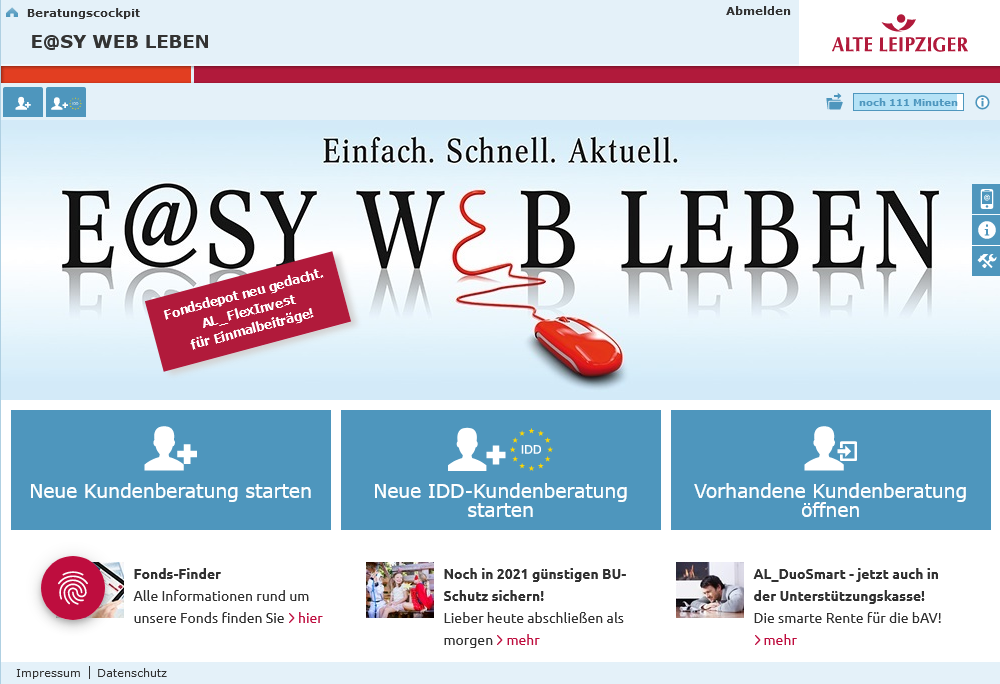
\includegraphics[width=0.8\columnwidth]{images/Easy_Web_Leben_allgemein.png}
\caption{Die Startseite von Easy Web \cite{easy_web}: Es können Kundenprofile zur Kalkulation verschiedener Altersvorsorgeprodukte angelegt und gespeichert werden. Zudem besteht die Möglichkeit ein Profil von Kundinnen und Kunden im Rahmen der IDD-Versicherungsvertriebsrichtlinie anzulegen. Screenshot erstellt am 15.12.2021.}
\label{fig:easyWeballg}
\end{figure}

Verschiedene Konzepte der privaten und betrieblichen Altersvorsorge stehen bei Easy Web zur Auswahl. Mittels einer Registerkarte können Nutzerinne und Nutzer von Easy Web bei einer Beratung der Kundschaft zwischen den Bereichen der privaten und betrieblichen Altersvorsorge wechseln. Für beide Bereiche steht zudem eine weitere Registerkarte bereit, die zwischen Rentenprodukten, Berufsunfähigkeitsprodukten und Risikolebensversicherungen unterscheidet. Für jede dieser Registerkarte erscheinen mehrere Tarife, die zur Kalkulation ausgewählt werden können. Der Anwendungsfall dieser Arbeit beschränkt sich auf den Bereich der betrieblichen Altersvorsorge und den Bereich der Renten- beziehungsweise \glqq Vorsorge\grqq{}-Produkte. Dies entspricht der Zahlung einer lebenslangen Altersrente, einer einmaligen Kapitalauszahlung oder einer Mischung aus den beiden zuvor genannten Varianten bei Erreichen des vordefinierten Rentenalters. Abbildung \ref{fig:easyWebAuswahl} zeigt das Auswahlmenü für den Fall der bAV.

\begin{figure}[!htb]
\centering
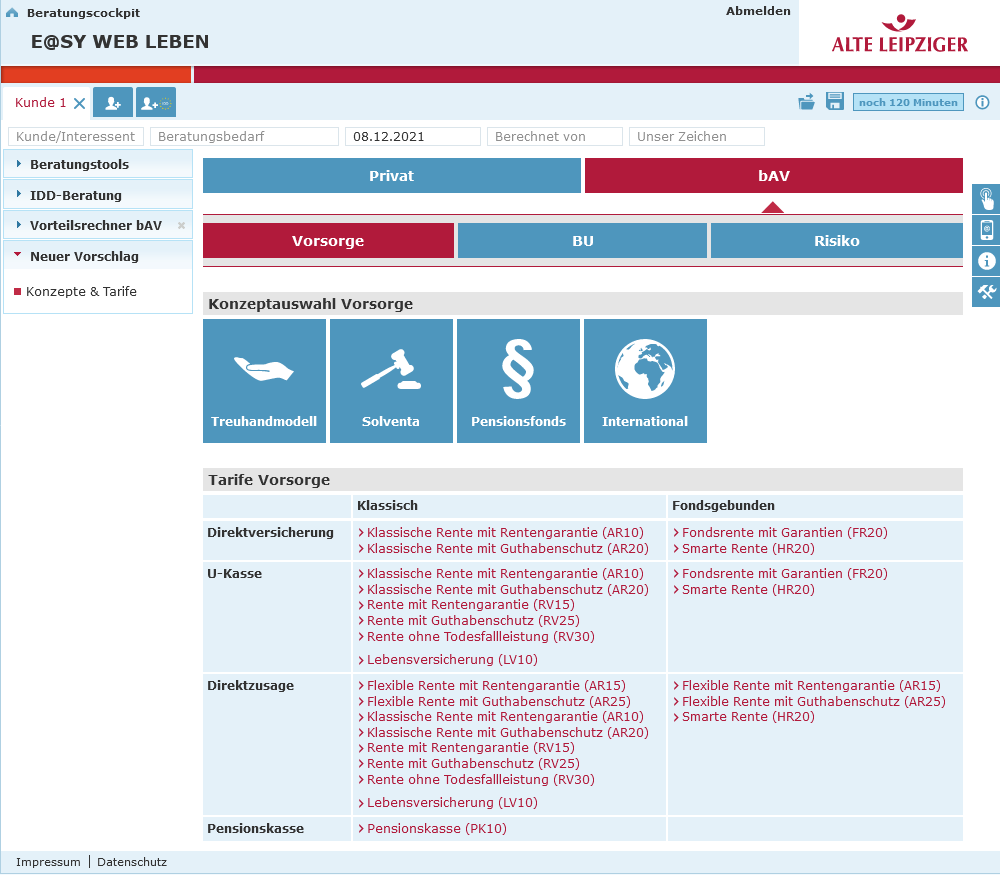
\includegraphics[width=0.7\columnwidth]{images/Easy_Web_Leben_Auswahl.png}
\caption{Das Auswahlmenü von Easy Web bei einer Kund*innenberatung: Es wird zwischen privater und betrieblicher Altersvorsorge unterschieden, zudem können Tarife verschiedener Durchführungswege ausgewählt werden. Screenshot erstellt am 15.12.2021.}
\label{fig:easyWebAuswahl}
\end{figure}

Easy Web ermöglicht die Auswahl von Produkten der bAV über vier der fünf möglichen Durchführungswege (vgl. \autoref{subsec:versicherungsgrundlagen}), die je nach Wahl des Durchführungsweges über eines der verbundenen Unternehmen der ALH-Gruppe abgewickelt werden \cite{alh_bav}. Die folgenden Ausführungen fassen die Durchführungswege und ihre Abwicklung innerhalb der ALH-Gruppe zusammen. Dabei gilt es zu berücksichtigen, dass Easy Web bzw. die ALH-Gruppe die Durchführungswege intern in einer anderen Art und Weise zuordnet als im allgemeinen Gebrauch: Easy Web unterscheidet im Bereich der Durchführungswege lediglich zwischen Direktversicherung, Pensionskasse und Direktzusage und führt zusätzlich den Parameter \glqq Art der Rückdeckung\grqq{} ein. Dieser kann die Werte \glqq keine\grqq{}, \glqq Unterstützungskasse\grqq{} oder \glqq Rückdeckungsversicherung\grqq{} annehmen.
\begin{itemize}
\item Direktversicherung / keine Rückdeckung: Abgewickelt über die Alte Leipziger Lebensversicherung a.G.
\item Direktzusage / Unterstützungskasse: Abgewickelt über die Alte Leipziger Unterstützungskasse e.V., rückdeckungsversichert über die Alte Leipziger Lebensversicherung a.G.
\item Direktzusage / Rückdeckungsversicherung: Abgewickelt über die Alte Leipziger Lebensversicherung a.G. als Rückdeckungsversicherung für eine Direktzusage eines Unternehmens.
\item Pensionskasse / keine Rückdeckung: Abgewickelt über die Alte Leipziger Pensionskasse AG
\end{itemize} 

Bei der Wahl der Anlagestrategie der Beiträge der Kundschaft und damit unmittelbar auch der garantierten Leistungen existieren im Bereich der Altersvorsorge die Varianten der klassischen, fondsgebundenen und hybriden Tarife. Bei klassischen Tarifen wird das Guthaben der Kundinnen und Kunden einzig im Deckungskapital des Versicherers angelegt \cite{alh_produkte}. Bei fondsgebundenen Tarifen werden die Beiträge hingegen in Investmentfonds investiert und unterliegen somit den Schwankungen des Kapitalmarktes \cite{alh_produkte}. Hybride Tarife vereinen die beiden Varianten der klassischen und fondsgebundenen Tarife und setzen auf mehrere Töpfe in der Anlage der Beiträge der Kundschaft \cite{alh_produkte}. Im Bereich der bAV vertreibt die ALH-Gruppe keine Produkte mit reiner Fondsanlage, sondern bezeichnet Produkte mit hohem Anteil in der Fondsanlage und zusätzlichen Garantiekomponenten als fondsgebundene Produkte \cite{alh_produkte}. Diese Produkte werden in der Eingabemaske von Easy Web auch als fondsgebunden angezeigt (vgl. Abbildung \ref{fig:easyWebAuswahl}). 

Im folgenden werden die verschiedenen Tarife vorgestellt, welche bei Easy Web ausgewählt werden können. Die Erläuterungen basieren auf \cite{alh_produkte}:
\begin{itemize}
\item Rente mit Rentengarantie (RV15) / mit Guthabenschutz (RV25) / ohne Todesfallleistung (RV30): Als Variante der klassischen Tarife wandern die Beiträge der Versicherten bei diesen Tarifen vollständig in das Deckungskapital der Alten Leipziger Lebensversicherung a. G. und werden zudem mit einem Rechnungszins vollständig garantiert. Zusätzlich bestimmt die Wahl des Tarifs zusätzliche Bausteine im Todesfall des Leistungsempfängers: Bei Wahl der Rentengarantie wird ein bestimmtes Alter der versicherungsnehmenden Person bestimmt oder eine bestimmte Dauer ab Rentenbeginn festgelegt, bis zu welchem die Rente auch im Todesfall an Hinterbliebene weiterhin ausbezahlt wird. Bei Wahl des Guthabenschutzes wird das verbleibende Guthaben nach Abzug der bereits gezahlter Renten an Hinterbliebene ausbezahlt. Die dritte Variante verzichtet auf jegliche Leistungen im Todesfall. Diese drei Tarife können bei Easy Web nur über die Durchführungswege der Direktzusage / Rückdeckungsversicherung oder Direktzusage / Unterstützungskasse ausgewählt werden.
\item Moderne klassische Rente mit Rentengarantie (AR10) / mit Guthabenschutz (AR20): Die Tarife AR10 und AR20 gleichen in ihrer Anlagestruktur der Tarife RV15, RV25 und RV30. Die Beiträge werden im Deckungsstock in sichere Kapitalanlagen investiert und werden für die Rentenbezugszeit garantiert. Die moderne klassische Rente basiert auf einem niedrigeren Garantiezins als die Tarife RV15, RV25 und RV30 und ermöglicht zudem eine flexible Gestaltung der Beitragshöhe. Der Todesfallschutz (mit Guthabenschutz / Rentengarantie) der modernen klassischen Rente gleicht den korrespondierenden Varianten der Tarife RV15 und R25. Die moderne klassische Rente ist in Easy Web über die Durchführungswege Direktversicherung, Direktzusage / Rückdeckungsversicherung und Direktzusage / Unterstützungskasse verfügbar.
\item Pensionskasse (PK10): Dieser Tarif ist der einzige Tarif, der in Easy Web über den Durchführungsweg der Pensionskasse zur Verfügung steht. Er gleicht in seiner Anlagestruktur der modernen klassischen Rente mit Rentengarantie. Im Allgemeinen unterscheiden sich die beiden Tarife PK10 und AR10 kaum, die wesentliche Ausnahme bildet dabei die Abwicklung des Tarifs über die Pensionskasse im Falle des Tarifs PK10 und über die Lebensversicherungsgesellschaft im Falle des Tarifs AR10.
\item Flexible Rente mit Rentengarantie (AR15) / mit Guthabenschutz (AR15): Die flexible Rente der ALH-Gruppe entspricht einem statischen hybriden Tarif. Kundinnen und Kunden können den Anteil des Investments in einen selbst gewählten Investmentfonds individuell spezifizieren. Der verbleibende Anteil der Beiträge wird dann im Deckungsstock angelegt und mit einem Rechnungszins garantiert. Für den Anteil der Anlage im Investmentfonds wird zudem ein Rentenfaktor garantiert. Die Tarifvarianten bezüglich des Todesfallschutzes entsprechen denen der modernen klassischen Rente. Ausgewählt werden kann die flexible Rente in Easy Web nur über den Durchführungsweg Direktzusage / Rückdeckungsversicherung.
\item Fondsrente mit Garantien (FR20): Die Fondsrente mit Garantien ist ebenfalls ein hybrider Tarif, der im Gegensatz zu den Tarifen AR15 und AR25 einem \glqq dynamischen 3-Topf-Modell\grqq{} entspricht. Die Anlage der Beiträge setzt sich hier aus dem klassischen Sicherungsvermögen im Deckungsstock des Versicherers, einem Wertsicherungsfonds und einem zusätzlichen individuell gewählten Investmentfonds zusammen. Die Beiträge werden dabei auf die drei verschiedenen Töpfe dynamisch während der Laufzeit aufgeteilt, sodass das Gesamtguthaben eine Verlustobergrenze in vordefinierten Zeiträumen nicht überschreitet. Das Gesamtguthaben der Kundinnen und Kunden wird bis zu einem vordefinierten Grad garantiert. Im Todesfall des Bezugsberechtigten der Rente besitzt der Tarif eine Rentengarantie mit Rentengarantiezeit. Die Fondsrente ist in Easy Web via Direktversicherung und Direktzusage / Unterstützungskasse verfügbar.
\item Smarte Rente (HR20): Die smarte Rente entspricht ebenfalls einem dynamischen hybriden Tarif, der jedoch lediglich auf zwei Anlagetöpfe setzt. Neben der Anlage im Deckungsstock werden die Beiträge lediglich in einen Investmentfonds investiert, der von der ALH-Gruppe vorgeben ist. Zudem unterscheidet sich die smarte Rente gegenüber der Fondsrente derart, dass bei der smarten Rente das Vertragsguthaben vor Rentenbeginn in den Deckungsstock umgeschichtet wird, sodass das garantierte Kapital des Vertrages zu Rentenbeginn sichergestellt ist. Die möglichen Durchführungswege der smarten Rente sind die Direktversicherung, die Unterstützungskasse und die Direktzusage. Auch die smarte Rente besitzt eine Rentengarantie mit Rentengarantiezeit im Todesfall. Wie die moderne klassische Rente kann die smarte Rente bei Easy Web über die Durchführungswege Direktversicherung, Direktzusage / Rückdeckungsversicherung und Direktzusage / Unterstützungskasse ausgewählt werden.
\end{itemize}

Wählt man nun einen der zur Verfügung stehenden Tarife aus, öffnet sich eine Eingabemaske zur Eingabe verschiedener Parameter, welche zur Rentenkalkulation zur Rate gezogen werden. Neben Angaben zur versicherten Person müssen Nutzer*innen von Easy Web zudem Informationen zum gewählten Tarif, eventuellen Zusatzversicherungen und der optionalen Beitragsdynamik angeben. Darüber hinaus werden je nach Wahl des Tarifs und Durchführungsweges detaillierte Angaben zum Versicherungsschutz verlangt: Dies umfasst bei allen Tarifen den Versicherungsbeginn, die Art der Finanzierung, die Höhe des Beitrags, das Renteneintrittsalter und die Periodizität der Beitragszahlungen. Ein weiteres Fenster unter der Bezeichnung \glqq Details\grqq{}, das jedoch nur bei bestimmten Tarifen angezeigt wird, erlaubt zudem die Angabe zusätzlicher detaillierter Faktoren: So können dort beispielsweise Zuzahlungen zu Beginn des Vertragsabschlusses (bei den Durchführungswegen Direktversicherung, Pensionskasse, Direktzusage) oder die genutzten Freibeträge im Sinne von § 3 Nr. 63 EStG und § 40 b EStG (bei den Durchführungswegen Pensionskasse und Direktversicherung, vgl. \autoref{subsec:versicherungsgrundlagen}) spezifiziert werden. Abbildung \ref{fig:easyWebEingabe} zeigt die Eingabemaske beispielhaft für den Tarif \glqq Klassische Rente mit Rentengarantie (AR10)\grqq{} des Durchführungswegs Direktversicherung.

\begin{figure}[!h]
\centering
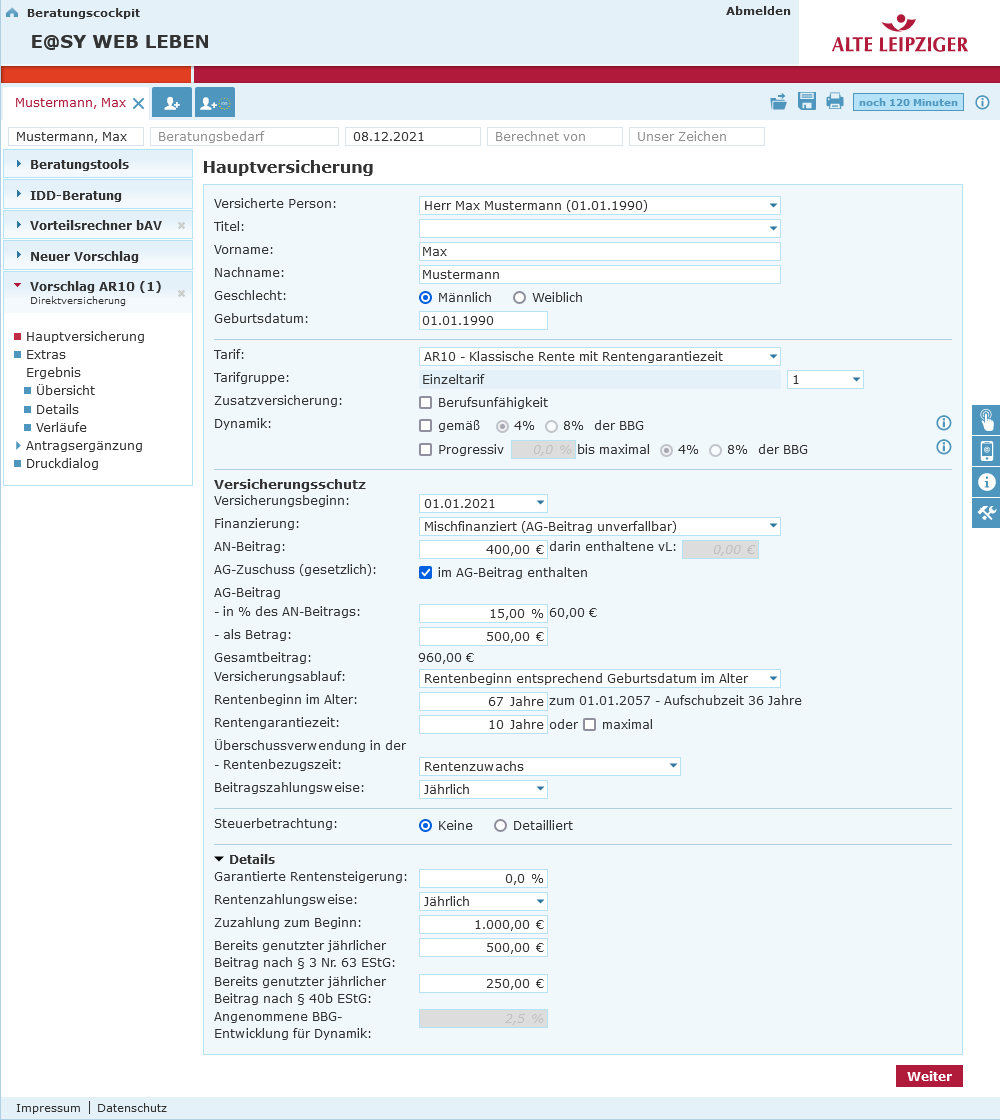
\includegraphics[width=0.72\columnwidth]{images/Easy_Web_Eingabe.png}
\caption{Die Eingabemaske für den Tarif \glqq Klassische Rente mit Rentengarantie (AR10)\grqq{} des Durchführungswegs Direktversicherung. Im oberen Bereich werden Angaben zur versicherten Person verlangt, darunter folgt die Spezifizierung der Parameter für den Tarif. Screenshot erstellt am 15.12.2021.}
\label{fig:easyWebEingabe}
\end{figure}

Nach Ausfüllen dieser einführenden Eingabemaske zur Angebotserstellung führt Easy Web Nutzer*innen durch weiterführende Formularfelder: Diese können unter anderem die Spezifizierung der Zusatzversicherungen oder die Wahl der Kapitalanlage bei fondsgebundenen Tarifen sein. Anschließend berechnet Easy Web ein Ergebnis für die garantierte und zu erwartende Rente. 

Fehlerhafte Eingaben werden von Easy Web als solche in den meisten Fällen erst beim Aufruf der Ergebnisseite angezeigt. Dies können einerseits Fehler bezüglich der Daten der Kundinnen und Kunden wie ein fehlendes Geburtsdatum sein, andererseits Fehler bezüglich der Werte zum Versicherungsschutz. In beiden Fällen verweist Easy Web auf die Haupteingabemaske zurück und zeigt den konkreten Eingabefehler an. Abbildung \ref{fig:easyWebFehler} zeigt eine beispielhafte Fehlermeldung im Falle einer Eingabe eines jährlichen Beitrags von 0 Euro für den Tarif AR10 und den Durchführungsweg der Direktversicherung.

\begin{figure}[!htb]
\centering
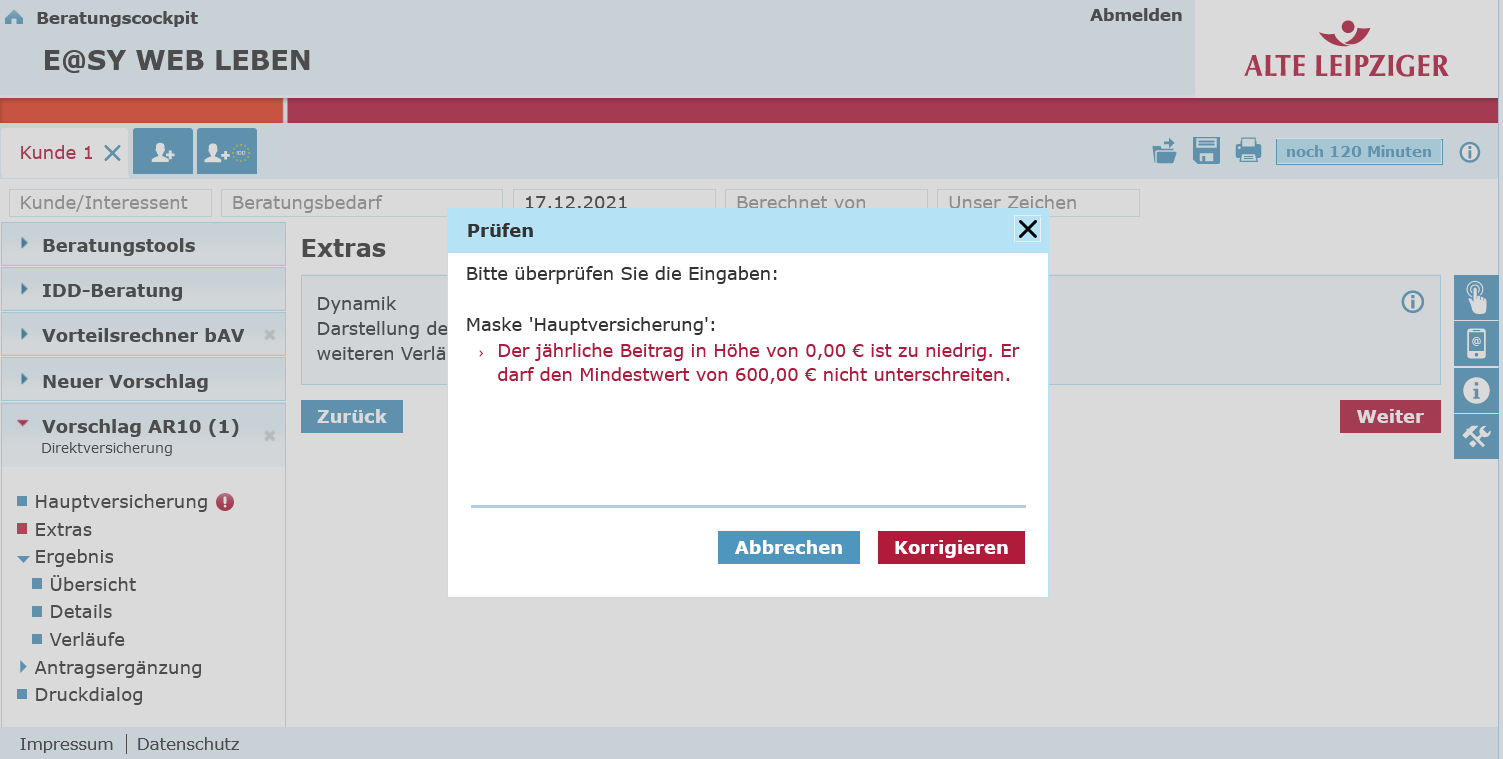
\includegraphics[width=0.8\columnwidth]{images/Easy_Web_Fehler.png}
\caption{Fehlermeldung von Easy Web bei einer Eingabe des Beitrags von 0 Euro im Tarif AR10 des Durchführungswegs Direktversicherung. Screenshot erstellt am 15.12.2021.}
\label{fig:easyWebFehler}
\end{figure}

\section{Implementierung}\label{sec:implementierung}

Im folgenden Abschnitt wird die konkrete Umsetzung zur Beantwortung der Fragestellung dieser Arbeit vorgestellt. Der zugehörige Programmcode kann öffentlich zugänglich auf der Github-Plattform eingesehen werden \cite{github}.

Das im vorausgehenden Abschnitt erwähnte Fehlerverhalten von Easy Web steht dabei im Fokus: Anhand der Methoden des Combinatorial Testing (vgl. \autoref{sec:combinatorialTesting}) werden verschiedene Mengen an Testfällen zur Überprüfung der Plausibilität der möglichen Eingaben in Easy Web erstellt und verglichen. Dies erfolgt anhand mehrerer Ansätze, die unterschiedliche Teilfragestellungen beantworten:
\begin{enumerate}
\item Erstellung eines \glqq Basis-Systems\grqq{} mit Combinatorial Testing unter Berücksichtigung von Bedingungen des zu testenden Systems: Ist es überhaupt möglich Testfälle für ein System wie Easy Web mittels Combinatorial Testing zu erstellen?
\item Vergleich Combinatorial Testing / Random Testing: Schafft Combinatorial Testing Vorteile gegenüber einem zufälligen Testverfahren?
\item Erweiterung des \glqq Basis-Systems\grqq{} zu einem 'Erweiterten System': Inwieweit verändert die Einführung komplexerer Parameterstrukturen -- im Speziellen die Einführung der Finanzierungsart und separate Parameter für Arbeitgeber- und Arbeitnehmerbeitrag -- die Resultate im Vergleich zum einfacheren 'Basis-System'?
\item $t$-fache Kombinatorik für jeden Durchführungsweg: Ist es sinnvoll spezifische Parameter zu extrahieren -- im Speziellen die Kombinationen der Durchführungswege und der Art der Rückdeckung -- und für deren Werte jeweils unabhängig voneinander Testmengen mittels Combinatorial Testing zu erstellen?
\item Vergleich verschiedener Combinatorial Testing Tools / Algorithmen: Welcher Algorithmus beziehungsweise welches Tool ist für die praktische Anwendung am nützlichsten?
\end{enumerate}

Als Grundlage aller Untersuchungen dienen die \glqq Vorsorge-Tarife\grqq{} der bAV in Easy Web, wie sie in Abbildung \ref{fig:easyWebAuswahl} zu erkennen sind. Der Tarif der Lebensversicherung (LV10) wird im Anwendungsfall nicht berücksichtigt. 

Der Anwendungsfall bezieht sich aus Gründen der Übersichtlichkeit auf eine reduzierte Auswahl der möglichen Eingabeparameter der verschiedenen Tarife in der Eingabemaske von Easy Web (vgl. \autoref{fig:easyWebEingabe}): Angaben zur versicherten Person werden im Rahmen dieser Arbeit fest vorgegeben und sind nicht variabel, ebenso Parameter optionaler Zusatzversicherungen \footnote{Verwendete Ausprägungen der Parameter zur versicherten Person und optionaler Zusatzversicherung: Max Mustermann, männlich, geb. 01.01.1980, keine Zusatzversicherung, keine Dynamik}. Außerdem werden eine progressive Beitragsentwicklung und jegliche Parameter zur Rentenauszahlung wie Rentenbeginn oder etwaige Todesfallleistungen ausgeschlossen. Letztere Annahme führt dazu, dass für die Tarife AR10 / AR20, AR15 / AR25, RV15 / RV25 / RV30 im Rahmen dieser Arbeit jeweils keine Unterschiede existieren und diese deshalb im Sinne einer Äquivalenzklassenbildung (vgl. \autoref{subsub:äquivalenklassenmethode}) zusammengefasst werden: AR10 / AR20 wird im Folgenden als AREven bezeichnet, AR15 / AR25 als AROdd und RV15 / RV25 / RV30 als RVx. 

Weitere Annahmen an das im Anwendungsfall untersuchte System sind: Die Beitragszahlung zur bAV erfolgt jährlich mit einem beliebigen, aber festen Beitrag. Dabei wird angenommen, dass die Arbeitgeberzulage stets 0\% beträgt. Der Versicherungsbeginn wird auf den 01.01.2021 festgesetzt, der Rentenbeginn soll stets am 01.01. eines Jahres erfolgen. Dies bewirkt, dass das Versicherungsjahr dem Kalenderjahr entspricht und infolgedessen sich alle Beitragsgrößen auf das Kalenderjahr beziehen.


\subsection{Basis-System}\label{subsec:ImplBasisModell}

Aus den getroffenen Annahmen ergibt sich ein zu testendes System aus verschiedenen Parametern, welches als Grundlage der Untersuchungen dieser Arbeit dient. Dieses Testsystem wird im Folgenden als \glqq Basis-System\grqq{} bezeichnet. Das Basis-System umfasst sieben verschiedene Parameter und 25 Bedingungen, die berücksichtigt werden müssen. Die Bedingungen umfassen Tarifvarianten in Abhängigkeit des Durchführungswegs und der Art der Rückdeckung und Vorgaben in Bezug auf die Wahl der möglichen Werte für die verschiedenen Parameter. Konkrete Beispiele werden dazu in den folgenden Absätzen aufgeführt, zudem kann die vollständige Liste der Bedingungen im Anhang dieser Arbeit nachgelesen werden (vgl. \autoref{sec:bedingungenSimple}). \autoref{tab:sutSimple} zeigt einen Überblick über die verschiedenen Parameter des Basis-Systems und die zugehörigen möglichen Werte.

\begin{table}[htb!]
\footnotesize
\begin{tabularx}{\textwidth}{|X|l|}
\hline
\cellcolor{grauinfo}Parameter                                      & \cellcolor{grauinfo}Mögliche Werte                                       \\ \hline
Durchführungsweg                               & Direktversicherung, Direktzusage, Pensionskasse      \\ \hline
Art der Rückdeckung\footnotemark               & keine, Rückdeckungsversicherung, Unterstützungskasse \\ \hline
Tarif                                          & AREven, AROdd, FR20, HR20, PK10, RVx                 \\ \hline
Beitrag                                        & 0, 24, 299, 599, 600, 5.000, 125.001                 \\ \hline
Zuzahlung zu Beginn                            & 0, 99, 299, 2.000, 5.001, 1.000.001                  \\ \hline
bereits genutzter Beitrag nach § 40 b EStG     & 0, 2.148, 2.149                                      \\ \hline
bereits genutzter Beitrag nach § 3 Nr. 63 EStG & 0, 2.068, 4.068                                      \\ \hline
\end{tabularx}
\normalsize
\caption{Die Parameter und möglichen Werte des Basis-Systems}
\label{tab:sutSimple}
\end{table}
\footnotetext{Die Ausprägung der Unterstützungskasse wird in der Literatur üblicherweise als eigener Durchführungsweg betrachtet (vgl. dazu \autoref{subsec:versicherungsgrundlagen}). Easy Web ordnet die Unterstützungskasse intern dem Durchführungsweg Direktzusage zu und führt sie als mögliche Art der Rückdeckung.} 

Das Basis-System unterscheidet nicht zwischen den verschiedenen Finanzierungsarten der bAV: Als Vereinfachung wird angenommen, dass nur ein einziger Wert als Beitragshöhe existiert. Dies bedeutet im Konkreten: Falls die modellierte Rente Arbeitgeber-finanziert / Arbeitnehmer-finanziert ist, fällt der gewählte Beitrag vollständig dem Arbeitgeber / dem Arbeitnehmer zu. Falls die Rente Misch-finanziert ist, soll der Beitrag zur Hälfte auf beide Parteien aufgeteilt werden. Eine detaillierte Betrachtungsweise der Finanzierungsart wird im Erweiterten System (vgl. \autoref{subsec:ImplErweitertesModell}) aufgegriffen, wobei ebenfalls stets absolute Beiträge als Basis dienen. Im Kontext der Misch-Finanzierung werden daher relative Arbeitgeber-Anteile ausgeschlossen.

Für die Parameter Durchführungsweg, Art der Rückdeckung und Tarif entsprechen die möglichen Werte des Basis-System den Auswahlmöglichkeiten des Auswahlmenüs im Bereich \glqq Vorsorge\grqq{} der bAV bei Easy Web (vgl. \autoref{fig:easyWebAuswahl}). Einzige Ausnahme: Der Tarif LV10 wird ausgeschlossen.

Die möglichen Werte für Beitragshöhe, Zuzahlung zu Beginn, bereits genutzter Beitrag nach § 40 b EStG und bereits genutzter Beitrag nach § 3 Nr. 63 EStG ergeben sich aus einer Analyse des Fehlerverhaltens von Easy Web. Durch wiederholte Experimente bei der Nutzung von Easy Web und einer Analyse der Produktinformationen \cite{alh_produkte} wurden untere und obere Schranken für die Höhe der Beiträge ermittelt, die Easy Web als Fehlergrenzen betrachtet. \autoref{tab:beitragsgrenzen} zeigt die Auflistung der Beitragsgrenzen in Abhängigkeit des Durchführungswegs, der Art der Rückdeckung und der zugehörigen Tarife. In roter Farbe sind die unteren Schranken aufgeführt, in grüner Farbe die oberen Schranken.

% Please add the following required packages to your document preamble:
% \usepackage{multirow}
% \usepackage{graphicx}
% Please add the following required packages to your document preamble:
% \usepackage{multirow}


% Please add the following required packages to your document preamble:
% \usepackage{multirow}


% Please add the following required packages to your document preamble:
% \usepackage{multirow}
% Please add the following required packages to your document preamble:
% \usepackage{multirow}


\renewcommand{\arraystretch}{2.5}

\begin{table}[!htb]
\scriptsize
\begin{tabular}{|M{\durchfuehrungsweg}|M{\finanzierung}|M{\tarife}|M{\beitrag}|M{\zuzahlung}|M{\bvierzig}|M{\bdreiEStG}|}
\hline
\cellcolor{grauinfo}Durchführungs- weg / Art der Rückdeckung &
  \cellcolor{grauinfo}Finanz- ierung &
  \cellcolor{grauinfo}Tarife &
  \cellcolor{grauinfo}Beitrag &
  \cellcolor{grauinfo}Zuzahlung &
  \cellcolor{grauinfo}Verw. Beitrag § 40 b &
  \cellcolor{grauinfo}Verw. Beitrag § 3(63) \\ \hline
\multirow{2}{=}{\centering Direkt- versicherung / keine} &
  \multirow{2}{=}{\centering \textit{AN, AG, Misch}} &
  \multirow{2}{=}{\centering AREven, HR20, FR20} &
  \multicolumn{1}{M{\beitrag}|}{\textcolor{red2}{$\geq$ 600}} &
  \multicolumn{1}{M{\zuzahlung}|}{\textcolor{red2}{= 0 bzw. $\geq$ 100}} &
  \multicolumn{2}{M{\bZwei}|}{\textcolor{red2}{$\geq$ 0}} \\ \cline{4-7} 
 &
   &
   &
  \multicolumn{4}{M{\bAlle}|}{\textcolor{modGreen}{Summe aller Beiträge $\leq$ 6.816   (BBG-Grenze) \& Beitrag 40b $\leq$ 2.148}} \\ \hline


\multirow{2}{=}{\centering Pensionskasse / keine} &
  \multirow{2}{=}{\centering \textit{AN, AG, Misch}} &
  \multirow{2}{=}{\centering PK10} &
  \multicolumn{1}{M{\beitrag}|}{\textcolor{red2}{$\geq$ 300}} &
  \multicolumn{1}{M{\zuzahlung}|}{\textcolor{red2}{= 0 bzw. $\geq$ 300}} &
  \multicolumn{2}{M{\bZwei}|}{\textcolor{red2}{$\geq$ 0}} \\ \cline{4-7} 
 &
   &
   &
  \multicolumn{4}{M{\bAlle}|}{\textcolor{modGreen}{Summe aller Beiträge $\leq$ 6.816   (BBG-Grenze) \& Beitrag 40b $\leq$ 2.148}} \\ \hline

\multirow{6}{=}{\centering Direktzusage / Unterstütz- ungskasse} &
  \multirow{6}{=}{\centering \textit{AN, AG}} &

  \multirow{2}{=}{\centering AREven, HR20} &
  \multicolumn{1}{M{\beitrag}|}{\textcolor{red2}{$\geq$ 600}} &
  \multicolumn{3}{M{\bDrei}|}{\multirow{6}{=}{\centering \vspace{-1cm}\hspace{-0.8cm}--}} \\ \cline{4-4}
 &
   &
   &
  \multicolumn{1}{M{\beitrag}|}{\textcolor{modGreen}{$\leq$ 125.000 (Verweis auf Direktionsanfrage)}} &
  \multicolumn{3}{l|}{} \\ \cline{3-4} 
  &
  &
\multirow{2}{=}{\centering FR20} &
  \multicolumn{1}{M{\beitrag}|}{\textcolor{red2}{$\geq$ 300}} &
  \multicolumn{3}{l|}{} \\ \cline{4-4}
&
&
&
  \multicolumn{1}{M{\beitrag}|}{\textcolor{modGreen}{$\leq$ 125.000 (Verweis auf Direktionsanfrage)}} &
  \multicolumn{3}{l|}{} \\ \cline{3-4} 
&
&
\multirow{2}{=}{\centering RVx} &
  \multicolumn{1}{M{\beitrag}|}{\textcolor{red2}{$\geq$ 25 \& wie bei Rückdeckungsversicherung / RVx}} &
  \multicolumn{3}{l|}{} \\ \cline{4-4}
&
&
&
  \multicolumn{1}{M{\beitrag}|}{\textcolor{modGreen}{$\leq$ 125.000 (Verweis auf Direktionsanfrage)}} &
  \multicolumn{3}{l|}{} \\ \hline

%%

\multirow{4}{=}{\centering Direktzusage / Rückdeckungs- versicherung} &
  \multirow{4}{=}{\centering \textit{AG}} &
  \multirow{2}{=}{\centering AREven, AROdd,   HR20} &
  \multicolumn{1}{M{\beitrag}|}{\textcolor{red2}{$\geq$ 600}} &
  \multicolumn{1}{M{\zuzahlung}|}{\textcolor{red2}{$\geq$ 0}} &
  \multicolumn{2}{M{\bZwei}|}{\multirow{4}{=}{\centering  \vspace{-0.5cm}\hspace{-0.4cm}--}} \\ \cline{4-5}
 &
   &
   &
  \multicolumn{1}{M{\beitrag}|}{\textcolor{modGreen}{$\leq$   125.000 (Verweis auf Direktionsanfrage)}} &
  \multicolumn{1}{M{\zuzahlung}|}{\textcolor{modGreen}{$\leq$ 1 Mio.}} &
  \multicolumn{2}{l|}{} \\ \cline{3-5}
 &
   &
  \multirow{2}{=}{\centering RVx} &
  \multicolumn{1}{M{\beitrag}|}{\textcolor{red2}{Ergibt sich aus garantierter Rente von 600 Euro (hängt vom Alter ab)}} &
  \multicolumn{1}{M{\zuzahlung}|}{\textcolor{red2}{= 0 bzw. $\geq$ 500}} &
  \multicolumn{2}{l|}{} \\ \cline{4-5}
 &
   &
   &
  \multicolumn{1}{M{\beitrag}|}{\textcolor{modGreen}{$\leq$   125.000 (Verweis auf Direktionsanfrage)}} &
  \multicolumn{1}{M{\zuzahlung}|}{\textcolor{modGreen}{$\leq$ 5.000}} &
  \multicolumn{2}{l|}{} \\ \hline


\end{tabular}

\normalsize
\caption{Grenzen (in Euro) der möglichen Eingabewerte der Beitragsparameter in Easy Web in Abhängigkeit des Durchführungswegs, der Rückdeckung und der jeweiligen Tarife. Rot sind untere Schranken markiert, grün obere Schranken}
\label{tab:beitragsgrenzen}
\end{table}

\renewcommand{\arraystretch}{1.5}

Für die Durchführungswege Direktversicherung und Pensionskasse ergibt sich eine kombinierte oberere Schranke für Beitragshöhe, Zuzahlung zu Beginn, bereits genutzter Beitrag nach § 40 b EStG und bereits genutzter Beitrag nach § 3 Nr. 63 EStG: Die Summe dieser Parameter darf den Wert der 8\%-Fördergrenze der Beitragsbemessungsgrenze nach § 3 Nr. 63 EStG nicht überschreiten (vgl. \autoref{subsec:versicherungsgrundlagen}). Höhere Beiträge als der Wert von 6.816 Euro erlaubt Easy Web bei der Eingabe nicht. Darüber hinaus darf bei den Durchführungswegen Direktversicherung und Pensionskasse der genutzte Beitrag im Sinne von § 40 b EStG den Maximalbetrag von 2.148 Euro nicht überschreiten (vgl. \autoref{subsec:versicherungsgrundlagen}).

Für die Höhe des Beitrages existiert beim Durchführungsweg der Direktzusage eine obere Schranke, die durch den jährlichen Maximalbeitrag von 125.000 Euro festgesetzt ist. Falls dieser Wert überschritten wird, berechnet Easy Web keine Rente und zeigt eine Fehlermeldung mit einem Verweis auf eine notwendige Direktionsanfrage an. Für die untere Schranke gilt für die Tarife der klassischen RVx-Rente eine besondere Regelung: Die Untergrenze ergibt sich dabei aus einer garantierten jährlichen Rente von 600 Euro, die sich über die Faktoren der Beitragshöhe und der Dauer der Beitragszahlungen (beziehungsweise dem Alter der versicherten Person) ermitteln lässt.

Die bereits genutzten Beiträge nach § 40 b EStG und nach § 3 Nr. 63 EStG spielen aufgrund der gesetzlichen Regelungen nur für die Durchführungswege Direktversicherung und Pensionskasse eine Rolle, eine Zuzahlung ermöglicht Easy Web lediglich beim Durchführungsweg Direktzusage und der Rückdeckung via Rückdeckungsversicherung. In diesen Fällen wird durch Bedingungen an das zu testende System der Wert 0 für die ausgeschlossenen Parameter festgesetzt. So gilt als Beispiel für die Kombination Direktzusage / Rückdeckungsversicherung: \textit{Durchführungsweg = 'Direktzusage' \&\& Art der Rückdeckung = 'Rückdeckungsversicherung' $\Rightarrow$ Verw. Beitrag § 40 b = 0 \&\& Verw. Beitrag § 3(63) = 0.}

Darüber hinaus setzt Easy Web in bestimmten Fällen eine Mindestanforderung an die Höhe der Zuzahlung voraus: Die Zuzahlung bei den Kombinationen Direktversicherung / keine Rückdeckung, Pensionskasse / keine Rückdeckung und Direktzusage / Rückdeckungsversicherung / RVx muss entweder gleich 0 sein oder einen Mindestbetrag überschreiten (vgl. \autoref{tab:beitragsgrenzen}).

\hspace{1cm}Die konkreten Werte für Beitragshöhe, Zuzahlung zu Beginn, bereits genutzter Beitrag nach § 40 b EStG und bereits genutzter Beitrag nach § 3 Nr. 63 EStG wurden anhand der Analyse aus \autoref{tab:beitragsgrenzen} und den Methoden der Äquivalenzklassenbildung (vgl. \autoref{subsub:äquivalenklassenmethode}) und Grenzwertanalyse (vgl. \autoref{subsub:grenzwertanalyse}) ermittelt. Für jede Schranke des Systems wurden Äquivalenzklassen oberhalb und unterhalb der Schranke angenommen und darauf aufbauend mindestens ein Wert pro Klasse in das Testsystem aufgenommen. Dies gilt insbesondere auch für kombinierte Schranken mehrerer Parameter wie die 8\%-Fördergrenze der Beitragsbemessungsgrenze nach § 3 Nr. 63 EStG. Zudem wurden im Besonderen die Grenzwerte im Sinne der Grenzwertanalyse betrachtet, sodass pro Äquivalenzklasse die betroffenen Schranken möglichst exakt getroffen werden. Beispiel hierfür sind die Werte 2.148 Euro und 2.149 Euro für den bereits genutzten Beitrag nach § 40 b EStG. 

Die aus diesem Vorgehen resultierenden Werte für die verschiedenen Beitragsparameter sind in \autoref{tab:äquivalenzklassenSimple} dargestellt. Dabei gilt es zu berücksichtigen, dass nicht alle Werte der Beitragsparameter, die in \autoref{tab:sutSimple} aufgeführt sind, für alle Durchführungswege relevant sind: Durch zusätzliche Bedingungen an das Testsystem werden bei der Erstellung der Testmengen lediglich die in \autoref{tab:äquivalenzklassenSimple} aufgeführten Werte für die Kombinationen der Durchführungswege, Art der Rückdeckung und Tarife bei der Erstellung der Testfälle berücksichtigt. Beispielsweise gilt für die Kombination Direktversicherung / keine Rückdeckung bei allen Tarifen folgende Bedingung: \textit{Durchführungsweg = 'Direktversicherung' $\Rightarrow$ Beitrag = 0 || Beitrag = 599 || Beitrag = 600.}


\renewcommand{\arraystretch}{2.5}

\begin{table}[htb!]
\scriptsize
\begin{tabular}{|M{\durchfuehrungsweg}|M{\durchfuehrungsweg}|M{\zuzahlung}|M{\zuzahlung}|M{\zuzahlung}|M{\zuzahlung}|}
\hline
\cellcolor{grauinfo}Durchführ- ungsweg / Art der Rückdeckung &
  \cellcolor{grauinfo}Tarife &
  \cellcolor{grauinfo}Beitrag &
  \cellcolor{grauinfo}Zuzahlung &
  \cellcolor{grauinfo}Verw. Beitrag §~40~b &
  \cellcolor{grauinfo}Verw. Beitrag §~3~\#63 \\ \hline
  Direktversicherung &
  AREven,   HR20, FR20 &
  0,   599, 600 &
  0,   99, 2.000 &
  0,   2.148, 2.149 &
  0,   2.068, 4.068  \\ \hline

	Pensionskasse &
	 PK10 &
	  0,   299, 599, 600 &
	  0,   299, 2.000 &
	  0,   2.148, 2.149 &
	  0,   2.068, 4.068  \\ \hline

\multirow{3}{=}{\centering Direktzusage / Unterstütz- ungskasse} &
  AREven,   HR20 &
  0,   599, 600, 125.001 &
  \multicolumn{3}{M{\bDrei}|}{\multirow{3}{=}{\centering  \vspace{-0.7cm}\hspace{-1.4cm}--}} \\ \cline{2-3}

   &
  FR20 &
  0,   299, 600, 125.001 &
  \multicolumn{3}{l|}{} \\ \cline{2-3}

   &
  RVx &
  0,   24, 299, 600, 125.001 &
  \multicolumn{3}{l|}{} \\ \hline

%%

\multirow{2}{=}{\centering Direktzusage / Rückdeckungs- versicherung} &
  AREven, AROdd,   HR20 &
  0, 599, 600, 125.001 &
  0, 2.000, 1.000.001 &
  \multicolumn{2}{M{\bZwei}|}{\multirow{2}{=}{\centering  \vspace{-0.7cm}\hspace{-1.4cm}--}} \\ \cline{2-4}

   &
  RVx &
  0,   24, 299, 5.000, 125.001 &
  0, 299, 2.000, 5.001 &
  \multicolumn{2}{l|}{} \\ \hline


\end{tabular}

\normalsize
\caption{Mögliche Werte für die verschiedenen Beitragsparameter für das Basis-System in Abhängigkeit des Durchführungswegs, der Art der Rückdeckung und des Tarifs.}
\label{tab:äquivalenzklassenSimple}
\end{table}

\renewcommand{\arraystretch}{1.5}

Das vorgestellte Basis-System dient als Grundlage zur Erstellung einer Menge an Testfälle im Sinne von Combinatorial Testing (vgl. \autoref{sec:combinatorialTesting}). Für die Beantwortung der grundsätzlichen Fragestellung dieser Arbeit wurden Testmengen mit einem Interaktionsparameter von $t = 2$ bis $t = 6$ via ACTS (vgl. \autoref{subsub:acts}) und dem allgemeinen IPOG-Algorithmus (vgl. \autoref{subsub:ipog}) erstellt.


\subsection{Vergleich Combinatorial Testing / Random Testing}\label{subsec:ImplRandomTesting}

Die grundlegende Fragestellung, die durch Erstellung von Testmengen des Basis-Systems beantwortet wird, sollte im Weiteren durch einen Vergleich mit einer naiven, zufallsbasierten Herangehensweise erweitert werden und aufzeigen, inwieweit ein systematisches Vorgehen bei der Erstellung von Testmengen hilfreich sein kann. 

Dafür wurde ein Random Testing-Ansatz (vgl. \autoref{subsec:beispieleTests}) für das zuvor vorgestellte Basis-System implementiert: Für eine vordefinierte Anzahl $N$ an Testfällen erzeugt der implementierte Random-Testing-Algorithmus zufällige Testfälle, indem für jeden Parameter des Basis-Systems zufällig ein Wert ausgewählt wird. Der erzeugte Testfall wird dann auf Konsistenz mit den 25 Bedingungen des Basis-Systems geprüft: Falls jener Testfall die Bedingungen des Basis-Systems nicht erfüllt, wird dieser verworfen und ein neuer zufälliger Testfall erstellt. Darüber hinaus prüft der Algorithmus die Testfälle auf Duplikate und verwirft diese im Falle eines bereits existierenden Testfalls.

Als Vergleichsgrößen zum Ansatz des Combinatorial Testing dienen unter anderem Effizienzmetriken des Random Testing-Ansatzes wie die Ausführungszeit und die Anzahl der benötigten Iterationen, die zur Erstellung von $N$ Testfällen benötigt werden. In Bezug auf die Ausführungszeit gilt bei allen Untersuchungen dieser Arbeit, dass diese unter identischen Bedingungen auf derselben Maschine durchgeführt wurden. 

Als weitere Vergleichsgrößen des Random Testings wurden die Abdeckung im Sinne von Combinatorial Testing mit den Metriken der $t$-fachen-Abdeckung (vgl. \autoref{subsub:TAbdeckung}), der Variablen-Wert-Abdeckung (vgl. \autoref{subsub:variablenWert}) und der (0,75-$t$)-Vollständigkeit (vgl. \autoref{subsub:pTVollständigkeit}) geprüft für $t \in \{2,3\}$. Das Random Testing-Verfahren wurde für $N \in \{50, 100, 200, 300\}$ mit jeweils 20 Wiederholungen durchgeführt. Die Ergebnisse wurden schließlich als Mittelwert der 20 Wiederholungen berechnet.


\subsection{Erweitertes System}\label{subsec:ImplErweitertesModell}

Das Basis-System beinhaltet keine spezifische Betrachtungsweise der Finanzierungsart und einer damit verbundenen Trennung zwischen Arbeitgeber- und Arbeitnehmer-Beitrag. Das \glqq Erweiterte System\grqq{} greift diesen Aspekt auf und soll aufzeigen, inwiefern sich die Erstellung von Testmengen via Combinatorial Testing auf komplexere Systeme skalieren lässt.

Das Erweiterte System ergänzt das Basis-System durch die Parameter Finanzierungsart (Arbeitgeber-, Arbeitnehmer-, Misch-finanziert) und Arbeitnehmer- und Arbeitgeberbeitrag, der Parameter Beitrag des Basis-Systems entfällt. Das Erweiterte System besitzt folglich neun verschiedene Parameter und zusätzliche sieben Bedingungen an das Testsystem im Vergleich zum Basis-System: Neu hinzugefügte Bedingungen umfassen unter anderem bestimmte Kombinationen aus Durchführungsweg und Art der Rückdeckung, die spezifische Finanzierungsarten voraussetzen. Beispielsweise wird bei Easy Web die Kombination Direktzusage / Rückdeckungsversicherung nur als Arbeitgeber-finanzierte Variante durchgeführt. Die resultierende Bedingung lautet:\textit{ Durchführungsweg = 'Direktzusage' \&\& Art der Rückdeckung = 'Rückdeckungsversicherung' $\Rightarrow$ Finanzierungsart = 'AG-finanziert'}. Die verschiedenen Finanzierungsmöglichkeiten abhängig vom Durchführungsweg, Art der Rückdeckung und Tarif können \autoref{tab:beitragsgrenzen} entnommen werden. \autoref{tab:sutComplex} zeigt eine Übersicht über die Parameter und möglichen Werte des Erweiterten Systems.

\begin{table}[htb!]
\footnotesize
\begin{tabularx}{\textwidth}{|X|l|}
\hline
\cellcolor{grauinfo}Parameter                                      & \cellcolor{grauinfo}Mögliche Werte                                       \\ \hline
Durchführungsweg                               & Direktversicherung, Direktzusage, Pensionskasse      \\ \hline
Art der Rückdeckung                            & keine, Rückdeckungsversicherung, Unterstützungskasse \\ \hline
Tarif                                          & AREven, AROdd, FR20, HR20, PK10, RVx                 \\ \hline
\textbf{Finanzierung}								   &AG-finanziert, AN-finanziert, Misch-finanziert     \\ \hline
\textbf{AN-Beitrag}                                    & 0, 299, 599, 600, 1.500, 125.001                     \\ \hline
\textbf{AG-Beitrag }                                    & 0, 24, 299, 599, 600, 1.500, 125.001                   \\ \hline
Zuzahlung zu Beginn                            & 0, 99, 299, 2.000, 5.001, 1.000.001                  \\ \hline
bereits genutzter Beitrag nach § 40 b EStG     & 0, 2.148, 2.149                                      \\ \hline
bereits genutzter Beitrag nach § 3 Nr. 63 EStG & 0, 2.068, 4.068                                      \\ \hline
\end{tabularx}
\normalsize
\caption{Die Parameter und möglichen Werte des Erweiterten Systems: Das Erweiterte System umfasst zusätzliche Parameter bezüglich der Finanzierungsart und der Unterscheidung in Arbeitgeber- und Arbeitnehmerbeitrag}.
\label{tab:sutComplex}
\end{table}

Analog zur Ermittlung der Werte der Parameter Beitragshöhe, Zuzahlung zu Beginn, bereits genutzter Beitrag nach § 40 b EStG und bereits genutzter Beitrag nach § 3 Nr. 63 EStG im Basis-System wurden die Werte für die verschiedenen Parameter des Erweiterten Systems auf Basis der Beitragsgrenzen in \autoref{tab:beitragsgrenzen} festgesetzt. Dabei wurden wie beim Basis-System die Methoden der Äquivalenzklassenmethode (vgl. \autoref{subsub:äquivalenklassenmethode}) und Grenzwertanalyse (vgl. \autoref{subsub:äquivalenklassenmethode}) kombiniert. Eine Übersicht über die möglichen Werte der verschiedenen Parameter des Erweiterten Systems (\autoref{tab:äquivalenzklassenComplex}) und die Bedingungen des Erweiterten Systems (\autoref{sec:bedingungenComplex}) befindet sich im Anhang dieser Arbeit.

Das Erweiterte System wurde mit dem Basis-System in Bezug auf die Anzahl der erzeugten Testfälle für die Interaktionsparameter $t \in \{2,3,4,5,6\}$ verglichen, ebenfalls unter Anwendung des allgemeinen IPOG-Algorithmus (vgl. \autoref{subsub:ipog}) via ACTS (vgl. \autoref{subsub:acts}): Dabei wurde zudem untersucht, wie sich das Laufzeitverhalten durch die zusätzlichen Parameter verändert.

\subsection{$t$-fache Kombinatorik für jeden Durchführungsweg}\label{subsec:ImplFullCombinations}

Sowohl beim Basis-System als auch beim Erweiterten System sind die Parameter Durchführungsweg und Art der Rückdeckung Teil der Kombinatorik bei der Erstellung der Testfallmengen mit $t$-facher Abdeckung. Dabei kann es jedoch passieren, dass durch die Reduktion der Kombinatorik auf den Wert $t$ erwünschte Kombinationen verschiedener Parameter unberücksichtigt bleiben. \autoref{tab:erklärungFullCombination} verdeutlicht dieses Prinzip: Sei $t=2$ gegeben, dann erfüllt ein Testfall mit Tarif = 'AREven' und Beitrag = 600 bereits die notwendige 2-fach-Abdeckung für das Parameterpaar Tarif / Beitrag. In \autoref{tab:erklärungFullCombination} entspricht dies dem ersten Eintrag mit Durchführungsweg Direktversicherung ohne Rückdeckung.

\renewcommand{\arraystretch}{2}
\begin{table}[!htb]
\footnotesize
\begin{tabular}{|M{\tabOther}|M{\tabOther}|M{\tabBeitrag}|M{\tabBeitrag}|}
\hline
\cellcolor{grauinfo}Durchführungsweg & \cellcolor{grauinfo}Art der Rückdeckung & \cellcolor{grauinfo}Tarif & \cellcolor{grauinfo}Beitrag \\ \hline
Direktversicherung      & keine                     & AREven   & 600   \\ \hline
Direktzusage       & Unterstützungs- kasse & AREven    & 599    \\ \hline
Direktzusage       & Rückdeckungs- versicherung & AREven    & 125.001     \\ \hline
\end{tabular}
\normalsize
\caption{Entstehende Problematik bei Einbezug des Durchführungswegs und der Art der Rückdeckung in die $t$-fach-Kombinatorik bei der Erstellung von Testmengen: Für $t=2$ wird durch den ersten Testfall die Kombination Tarif = \glqq AREven\grqq{} / Beitrag = 600 bereits abgedeckt und somit möglicherweise nicht mehr beim Durchführungsweg Direktzusage verwendet.}
\label{tab:erklärungFullCombination}
\end{table}
\renewcommand{\arraystretch}{1.5}

Die Beitragsgrenze von 600 Euro spielt jedoch nicht nur für den Durchführungsweg der Direktversicherung eine entscheidende Rolle, sondern auch für die Direktzusage, wie \autoref{tab:beitragsgrenzen} aufzeigt: Die Kombination Tarif = 'AREven' / Beitrag = 600 ist im Beispiel in  \autoref{tab:erklärungFullCombination} bereits abgedeckt, sodass für die Direktzusage andere Wertepaare der Parameter Tarif und Beitrag bevorzugt berücksichtigt werden -- im Konkreten zunächst das Paar ('AREven' / 599), anschließend ('AREven' / 125.001). Es kann also passieren, dass für den Durchführungsweg der Direktzusage bei einem Interaktionsparameter $t=2$ eine Testmenge ohne einen einzigen Testfall mit dem Beitrag von 600 Euro erzeugt wird.

Um diesem Effekt zu begegnen, wurde ein erweiterter Ansatz zur Erstellung von Testfällen mittels Combinatorial Testing implementiert: Dieser Ansatz beinhaltet die Extrahierung der Parameter Durchführungsweg und Art der Rückdeckung und die Erstellung von Testmengen via Combinatorial Testing für jede einzelne Wertekombination dieser beiden Parameter. Dieses Vorgehen stellt sicher, dass sich die kombinatorische Entfaltung von Combinatorial Testing lediglich auf die Beitragsparameter auswirkt. Als Analogie zur Benutzeroberfläche von Easy Web entspricht dieses Vorgehen der Trennung zwischen Auswahlmenü des Durchführungsweges und der Art der Rückdeckung (\autoref{fig:easyWebAuswahl}) und der Eingabemaske (\autoref{fig:easyWebEingabe}) der jeweiligen Tarife. 

\autoref{tab:modelFullCombination} stellt die Umsetzung dieses Ansatzes modellhaft dar. Bei der Erstellung der jeweiligen Testmengen wurde das Erweiterte System als Grundlage der Implementierung gewählt, da durch die Extrahierung der beiden Parameter Durchführungsweg und Art der Rückdeckung beim Basis-System lediglich fünf Parameter verbleiben würden. Dies würde die Wertekombinationen erheblich reduzieren, insbesondere würde eine Abdeckung mit Interaktionsparameter $t \in \{5,6\}$ einer vollständigen Kombinationsabdeckung entsprechen (vgl. \autoref{subsub:VollständigeAbdeckung}).

\renewcommand{\arraystretch}{2.5}
\begin{table}[!htb]
\scriptsize
\begin{tabular}{|M{\tabTemp}|M{\tabTemp}|M{\tarife}M{\tarife}M{\tarife}M{\tarife}M{\tarife}M{\tarife}M{\tarife}|}
\hline
\cellcolor{grauinfo}Durchführungs- weg &
  \cellcolor{grauinfo}Art der Rückdeckung &
  \cellcolor{grauinfo}Tarif &
  \cellcolor{grauinfo}Finanz- ierung &
  \cellcolor{grauinfo}AN- Beitrag &
  \cellcolor{grauinfo}AG- Beitrag &
  \cellcolor{grauinfo}Zuzahl- ung zu Beginn &
  \cellcolor{grauinfo}Verw. Beitrag §~40~b &
 \cellcolor{grauinfo} Verw. Beitrag §~3~\#63 \\ \hline
Direkt- versicherung & keine                    & \multicolumn{7}{c|}{\footnotesize--- $t$-fache   Kombinationsabdeckung ---} \\ \hline
Pensionskasse      & keine                    & \multicolumn{7}{c|}{\footnotesize--- $t$-fache   Kombinationsabdeckung ---} \\ \hline
Direktzusage & Rückdeckungs- versicherung & \multicolumn{7}{c|}{\footnotesize--- $t$-fache   Kombinationsabdeckung ---} \\ \hline
Direktzusage & Unterstützungs- kasse      & \multicolumn{7}{c|}{\footnotesize--- $t$-fache   Kombinationsabdeckung ---} \\ \hline
\end{tabular}
\normalsize
\caption{Modellhafte Umsetzung des Ansatzes der separaten Erstellung von Testmengen mit $t$-fach-Abdeckung für jeden Durchführungsweg und jede Art der Rückdeckung.}
\label{tab:modelFullCombination}
\end{table}
\renewcommand{\arraystretch}{1.5}

Unter Verwendung des Erweiterten Systems verbleiben sieben verschiedene Parameter für den Ansatz der $t$-fachen Kombinatorik für jeden Durchführungsweg und jede Art der Rückdeckung. Die verschiedenen Bedingungen des Erweiterten Systems (vgl. \autoref{sec:bedingungenComplex}) wurden den jeweiligen Durchführungswegen / Arten der Rückdeckung zugeordnet und angepasst. Die Erstellung der Testfallmengen für die verschiedenen Durchführungswege / Arten der Rückdeckung erfolgte via IPOG-Algorithmus (vgl. \autoref{subsub:ipog}) und ACTS (vgl. \autoref{subsub:acts}). Anschließend wurden diese um die Werte des Durchführungswegs / der Art der Rückdeckung erweitert und aneinander gefügt.

\subsection{Vergleich verschiedener Combinatorial Testing Algorithmen}\label{subsec:ImplAlgorithmen}

Zur Beantwortung der abschließenden Teilfragestellung wurden verschiedene Tools zur Erstellung von Combinatorial Testing-Testmengen verglichen. Im Konkreten wurden die Algorithmen IPOG  (vgl. \autoref{subsub:ipog}), IPOG-F (vgl. \autoref{subsub:ipog}), PICT (vgl. \autoref{subsub:pict}) und CASA (vgl. \autoref{subsub:casa}) untersucht. Weitere von ACTS unterstützte Algorithmen (IPOG-D, IPOG-F2, PaintBall, Base Choice) erfüllen die notwendigen Anforderungen des Testsystems, wie beispielsweise die Berücksichtigung von Bedingungen, nicht und wurden an dieser Stelle ausgeschlossen. Die Anwendung von IPOG und IPOG-F erfolgte über die Benutzeroberfläche von ACTS, PICT und CASA wurden über die Kommandozeile gestartet.

Die 25 Bedingungen des Basis-Systems führen beim Algorithmus CASA dazu, dass die Standardgrößen für eine obere und untere Schranke der Anzahl an Testfällen beim Start des Algorithmus (Outer Search bei CASA, vgl. \autoref{subsub:casa}) sehr weit über der tatsächlichen, minimalen Anzahl an Testfällen liegt und der Algorithmus nicht immer terminiert. Dies erfordert die Angabe einer realistischen oberen und unteren Grenze der Anzahl der Testfälle, welche als Parameter über die Kommandozeile definiert werden können: Die Resultate der Algorithmen IPOG und PICT dienten hierfür als Referenzgrößen.

Für alle vier Algorithmen wurden Testmengen für die Interaktionsparameter $t \in \{2,3,4,5,6\}$ erstellt. Anschließend wurden die Anzahl der generierten Testfälle, die Ausführungszeit und für $t \in \{2,3,4,5\}$ die Metriken der $(t+1)$-Kombinationsabdeckung (vgl. \autoref{subsub:tPlusKAbdeckung}), der $(t+1)$-Variablen-Wert-Abdeckung (vgl. \autoref{subsub:variablenWert}) und der (0,75-($t+1$))-Vollständigkeit (vgl. \autoref{subsub:pTVollständigkeit}) ermittelt. Für den nicht-deterministischen Algorithmus CASA wurde die Erstellung der Testmenge 30-fach wiederholt und der Median der zuvor aufgeführten Metriken berechnet. Zudem wurde bei CASA für jeden Interaktionsparameter die Testmenge mit der geringsten Anzahl an erzeugten Testfällen ermittelt. Als Testsystem diente das Basis-System (vgl. \autoref{subsec:ImplBasisModell}). 

\section{Ergebnisse}\label{sec:results}

Im folgenden Abschnitt werden die Resultate der Untersuchungen zur Beantwortung der verschiedenen Teilfragestellungen dieser Arbeit vorgestellt. Die Ausführungen folgen dabei der Struktur des vorherigen Abschnitts zur Implementierung (vgl. \autoref{sec:implementierung}).

\subsection{Basis-System}\label{subsec:resultsBasisModell}

Das Basis-System (vgl. \autoref{subsec:ImplBasisModell}) mit sieben verschiedenen Parametern und 25 Bedingungen besitzt für den Fall des Pairwise-Testing (Interaktionsparameter $t=2$) 293 verschiedene Variablen-Wert-Kombinationen, die bei der Erstellung einer Testmenge abgedeckt werden müssen. \autoref{tab:variablenWertBasis} zeigt die abzudeckenden Variablen-Wert-Konstellationen für die Werte $t \in \{2,3,4,5,6\}$. Mit Erhöhung des Interaktionsparameters $t$ steigt die Anzahl der abzudeckenden Variablen-Wert-Kombinationen bis zum Wert von 3.081 für $t=5$ an. Für den Parameter $t=6$ sinkt dieser Wert auf 1.873, was sich durch den steigenden Einfluss der Bedingungen des Testsystems im Zusammenhang mit der geringer werdenden Differenz zwischen Interaktionsparameter und Anzahl der Parameter des Testsystems erklären lässt.

\renewcommand{\arraystretch}{2}
\begin{table}[!htb]
\footnotesize
\begin{tabular}{|M{0.1\textwidth}|c|}
\hline
\cellcolor{grauinfo}t & \cellcolor{grauinfo}Anzahl an Variablen-Wert-Kombinationen \\ \hline
2 & 293                                    \\ \hline
3 & 1.214                                   \\ \hline
4 & 2.617                                   \\ \hline
5 & 3.081                                   \\ \hline
6 & 1.873                                   \\ \hline
\end{tabular}
\normalsize
\caption{Anzahl der Variablen-Wert-Kombinationen des Basis-Systems}
\label{tab:variablenWertBasis}
\end{table}
\renewcommand{\arraystretch}{1.5}

Als Testmenge erstellt ACTS eine Tabelle mit Testfällen, wie sie in \autoref{tab:resultsBasisModell} beispielhaft dargestellt ist. Die Anzahl der Testfälle und die Ausführungszeit der Erstellung der Testmenge unter Anwendung des allgemeinen IPOG-Algorithmus (vgl. \autoref{subsub:ipog}) können \autoref{tab:resultsIPOG} in \autoref{subsec:resultsTools} entnommen werden: Demnach benötigt ACTS für alle Interaktionsparameter $t \in \{2,3,4,5,6\}$ weniger als 0,14 Sekunden zur Erzeugung der Testmengen für das Basis-System. Die Anzahl der Testfälle reicht von 49 für $t=2$ bis zu 458 für $t=6$. Die $(t+1)$-Kombinationsabdeckung, die $(t+1)$-Variablen-Wert-Abdeckung und die $(0,75-(t+1))$-Vollständigkeit wachsen jeweils mit der Höhe des Interaktionsparameter $t$: Die $(t+1)$-Kombinationsabdeckung besitzt eine Spannweite von 14,3\% ($t=2$) bis 71,4\% ($t=6$), die $(t+1)$-Variablen-Wert-Abdeckung von 69,6\% ($t=2$) bis 84,1\% ($t=6$) und die $(0,75-(t+1))$-Vollständigkeit von 48,6\% ($t=2$) bis 100\% ($t=6$).

\renewcommand{\arraystretch}{2.5}
\begin{table}[!htb]
\footnotesize
\begin{tabular}{|M{\durchfuehrungsweg}|M{\durchfuehrungsweg}|M{\tabBeitrag}|M{\tabBeitrag}|M{\tabBeitrag}|M{\tabBeitrag}|M{\tabBeitrag}|}
\hline
\cellcolor{grauinfo}Durchführungs- weg & \cellcolor{grauinfo}Art der Rückdeckung & \cellcolor{grauinfo}Tarif & \cellcolor{grauinfo}Beitrag & \cellcolor{grauinfo}Zuzahlung zu Beginn & \cellcolor{grauinfo}Verw. Beitrag §40 b & \cellcolor{grauinfo}Verw. Beitrag § 3(63) \\ \hline
%Pensionskasse      & keine                     & PK10   & 599     & 0     & 0     & 0     \\ \hline
Pensionskasse      & keine                     & PK10   & 600     & 0     & 0     & 2.068 \\ \hline
Direktzusage       & Rückdeckungs- versicherung & RVx    & 0       & 299   & 0     & 0     \\ \hline
Direkt- versicherung & keine                     & AREven & 599     & 2.000 & 2.149 & 4.068 \\ \hline
\begin{comment}Direkt- versicherung & keine                     & HR20   & 0       & 99    & 2.148 & 4.068 \\ \hline
Direktzusage       & Rückdeckungs- versicherung & FR20   & 0       & 299   & 0     & 0     \\ \hline
Direktzusage       & Unterstützungskasse      & AREven & 125.001 & 0     & 0     & 0     \\ \hline
Direktzusage       & Rückdeckungs- versicherung & FR20   & 600     & 5.001 & 0     & 0     \\ \hline
Pensionskasse      & keine                     & PK10   & 600     & 2.000 & 2.148 & 4.068 \\ \hline \end{comment}
$\dots$ & $\dots$ & $\dots$ &$\dots$ & $\dots$ & $\dots$ & $\dots$ \\ \hline
\end{tabular}
\normalsize
\caption{Beispielhafte Menge an Testfälle für das Basis-System}
\label{tab:resultsBasisModell}
\end{table}
\renewcommand{\arraystretch}{1.5}

\subsection{Vergleich Combinatorial Testing / Random Testing}\label{subsec:resultsRandomTesting}

Die Erstellung von Testmengen anhand des Zufallsprinzips ergibt für alle gewählten Werte $N \in \{50,100,200,300\}$ eine unvollständige $t$-fache Kombinationsabdeckung. Dies wurde bei allen 20 Wiederholungen des Random Testing-Ansatzes für jeden Wert von $N$ beobachtet. \autoref{tab:resultsRandom} zeigt die weiteren Resultate der Untersuchungen zum Ansatz des Random Testing.

\begin{table}[!htb]
\footnotesize
\begin{tabular}{|M{0.04\textwidth}|M{\tabRandom}|M{\tabRandom}|M{\tabRandom}|M{\tabRandom}M{\tabRandom}M{\tabRandom}|M{\tabRandom}M{\tabRandom}M{\tabRandom}|}
\hline
    &        &       &        & \multicolumn{3}{c|}{\textbf{t=2}}                                            & \multicolumn{3}{c|}{\textbf{t=3}}                                           \\ \hline
\scriptsize \textbf{N} &
  \scriptsize Ø Ausführungszeit in s &
  \scriptsize Ø Anzahl Iterationen &
  \scriptsize Ø Anteil erfolgreicher Iterationen &
  \scriptsize Ø t-Abdeckung &
  \scriptsize Ø Variablen-Wert-Abdeckung &
  \scriptsize Ø (0,75-t)-Voll- ständigkeit &
  \scriptsize Ø t-Abdeckung &
  \scriptsize Ø Variablen-Wert-Abdeckung &
  \scriptsize Ø (0,75-t)-Voll- ständigkeit \\ \hline
\textbf{50}  & 3,72   & 2.487  & 2,2\% & 39,0\% & 78,0\% & 74,5\%  & 9,0\%  & 60,1\% & 42,4\% \\ 
\textbf{100} & 7,15   & 4.742  & 2,4\% & 64,8\% & 88,0\% & 91,4\%  & 25,4\% & 77,0\% & 79,0\% \\ 
\textbf{200} & 311,77 & 11.626 & 2,3\% & 80,0\% & 94,5\% & 98,1\%  & 48,1\% & 89,0\% & 93,0\% \\ 
\textbf{300} & 668,45 & 21.798 & 2,2\% & 88,6\% & 97,4\% & 100,0\% & 69,6\% & 94,5\% & 99,3\% \\ \hline
\end{tabular}
\normalsize
\caption{Ergebnisse Random Testing}
\label{tab:resultsRandom}
\end{table}

Über alle Interaktionsparameter hinweg ist die Effizienz der zufällig erzeugten Testfälle gering: Der Anteil der erfolgreichen Iterationen, also derjenigen Testfälle, welche die Bedingungen des Basis-Systems nicht verletzen und kein Duplikat darstellen, beträgt durchschnittlich rund 2\%. Die Ausführungszeit liegt für $N \in \{50,100\}$ im Durchschnitt bei weniger als 10 Sekunden und wächst für $N \in \{200,300\}$ auf die Werte von durchschnittlich 311,77 Sekunden ($N=200$) und 668,45 Sekunden ($N=300$) an.

Für den Interaktionsparameter $t=2$ beträgt die mittlere $t$-fache Kombinationsabdeckung bei 50 zufällig generierten Testfällen 39,0\% und die Variablen-Wert-Abdeckung 78,0\%. Im Vergleich dazu erzeugt ein systematisches Vorgehen via ACTS und dem IPOG-Algorithmus eine Testfallmenge mit 49 Testfällen mit vollständiger 2-fachen Kombinations- und Variablen-Wert-Abdeckung. Die Ausführungszeit beträgt dabei 0,125 Sekunden.

Eine Erhöhung der vorgegebenen Anzahl an Testfällen sorgt beim Random Testing-Ansatz für eine Steigerung der $t$-fachen Variablen-Wert-Abdeckung und der $t$-fachen Kombinationsabdeckung: Bei einer Menge von 300 zufällig erzeugten Testfällen liegt die Variablen-Wert-Abdeckung für $t=2$ im Mittelwert bei 97,4\%, die $2$-fach Abdeckung beträgt dann durchschnittlich 88,6\%. Alle Parameterpaare werden im Fall von $N=300$ mit mindestens 75\% aller möglichen Variablen-Wert-Kombinationen abgedeckt -- die (0,75-2)-Vollständigkeit beträgt folglich 100\%.

Für eine vollständige Kombinationsabdeckung des Interaktionsparameters $t=3$ benötigt der IPOG-Algorithmus via ACTS 144 Testfälle (vgl. \autoref{tab:resultsIPOG}). Im Vergleich dazu erreicht der zufallsbasierte Ansatz bei 100 Testfällen durchschnittlich eine 3-fache Kombinationsabdeckung von 25,4\%, bei 200 Testfällen von 48,1\% und bei 300 Testfällen von 69,6\%. Die Variablen-Wert-Abdeckung in Bezug auf $t=3$ liegt in diesen Fällen bei 77,0\% ($N=100$), 89,0\% ($N=200$) und 99,3\% ($N=300$).

\subsection{Erweitertes System}\label{subsec:resultsComplexSystem}

Für das Erweiterte System (vgl. \autoref{subsec:ImplErweitertesModell}) erstellt ACTS Testmengen, welche die zusätzlichen Parameter Finanzierung, Arbeitnehmer-Beitrag (AN-Beitrag) und Arbeitgeber-Beitrag (AG-Beitrag) berücksichtigen. \autoref{tab:resultsErweitertesSystemTabelle} zeigt eine beispielhafte Menge an Testfällen.

\renewcommand{\arraystretch}{2.5}
\begin{table}[!htb]
\scriptsize
\begin{tabular}{|M{\tabTemp}|M{\tabTemp}|M{\tarife}|M{\tarife}|M{\tarife}|M{\tarife}|M{\tarife}|M{\tarife}|M{\tarife}|}
\hline
\cellcolor{grauinfo}Durchführungs- weg & \cellcolor{grauinfo}Art der Rückdeckung & \cellcolor{grauinfo}Tarif & \cellcolor{grauinfo}Finanz- ierung & \cellcolor{grauinfo}AN- Beitrag & \cellcolor{grauinfo}AG- Beitrag & \cellcolor{grauinfo}Zuzahl- ung zu Beginn & \cellcolor{grauinfo}Beitrag 40b & \cellcolor{grauinfo}Beitrag 363 \\ \hline
Direkt- versicherung & keine                     & AREven & AN   & 599  & 0    & 2.000 & 0    & 2.068 \\ \hline
Direktzusage       & Rückdeckungs- versicherung & RVx    & AG   & 0    & 1.500 & 299  & 0    & 0    \\ \hline
%Direkt- versicherung & keine                     & HR20   & AG   & 0    & 1.500 & 2.000 & 2149 & 2.068 \\ \hline
%Direktzusage       & Rückdeckungs- versicherung & AROdd  & AG   & 0    & 600  & 2.000 & 0    & 0    \\ \hline
Pensionskasse      & keine                     & PK10   & Misch & 600  & 600  & 2.000 & 0    & 2.068 \\ \hline
\begin{comment}
}Direktzusage       & Unterstütz- ungskasse      & RVx    & AG   & 0    & 24   & 0    & 0    & 0    \\ \hline
Direkt- versicherung & keine                     & HR20   & Misch & 599  & 0    & 2.000 & 2.148 & 4.068 \\ \hline
Pensionskasse      & keine                     & PK10   & Misch & 0    & 600  & 2.000 & 2.149 & 4.068 \\ \hline
Direktzusage       & Rückdeckungs- versicherung & FR20   & AG   & 0    & 600  & 299  & 0    & 0    \\ \hline
Direkt- versicherung & keine                     & AREven & Misch & 1.500 & 600  & 99   & 0    & 2.068 \\ \hline
\end{comment}
$\dots$ & $\dots$ & $\dots$ &$\dots$ & $\dots$ & $\dots$ & $\dots$ & $\dots$ & $\dots$ \\ \hline
\end{tabular}
\normalsize
\caption{Beispielhafte Menge an Testfälle für das Erweiterte System}
\label{tab:resultsErweitertesSystemTabelle}
\end{table}
\renewcommand{\arraystretch}{1.5}

Die Resultate im Vergleich zur Erstellung der Testmengen des Basis-Systems sind in \autoref{tab:resultsComplexSimple} dargestellt. Durch die Einführung der zusätzlichen Parameter steigt die Anzahl der abzudeckenden Variablen-Wert-Konfigurationen: Für $t=2$ erfordert eine vollständige Kombinationsabdeckung die Berücksichtigung 293 verschiedener Variablen-Wert-Kombinationen, für das Erweiterte System müssen 522 Variablen-Wert-Kombinationen abgedeckt werden. Dies entspricht dem 1,78-fachen Wert des Basis-Systems. Mit steigendem Interaktionsparameter wächst das Verhältnis der abzudeckenden Variablen-Werte des Erweiterten Systems im Vergleich zum Basis-System in exponentiellem Maße: Das Verhältnis liegt für $t=3$ bei 2,68, für $t=4$ bei 4,48, für $t=5$ bei 8,54 und für $t=6$ bei 19,86. Im letzteren Fall $t=6$ müssen beim Basis-System 1.873 Variablen-Wert-Kombinationen abgedeckt werden, das Erweiterte System erfordert 37.196 Kombinationen.

\begin{table}[!htb]
\footnotesize
\begin{tabular}{|M{\tarife}|M{\tabComplex}|M{\tabComplex}|M{\tabComplex}|M{\tabComplex}|M{\tabComplex}|M{\tabComplex}|}
\hline
  & \multicolumn{3}{c|}{\textbf{Basis-System}}                         & \multicolumn{3}{c|}{\textbf{Erweitertes System}}                            \\ \hline
\textbf{t} &
  \scriptsize Anzahl an Testfälle &
  \scriptsize Ausführungs- zeit in s &
  \scriptsize Anzahl an   Variablen-Wert-Kombinationen &
  \scriptsize Anzahl an Testfälle &
  \scriptsize Ausführungs- zeit in s &
  \scriptsize Anzahl an   Variablen-Wert-Kombinationen \\ \hline
\textbf{2} & 49  & 0,125 & 293   & 67    & 0,187 & 522    \\ 
\textbf{3} & 144 & 0,109 & 1.214 & 214   & 0,150  & 3.253  \\ 
\textbf{4} & 271 & 0,110  & 2.617 & 559   & 0,243 & 11.723 \\ 
\textbf{5} & 447 & 0,167 & 3.081 & 1.339 & 0,456 & 26.318 \\ 
\textbf{6} & 458 & 0,140  & 1.873 & 2.630 & 0,919 & 37.196 \\ \hline
\end{tabular}
\normalsize
\caption{Vergleich der Ergebnisse des Basis-Systems und des Erweiterten Systems}
\label{tab:resultsComplexSimple}
\end{table}

Die erhöhte Anzahl an abzudeckenden Variablen-Wert-Kombinationen macht sich in der Ausführungszeit und der Anzahl benötigter Testfälle bemerkbar, wie \autoref{fig:vergleichSimpleComplex} aufzeigt. In einer Gegenüberstellung werden in \autoref{fig:vergleichSimpleComplex} beide Systeme in Bezug auf die Anzahl der Testfälle (linke Seite) und der Ausführungszeit (rechte Seite) miteinander verglichen. 

\begin{figure}[!htb]
\centering
\begin{minipage}{.5\textwidth}
  \centering
  \includegraphics[width=\linewidth]{images/Vergleich_Erweitert_Basis_Testfälle.jpg}
\end{minipage}%
\begin{minipage}{.5\textwidth}
  \centering
  \includegraphics[width=\linewidth]{images/Vergleich_Erweitert_Basis_Ausführungszeit.jpg}
\end{minipage}
\caption{Gegenüberstellung des Basis-Systems und des Erweiterten Systems in Bezug auf die Anzahl der Testfälle (linke Seite) und die Ausführungszeit (rechte Seite) bei der Erstellung von Testmengen via ACTS und allgemeinem IPOG-Algorithmus}
\label{fig:vergleichSimpleComplex}

\end{figure}

Für $t=2$ erstellt ACTS via IPOG-Algorithmus 49 Testfälle für das Basis-System und 67 Testfälle für das Erweiterte System. Diese Anzahl steigt mit erhöhtem Interaktionsparameter für beide Systeme bis $t=5$ an, im Falle des Erweiterten Systems jedoch mit deutlich größerer Wachstumsrate. Während für das Basis-System im Zuge der abnehmenden Anzahl an Variablen-Wert-Kombinationen für $t=6$ auch die Anzahl der benötigten Testfälle nur geringfügig im Vergleich zum Interaktionsparameter $t=5$ wächst, zeigt sich beim Erweiterten System auch für $t=6$ ein exponentielles Wachstum im Vergleich zu $t=5$. Für $t=6$ stehen insgesamt 2.630 Testfälle des Erweiterten System 458 Testfällen des Basis-Systems gegenüber.

Ähnliche Entwicklungen lassen sich auch in Bezug auf die Ausführungszeit beobachten: Für das Basis-System sind nur unwesentliche Unterschiede in der Ausführungszeit in Abhängigkeit des Interaktionsparameters $t$ zu erkennen. Für das Erweiterte System lässt sich analog zur Anzahl der Testfälle ein exponentielles Wachstum in Bezug auf die Ausführungszeit beobachten. Die Spannweite der Ausführungszeit beträgt in diesem Fall 0,187 Sekunden für $t=2$ bis 0,919 Sekunden für $t=6$. 


\subsection{$t$-fache Kombinatorik für jeden Durchführungsweg}\label{subsec:resultsFullCombinations}

Der Ansatz der Erstellung von Testmengen mit $t$-facher Kombinationsabdeckung für jede Konstellation aus Duchführungsweg und Art der Rückdeckung auf Basis des Erweiterten Systems (vgl. \autoref{subsec:ImplFullCombinations}) sorgt bei allen Interaktionsparametern $t \in \{2,3,4,5,6\}$ für eine höhere Anzahl an erzeugten Testfällen im Vergleich zum klassischen Vorgehen des Erweiterten Systems aus dem vorhergehenden Abschnitt. \autoref{tab:ergebnisseFullCombination} zeigt in der Übersicht die benötigte Anzahl an Testfällen der verschiedenen Durchführungswege / Arten der Rückdeckung und deren Summe bei der Erstellung von Testmengen mit den Interaktionsparametern $t \in \{2,3,4,5,6\}$.

\renewcommand{\arraystretch}{2}
\begin{table}[!htb]
\footnotesize
\begin{tabular}{|c|c|c|c|c|c|c|}
\hline
\cellcolor{grauinfo}Durchführungsweg   & \cellcolor{grauinfo}Art der Rückdeckung      & \multicolumn{5}{c|}{\cellcolor{grauinfo}Anzahl der Testfälle} \\ \hline
				   &                          & \textit{$t=2$}  & \textit{$t=3$}  & \textit{$t=4$ } & \textit{$t=5$} & \textit{$t=6$} \\ \hline
Direktversicherung & keine                    & 23     & 79     & 264    & 677   & 1.648  \\ \hline
Pensionskasse      & keine                    & 27     & 102    & 312    & 809   & 945   \\ \hline
Direktzusage       & Rückdeckungsversicherung & 30     & 56     & 56     & 56    & 56    \\ \hline
Direktzusage       & Unterstützungskasse      & 26     & 32     & 32     & 32    & 32    \\ \hline
\multicolumn{2}{|c|}{\textbf{Gesamt}}                    & \textbf{106}    & \textbf{269}    & \textbf{664}    & \textbf{1.574}  & \textbf{2.681}  \\ \hline \hline
\multicolumn{2}{|c|}{\scriptsize\textit{ Vergleich Erweitertes System}}                    & \scriptsize \textit{67}    & \scriptsize \textit{214}    & \scriptsize \textit{559}    & \scriptsize \textit{1.339}  & \scriptsize \textit{2.630}  \\ \hline
\end{tabular}
\caption{Anzahl der Testfälle bei der Erstellung von separaten Testmengen für jeden Durchführungsweg und jede Art der Rückdeckung: Als Vergleichsgröße wird zudem die Anzahl der Testfälle des Vorgehens des Erweiterten Systems aufgeführt.}
\label{tab:ergebnisseFullCombination}
\end{table}
\renewcommand{\arraystretch}{1.5}

Für den Interaktionsparameter $t=2$ beträgt die Anzahl der erzeugten Testfälle des Ansatzes der $t$-fachen Kombinatorik für jeden Durchführungsweg und jede Art der Rückdeckung 106. Im Vergleich dazu erstellt ACTS für das Erweiterte System rund 37\% weniger Testfälle, im konkreten 67.

Mit steigendem Interaktionsparameter $t$ wächst die Anzahl der Testfälle sowohl für den Ansatz der $t$-fachen Kombinatorik für jeden Durchführungsweg und jede Art der Rückdeckung als auch für den Ansatz des Erweiterten Systems exponentiell an (vgl. dazu \autoref{subsec:resultsComplexSystem}). Parallel dazu sinken die Unterschiede zwischen beiden Herangehensweisen: Bereits für $t=3$ besitzt die erzeugte Testmenge des Erweiterten Systems nur noch 21\% weniger Testfälle als jene des Ansatzes der $t$-fache Kombinatorik für jeden Durchführungsweg und jede Art der Rückdeckung. Für $t=4$ beträgt der Unterschied 16\%, für $t=5$ noch 15\% und für $t=6$ knappe 2\%.

In Bezug auf die jeweiligen Durchführungswege und Arten der Rückdeckung lässt sich ein exponentielles Wachstum der Testfälle bei den Durchführungswegen Direktversicherung und Pensionskasse beobachten, die Anzahl der Testfälle für die beiden Varianten des Durchführungswegs Direktzusage bleibt hingegen für $t\geq 3$ konstant. Restriktionen in Bezug auf die Finanzierungsart, Zuzahlung zu Beginn und die nicht vorhandenen Werte für die Parameter Verwendeter Beitrag § 40 b und Verwendeter Beitrag § 3 Nr. 63 (vgl. \autoref{tab:beitragsgrenzen}) und die daraus resultierende reduzierte Kombinatorik sind dafür ursächlich. 

\subsection{Vergleich verschiedener Combinatorial Testing Algorithmen}\label{subsec:resultsTools}

Im Folgenden werden die Resultate der vier untersuchten Algorithmen IPOG  (vgl. \autoref{subsub:ipog}), IPOG-F (vgl. \autoref{subsub:ipog}), PICT (vgl. \autoref{subsub:pict}) und CASA (vgl. \autoref{subsub:casa}) zur Beantwortung der letzten Teilfragestellung dieser Arbeit vorgestellt: \autoref{tab:resultsIPOG} zeigt die Analyse der Ergebnisse für IPOG, \autoref{tab:resultsIPOG-F} für IPOG-F, \autoref{tab:resultsPICT} für PICT und \autoref{tab:resultsCASA} für CASA.

\begin{table}[!b]
\footnotesize
\begin{tabular}{|M{0.06\textwidth}|M{\values}|M{\values}||M{\values}|M{\values}|M{\values}|}
\hline
  &     &       & \multicolumn{3}{c|}{\textbf{t+1}}                                            \\ \hline
\textbf{t} & Anzahl an Testfälle & Ausführungs- zeit in s & ($t+1$)-Abdeckung & Variablen-Wert-Abdeckung & (0,75-($t+1$))-Vollständigkeit \\ \hline
\textbf{2} & 49  & 0,125 & 14,3\% & 69,6\% & 48,6\%  \\
\textbf{3} & 144 & 0,109 & 28,6\% & 84,1\% & 82,9\%  \\
\textbf{4} & 271 & 0,11  & 47,6\% & 91,8\% & 95,2\%  \\
\textbf{5} & 447 & 0,167 & 71,4\% & 98,8\% & 100,0\% \\
\textbf{6} & 458 & 0,140  &        &      &         \\ \hline
\end{tabular}
\normalsize
\caption{Ergebnisse IPOG-Algorithmus}
\label{tab:resultsIPOG}
\end{table}

\begin{table}[!htb]
\footnotesize
\begin{tabular}{|M{0.06\textwidth}|M{\values}|M{\values}||M{\values}|M{\values}|M{\values}|}
\hline
  &     &       & \multicolumn{3}{c|}{\textbf{t+1}}                                            \\ \hline
\textbf{t} & Anzahl an Testfälle & Ausführungs- zeit in s & ($t+1$)-Abdeckung & Variablen-Wert-Abdeckung & (0,75-($t+1$))-Vollständigkeit \\ \hline
\textbf{2} & 63  & 0,062 & 25,7\% & 77,4\% & 71,4\%  \\
\textbf{3} & 191 & 0,062 & 34,3\% & 88,4\% & 91,4\%  \\
\textbf{4} & 408 & 0,109 & 57,1\% & 94,2\% & 95,2\%  \\
\textbf{5} & 718 & 0,141 & 71,4\% & 98,6\% & 100,0\% \\
\textbf{6} & 848 & 0,143 &        &        &        \\ \hline
\end{tabular}
\normalsize
\caption{Ergebnisse IPOG-F-Algorithmus}
\label{tab:resultsIPOG-F}
\end{table}

\begin{table}[!htb]
\footnotesize
\begin{tabular}{|M{0.06\textwidth}|M{\values}|M{\values}||M{\values}|M{\values}|M{\values}|}
\hline
  &     &       & \multicolumn{3}{c|}{\textbf{t+1}}                                            \\ \hline
\textbf{t} & Anzahl an Testfälle & Ausführungs- zeit in s & ($t+1$)-Abdeckung & Variablen-Wert-Abdeckung & (0,75-($t+1$))-Vollständigkeit \\ \hline
\textbf{2} & 51  & 0,105 & 14,3\% & 69,9\% & 48,6\%  \\
\textbf{3} & 148 & 0,117 & 28,6\% & 83,9\% & 85,7\%  \\
\textbf{4} & 280 & 0,178 & 47,6\% & 92,2\% & 95,2\%  \\
\textbf{5} & 445 & 0,333 & 71,4\% & 98,6\% & 100,0\% \\
\textbf{6} & 458 & 0,443 &        &        &        \\ \hline       
\end{tabular}
\normalsize
\caption{Ergebnisse PICT-Algorithmus}
\label{tab:resultsPICT}
\end{table}

\begin{table}[!htb]
\footnotesize
\begin{tabular}{|M{0.06\textwidth}|M{\values}|M{\values}||M{\values}|M{\values}|M{\values}|}
\hline
  &     &       & \multicolumn{3}{c|}{\textbf{t+1}}                                            \\ \hline
\textbf{t} & Median Anzahl an Testfälle & Median Ausführungs- zeit in s & Median ($t+1$)-Abdeckung & Median Variablen-Wert-Abdeckung & Median (0,75-($t+1$))-Vollständigkeit \\ \hline
\textbf{2} & 47,0    & 3,23   & 14,3\% & 68,2\% & 48,6\%  \\
\textbf{3} & 138,5 & 9,35   & 28,6\% & 82,6\% & 82,9\%  \\
\textbf{4} & 256,0   & 25,48  & 47,6\% & 90,6\% & 95,2\%  \\
\textbf{5} & 503,5 & 109,34 & 71,4\% & 98,5\% & 100,0\% \\
\textbf{6} & 714,0  & 285,89 &        &        & \\ \hline       
\end{tabular}
\normalsize
\caption{Ergebnisse CASA-Algorithmus}
\label{tab:resultsCASA}
\end{table}

Als hauptsächliche Kenngrößen zum Vergleich der erstellten Testmengen dienten die Ausführungszeit der Algorithmen und die Anzahl der erstellten Testfälle zur $t$-fachen Kombinationsabdeckung: IPOG, IPOG-F und PICT liegen im Hinblick auf die Ausführungszeit eng beisammen und erzeugen Testmengen für das Basis-System in weniger als einer Sekunde. Schnellster Algorithmus für $t \in \{2,3,4,5\}$ ist der IPOG-F-Algorithmus, der 0,062 Sekunden für die Erzeugung einer Testmenge zur 2-fach- und 3-fach-Abdeckung, 0,109 Sekunden zur 4-fach-Abdeckung und 0,141 Sekunden zur 5-fach-Abdeckung benötigt. Für $t=6$ ist der allgemeine IPOG-Algorithmus minimal schneller als der IPOG-F-Algorithmus mit einer Ausführungszeit von 0,140 Sekunden (IPOG-F-Algorithmus: 0,143 Sekunden). PICT rechnet durchschnittlich 2,13 Mal so lange wie IPOG-F und 1,74 Mal so lange wie IPOG. Für $t=2$ ist PICT mit einer Ausführungszeit von 0,105 Sekunden sogar etwas schneller als IPOG.

CASA rechnet insbesondere für größere Interaktionsparameter wesentlich länger als die drei anderen Algorithmen: Für $t=2$ beträgt die durchschnittliche Ausführungszeit der 30 Iterationen des Algorithmus 3,23 Sekunden, bereits für $t=4$ liegt dieser Wert bei 25,48 Sekunden. Für $t=5$ wächst die durchschnittliche Ausführungszeit auf fast zwei Minuten (109,34 Sekunden) an, für $t=6$ beträgt sie annähernd fünf Minuten (285,89 Sekunden). 

In Bezug auf die Anzahl der erzeugten Testfälle zeigt sich ein differierendes Bild im Vergleich der Algorithmen: \autoref{tab:resultsAlgorithmen} stellt die Anzahl der generierten Testfälle der verschiedenen Algorithmen gegenüber, \autoref{fig:resultsAlgorithmen} visualisiert diese Gegenüberstellung. Dabei gilt es zu berücksichtigen, dass für CASA in \autoref{fig:resultsAlgorithmen} das Minimum und in \autoref{tab:resultsAlgorithmen} zusätzlich der Median der 30 durchgeführten Wiederholungen je Interaktionsparameter als Vergleichswert herangezogen wurden. 

\begin{table}[!htb]
\footnotesize
\begin{tabular}{|M{0.06\textwidth}|M{\values}|M{\values}|M{\values}|M{\values}|M{\values}|}
\hline
  & \multicolumn{5}{c|}{\textbf{Anzahl an Testfälle}} \\ \hline
\textbf{t} & IPOG  & IPOG-F  & PICT  & Minimum CASA & Median CASA \\ \hline
\textbf{2}& 49    & 63      & 51    & \textbf{45} & 47     \\ 
\textbf{3} & 144   & 191     & 148   & \textbf{136} & 138,5         \\ 
\textbf{4} & 271   & 408     & 280   & \textbf{251}  & 256        \\ 
\textbf{5} & 447   & 718     & \textbf{445}   & 451   & 503,5       \\
\textbf{6} & \textbf{458}   & 848     & \textbf{458}   & 519 &  714        \\ \hline
\end{tabular}
\normalsize
\caption{Vergleich aller Algorithmen / Tools in Bezug auf die minimale Anzahl an Testfälle}
\label{tab:resultsAlgorithmen}
\end{table}

\begin{figure}[!htb]
\centering
\includegraphics[width=0.8\columnwidth]{images/Vergleich_Testfälle_Algorithmen.jpg}
\caption{Grafische Visualisierung der Anzahl erzeugter Testfälle der verschiedenen Algorithmen}
\label{fig:resultsAlgorithmen}
\end{figure}

Für $t \in \{2,3,4\}$ generiert CASA die kleinste Testmenge zur $t$-fachen Kombinationsabdeckung: Für $t=2$ entspricht dies einer Anzahl von 45 Stück, für $t=3$ von 136 Stück und für $t=4$ von 251 Stück. Bei $t=2$ wurde die geringste Anzahl von 45 Testfällen bei 2 der 30 durchgeführten Iterationen erreicht, die 136 Stück bei $t=3$ und 251 Stück bei $t=4$ jeweils nur ein einziges Mal. Auch im Median erzeugt CASA auch für $t \in \{2,3,4\}$ die geringsten Testmengen: Für $t=2$ liegt der Median der 30 durchgeführten Iterationen des Algorithmus bei 47 Testfällen, für $t=3$ bei 138,5 Testfällen und für $t=4$ bei 256 Testfällen. 

IPOG und PICT erstellen für $t \in \{2,3,4\}$ in geringem Maße mehr Testfälle als CASA, für $t \in \{5,6\}$ ist das Gegenteil der Fall: Mit 49, 144 und 271 Testfällen für $t \in \{2,3,4\}$ liegt die Anzahl der Testfälle bei IPOG im Schnitt 7,5\% über der minimalen Anzahl der Testfälle bei CASA für diese drei Interaktionsparameter. PICT erzeugt mit 51, 148 und 280 Stück für $t \in \{2,3,4\}$ noch geringfügig mehr Testfälle, im Mittel liegt die Anzahl dort 11,2\% über dem Wert von CASA. Für $t=5$ besitzt PICT die minimale Anzahl an Testfällen mit 445 Stück. IPOG erstellt an dieser Stelle 447 Testfälle, CASA im Minimum 451 Testfälle. Bei $t=6$ erstellen PICT und IPOG beide Testmengen mit der minimalen Anzahl an Testfällen von 458 Stück, CASA besitzt im Minimum 519 Testfälle und im Median 714.

Der IPOG-F-Algorithmus wurde bisher nicht in den Vergleich der Anzahl der Testfälle einbezogen: Der Grund dafür ist, dass IPOG-F für alle Interaktionsparameter $t$ wesentlich mehr Testfälle generiert als die anderen Algorithmen. Für $t=2$ erstellt der IPOG-F-Algorithmus 63 Testfälle und liegt damit 18 Testfälle beziehungsweise 40\% über dem Minimalwert des CASA-Algorithmus. Über alle Interaktionsparameter hinweg erzeugt IPOG-F im Mittel 58\% mehr Testfälle als das Minimum der drei anderen Algorithmen. Im Fall von $t=5$ ist der Unterschied zwischen IPOG-F-Algorithmus mit 718 Testfällen und 445 Testfällen des PICT-Algorithmus am größten (85\%).

In Bezug auf die weiteren untersuchten Metriken der $(t+1)$-Kombinationsabdeckung, der $(t+1)$-Variablen-Wert-Abdeckung und der (0,75-($t+1$))-Vollständigkeit lässt sich beobachten, dass über alle Algorithmen hinweg eine erhöhte Anzahl an Testfällen eine Steigerung der Abdeckung aller $(t+1)$-Metriken bewirkt: So liegen die Werte der $(t+1)$-Kombinationsabdeckung, der $(t+1)$-Variablen-Wert-Abdeckung und der (0,75-($t+1$))-Vollständigkeit des IPOG-F-Algorithmus für $t=2,3,4$ bei höherer Anzahl an Testfällen auch stets über den Werten der anderen Algorithmen. Für $t=5$ besitzen alle vier Algorithmen die identische $(t+1)$-Kombinationsabdeckung von 71,4\% und (0,75-($t+1$))-Vollständigkeit von 100\%, in Bezug auf die $(t+1)$-Variablen-Wert-Abdeckung liegt der IPOG-Algorithmus mit 98,8\% vorne.










\chapter{Diskussion}\label{chap:diskussion}

Die Ergebnisse aller verschiedenen Teilfragestellungen zeigen auf, dass mittels Combinatorial Testing bei komplexen Systeen wie Easy Web Testfallmengen auf sinnvolle Art und Weise erstellt werden können. Dies gilt unabhängig vom konkreten Ansatz und des verwendeten Algorithmus beziehungsweise des verwendeten Tools: Alle verschiedenen Methoden führen in geringem Zeitaufwand zu geeigneten Ergebnissen im Sinne einer hohen praxisrelevanten Nutzbarkeit.

Diese grundlegende Erkenntnis spiegelt jedoch nur ein grobes Gesamtbild der Ergebnisse der verschiedenen Untersuchungen dieser Arbeit wider: Aus diesem Grund sollen im Folgenden die einzelnen Resultate der Teilfragestellungen aus \autoref{sec:implementierung} und \autoref{sec:results} zusammengefasst und interpretiert werden.

\begin{enumerate}
\item \textit{Ist es überhaupt möglich, Testfälle für ein System wie Easy Web mittels Combinatorial Testing zu erstellen?}

ACTS (vgl. \autoref{subsub:acts}) erstellt via IPOG-Algorithmus (vgl. \autoref{subsub:ipog}) Testmengen zur vollständigen $t$-fachen Kombinationsabdeckung  für das Basis-System in weniger als 0,14 Sekunden (vgl. \autoref{subsec:ImplBasisModell}) und für das Erweiterte System (vgl. \autoref{subsec:ImplErweitertesModell}) in weniger als 0,92 Sekunden. Somit zeigt sich, dass sich in geringem zeitlichen Rahmen Testfälle für das Anwendungsbeispiel Easy Web erstellen lassen.

Dabei gilt es im Besonderen zu berücksichtigen, dass innerhalb des Anwendungsfalls Bedingungen integriert sind, die bei der Erstellung der Testmengen berücksichtigt werden mussten. Auch dies scheint angesichts der Ergebnisse des Basis-Systems (vgl. \autoref{subsec:resultsBasisModell}) und der Ergebnisse des Erweiterten Systems (vgl. \autoref{subsec:resultsComplexSystem}) keine nennenswerten Auswirkungen auf die Anwendbarkeit der Methoden des Combinatorial Testing in der Praxis zu besitzen.

Vielmehr lässt sich beobachten, dass weniger die Ausführung der Algorithmen selbst bei der Erstellung von Testmengen zur $t$-fachen Kombinationsabdeckung eine Herausforderung darstellen, sondern eher die vorgelagerten Schritte zur Ermittlung der Parameter, deren Ausprägungen und etwaigen Bedingungen, welche das Testsystem erfüllen sollte.

Die Ausführungen zur Implementierung des Basis-Systems (vgl. \autoref{subsec:ImplBasisModell}) und die des Erweiterten Systems (vgl. \autoref{subsec:ImplErweitertesModell}) zeigen die Relevanz einer adäquaten Analyse des Testobjekts: 
Die Kombinationsmöglichkeiten der verschiedenen Parameter, sowie unterschiedliche, zu testende Wertebereiche und Grenzwerte erfordern ein hohes Verständnis über Easy Web. Anschaulich lässt sich dies an den komplexen Strukturen des Fehlerverhaltens von Easy Web in \autoref{tab:beitragsgrenzen} erkennen: Eine unzureichende Analyse an dieser Stelle würde zu einer ungeeigneten Wahl der Werte der verschiedenen Parameter führen (vgl. \autoref{tab:äquivalenzklassenSimple} für das Basis-System, \autoref{tab:äquivalenzklassenComplex} für das Erweiterte System) und somit in ungeeigneten Testfällen resultieren. Ähnliche Beobachtungen konnten Mehta und Philip \cite{mehta2013applications} in ihrer Arbeit zur Anwendung von Combinatorial Testing im Kontext der Finanz- und Versicherungsbranche machen (vgl. dazu \autoref{sec:verwandteArbeiten}).


Erfahrungswerte in Bezug auf die Erstellung von Testfällen (vgl. \autoref{subsub:erfahrungsbasiertesTesten}) und die geeignete Nutzung systematischer Verfahren wie die Äquivalenzklassenmethode (vgl. \autoref{subsub:äquivalenklassenmethode}) und die Grenzwertanalyse (vgl. \autoref{subsub:grenzwertanalyse}) erwiesen sich im Rahmen dieser Arbeit zur Meisterung der beschriebenen Herausforderung als nützlich.

\item \textit{Schafft Combinatorial Testing Vorteile gegenüber einem zufälligen Testverfahren?}

Im Kontext der Resultate des Ansatzes des Random Testing zeigt sich, inwiefern die Nutzung der Methoden des Combinatorial Testing Vorteile gegenüber anderen, naiven Vorgehensweisen besitzt: Wie \autoref{subsec:resultsRandomTesting} aufzeigt, besitzt Random Testing eine geringe Effizienz in der Ausführung von 2\% und damit verbunden eine lange Ausführungszeit (vgl. \autoref{subsec:resultsRandomTesting}). Besonders für eine hohe Anzahl der zu erzeugenden Testfälle ($N \in \{200,300\}$) macht sich dieser Effekt besonders bemerkbar. 

Hauptursache dafür sind die verschiedenen Bedingungen des Basis-Systems, welche in jeder Iteration eines zufällig generierten Testfalls geprüft werden müssen und in vielen Fällen nicht mit dem Testfall konsistent sind. Darüber hinaus fallen die Werte der Metriken des Combinatorial Testing ($t$-fache Kombinationsabdeckung, Variablen-Wert-Abdeckung und (0,75-$t$)-Vollständigkeit) bei den zufällig generierten Testfallmengen gering aus. 

Der Ansatz des Combinatorial Testing ermöglicht im Gegensatz zum Random Testing die Erstellung von Testmengen, die wesentlich kleiner ausfallen und zugleich eine höhere, garantierte Qualitätsgüte im Sinne der Metriken des Combinatorial Testing (vgl. \autoref{subsec:masse}) besitzen. Außerdem sind die Algorithmen und Tools des Combinatorial Testing im Kontext der verschiedenen Bedingungen des Basis-Systems wesentlich schneller in ihrer Ausführung, wie die Ergebnisse des Vergleichs der verschiedenen Algorithmen aufzeigen (vgl. \autoref{subsec:resultsTools}).

Ungeachtet der schlechteren Ergebnisse erfordert die Anwendung des Random Testing-Ansatzes, genauso wie der Ansatz des Combinatorial Testing, eine umfassende Analyse des Testobjekts. Insbesondere müssen abzuprüfende Bedingungen des Testsystems genauso analysiert und implementiert werden. Aus diesem Grund bietet der Random Testing-Ansatz nur in geringem Maße Vorteile in Bezug auf eine einfachere und effizientere Implementierung.

\item \textit{Inwieweit verändert die Einführung komplexerer Parameterstrukturen die Resultate im Vergleich zum einfacheren 'Basis-System'?}

Die Erweiterung des Basis-Systems zum Erweiterten System belegt, dass sich die Erkenntnisse der grundlegenden Anwendbarkeit von Combinatorial Testing im Anwendungsfall auf komplexere Problemstellungen skalieren lassen. 

Durch die Einführung zusätzlicher Parameter und zusätzlicher Bedingungen steigt die Komplexität des Testsystems an, was sich auch in den Resultaten aus \autoref{subsec:resultsComplexSystem} widerspiegelt: Über alle Interaktionsparameter hinweg wächst die Ausführungszeit, die Anzahl der abzudeckenden Werte-Kombinationen und die Anzahl der Testfälle beim Erweiterten System exponentiell an, während das Wachstum dieser Kenngrößen des Basis-Systems prinzipiell linear verläuft (vgl. \autoref{tab:resultsComplexSimple}, \autoref{fig:vergleichSimpleComplex}). Diese Erkenntnis entspricht den Erwartungen, welche aus \autoref{eq:proportionalität} über das Wachstumsverhalten der Anzahl der Testfälle hervorgeht.

Nichtsdestotrotz bleibt festzuhalten, dass die Erstellung der Testmengen via ACTS für das Erweiterte System eine geringe Ausführungszeit von weniger als einer Sekunde für alle Interaktionsparameter besitzt (vgl. \autoref{tab:resultsComplexSimple}). Somit lässt sich die Erstellung der Testmengen via Combinatorial Testing mit geringem Zusatzaufwand auf komplexere Systeme skalieren. Dabei gilt wie bereits für das Basis-System, dass die Analyse des Testobjekts und die Ermittlung passender Parameter, Werte und Bedingungen als größere Einflussfaktoren bei der Erstellung von Testmengen einzustufen sind als die Ausführung selbst.

\item \textit{Ist es sinnvoll spezifische Parameter zu extrahieren und für deren Werte jeweils unabhängig voneinander Testmengen mittels Combinatorial Testing zu erstellen?}

Letzterer Aspekt der vorherigen Teilfragestellungen spielt auch für die Beantwortung dieser Teilfragestellungen eine entscheidende Rolle: Das Extrahieren der Parameter Durchführungsweg und Art der Rückdeckung und die Erstellung von Testmengen für jede Kombination dieser beiden Parameter bewirkt eine Steigerung der Anzahl der Testfälle im Vergleich zum Erweiterten System (vgl. \autoref{subsec:resultsFullCombinations}). Diese fällt jedoch insbesondere für große Interaktionsparameter $t \in \{4,5,6\}$ gering aus, sodass die zusätzlichen Kosten der Erstellung von Testmengen via ACTS und der resultierenden Anzahl der Testfälle auch bei diesem Ansatz nicht in besonderem Maße ins Gewicht fallen.

Wie die Ausführungen aus \autoref{subsec:ImplFullCombinations} aufzeigen, ist der Ansatz der $t$-fachen Kombinatorik für jeden Durchführungsweg und jede Art der Rückdeckung besonders praxisrelevant und sinnvoll, da er die Zusammenhänge zwischen den verschiedenen Parametern von Easy Web berücksichtigt und etwaige Probleme einer naiven Anwendung der Methoden des Combinatorial Testing ausräumen kann. Die Umsetzung dieses Ansatzes erfordert jedoch ein tiefes Verständnis über die Zusammenhänge innerhalb von Easy Web und veranschaulicht die Relevanz der Erfahrung und Expertise der testenden Person bei der Anwendung der Methoden des Combinatorial Testing.

\item \textit{Welcher Algorithmus beziehungsweise welches Tool ist für die praktische Anwendung am nützlichsten?}

ACTS (vgl. \autoref{subsub:acts}) via IPOG (\autoref{subsub:ipog}) und PICT (vgl. \autoref{subsub:pict}) sind im Kontext der Ergebnisse dieser Arbeit als diejenigen Tools einzustufen, welche für die Praxisanwendung am nützlichsten erscheinen. Dies lässt einerseits mit den Resultaten der Analyse der unterschiedlichen Algorithmen (vgl. \autoref{subsec:resultsTools}) und andererseits mit der Anwenderfreundlichkeit der Tools begründen.

In Bezug auf die Erstellung von Testmengen mit möglichst geringer Anzahl an Testfällen und geringer Ausführungszeit zeigt sich, dass IPOG und PICT über alle Interaktionsparameter hinweg eng beisammen liegen und geeignete Resultate liefern. In Bezug auf die Ausführungszeit ist IPOG via ACTS bei größeren Interaktionsparametern marginal schneller als PICT. 

Der schnellste Algorithmus der vier untersuchten Alternativen, IPOG-F (vgl. \autoref{subsub:ipog}), erstellt im Vergleich zu IPOG, PICT und dem vierten verglichenen Algorithmus CASA, wesentlich größere Testmengen und ist daher in der praktischen Anwendung eher ungeeignet. Dieses Ergebnis widerspricht den erwarteten Ergebnissen, da IPOG-F laut seinen Autoren nicht nur in kürzerer Zeit, sondern auch in geringerer Anzahl Testfälle erstellen sollte (vgl. \autoref{subsub:ipog}). Eine mögliche Erklärung hierfür könnte sein, dass IPOG-F die Bedingungen des Basis-Systems ineffizienter in seinen Algorithmus integriert als die anderen Algorithmen.

Der CASA-Algorithmus generiert für $t \in \{2,3,4\}$ zwar die kleinste Menge an Testfällen für das Basis-System (vgl. \autoref{tab:resultsAlgorithmen}), besitzt jedoch einige Einschränkungen, welche die Anwendung in der Praxis erschweren. Als wesentlicher Aspekt lässt sich diesbezüglich die Volatilität von CASA anführen: Da CASA nicht deterministisch bei der Erstellung der Testmengen vorgeht, fallen die Ergebnisse des Algorithmus bei gleichbleibenden Rahmenbedingungen in verschiedenen Iterationen unterschiedlich aus und liefern nur in seltenen Fällen das optimale Minimum (vgl. \autoref{subsec:resultsTools}). Im konkreten Anwendungsfall wurde die minimale Anzahl der Testfälle des CASA-Algorithmus in lediglich zwei ($t=2$) und einer ($t \in \{3,4,5,6\}$) von 30 durchgeführten Iterationen ermittelt. Eine weitere Einschränkung des CASA-Algorithmus ergibt sich durch die erhöhte Ausführungszeit im Vergleich zu den anderen Algorithmen (vgl. \autoref{tab:resultsCASA}): Insbesondere für hohe Interaktionsparameter ($t \in \{4,5,6\}$) dauert die Ausführung des CASA-Algorithmus wesentlich länger als bei IPOG, IPOG-F und PICT.

Darüber hinaus besitzt CASA -- wie in \autoref{subsec:ImplAlgorithmen} beschrieben -- Probleme bei der Festsetzung einer oberen und unteren Schranke für die Anzahl der benötigten Testfälle bei Ausführung des Algorithmus: Im Speziellen geht CASA im Zusammenhang mit den zu berücksichtigenden Bedingungen des Basis-Systems von einer zu hohen Anzahl benötigter Testfälle aus und terminiert nicht immer. Aus diesem Grund erfordert die Anwendung von CASA die vorherige Ausführung von mindestens einem der beiden Algorithmen IPOG oder PICT, um sinnvolle Werte für die obere und untere Schranke des CASA-Algorithmus angeben zu können.

Auch die Anwenderfreundlichkeit von CASA bleibt hinter jener der beiden Tools ACTS und PICT zurück: Die Übersetzung der verschiedenen Parameter, deren Ausprägungen und Bedingungen in die interne Logik beziehungsweise Syntax von CASA fällt wesentlich komplexer aus als jene der Tools ACTS und PICT. CASA und PICT werden beide über die Kommandozeile gestartet und erfordern daher gewisse Grundkenntnisse im Umgang mit den Befehlen der Konsole. ACTS ermöglicht im Gegensatz dazu die einfachste Bedienmöglichkeit via Benutzeroberfläche, welche sich unter anderem dank einer ausführlichen Anleitung leicht nutzen lässt. Darüber hinaus besitzt ACTS zusätzlich die Möglichkeit über die Kommandozeile oder Java-API ausgeführt zu werden, was die vielfältige Nutzbarkeit des Tools unterstreicht.

\end{enumerate}

Anhand der verschiedenen Ansätze zur Beantwortung der allgemeinen Fragestellung dieser Arbeit und der Teilfragestellungen ergeben sich einige Limitierungen dieser Arbeit und mögliche Forschungsthemen für die Zukunft, die im Folgenden ausgeführt werden.

Im Allgemeinen beschränken sich die Ergebnisse dieser Arbeit auf einen einzigen Anwendungsfall mit einer reduzierten Anzahl an Parametern des verwendeten Testobjekts. Daher würde eine Ausweitung der verschiedenen Ansätze auf weitere Testobjekte beziehungsweise die Berücksichtigung zusätzlicher Parameter zur Generalisierung der Erkenntnisse beitragen.

Neben dieser grundlegenden Einschränkung der Arbeit existieren in Bezug auf die einzelnen Teilfragestellungen dieser Arbeit weitere, detaillierte Limitierungen und Erweiterungen:

\begin{itemize}
\item In Bezug auf den Vergleich zwischen Combinatorial Testing und Random Testing könnte insbesondere der Ansatz des zufallsbasierten Testens durch ein realitätsnahe Erweiterung ergänzt werden. In der praktischen Anwendung würde in den meisten Fällen keine derartig naive zufallsbasierte Testmethode zum Einsatz kommen, sondern vielmehr Methoden des Adaptive Random Testing (vgl. \autoref{subsub:randomTesting}) oder des erfahrungsbasierten Testens (vgl. \autoref{subsub:erfahrungsbasiertesTesten}). Dementsprechend wäre eine Gegenüberstellung von Combinatorial Testing mit diesen beiden Ansätzen für zukünftige Untersuchungen denkbar. Im speziellen Fall des erfahrungsbasierten Testens könnte man beispielsweise bestehende Testdaten aus der Praxis im Hinblick auf die kombinatorische Abdeckung überprüfen und im Zuge dessen eine mögliche Ersetzung durch Testfälle des Combinatorial Testing in Betracht ziehen.
\item Das Erweiterte System vereint im Vergleich zum Basis-System Veränderungen der Anzahl der Parameter, der Anzahl möglicher Ausprägungen je Parameter und der Anzahl der Bedingungen an das Testsystem: Dies führt dazu, dass sich Veränderungen der Resultate (vgl. \autoref{tab:resultsComplexSimple}) nicht eindeutig auf einen der drei Faktoren zurückführen lassen und der jeweilige Effekt der drei unterschiedlichen Faktoren unklar bleibt. Dies könnte durch eine detailliertere Herangehensweise geklärt werden, indem jeweils zwei der drei Faktoren konstant gehalten werden, während der verbleibende Faktor verändert wird. Auch im Rahmen des Vergleichs der verschiedenen Algorithmen könnte eine derartige Herangehensweise hilfreich sein, um Unterschiede der Algorithmen im Umgang mit den Faktoren Anzahl der Parameter, Anzahl möglicher Ausprägungen je Parameter und Anzahl der Bedingungen herausarbeiten zu können.
\item Für die beiden Ansätze des Erweiterten Systems und der $t$-fachen Kombinatorik für jeden Durchführungsweg und jede Art der Rückdeckung ergibt sich eine wesentliche Limitierung durch die Einschränkung des Testsystems auf wenige Parameter und eine daraus resultierende, reduzierte Kombinatorik. Insbesondere im Zusammenhang mit den Parametern Zuzahlung zu Beginn, Verwendeter Beitrag § 40 b und Verwendeter Beitrag § 3 Nr. 63 und deren Einschränkungen in Bezug auf mögliche Durchführungswege (vgl. \autoref{tab:beitragsgrenzen}) zeigt sich eine limitierte Aussagekraft der Ergebnisse: Beim Ansatz der $t$-fachen Kombinatorik für jeden Durchführungsweg und jede Art der Rückdeckung wird bereits für $t \geq 3$ eine vollständige Kombinationsabdeckung für den Durchführungsweg Direktzusage erreicht, weshalb für höhere Interaktionsparameter keine weiteren Testfälle für die Direktzusage hinzukommen (vgl. \autoref{tab:ergebnisseFullCombination}). In ähnlicher Form lässt sich diese Erkenntnis auch auf die Ansätze des Basis-Systems und des Erweiterten Systems übertragen: Die allgemeine Aussagekraft der Resultate der verschiedenen Teilfragestellung wird dadurch in gewisser Weise eingeschränkt.
\end{itemize}
\chapter{Fazit}

Anhand des Anwendungsbeispiels der Beratungsplattform für Lebensversicherungsprodukten der ALH-Gruppe, Easy Web, wurde im Rahmen dieser Arbeit untersucht, inwiefern sich Methoden des Combinatorial Testing zur Erzeugung sinnvoller Testfälle anwenden lässt. Die Resultate zeigen auf, dass dies im Zusammenhang mit verschiedenen Parametern und Bedingungen des Testsystems generell möglich ist. Insbesondere im Vergleich zu naiven Methoden des zufallsbasierten Testens konnte dargelegt werden, dass Combinatorial Testing im Kontext des Anwendungsfalls erhebliche Vorteile bietet und zugleich wesentlich effizienter mit Bedingungen des Testobjekts umgehen kann als alternative, naive Herangehensweisen. Dies entspricht den Erkenntnissen verschiedener, aktueller Forschungsarbeiten.

Zwei untersuchte Teilfragestellungen konnten zudem belegen, dass sich die Anwendung von Combinatorial Testing unter geringfügigen, zusätzlichen Kosten skalieren lässt. Eine detaillierte Betrachtung des Einflusses der wesentlichen Einflussfaktoren auf die Skalierbarkeit der Methoden (Anzahl zu testender Parameter, Anzahl der zugehörigen Ausprägungen, Anzahl der Bedingungen des Testsystems) wurde in dieser Arbeit jedoch nicht vorgenommen und könnte Teil zukünftiger Forschung sein.

Die beiden Ansätze zur Prüfung der Skalierbarkeit dienten zudem als Methode zur Untersuchung der praktischen Nutzbarkeit von Combinatorial Testing: Als wesentliche Erkenntnis dieser Arbeit bleibt in diesem Zusammenhang festzuhalten, dass die adäquate Analyse des Testobjekts und Formulierung der Testparameter, ihrer Ausprägungen und der Bedingungen des Testsystems von essenzieller Bedeutung bei der Anwendung von Combinatorial Testing ist und fundierte Kenntnisse über das Testobjekt und das Testverfahren erfordert. Dies konnten andere Forschungsarbeiten ebenfalls aufzeigen.

Darüber hinaus wurden in einer empirischen Analyse verschiedene Algorithmen und Tools zur Erstellung von Testmengen nach dem Prinzip des Combinatorial Testing verglichen: Es konnte dargelegt werden, dass die Algorithmen PICT und IPOG zuverlässig geringe Mengen an Testfällen bei kurzer Ausführungszeit erstellen und daher in der praktischen Anwendung gegenüber den anderen untersuchten Algorithmen CASA und IPOG-F zu bevorzugen sind. In Bezug auf die Nutzbarkeit stellte sich das Tool ACTS als nützlichstes Hilfsmittel bei der Erstellung von Testfällen heraus, unter anderem da es als einziges der verglichenen Tools über eine grafische Benutzeroberfläche verfügt.







\appendix
% hier Anhänge einbinden
%\chapter{Quellcode}

\section{HTML}

\begin{lstlisting}[style=html]
<!DOCTYPE html>

<html lang="en">


<head>
    <meta charset="UTF-8">
    <meta name="viewport" content="width=device-width, initial-scale=1.0">
    <meta http-equiv="X-UA-Compatible" content="ie=edge">

    <!--Font Awesome Icons laden (Offline gespeichert)-->
    <link href="css/css/all.min.css" type="text/css" rel="stylesheet" media="screen">

    <!-- CSS-Skripte-->
    <link rel="stylesheet" type="text/css" href="css/root.css">
    <link rel="stylesheet" type="text/css" href="css/style.css">
    <link rel="stylesheet" type="text/css" href="css/rangeSlider.css">
    <link rel="stylesheet" type="text/css" href="css/onOffSwitch.css">
    <link rel="stylesheet" type="text/css" href="css/mediaQueries.css">

    <!-- PWA Properties -->
    <link rel="manifest" href="/manifest.json">
    <meta name="theme-color" content="white"/>
    <link rel="icon" href="favicon.ico" type="image/x-icon" />
    <link rel="apple-touch-icon" href="images/icons/icon-152x152.png">
    <meta name="apple-mobile-web-app-capable" content="yes">
    <meta name="apple-mobile-web-app-status-bar-style" content="black">
    <meta name="apple-mobile-web-app-title" content="Entnahmerechner">
    <meta name="msapplication-TileImage" content="images/icons/icon-144x144.png">
    <meta name="msapplication-TileColor" content="#FFFFFF">

    <!--Titel-->
    <title>Entnahmerechner</title>

</head>
<body>
    <div id="backgroundImage"></div>
    <header id="header">
        <!--Unterscheidung zwischen normalem NormalHeader und Smartphone/Tablet SpecialHeader
        Im 2. Fall werden die Input-Felder mittels Javascript an den Header angeh�ngt
        -->
        <div id="headerNormal">
            <div id="title">
                    <h1>Berechnen Sie den Entnahmeplan Ihrer Altersvorsorge</h1>
                    <div id="subtitle">
                        <p>Wie lange reichen Ihre angesparten Mittel?</p>
                    </div>
            </div>
            <div id="logo">
                <img id="imgLogo" src="Uni_ulm_logo.svg" alt="Logo der Universit�t Ulm">
            </div>
        </div>
        <div id="headerSpecial">
            <div class="smartphoneHeaderContainer">
                <div class="smartphoneHeaderBox" onclick="openSliderPopup(0)">
                    <div class="smartphoneIcons">
                        <!--Alle i-Elemente mit Klasse fas repr�sentieren Font Awesome Icons-->
                        <i class="fas fa-step-backward"></i>
                    </div>
                    <div class="smartphoneHeaderText"><p>Beginn der Entnahme</p></div>
                </div>
                <div id="popupStartEntnahme" class="popupSmartphone">
                    <div class="triangle"></div>
                    <div class="popupHeaderSpecial move10Left">
                        <div class="headerPopup">
                            <div class="prevNextDiv">
                                <a class="previousButton buttons" onclick="changeInputOnButtonClick(1, 3)">&laquo; Zur�ck</a>
                                <a class="nextButton buttons" onclick="changeInputOnButtonClick(0, 1)">Weiter &raquo;</a>
                            </div>
                            <div class="prevNextDiv">
                                <a class="closeButtonRight buttons" style="padding-right: 1rem;" onclick="closeSliderPopup(0)">Schlie�en<i class="fas fa-times clickIcon" style="text-shadow: 0rem;"></i></a>
                            </div>
                        </div>
                        <div class="textPopupSpecial"><p>W�hlen Sie das <b>Alter</b>, ab welchem Sie von Ihren angesparten Mitteln <b>monatlich Geld entnehmen</b> wollen!</p></div>
                    </div>
                </div>
            </div>
            <div class="smartphoneHeaderContainer">
                <div class="smartphoneHeaderBox" onclick="openSliderPopup(1)">
                    <div class="smartphoneIcons">
                        <i class="fas fa-step-forward"></i>
                    </div>
                    <div class="smartphoneHeaderText"><p>Ende der Entnahme</p></div>
                </div>
                <div id="popupEndeEntnahme" class="popupSmartphone">
                    <div class="triangle"></div>
                    <div class="popupHeaderSpecial move30Left">
                        <div class="headerPopup">
                            <div class="prevNextDiv">
                                <a class="previousButton buttons" onclick="changeInputOnButtonClick(1, 0)">&laquo; Zur�ck</a>
                                <a class="nextButton buttons" onclick="changeInputOnButtonClick(1, 2)">Weiter &raquo;</a>
                            </div>
                            <a class="closeButtonRight buttons" style="padding-right: 1rem;" onclick="closeSliderPopup(1)">Schlie�en<i class="fas fa-times clickIcon" style="text-shadow: 0rem;"></i></a>
                        </div>
                        <div class="textPopupSpecial"><p>W�hlen Sie das <b>Alter</b>, bis zu welchem Sie glauben die <b>monatliche Entnahme wahrzunehmen</b> (beispielsweise erwartetes <b>Todesalter</b>)!</p></div>
                    </div>
                </div>
            </div>
            <div class="smartphoneHeaderContainer">
                <div class="smartphoneHeaderBox" onclick="openSliderPopup(2)">
                    <div class="smartphoneIcons">
                        <i class="fas fa-money-check-alt"></i>
                    </div>
                    <div class="smartphoneHeaderText"><p>Startkapital</p></div>
                </div>
                <div id="popupStartkapital" class="popupSmartphone">
                    <div class="triangle"></div>
                    <div class="popupHeaderSpecial move150Left">
                        <div class="headerPopup">
                            <div class="prevNextDiv">
                                <a class="previousButton buttons" onclick="changeInputOnButtonClick(2, 1)">&laquo; Zur�ck</a>
                                <a class="nextButton buttons" onclick="changeInputOnButtonClick(2, 5)">Weiter &raquo;</a>
                            </div>
                            <a class="closeButtonRight buttons" style="padding-right: 1rem;" onclick="closeSliderPopup(2)">Schlie�en<i class="fas fa-times clickIcon" style="text-shadow: 0rem;"></i></a>
                        </div>
                        <div class="textPopupSpecial"><p>W�hlen Sie Ihr <b>angespartes Kapital</b>, welches Sie zu <b>Beginn der Entnahme</b> voraussichtlich zur Verf�gung haben!</p></div>
                    </div>
                </div>
            </div>
            <div class="smartphoneHeaderContainer">
                <div class="smartphoneHeaderBox" onclick="openSliderPopup(5)">
                    <div class="smartphoneIcons">
                        <i class="fas fa-chart-line"></i>
                    </div>
                    <div class="smartphoneHeaderText"><p>Rendite</p></div>
                </div>
                <div id="popupRendite" class="popupSmartphone">
                    <div class="triangle triangleColorChange"></div>
                    <div class="popupHeaderSpecial move150Right">
                        <div class="headerPopup">
                            <div class="prevNextDiv">
                                <a class="previousButton buttons" onclick="changeInputOnButtonClick(5, 2)">&laquo; Zur�ck</a>
                                <a class="nextButton buttons" onclick="changeInputOnButtonClick(5, 4)">Weiter &raquo;</a>
                            </div>
                            <a class="closeButtonRight buttons" style="padding-right: 1rem;" onclick="closeSliderPopup(5)">Schlie�en<i class="fas fa-times clickIcon" style="text-shadow: 0rem;"></i></a>
                        </div>
                        <div class="textPopupSpecial"><p><b>W�hrend des Entnahmeprozesses</b> zwischen dem Zeitpunkt zu Beginn der Entnahme und zum Ende der Entnahme wird der <b>verbleibende Betrag Ihrer angesparter Mittel</b> auf dem Kapitalmarkt <b>investiert</b>. <br><br>
                            W�hlen Sie nun eine <b>m�gliche Rendite</b>, die Sie auf dem Kapitalmarkt erwarten!</p></div>
                    </div>
                </div>
            </div>
            <div class="smartphoneHeaderContainer">
                <div class="smartphoneHeaderBox" onclick="openSliderPopup(4)">
                    <div class="smartphoneIcons">
                        <i class="fas fa-exclamation-triangle"></i>
                    </div>
                    <div class="smartphoneHeaderText"><p>Risiko</p></div>
                </div>
                <div id="popupRisiko" class="popupSmartphone">
                    <div class="triangle triangleColorChange"></div>
                    <div class="popupHeaderSpecial move30Right">
                        <div class="headerPopup">
                            <div class="prevNextDiv">
                                <a class="previousButton buttons" onclick="changeInputOnButtonClick(4, 5)">&laquo; Zur�ck</a>
                                <a class="nextButton buttons" onclick="changeInputOnButtonClick(4, 3)">Weiter &raquo;</a>
                            </div>
                            <a class="closeButtonRight buttons" style="padding-right: 1rem;" onclick="closeSliderPopup(4)">Schlie�en<i class="fas fa-times clickIcon" style="text-shadow: 0rem;"></i></a>
                        </div>
                        <div class="textPopupSpecial"><p>Die <b>Rendite</b>, welche Ihre angesparten Mittel auf dem Kapitalmarkt erzielt, <b>h�ngt zwangsl�ufig davon ab</b>, in welche <b>Wertanlagen</b> die Mittel <b>investiert</b> werden.
                            <br><br>
                            Deswegen wird das <b>Risiko der Anlage</b> standardm��ig abh�ngig von der <b>gew�hlten Rendite</b> berechnet.
                        </p></div>
                        <div class="centerContent">
                            <a id="popupDeviationSpecialHeader" class="changeSlide" style="transform: rotate(270deg);" onclick="openPopup()">&#10095;</a>
                        </div>
                    </div>
                </div>
            </div>
            <div class="smartphoneHeaderContainer">
                <div class="smartphoneHeaderBox" onclick="openSliderPopup(3)">
                    <div class="smartphoneIcons">
                        <i class="fas fa-hand-holding-usd"></i>
                    </div>
                    <div class="smartphoneHeaderText"><p>Monatliche Entnahme</p></div>
                </div>
                <div id="popupMonatlicheEntnahme" class="popupSmartphone">
                    <div class="triangle triangleColorChange"></div>
                    <div class="popupHeaderSpecial move10Right">
                        <div class="headerPopup">
                            <div class="prevNextDiv">
                                <a class="previousButton buttons" onclick="changeInputOnButtonClick(3, 4)">&laquo; Zur�ck</a>
                                <a class="nextButton buttons" onclick="changeInputOnButtonClick(3, 0)">Weiter &raquo;</a>
                            </div>
                            <a class="closeButtonRight buttons" style="padding-right: 1rem;" onclick="closeSliderPopup(3)">Schlie�en<i class="fas fa-times clickIcon" style="text-shadow: 0rem;"></i></a>
                        </div>
                        <div class="textPopupSpecial"><p>
                            Die zuvor gew�hlten Angaben wurden dazu verwendet, einen <b>Vorschlag f�r eine monatliche Entnahme</b> zu berechnen. <br>
                            Anhand dieses Wertes wird ermittelt, ob Ihr angespartes Geld bis zum Ende der Entnahme <b>ausreicht</b> oder <b>nicht</b>. Wollen Sie diesen Wert anpassen?
                            <br><br>
                            Weitere <b>Informationen</b> erhalten Sie, wenn Sie auf den <b>Button neben dem Vorschlag f�r die Entnahme</b> klicken.
                        </p></div>
                    </div>
                </div>
            </div>
        </div>
    </header>
    <div id="main">
        <div id="container">
            <div id="inputVariables" class="centerContent">
                <div id="Renteneintrittsalter" class="inputBoxen">
                    <div class="titleInputbox">
                        <p>Beginn der Entnahme</p>
                        <i class="fas fa-info-circle" onmouseover="showInfoPopup('Renteneintrittsalter')" onmouseout="hideInfoPopup('Renteneintrittsalter')"></i>
                        <div  id="triangleTop"  class="triangle notVisiblePopup"></div>
                        <div class="infoHeaderNormal startDivAtTop notVisiblePopup">
                            <p>W�hlen Sie das <b>Alter</b>, ab welchem Sie von Ihren angesparten Mitteln <b>monatlich Geld entnehmen</b> wollen!</p>
                        </div>
                    </div>
                    <div class="formBox">
                        <div class="sliderText">
                            <p><span id="textRenteneintrittsalter">90</span> Jahre</p>
                            <div class="redo" onmouseover="showStandardwertUebernehmenPopup('standardRenteneintrittsalter')"
                            onmouseout="hideStandardwertUebernehmenPopup('standardRenteneintrittsalter')" onclick="vorschlagUebernehmen(0)">
                                <i class="fas fa-retweet"></i>
                                <div class="redoSmartphone">Wert<br>zur�cksetzen?</div>

                            </div>
                            <div id="standardRenteneintrittsalter" class="popupStandardwertUebernehmen notVisiblePopup">
                                <div class="triangle"></div>
                                <div class="popupStandardwertUebernehmenInner">Wert zur�cksetzen?</div>
                            </div>
                        </div>
                        <div class="sliderContainer">
                            <a class="inputSlide inputPrev" onclick="changeRangeValue('rangeRenteneintrittsalter',-1)">&#10094;</a>
                            <input type="range" min="50" max="99" value="67"
                                id="rangeRenteneintrittsalter" class=" slider PointerEvents">
                            <a class="inputSlide inputNext" onclick="changeRangeValue('rangeRenteneintrittsalter',1)">&#10095;</a>
                        </div>
                    </div>
                </div>

                <div id="Rentenaustrittsalter" class="inputBoxen">
                    <div class="titleInputbox">
                        <p>Ende der Entnahme</p>
                        <i class="fas fa-info-circle" onmouseover="showInfoPopup('Rentenaustrittsalter')" onmouseout="hideInfoPopup('Rentenaustrittsalter')"></i>
                        <div class="triangle notVisiblePopup"></div>
                        <div class="infoHeaderNormal startDivNormal notVisiblePopup">
                            <p>W�hlen Sie das <b>Alter</b>, bis zu welchem Sie glauben die <b>monatliche Entnahme wahrzunehmen</b> (beispielsweise erwartetes <b>Todesalter</b>)!</p>
                        </div>
                    </div>
                    <div class="formBox">
                        <div class="sliderText">
                            <p><span id="textRentenaustrittsalter">90</span> Jahre</p>
                            <div class="redo" onmouseover="showStandardwertUebernehmenPopup('standardRentenaustrittsalter')"
                            onmouseout="hideStandardwertUebernehmenPopup('standardRentenaustrittsalter')" onclick="vorschlagUebernehmen(1)">
                                <i class="fas fa-retweet"></i>
                                <div class="redoSmartphone">Wert<br>zur�cksetzen?</div>
                            </div>
                            <div id="standardRentenaustrittsalter" class="popupStandardwertUebernehmen notVisiblePopup">
                                <div class="triangle"></div>
                                <div class="popupStandardwertUebernehmenInner">Wert zur�cksetzen?</div>
                            </div>
                        </div>
                        <div class="sliderContainer">
                            <a class="inputSlide inputPrev" onclick="changeRangeValue('rangeRentenaustrittsalter',-1)">&#10094;</a>
                            <input type="range" min="60" max="120" value="90"
                                id="rangeRentenaustrittsalter" class=" slider PointerEvents">
                            <a class="inputSlide inputNext" onclick="changeRangeValue('rangeRentenaustrittsalter',1)">&#10095;</a>

                        </div>
                    </div>
                </div>

                <div id="Einmalbetrag" class="inputBoxen">
                    <div class="titleInputbox">
                        <p>Startkapital</p>
                        <i class="fas fa-info-circle" onmouseover="showInfoPopup('Einmalbetrag')" onmouseout="hideInfoPopup('Einmalbetrag')"></i>
                        <div class="triangle notVisiblePopup"></div>
                        <div class="infoHeaderNormal startDivNormal notVisiblePopup">
                            <p>W�hlen Sie Ihr <b>angespartes Kapital</b>, welches Sie zu <b>Beginn der Entnahme</b> voraussichtlich zur Verf�gung haben!</p>
                        </div>
                    </div>
                    <div class="formBox">
                        <div class="sliderText">
                            <p><span id="textEinmalbetrag">100000</span></p>
                            <div class="redo" onmouseover="showStandardwertUebernehmenPopup('standardEinmalbetrag')"
                            onmouseout="hideStandardwertUebernehmenPopup('standardEinmalbetrag')" onclick="vorschlagUebernehmen(2)">
                                <i class="fas fa-retweet"></i>
                                <div class="redoSmartphone">Wert<br>zur�cksetzen?</div>
                            </div>
                            <div id="standardEinmalbetrag" class="popupStandardwertUebernehmen notVisiblePopup">
                                <div class="triangle"></div>
                                <div class="popupStandardwertUebernehmenInner">Wert zur�cksetzen?</div>
                            </div>
                        </div>
                        <div class="sliderContainer">
                            <a class="inputSlide inputPrev" onclick="changeRangeValue('rangeEinmalbetrag',-1)">&#10094;</a>
                            <input type="range" min="5000" max="1000000" value="100000" step="5000" class="slider PointerEvents"
                                id="rangeEinmalbetrag">
                            <a class="inputSlide inputNext" onclick="changeRangeValue('rangeEinmalbetrag',1)">&#10095;</a>
                        </div>
                    </div>
                </div>

                <div id="Renditeerwartung" class="inputBoxen">
                    <div class="titleInputbox">
                        <p>Rendite</p>
                        <i class="fas fa-info-circle" onmouseover="showInfoPopup('Renditeerwartung')" onmouseout="hideInfoPopup('Renditeerwartung')"></i>
                        <div class="triangle notVisiblePopup"></div>
                        <div class="infoHeaderNormal startDivNormal notVisiblePopup">
                            <p><b>W�hrend des Entnahmeprozesses</b> zwischen dem Zeitpunkt zu Beginn der Entnahme und zum Ende der Entnahme wird der <b>verbleibende Betrag Ihrer angesparter Mittel</b> auf dem Kapitalmarkt <b>investiert</b>. <br><br>
                                W�hlen Sie nun eine <b>m�gliche Rendite</b>, die Sie auf dem Kapitalmarkt erwarten!</p>
                        </div>
                    </div>
                    <div class="formBox">
                    <div class="sliderText">
                        <p><span id="textRenditeerwartung">4 %</span></p>
                        <div class="redo" onmouseover="showStandardwertUebernehmenPopup('standardRendite')"
                        onmouseout="hideStandardwertUebernehmenPopup('standardRendite')" onclick="vorschlagUebernehmen(5)">
                            <i class="fas fa-retweet"></i>
                            <div class="redoSmartphone">Wert<br>zur�cksetzen?</div>
                        </div>
                        <div id="standardRendite" class="popupStandardwertUebernehmen notVisiblePopup">
                            <div class="triangle"></div>
                            <div class="popupStandardwertUebernehmenInner">Wert zur�cksetzen?</div>
                        </div>
                    </div>
                        <div class="sliderContainer">
                            <a class="inputSlide inputPrev" onclick="changeRangeValue('rangeRenditeerwartung',-1)">&#10094;</a>
                            <input type="range" min="0" max="10" value="4" class="slider PointerEvents"
                                id="rangeRenditeerwartung">
                            <a class="inputSlide inputNext" onclick="changeRangeValue('rangeRenditeerwartung',1)">&#10095;</a>
                        </div>
                    </div>
                </div>
                <div id="Standardabweichung" class="inputBoxen">
                        <div class="titleInputbox">
                            <p>Risiko</p>
                            <i class="fas fa-info-circle" onmouseover="showInfoPopup('Standardabweichung')" onmouseout="hideInfoPopup('Standardabweichung')"></i>
                            <div class="triangle notVisiblePopup"></div>
                            <div class="infoHeaderNormal startDivMediumUp notVisiblePopup">
                                <p>Die <b>Rendite</b>, welche Ihre angesparten Mittel auf dem Kapitalmarkt erzielt, <b>h�ngt zwangsl�ufig davon ab</b>, in welche <b>Wertanlagen</b> die Mittel <b>investiert</b> werden.
                                    <br><br>
                                    Deswegen wird das <b>Risiko der Anlage</b> standardm��ig abh�ngig von der <b>gew�hlten Rendite</b> berechnet. <br>
                                    Wenn Sie das Risiko <b>selbstst�ndig</b> w�hlen wollen, �ffnen Sie das zus�tzliche Fenster durch Klicken auf den Pfeil.
                                </p>
                            </div>
                        </div>
                        <div class="centerContent flexRow" style="height: 80%;">
                            <div class="centerContent flexColumn alignCenter">
                                <div class="sliderText" style="margin-left: 1rem">
                                    <p><span id="textStandardabweichung" class="opacityLow">Kein Risiko</span></p>
                                </div>
                                <div id="wholeInputDeviation" class="sliderContainer sliderPopup opacityLow" onclick="openDeviationPopup()">
                                    <a class="inputSlide inputPrev buttonStandardabweichung buttonDeviation" onclick="changeRangeValueDeviation('rangeStandardabweichung',-1)">&#10094;</a>
                                    <input type="range" min="0" max="4" value="0" class="slider noPointerEvents" disabled="true"
                                        id="rangeStandardabweichung">
                                    <a class="inputSlide inputNext buttonStandardabweichung buttonDeviation" onclick="changeRangeValueDeviation('rangeStandardabweichung',1)">&#10095;</a>
                                </div>
                            </div>
                            <div class="centerContent alignCenter" style="width: 1.5rem">
                                <a class="changeSlide" onclick="openPopup()" style="font-size: 2.5rem; margin-right: 0.5rem;;">&#10095;</a>
                            </div>
                        </div>



                        <div id="popupDeviation" class="popup boxShadowSmall">
                            <div class="headerPopup">
                                <a class="closeButtonRight popupsA" onclick="closePopup(0)">
                                    <span>Schlie�en</span><i class="fas fa-times" style="text-shadow: 0rem;"></i>
                                </a>
                            </div>
                            <div id="mainPopupDeviation" class="mainPopup">
                                <p>Das <b>Risiko der Anlage</b> h�ngt von der gew�hlten Rendite ab.</p>
                                <p>M�chten Sie das Risiko selbst�ndig ausw�hlen?</p>

                                <!-- made with https://proto.io/freebies/onoff/ -->
                                <div class="centerContent" style="padding-top: 1rem;">
                                    <div class="onoffswitch" onclick="activateSigma()" onload="defaultCheckbox()">
                                        <input type="checkbox" name="onoffswitch" class="onoffswitch-checkbox" id="checkboxMuSigma">
                                        <label class="onoffswitch-label" for="checkboxMuSigma">
                                            <span class="onoffswitch-inner"></span>
                                            <span class="onoffswitch-switch"></span>
                                        </label>
                                    </div>
                                </div>
                            </div>
                        </div>

                </div>
                <div id="Rente" class="inputBoxen">
                    <div class="titleInputbox">
                        <p>Monatliche Entnahme</p>
                        <i class="fas fa-info-circle" onmouseover="showInfoPopup('Rente')" onmouseout="hideInfoPopup('Rente')"></i>
                        <div class="triangle notVisiblePopup"></div>
                        <div class="infoHeaderNormal startDivAtBottom notVisiblePopup"><p>
                            Die zuvor gew�hlten Angaben wurden dazu verwendet, einen <b>Vorschlag f�r eine monatliche Entnahme</b> zu berechnen. <br>
                            Anhand dieses Wertes wird ermittelt, ob Ihr angespartes Geld bis zum Ende der Entnahme <b>ausreicht</b> oder <b>nicht</b>.
                            <br><br> Wollen Sie diesen Wert anpassen?
                            <br><br>
                            Weitere <b>Informationen</b> erhalten Sie, wenn Sie auf den <b>Button neben dem Vorschlag f�r die Entnahme</b> klicken.
                        </p>
                        </div>
                    </div>
                    <div class="formBox">
                        <div class="sliderText">
                            <p><span id="textRente">5000</span></p>
                            <div class="redo" onmouseover="showStandardwertUebernehmenPopup('standardRente')"
                            onmouseout="hideStandardwertUebernehmenPopup('standardRente')" onclick="vorschlagUebernehmen(3)">
                                <i class="fas fa-retweet"></i>
                                <div class="redoSmartphone">Vorschlag<br>�bernehmen?</div>
                            </div>
                            <div id="standardRente" class="popupStandardwertUebernehmen notVisiblePopup">
                                <div class="triangle"></div>
                                <div class="popupStandardwertUebernehmenInner">Vorschlag �bernehmen?</div>
                            </div>
                        </div>
                        <div class="sliderContainer">
                            <a class="inputSlide inputPrev" onclick="changeRangeValue('rangeRente',-1)">&#10094;</a>
                            <input type="range" min="1000" max="1000000" value="5000" step="5000" class="slider PointerEvents"
                                id="rangeRente">
                            <a class="inputSlide inputNext" onclick="changeRangeValue('rangeRente',1)">&#10095;</a>
                        </div>
                    </div>
                </div>
            </div>

            <!--Der Inhalt der Visualisierungen beginnt hier
            -->
            <div id="display" class="noShrink">
                <div id="vizHeader">
                    <div class="vizHeaderIconPlusText">
                        <div class="vizHeaderIcon">
                            <img src="svg/rente.svg" alt="Rente Icon">
                        </div>
                        <div id="rente">
                            <div id="calcRenteDiv">
                                <span id="calcRenteMain" class="fontHeader">
                                    <span id="calcRente"></span>
                                    <div class="popupVorschlagUebernehmen" id="popupVorschlagUebernehmenInfo">
                                        <i id="vorschlagIcon" class="fas fa-info-circle" onclick="openProposalPopup()"></i>
                                    </div>
                                    <div id="popupVorschlag">
                                        <div class="trianglePopupA"></div>
                                        <div id="popupVorschlagBody" class="popupWithoutDisplay">
                                            <div class="headerPopup">
                                                <a class="closeButtonRight popupsA" onclick="closeProposalPopup()">
                                                    <span>Schlie�en</span><i class="fas fa-times" style="text-shadow: 0rem;"></i>
                                                </a>
                                            </div>
                                            <div class="mainPopup"><p>
                                                Die <b>Entwicklung Ihrer Wertanlage</b> w�hrend des Entnahmeprozesses ist aufgrund des Risikos <b>nur bedingt vorhersehbar</b>.
                                                <br><br>
                                                Die <b>Schwankungen des Kapitalmarktes</b> sorgen daf�r, 
                                                dass die <b>tats�chliche Rendite</b> in jedem Jahr sich von Ihrer <b>ausgew�hlten Rendite unterscheidet</b>.
                                                <br><br>
                                                L�sst man die Ber�cksichtigung des Risikos <b>au�en vor</b>  und geht davon aus, 
                                                dass in jedem Jahr zwischen dem Beginn der Entnahme und dem Ende der Entnahme <b>exakt Ihre gew�hlte Rendite erzielt wird</b>, 
                                                dann f�hrt dieser Vorschlag einer monatlichen Entnahme dazu, dass ihre Entnahme <b>exakt bis zum Ende der Entnahme reicht</b>.
                                                <br><br>
                                                M�chten Sie diesen Vorschlag �bernehmen?
                                            </p>
                                            </div>
                                            <button id="buttonRedo" onclick="resetProposal()"><span>Vorschlag �bernehmen!</span>
                                            </button>
                                        </div>
                                    </div>
                                </span>
                            </div>
                            <p>Vorschlag f�r eine monatliche Entnahme</p>
                        </div>
                    </div>
                    <div class="vizHeaderIconPlusText">
                            <div class="vizHeaderIcon">
                                <img src="svg/lebenserwartung.svg" alt="Rente Icon">
                            </div>
                            <div id="lebenserwartung">
                                <p style="width: 30rem;"> <span id="prefixPercentageRentenaustrittsalter">ca.</span> <span id="percentageRentenaustrittsalter" class="fontHeader">50%</span> aller Deutschen <br>
                                erreichen das Alter von
                                <span id="headerRentenaustrittsalter" class="fontHeader" style="font-size: 1.9rem">90 Jahren</span>
                                </p>
                            </div>
                    </div>
                </div>
				<div id="vizMain" onclick="closeAllPopups()">
					<div id="vizSlide">
						<a class="prev changeSlide" onclick="plusSlides(-1)" style="font-size: 2.5rem;">&#10094;</a>
                        <!-- Hier folgen die drei verschiedenen Seiten, die mittels Javascript ein-/ausgeblendet werden
                        -->


                        <!--Smiley-Darstellung-->
                        <div id="viz1" class="slideshow fade">

							<!-- Titel f�r die Visualisierungen -->
							<div id="vizTopGood" class="fontVizSmiley" style="margin: auto 0 auto 0;">Geld <b>bleibt �brig</b></div>
							<div id="vizTopMedium" class="fontVizSmiley" style="margin: auto 0 auto 0;">Geld <b>reicht</b> passend</div>
							<div id="vizTopBad" class="fontVizSmiley" style="margin: auto 0 auto 0;">Geld reicht <b>nicht</b></div>

							<!-- Visualisierungen selbst -->
							<div id="good" class="centerContentGrid">
								<img class="centerContent boxShadowBig" src="svg/good.svg" alt="Smiley Good">
							</div>
							<div id="medium" class="centerContentGrid">
								<img class="centerContent boxShadowBig" src="svg/medium.svg" alt="Smiley Medium">
							</div>
							<div id="bad" class="centerContentGrid">
								<img class="centerContent boxShadowBig" src="svg/bad.svg" alt="Smiley Bad">
							</div>

							<!-- Prozentzahlen der Visualisierungen -->
							<div id="textGood" class="fontHeader textSmiley centerContent"></div>
							<div id="textMedium" class="fontHeader textSmiley centerContent"></div>
							<div id="textBad" class="fontHeader textSmiley centerContent"></div>
                        </div>

                        <!--Donut-Chart-Darstellung-->
                        <div id="viz3" class="slideshow fade flexColumn">
                            <div id="viz3Header" class="centerContent alignCenter">
                                    <h2>Reicht das Geld um ein bestimmtes Alter zu erreichen?</h2>
                            </div>
                            <div id="viz3Percentages" class="centerContent flexRow alignCenter"></div>
                            <div id="viz3SelectAgeContainer" class="centerContent">
                                <div id="viz3SelectAge" class="centerContent">
                                    <div id="viz3SelectAgeHeader" class="centerContent alignCenter">
                                        <h2>W�hlen Sie ein bestimmtes Alter...</h2>
                                    </div>

                                        <div id="viz3SelectAgeDisplay" class="centerContent flexColumn">
                                        <div id="viz3SelectAgeDonut" class="centerContent flexColumn alignCenter"></div>
                                        <div class="sliderContainer PointerEvents">
                                            <a class="inputSlide inputPrev inputSelectAge" onclick="changeDonutValue(-1)">&#10094;</a>
                                            <input type="range" min="60" max="120" value="90" oninput="changeDonutValue(0)"
                                                id="viz3SelectAgeRange">
                                            <a class="inputSlide inputNext inputSelectAge" onclick="changeDonutValue(1)">&#10095;</a>
                                        </div>
                                    </div>
                                </div>
                            </div>

                        </div>

                        <!--Histogram-Darstellung-->
						<div id="viz2" class="slideshow fade flexColumn"></div>

						<a class="next changeSlide" onclick="plusSlides(1)" style="font-size: 2.5rem;">&#10095;</a>
                    </div>

					<div id="vizSlideIcons">
						<div class="vizSlideIconsDetail hoverPage activePage" onclick="currentSlide(1)">
							<i class="fas fa-smile slideIcon"></i>
                        </div>
						<div class="vizSlideIconsDetail hoverPage" onclick="currentSlide(2)">
                            <i class="fas fa-chart-pie slideIcon"></i>
                        </div>
						<div class="vizSlideIconsDetail hoverPage" onclick="currentSlide(3)">
                            <i class="far fa-chart-bar slideIcon"></i>
                        </div>
					</div>
				</div>
            </div>
        </div>
    </div>
</div>

<!--Dieses Div dient dazu, eine vergleichbare Gr��e zur Berechnung von anderen Gr��enangaben mittels Javascript zu gew�hrleisten.
    Problem ist, dass in vielen Bereichen das Ausblenden von Inhalten mittels CSS-Befehl "display: none" durchgef�hrt wurde und
    demnach keine Gr��enberechnung m�glich ist. Dieses Div soll dementsprechend eine M�glichkeit bieten fehlende Gr��enwerte zu berechnen

    Es wird mittels Positionierung au�erhalb des sichtbaren Bereichs gelegt-->
<div id="viz2Test" class="centerContent alignCenter"><h2>Test</h2></div>

<footer>
    <div id="copyright" onclick="openFooterPopup()">&copy; Copyright 2019 Johannes Gabriel Sindlinger</div>
    <div id="infoFooter">
        <i class="fas fa-info-circle" onclick="openFooterPopup()"></i>
        <div id="infoPopup" class="popupWithoutDisplay boxShadowSmall">
            <div class="headerPopup">
                <a class="closeButtonRight popupsA" onclick="closeFooterPopup()">
                    <span>Schlie�en</span><i class="fas fa-times" style="text-shadow: 0rem;"></i>
                </a>
            </div>
            <div id="mainInfoPopup" class="mainPopup">
                <h3>Urheberrechtshinweise zu den verwendeten Icons:</h3>
                <div class="copyrightItemOverall">
                    <div class="copyrightItemIcon">
                        <img class="imgFooter" src="svg/medium.svg" alt="Smiley Good">
                        <p>Smileys</p>
                    </div>
                    <div class="copyrightItemDisclaimer aStyling">
                        Made by <a href="https://www.flaticon.com/authors/roundicons" title="Roundicons">Roundicons</a> 
                        von <a href="https://www.flaticon.com/" title="Flaticon">www.flaticon.com</a>
                    </div>
                </div>
                <div class="copyrightItemOverall">
                    <div class="copyrightItemIcon">
                        <img class="imgFooter" src="svg/lebenserwartung.svg" alt="Lebenserwartung">
                        <p>Lebenserwartung</p>
                    </div>
                    <div class="copyrightItemDisclaimer aStyling">
                        Made by <a href="https://www.flaticon.com/authors/freepik" title="freepik">Freepik</a> 
                        von <a href="https://www.flaticon.com/" title="Flaticon">www.flaticon.com</a>
                    </div>
                </div>
                <div class="copyrightItemOverall">
                    <div class="copyrightItemIcon">
                        <img class="imgFooter" src="svg/rente.svg" alt="Vorschlag zur Entnahme">
                        <p>Vorschlag zur Entnahme</p>
                    </div>
                    <div class="copyrightItemDisclaimer aStyling">
                        Made by <a href="https://www.flaticon.com/authors/freepik" title="freepik">Freepik</a> 
                        von <a href="https://www.flaticon.com/" title="Flaticon">www.flaticon.com</a>
                    </div>
                </div>
                <br>
                <p class="aStyling">Alle weiteren Icons wurden mit <a href="https://fontawesome.com/" title="Font Awesome">Font Awesome</a> erstellt.</p>
            </div>
        </div>
    </div>
</footer>


<!--Im Folgenden sind alle Javascript-Skripte aufgef�hrt-->

<!--D3 zur Visualisierung der Daten (Donut-Chart und Histogramm)-->
<!-- Quelle: https://github.com/d3/d3-->
<script src="js/d3v5Min.js"></script>
<!--Skript zum Seeden der Zufallszahlen: Erm�glicht Reproduzierbarkeit der Ergebnisse-->
<!-- Quelle: https://github.com/davidbau/seedrandom-->
<script src="js/seedRandom.js"></script>
<!--Skript, welches die Touch-Interaktion zum Wechseln der Visualisierungsseiten erm�glicht-->
<!--Quelle:  https://github.com/john-doherty/swiped-events-->
<script src="js/swiped-events.min.js"></script>

<!--Eigene Javascript-Skripte-->
<script src="js/variables.js"></script>
<script src="js/mediaQueries.js"></script>
<script src="js/pageSlider.js"></script>
<script src="js/hilfsprozeduren.js"></script>
<script src="js/renteBerechnen.js"></script>
<script src="js/blackScholesModel.js"></script>
<script src="js/vizFunctions.js"></script>
<script src="js/main.js"></script>


</body>
</html>

\end{lstlisting}

\section{CSS}

\subsection*{root.css}

\begin{lstlisting}[style=css]
/* prefixed by https://autoprefixer.github.io (PostCSS: v7.0.26, autoprefixer: v9.7.3) */

/* changa-regular - latin */
@font-face {
  font-family: 'Changa';
  font-style: normal;
  font-weight: 400;
  src: url('fonts/changa-v9-latin-regular.eot'); /* IE9 Compat Modes */
  src: local(''),
       url('fonts/changa-v9-latin-regular.eot?#iefix') format('embedded-opentype'), /* IE6-IE8 */
       url('fonts/changa-v9-latin-regular.woff2') format('woff2'), /* Super Modern Browsers */
       url('fonts/changa-v9-latin-regular.woff') format('woff'), /* Modern Browsers */
       url('fonts/changa-v9-latin-regular.ttf') format('truetype'), /* Safari, Android, iOS */
       url('fonts/changa-v9-latin-regular.svg#Changa') format('svg'); /* Legacy iOS */
}

/* montserrat-regular - latin */
@font-face {
  font-family: 'Montserrat';
  font-style: normal;
  font-weight: 400;
  src: url('fonts/montserrat/montserrat-v14-latin-regular.eot'); /* IE9 Compat Modes */
  src: local('Montserrat Regular'), local('Montserrat-Regular'),
       url('fonts/montserrat-v14-latin-regular.eot?#iefix') format('embedded-opentype'), /* IE6-IE8 */
       url('fonts/montserrat-v14-latin-regular.woff2') format('woff2'), /* Super Modern Browsers */
       url('fonts/montserrat-v14-latin-regular.woff') format('woff'), /* Modern Browsers */
       url('fonts/montserrat-v14-latin-regular.ttf') format('truetype'), /* Safari, Android, iOS */
       url('fonts/montserrat-v14-latin-regular.svg#Montserrat') format('svg'); /* Legacy iOS */
}

:root {
    --main-blue: #45567d;
    --main-gray: #303841;
    --color-uni: #7a99ac;
    --color-uni-dark: #547387;

    --font-body: 'Montserrat';
    --font-rest: 'Changa';

    --height-header: 6rem;
    --height-footer: 3rem;

    --height-header-smartphone: 12rem;
    --height-footer-smartphone: 2rem;

    --height-slider-track: 0.6rem;
    --height-slider-thumb: 1.7rem;
    --slider-track-color:#A9A7A6;
    --slider-thumb-color: #ffffff;

    --height-input-box: 20%;

    --grid-width-viz: 32%;
    --grid-gap-viz: 3%;
  }

  .centerContent{
    width: 100%;
    display: -webkit-box;
    display: -ms-flexbox;
    display: flex;
    -webkit-box-pack: center;
        -ms-flex-pack: center;
            justify-content: center;
  }

  .centerContentWithoutWidth{
    display: -webkit-box;
    display: -ms-flexbox;
    display: flex;
    -webkit-box-align: center;
        -ms-flex-align: center;
            align-items: center;
    -webkit-box-pack: center;
        -ms-flex-pack: center;
            justify-content: center;
  }

  .flexColumn{
    -webkit-box-orient: vertical;
    -webkit-box-direction: normal;
        -ms-flex-direction: column;
            flex-direction: column;
    height: 100%;
  }

  .flexRow{
    -webkit-box-orient: horizontal;
    -webkit-box-direction: normal;
        -ms-flex-direction: row;
            flex-direction: row;
  }

  .alignCenter{
    -webkit-box-align: center;
        -ms-flex-align: center;
            align-items: center;
  }

  .noShrink{
    -ms-flex-negative: 0;
        flex-shrink: 0;
  }
  
  /* Fading animation */
  .fade {
    -webkit-animation-name: fade;
    -webkit-animation-duration: 1.5s;
    animation-name: fade;
    animation-duration: 1.5s;
  }
  
  @-webkit-keyframes fade {
    from {opacity: .4}
    to {opacity: 1}
  }
  
  @keyframes fade {
    from {opacity: .4}
    to {opacity: 1}
  }

/* Add animation (fade in the popup) */
@-webkit-keyframes fadeIn {
  from {opacity: 0;} 
  to {opacity: 1;}
}

@keyframes fadeIn {
  from {opacity: 0;}
  to {opacity: 1;}
}
\end{lstlisting}


\subsection*{style.css}

\begin{lstlisting}[style=css]
/* prefixed by https://autoprefixer.github.io (PostCSS: v7.0.26, autoprefixer: v9.7.3) */

/* Base reset */
* {
  margin: 0;
  padding: 0;
}

html {
  -webkit-box-sizing: border-box;
          box-sizing: border-box;
  font-size: 10px;
  scroll-behavior: smooth;
  overflow: hidden;
  -webkit-user-select: none;
      -moz-user-select: none;
      -ms-user-select: none;
          user-select: none;
}

/* Setze Border-Box f�r alle Elemente */
*, ::before, ::after { 
  -webkit-box-sizing: border-box; 
          box-sizing: border-box; 
}

body {
  font-family: 'Montserrat', serif;
  font-size: 1.4rem; /* 10px */
  font-weight: 400;
  line-height: 1.4;
  position: relative;
  color: black;
  overflow: hidden;
}

#backgroundImage{
  z-index: -1000;
  background: url(Hintergrund.jpg) no-repeat center center fixed;
  background-size: cover;
  -moz-background-size: cover;
  -webkit-background-size: cover;
  -o-background-size: cover;
  width: 100%;
  height: 100%;
  position: fixed;
}

h1,
h2 {
  font-family: 'Changa', sans-serif;
  font-weight: 700;
}

#header {
  position: fixed;
  top: 0;
  left: 0;
  width: 100%;
  height: 10rem;
  z-index: 10;

}

#headerNormal {
  display: -webkit-box;
  display: -ms-flexbox;
  display: flex;
  -webkit-box-pack: justify;
    -ms-flex-pack: justify;
      justify-content: space-between;
  -webkit-box-align: center;
    -ms-flex-align: center;
      align-items: center;
  position: fixed;
  -ms-flex-negative: 0;
      flex-shrink: 0;
  width: 100%;
  height: 10rem;
  z-index: 10;
  color: white;
  background: var(--main-gray);
}

#headerSpecial {
  display: none;
  z-index: 11;
}

.popupHeaderSpecial p{
  padding: 0.3rem 10% 1rem 10%;
}

.textPopupSpecial {
  padding-bottom: 2rem;
}

#title{
  display: -webkit-box;
  display: -ms-flexbox;
  display: flex;
  -webkit-box-pack: center;
      -ms-flex-pack: center;
          justify-content: center;
  -webkit-box-orient: vertical;
  -webkit-box-direction: normal;
      -ms-flex-direction: column;
          flex-direction: column;
  height: 10rem;
  margin: 0 0 0 5rem;
}

header h1 {
  font-size: 2.5rem;
  width: 100%;
}

header p {
  font-style: italic;
  font-size: 1.2rem;
  width: 100%;
}

#logo {
    height: 70%;
    display: -webkit-box;
    display: -ms-flexbox;
    display: flex;
    -webkit-box-align: center;
        -ms-flex-align: center;
            align-items: center;
    -webkit-box-pack: end;
        -ms-flex-pack: end;
            justify-content: flex-end; 
    margin-right: 5rem; 
}

img  { 
    width: auto;
    height: 100%;
}

#main{
  position: fixed;
  display: -webkit-box;
  display: -ms-flexbox;
  display: flex;
  -webkit-box-flex: 1;
      -ms-flex-positive: 1;
          flex-grow: 1;
  top: 10rem;
  bottom: var(--height-footer);
  left: 0;
  width: 100%;
  overflow: hidden;
  z-index: -10;
}

#container {
    display: -webkit-box;
    display: -ms-flexbox;
    display: flex;
    -webkit-box-pack: center;
        -ms-flex-pack: center;
            justify-content: center;
    margin: 1.5rem auto 0 auto;
    width: 85%;
    max-width: 1400px;
}

#inputVariables{
  display: -ms-grid;
  display: grid;
  height: 100%;
  -ms-grid-rows: 16% 0.8% 16% 0.8% 16% 0.8% 16% 0.8% 16% 0.8% 16%;
  grid-template-rows: 16% 16% 16% 16% 16% 16%;
  grid-row-gap: 0.8%;
  -ms-grid-columns: 90%;
  grid-template-columns: 90%;
  width: 16%;
  min-width: 18rem;
}

#inputVariables > *:nth-child(1){
  -ms-grid-row: 1;
  -ms-grid-column: 1;
}

#inputVariables > *:nth-child(2){
  -ms-grid-row: 3;
  -ms-grid-column: 1;
}

#inputVariables > *:nth-child(3){
  -ms-grid-row: 5;
  -ms-grid-column: 1;
}

#inputVariables > *:nth-child(4){
  -ms-grid-row: 7;
  -ms-grid-column: 1;
}

#inputVariables > *:nth-child(5){
  -ms-grid-row: 9;
  -ms-grid-column: 1;
}

#inputVariables > *:nth-child(6){
  -ms-grid-row: 11;
  -ms-grid-column: 1;
}

.inputBoxen {
  width: 100%;
  display: -webkit-box;
  display: -ms-flexbox;
  display: flex;
  -webkit-box-orient: vertical;
  -webkit-box-direction: normal;
      -ms-flex-direction: column;
          flex-direction: column;
  -webkit-box-align: center;
      -ms-flex-align: center;
          align-items: center;
  background-color: var(--color-uni);
  border-radius: 0.5rem;
  -webkit-user-select: none;
  -moz-user-select: none;
   -ms-user-select: none;
       user-select: none;
  -webkit-box-shadow: 0 0 0.5rem rgba(0,0,0,0.75);
          box-shadow: 0 0 0.5rem rgba(0,0,0,0.75);
}

.titleInputbox {
  display: -webkit-box;
  display: -ms-flexbox;
  display: flex;
  height: 2.5rem;
  -webkit-box-flex: 0;
      -ms-flex-positive: 0;
          flex-grow: 0;
  width: 100%;
  background-color: white;
  -webkit-box-align: center;
      -ms-flex-align: center;
          align-items: center;
  -webkit-box-pack: justify;
      -ms-flex-pack: justify;
          justify-content: space-between;
  border-radius: 0.5rem 0.5rem 0 0;
  font-size: 1.3rem;
  position: relative;
}

.titleInputbox i {
  width: 2rem;
  display: -webkit-box;
  display: -ms-flexbox;
  display: flex;
  -webkit-box-pack: start;
      -ms-flex-pack: start;
          justify-content: flex-start;
}

.titleInputbox p {
  display: -webkit-box;
  display: -ms-flexbox;
  display: flex;
  -webkit-box-flex: 1;
      -ms-flex-positive: 1;
          flex-grow: 1;
  text-align: center;
  -webkit-box-pack: center;
      -ms-flex-pack: center;
          justify-content: center;
}

.infoHeaderNormal {
    position: absolute;
    left: calc(100% + 2rem);
    width: 150%;
    background-color: white;
    -webkit-box-shadow: 0 0 1rem rgba(0,0,0,0.75);
            box-shadow: 0 0 1rem rgba(0,0,0,0.75);
    padding: 2rem;
    text-align: center;
    border-radius: 1rem;
}

.startDivAtTop {
  top: -25%;
}

#triangleTop {
  border-right: 2.5rem solid white;
}

.startDivNormal {
  top: -100%;
}

.startDivAtBottom {
  bottom: -100%;
}

.startDivMediumUp {
  bottom: -500%;
}

.visiblePopup {
  visibility: visible;
  opacity: 1;
  z-index: 12;
}

.notVisiblePopup {
  visibility: hidden;
  opacity: 0;
}

.infoHeaderNormal p {
  display: block;
  text-align: center;
}

.triangle {
  position: absolute;
  left: 100%;
  width: 0; 
  height: 0; 
  border-right: 2.3rem solid white;
  border-top: 1.5rem solid transparent;
  border-bottom: 1.5rem solid transparent;
  border-left: 0;
  z-index: 13;
}

.trianglePopupA {
  position: absolute;
  left: 0.6rem;
  width: 0; 
  height: 0; 
  border-right: 1.7rem solid white;
  border-top: 1.2rem solid transparent;
  border-bottom: 1.2rem solid transparent;
  border-left: 0;
  z-index: 13;
}

.formBox{
  display: -webkit-box;
  display: -ms-flexbox;
  display: flex;
  -webkit-box-orient: vertical;
  -webkit-box-direction: normal;
      -ms-flex-direction: column;
          flex-direction: column;
  -webkit-box-flex: 1;
      -ms-flex-positive: 1;
          flex-grow: 1;
  width: 100%;
  -webkit-box-align: center;
      -ms-flex-align: center;
          align-items: center;
  -webkit-box-pack: center;
      -ms-flex-pack: center;
          justify-content: center;
}

.inputSlide {
  width: 3rem;
	display: -webkit-box;
	display: -ms-flexbox;
	display: flex;
	-webkit-box-pack: center;
	    -ms-flex-pack: center;
	        justify-content: center;
	-webkit-box-align: center;
	    -ms-flex-align: center;
	        align-items: center;
  cursor: pointer;
  -webkit-transition: 0.3s ease;
  -o-transition: 0.3s ease;
  transition: 0.3s ease;
  border-radius: 50%;
  font-size: 1.3rem;
  color: white;
  text-align: center;
  background-color: var(--slider-track-color);
}

.inputSlide:hover{
  background-color: white;
  color: #363636;
}

.inputPrev{
  margin-left: 0.5rem;
}

.inputNext{
  margin-right: 0.5rem;
}

#textStandardabweichung {
  font-size: 1.8rem;
}

.opacityLow {
  opacity: 0.4;
}

.opacityHigh {
  opacity: 1;
}

.noPointerEvents {
  cursor: not-allowed;
}

.PointerEvents {
  cursor: pointer;
}

.buttonStandardabweichung{
  cursor: not-allowed;
}

.buttonStandardabweichung:hover{
  color: white;
  background-color: var(--slider-track-color);
}

.iconFormBox {
  display: -webkit-box;
  display: -ms-flexbox;
  display: flex;
  -webkit-box-orient: vertical;
  -webkit-box-direction: normal;
      -ms-flex-direction: column;
          flex-direction: column;
  -webkit-box-align: center;
      -ms-flex-align: center;
          align-items: center;
  -webkit-box-pack: center;
      -ms-flex-pack: center;
          justify-content: center;
}

.iconFormBox p {
  font-size: 0.8rem;
  padding: 0.5rem;
}

.fontAwesomeIcon {
  font-size: 3rem;
  -webkit-box-align: center;
      -ms-flex-align: center;
          align-items: center;
  -webkit-box-pack: center;
      -ms-flex-pack: center;
          justify-content: center;
}

.fas { 
  -webkit-transform: scale(1.1,1); 
      -ms-transform: scale(1.1,1); 
          transform: scale(1.1,1);
}

.fa-times {
  color: #363636;
}

.popupsA .fa-times{
  color: inherit;
}

.fa-info-circle{
  color: #363636;
}

.fa-info-circle:hover{
  -webkit-filter: drop-shadow(0 0 1rem black);
          filter: drop-shadow(0 0 1rem black);
}

.clickIcon {
  cursor: pointer;
  -webkit-transition: 0.3s ease;
  -o-transition: 0.3s ease;
  transition: 0.3s ease;
  -webkit-user-select: none;
     -moz-user-select: none;
      -ms-user-select: none;
          user-select: none;
}

.clickIcon:hover {
  color: lightgray;
}

.activeSex {
  color: lightgray;
}

#Standardabweichung {
  position: relative;
}

#popupAge{
  top: -100%;
}

#popupDeviation {
  top: -20%;
  z-index: 10;
  left: 100%;
  width: 30rem;
}

.popup {
  background-color: var(--color-uni);
  text-align: center;
  position: absolute;
  z-index: 1;
  display: none;
  -webkit-box-orient: vertical;
  -webkit-box-direction: normal;
      -ms-flex-direction: column;
          flex-direction: column;
  -webkit-box-align: center;
      -ms-flex-align: center;
          align-items: center;
  -webkit-box-pack: center;
      -ms-flex-pack: center;
          justify-content: center;
  margin-left: 2rem;
  border-radius: 1rem;
  -webkit-transition: 1s ease;
  -o-transition: 1s ease;
  transition: 1s ease;
}

.popupWithoutDisplay {
  background-color: var(--color-uni);
  text-align: center;
  position: absolute;
  z-index: 1;
  -webkit-box-orient: vertical;
  -webkit-box-direction: normal;
      -ms-flex-direction: column;
          flex-direction: column;
  -webkit-box-align: center;
      -ms-flex-align: center;
          align-items: center;
  -webkit-box-pack: center;
      -ms-flex-pack: center;
          justify-content: center;
  margin-left: 2rem;
  border-radius: 1rem;
  -webkit-transition: 1s ease;
  -o-transition: 1s ease;
  transition: 1s ease;
}

.showPopup {
  visibility: visible;
}

.mainPopup {
  padding: 2rem;
}

.popupsA {
  cursor: pointer;
  display: -webkit-box;
  display: -ms-flexbox;
  display: flex;
  -webkit-box-align: center;
      -ms-flex-align: center;
          align-items: center;
  color: #363636;
  -webkit-transition: 0.3s ease;
  -o-transition: 0.3s ease;
  transition: 0.3s ease;
}

.popupsA:hover{
  color: lightgray;
}

.popupsA span {
  font-size: 1.3rem;
  font-weight: bold;
}

.headerPopup {
  width: 100%;
  font-size: 1.7rem;
  display: -webkit-box;
  display: -ms-flexbox;
  display: flex;
  -webkit-box-orient: horizontal;
  -webkit-box-direction: normal;
      -ms-flex-direction: row;
          flex-direction: row;
  -webkit-box-pack: end;
      -ms-flex-pack: end;
          justify-content: flex-end;
  -webkit-box-align: center;
      -ms-flex-align: center;
          align-items: center;
  padding-right: 1rem;
  padding-top: 0.5rem;
  padding-bottom: 0.5rem;
  background-color: white;
  border-radius: 1rem 1rem 0 0;
}

.buttons{
  color: #363636;
  font-size: 1.7rem;
  text-decoration: none;
  font-weight: bold;
  cursor: pointer;
}

.previousButton {
  padding-left: 1rem;
  padding-right: 0.5rem;
}

.previousButton i {
  padding-right: 0.3rem;
}

.nextButton i {
  padding-left: 0.3rem;
}

.nextButton {
  padding-right: 1rem;
  padding-left: 0.5rem;
}

.closeButtonLeft i {
  padding-right: 1rem;
}

.closeButtonRight i {
  padding-left: 0.7rem;
}

.sliderContainer {
  width: 100%;
  height: 50%;
  display: -webkit-box;
  display: -ms-flexbox;
  display: flex;
  -webkit-box-pack: center;
      -ms-flex-pack: center;
          justify-content: center;
  -webkit-box-align: center;
      -ms-flex-align: center;
          align-items: center;
}

.sliderPopup {
  width: 95%;
}

.sliderText {
  position: relative;
  display: -webkit-box;
  display: -ms-flexbox;
  display: flex;
  -webkit-box-pack: center;
      -ms-flex-pack: center;
          justify-content: center;
  -webkit-box-align: center;
      -ms-flex-align: center;
          align-items: center;
  width: 100%;
  height: 50%;
  font-size: 2rem;
  font-family: var(--font-rest);
}

.sliderText p{
  font-size: 1.2rem;
  font-style: normal;
}

.sliderText span{
  font-size: 2rem;
}

.redo {
  position: absolute;
  right: 0.7rem;
  display: -webkit-box;
  display: -ms-flexbox;
  display: flex;
  -webkit-box-orient: vertical;
  -webkit-box-direction: normal;
      -ms-flex-direction: column;
          flex-direction: column;
  -webkit-box-align: center;
      -ms-flex-align: center;
          align-items: center;
  -webkit-box-pack: center;
      -ms-flex-pack: center;
          justify-content: center;
  padding: 0.5rem;
  font-size: 1.1rem;
  cursor: pointer;
  background-color: #303841;
  border: 2px solid #999999;
  color: var(--color-uni);
  text-align: center;
  text-decoration: none;
  -webkit-transition-duration: 0.2s;
       -o-transition-duration: 0.2s;
          transition-duration: 0.2s;
  border-radius: 1rem;
  font-family: Trebuchet, Arial, sans-serif; font-weight: bold;
}

.redoSmartphone{
  display: none;
}

.sliderText .triangle {
  top: calc(50% - 1rem);
  left: calc(100% - 0.5rem);
  border-right: 1.5rem solid white;
  border-top: 1rem solid transparent;
  border-bottom: 1rem solid transparent;
}

.popupStandardwertUebernehmen{
  -webkit-transition-duration: 0.2s;
       -o-transition-duration: 0.2s;
          transition-duration: 0.2s;
}

.popupStandardwertUebernehmenInner{
  position: absolute;
  left: calc(100% + 0.9rem);
  top: calc(50% - 2rem);
  display: -webkit-box;
  display: -ms-flexbox;
  display: flex;
  -webkit-box-align: center;
      -ms-flex-align: center;
          align-items: center;
  background-color: white;
  z-index: 10;
  -webkit-box-shadow: 0 0 1rem rgba(0,0,0,0.75);
            box-shadow: 0 0 1rem rgba(0,0,0,0.75);
    padding: 1rem 2rem 1rem 2rem;
    text-align: center;
    border-radius: 1rem;
  font-family: var(--font-body);
  font-size: 1.2rem;
}

#display {
  background-color: white;
  border-radius: 1rem;
  height: 100%;
  width: 80%;
  display: -webkit-box;
  display: -ms-flexbox;
  display: flex;
  -webkit-box-orient: vertical;
  -webkit-box-direction: normal;
      -ms-flex-direction: column;
          flex-direction: column;
  -webkit-box-align: center;
      -ms-flex-align: center;
          align-items: center;
  -webkit-box-shadow: 0 0 0.5rem rgba(0,0,0,0.75);
          box-shadow: 0 0 0.5rem rgba(0,0,0,0.75);
  z-index: 5;
}

#vizHeader {
  width: 100%;
  display: -webkit-box;
  display: -ms-flexbox;
  display: flex;
  -webkit-box-orient: horizontal;
  -webkit-box-direction: normal;
      -ms-flex-direction: row;
          flex-direction: row;
  -webkit-box-pack: space-evenly;
      -ms-flex-pack: space-evenly;
          justify-content: space-evenly;
  height: 15%;
  background-color: lightgrey;
  border-radius: 1rem 1rem 0 0;
  min-height: 8rem;
}

#vizHeader .fontHeader {
  font-size: 2.5rem;
}

.vizHeaderIconPlusText {
  width: 50%;
  display: -webkit-box;
  display: -ms-flexbox;
  display: flex;
  -webkit-box-orient: horizontal;
  -webkit-box-direction: normal;
      -ms-flex-direction: row;
          flex-direction: row;
  -webkit-box-pack: center;
      -ms-flex-pack: center;
          justify-content: center;
  -webkit-box-align: center;
      -ms-flex-align: center;
          align-items: center;
}

.vizHeaderIcon {
  display: -webkit-box;
  display: -ms-flexbox;
  display: flex;
  -webkit-box-pack: center;
      -ms-flex-pack: center;
          justify-content: center;
  -webkit-box-align: center;
      -ms-flex-align: center;
          align-items: center;
  width: 15%;
  height: 80%;
  max-height: 6rem;
}

.fontHeader{
  font-family: var(--font-rest);
  font-size: 3rem;
}

.fontHeaderWithoutSize{
  font-family: var(--font-rest);
}

#calcRenteMain{
  position: relative;
}

#vorschlagIcon {
  cursor: pointer;
}

.popupVorschlagUebernehmen {
  display: -webkit-box;
  display: -ms-flexbox;
  display: flex;
  -webkit-box-orient: horizontal;
  -webkit-box-direction: normal;
      -ms-flex-direction: row;
          flex-direction: row;
  position: absolute;
  top: 0;
  height: 100%;
  -webkit-box-align: center;
      -ms-flex-align: center;
          align-items: center;
}

#popupVorschlagUebernehmenInfo {
  left: calc(100% + 2rem);
}

#popupVorschlagUebernehmenRedo {
  display: none;
  left: calc(100% + 4rem);
}

#popupVorschlag {
  position: absolute;
  top: 0.4rem;
  left: calc(100% + 4.5rem);
  font-family: var(--font-body);
  font-size: 1.4rem;
  display: none;
}

#popupVorschlag .trianglePopupA {
  top: 0.5rem;
}

#popupVorschlagBody{
  width: 45rem;
  max-width: 50vw;
}

#buttonRedo {
  background-color: #303841;
  border: 2px solid #999999;
  color: var(--color-uni);
  padding: 1.5rem 2.2rem;
  text-align: center;
  text-decoration: none;
  display: inline-block;
  font-size: 2rem;
  margin: 1rem 2rem 2rem 2rem;
  -webkit-transition-duration: 0.4s;
       -o-transition-duration: 0.4s;
          transition-duration: 0.4s;
  cursor: pointer;
  border-radius: 1rem;
  font-family: Trebuchet, Arial, sans-serif; font-weight: bold;
  
}

#buttonRedo:hover, .redo:hover{
  -webkit-box-shadow: 0 0 2rem rgba(0,0,0,0.75);
          box-shadow: 0 0 2rem rgba(0,0,0,0.75);
}

#vizMain{
	width: 100%;
  height: 85%;
  position: relative;
	display: -webkit-box;
	display: -ms-flexbox;
	display: flex;
	-webkit-box-orient: vertical;
	-webkit-box-direction: normal;
	    -ms-flex-direction: column;
	        flex-direction: column;
	-webkit-box-pack: center;
	    -ms-flex-pack: center;
	        justify-content: center;
	-webkit-box-align: center;
	    -ms-flex-align: center;
	        align-items: center;
}

.slideshow {
	width: 92%;
  height: 100%;
}

#viz1{
	  display: -ms-grid;
	  display: grid;
	  -ms-grid-columns: 1fr 2rem 1fr 2rem 1fr;
	  grid-template-columns: 1fr 1fr 1fr;
	  grid-column-gap: 1rem;
	  -ms-grid-rows: auto auto auto;
	  grid-template-rows: auto auto auto;
    justify-items: center;
    -webkit-box-align: center;
        -ms-flex-align: center;
            align-items: center;
}

#viz1 > *:nth-child(1){
    -ms-grid-row: 1;
    -ms-grid-column: 1;
}

#viz1 > *:nth-child(2){
    -ms-grid-row: 1;
    -ms-grid-column: 3;
}

#viz1 > *:nth-child(3){
    -ms-grid-row: 1;
    -ms-grid-column: 5;
}

#viz1 > *:nth-child(4){
    -ms-grid-row: 2;
    -ms-grid-column: 1;
}

#viz1 > *:nth-child(5){
    -ms-grid-row: 2;
    -ms-grid-column: 3;
}

#viz1 > *:nth-child(6){
    -ms-grid-row: 2;
    -ms-grid-column: 5;
}

#viz1 > *:nth-child(7){
    -ms-grid-row: 3;
    -ms-grid-column: 1;
}

#viz1 > *:nth-child(8){
    -ms-grid-row: 3;
    -ms-grid-column: 3;
}

#viz1 > *:nth-child(9){
    -ms-grid-row: 3;
    -ms-grid-column: 5;
}

#viz2Header{
  padding-top: 2rem;
  padding-bottom: 2rem;
}

#viz2Display{
  -webkit-box-flex: 1;
      -ms-flex-positive: 1;
          flex-grow: 1;
}

#viz2Histogram{
  width: 100%;
  height: 100%;
}

.svg-container {
  display: inline-block;
  position: relative;
  width: 100%;
  padding-bottom: 100%; /* aspect ratio */
  vertical-align: top;
  overflow: hidden;
}
.svg-content-responsive {
  display: inline-block;
  position: absolute;
  top: 10px;
  left: 0;
}

.reference-line {
  stroke: #363636;
  stroke-width: 0.7rem;
  stroke-dasharray: 8;
}

.tooltip {
  position: absolute;
  opacity: 0;
  min-width: 0.8rem;
  height: auto;
  background: none repeat scroll 0 0 lightgray;
  border: 0.1rem solid black;
  padding: 1.4rem;
  text-align: center;
  pointer-events: none;
  z-index: 100;
}

#viz3 {
  -webkit-box-pack: center;
      -ms-flex-pack: center;
          justify-content: center;
}


#viz3Header{
  padding-bottom: 2rem;
  padding-top: 2rem;
  text-align: center;
}

#viz3PartOver {
  width: 100%;
}

.viz3Quarters {
  width: 30%;
  display: -webkit-box;
  display: -ms-flexbox;
  display: flex;
  -webkit-box-pack: center;
      -ms-flex-pack: center;
          justify-content: center;
  -webkit-box-align: center;
      -ms-flex-align: center;
          align-items: center;
  -webkit-box-orient: vertical;
  -webkit-box-direction: normal;
      -ms-flex-direction: column;
          flex-direction: column;
}

.viz3QuartersIcon {
  display: -webkit-box;
  display: -ms-flexbox;
  display: flex;
  -webkit-box-pack: center;
      -ms-flex-pack: center;
          justify-content: center;
  -webkit-box-align: center;
      -ms-flex-align: center;
          align-items: center;
  width: 20%;
  height: 80%;
  max-height: 6rem;
}

#viz3PercentageAge {
  width: 100%;
}

.viz3PercentageAgeViz {
  width: 30%;
  display: -webkit-box;
  display: -ms-flexbox;
  display: flex;
  -webkit-box-pack: center;
      -ms-flex-pack: center;
          justify-content: center;
  -webkit-box-align: center;
      -ms-flex-align: center;
          align-items: center;
  -webkit-box-orient: vertical;
  -webkit-box-direction: normal;
      -ms-flex-direction: column;
          flex-direction: column;
}

.viz3PercentageAgeIcon {
  display: -webkit-box;
  display: -ms-flexbox;
  display: flex;
  -webkit-box-pack: center;
      -ms-flex-pack: center;
          justify-content: center;
  -webkit-box-align: center;
      -ms-flex-align: center;
          align-items: center;
  width: 20%;
  height: 80%;
  max-height: 6rem;
}

.viz3PercentageText {
  font-family: var(--font-rest);
  font-size: 1.3rem; 
  text-align: center;
}

.viz3PercentageAgeTextPerc {
  font-weight: bold; 
  font-size: 2rem;
}

#viz3SelectAgeContainer .centerContent {
  width: auto;
}

#viz3SelectAge {
  -webkit-box-orient: horizontal;
  -webkit-box-direction: normal;
      -ms-flex-direction: row;
          flex-direction: row;
  -webkit-box-flex: 1;
      -ms-flex-positive: 1;
          flex-grow: 1;
  padding-top: 2rem;
  padding-bottom: 2rem;
}

#viz3SelectAgeHeader {
  padding-bottom: 2rem;
}

#viz3SelectAgeDisplay {
  padding: 0 4rem 0 4rem;
}
 
#viz3SelectAge .sliderContainer {
  height: 8rem;
  padding-bottom: 4rem;
}

#viz3SelectAge .inputSlide {
    width: 5rem;
    height: 3rem;
    font-size: 2rem;
}

.fontViz{
  font-family: var(--font-body);
  font-size: 1.7rem;
  text-align: center;
  padding-top: 0.5rem;
  font-weight: bold;
  font-style: italic;
}

.fontVizSmiley{
  width: 100%;
  font-family: var(--font-rest);
  font-size: 2rem;
  text-align: center;
  vertical-align: bottom;
  -webkit-user-select: none;
     -moz-user-select: none;
      -ms-user-select: none;
          user-select: none;
  height: 8rem;
  padding-top: 2rem;
}

.fontVizSmiley b {
  font-size: 3rem;
}

.centerContentGrid {
  -ms-flex-item-align: end;
      align-self: flex-end;
  -webkit-box-pack: center;
      -ms-flex-pack: center;
          justify-content: center;
}

.boxShadowBig{
  -webkit-filter: drop-shadow(0rem 0rem 1rem rgba(0,0,0,1));
          filter: drop-shadow(0rem 0rem 1rem rgba(0,0,0,1));
}

.boxShadowSmall{
  -webkit-filter: drop-shadow(0rem 0rem 0.3rem rgba(0,0,0,1));
          filter: drop-shadow(0rem 0rem 0.3rem rgba(0,0,0,1));

}

.textSmiley{
  padding-left: 2rem;
  height: 4rem;
}

#vizSlide {
  width: 100%;
  position: absolute;
  top: 0;
  bottom: 5rem;
  display: -webkit-box;
  display: -ms-flexbox;
  display: flex;
  -webkit-box-flex: 1;
      -ms-flex-positive: 1;
	-webkit-box-pack: space-evenly;
	    -ms-flex-pack: space-evenly;
	        justify-content: space-evenly;
  -webkit-box-align: center;
      -ms-flex-align: center;
          align-items: center;
}

.changeSlide{
	width: 3%;
	display: -webkit-box;
	display: -ms-flexbox;
	display: flex;
	-webkit-box-pack: center;
	    -ms-flex-pack: center;
	        justify-content: center;
	-webkit-box-align: center;
	    -ms-flex-align: center;
	        align-items: center;
  cursor: pointer;
  -webkit-transition: 0.3s ease;
  -o-transition: 0.3s ease;
  transition: 0.3s ease;
  border-radius: 0 3px 3px 0;
  -webkit-user-select: none;
     -moz-user-select: none;
      -ms-user-select: none;
          user-select: none;
  font-size: 2.5rem;
  color: #363636;
  text-align: center;
}

.prev {
  margin-right: 1rem;
}

.next {
  margin-left: 1rem;
}

.changeSlide:hover{
	color: lightgrey;
}

.grid {
  stroke: lightgrey;
  opacity: 0.3;
}

#vizSlideIcons {
  width: 100%;
  position: absolute;
  display: -webkit-box;
	display: -ms-flexbox;
	display: flex;
	-webkit-box-pack: center;
	    -ms-flex-pack: center;
	        justify-content: center;
  -webkit-box-align: center;
      -ms-flex-align: center;
          align-items: center;
  height: 5rem;
  bottom: 0;
}

.vizSlideIconsDetail {
	width: 2.8rem;
	height: 2.8rem;
	display: -webkit-box;
	display: -ms-flexbox;
	display: flex;
	-webkit-box-pack: center;
	    -ms-flex-pack: center;
	        justify-content: center;
	-webkit-box-align: center;
	    -ms-flex-align: center;
	        align-items: center;
	background-color: #363636;
	border-radius: 50%;
	margin: auto 0.2vw auto 0.2vw;
  cursor: pointer;
  -webkit-transition: 0.3s ease;
  -o-transition: 0.3s ease;
  transition: 0.3s ease;
  font-size: 1.5rem;
  color: white;
}

.vizSlideIconsBox {
  display: -webkit-box;
  display: -ms-flexbox;
  display: flex;
  -webkit-box-pack: center;
      -ms-flex-pack: center;
          justify-content: center;
  -webkit-box-align: center;
      -ms-flex-align: center;
          align-items: center;
  height: 60%;
  padding: 0 10% 0 10%;
}

.activePage, .vizSlideIconsDetail:hover{
  background-color: lightgrey;
  color: #363636;
}

#viz2Test{
  position: absolute;
  top: -1000px;
  left: -1000px;
  padding-top: 2rem;
  padding-bottom: 2rem;
}

footer{
  height: 3rem;
  position: fixed;
  bottom: 0;
  left: 0;
  width: 100%;
  display: -webkit-box;
  display: -ms-flexbox;
  display: flex;
  -webkit-box-pack: end;
      -ms-flex-pack: end;
          justify-content: flex-end;
  -webkit-box-align: center;
      -ms-flex-align: center;
          align-items: center;
  padding-right: 1rem;
  color: lightgray;
  z-index: -1;
}

#copyright {
  display: -webkit-box;
  display: -ms-flexbox;
  display: flex;
  -webkit-box-align: center;
      -ms-flex-align: center;
          align-items: center;
  -webkit-box-pack: end;
      -ms-flex-pack: end;
          justify-content: flex-end;
  font-size: 1rem;
  padding-right: 1rem;
  cursor: pointer;
}

#infoFooter {
  position: relative;
  cursor: pointer;
}

#infoFooter .fa-info-circle{
  color: inherit;
}

#infoPopup {
    bottom: 4rem;
    right: 0rem;
    width: 65rem;
    max-width: 90vw;
    display: none;
}

.aStyling a{
  color: black;
}

.aStyling a:hover{
  color: #363636;
}

#mainInfoPopup {
  color: black;
}

#mainInfoPopup h3{
  margin-bottom: 0.5rem;
}

#copyrightIcons {
  display: -ms-grid;
  display: grid;
}

.imgFooter {
  width: 4rem;
}

.copyrightItemOverall {
  display: -webkit-box;
  display: -ms-flexbox;
  display: flex;
  width: 100%;
  -webkit-box-orient: horizontal;
  -webkit-box-direction: normal;
      -ms-flex-direction: row;
          flex-direction: row;
  -webkit-box-align: center;
      -ms-flex-align: center;
          align-items: center;
  padding: 1rem 1rem 1rem 4rem;
}

.copyrightItemIcon {
  display: -webkit-box;
  display: -ms-flexbox;
  display: flex;
  -webkit-box-orient: vertical;
  -webkit-box-direction: normal;
      -ms-flex-direction: column;
          flex-direction: column;
  -webkit-box-align: center;
      -ms-flex-align: center;
          align-items: center;
  width: 20rem;
}

.copyrightItemIcon p {
  padding-top: 0.3rem;
}

.copyrightItemDisclaimer {
  padding-left: 2rem;
}
\end{lstlisting}

\subsection*{mediaQueries.css}

\begin{lstlisting}[style=css]
/* prefixed by https://autoprefixer.github.io (PostCSS: v7.0.26, autoprefixer: v9.7.3) */

@media (min-width: 1401px) and (max-width: 1600px) {
    html {
        font-size: 8px
    }

}

@media (min-width: 1025px) and (max-width: 1400px) {
    html {
        font-size: 7px
    }

}


@media (min-width: 768px) and (max-width: 1024px) {
    html{
        font-size: 6.5px;
    }

}


/*Schriftgr��en anpassen bei Landscape-Darstellung*/

@media (max-width: 1500px) and (orientation: landscape) and (pointer: coarse) {
    html {
        font-size: 10px;
    }
}



@media (max-width: 1100px) and (orientation: landscape) and (pointer: coarse) {
    html {
        font-size: 9px;
    }
}

@media (max-width: 1024px) and (orientation: landscape) and (pointer: coarse){
    html {
        font-size: 8.5px;
    }
}

@media (max-width: 950px) and (orientation: landscape){
    html {
        font-size: 8px;
    }
}

@media (max-width: 900px) and (orientation: landscape){
    html {
        font-size: 7.5px;
    }
}

@media (max-width: 850px) and (orientation: landscape){
    html {
        font-size: 7px;
    }
}

@media (max-width: 800px) and (orientation: landscape){
    html {
        font-size: 6px;
    }
}

@media (max-width: 600px) and (orientation: landscape){
    html {
        font-size: 5px;
    }
}

@media (max-width: 500px) and (orientation: landscape){
    html {
        font-size: 3.5px;
    }
}


@media (max-width: 300px) and (orientation: landscape){
    html {
        font-size: 3px;
    }
}



/*Schriftgr��en anpassen bei Portraitdarstellung*/

@media (max-width: 1000px) and (orientation: portrait) {
    html {
        font-size: 9px;
    }
}

@media (max-width: 850px) and (orientation: portrait) {
    html {
        font-size: 8px;
    }
}


@media (max-width: 600px) and (orientation: portrait) {
    html {
        font-size: 7px;
    }
}

@media (max-width: 480px) and (orientation: portrait){
    html {
        font-size: 6px;
    }
}

@media (max-width: 350px) and (orientation: portrait){
    html {
        font-size: 5px;
    }
}

@media (max-width: 270px) and (orientation: portrait){
    html {
        font-size: 4.5px;
    }
}

@media (max-width: 230px) and (orientation: portrait){
    html {
        font-size: 3.5px;
    }
}

@media (max-width: 190px) and (orientation: portrait){
    html {
        font-size: 3px;
    }
}

@media (min-width: 200px) and (max-width: 480px) {

    #vizSlideIcons {
        height: 6rem;
    }
    
    .vizSlideIconsDetail {
        width: 4rem;
        height: 4rem;
        font-size: 2.5rem;
        margin: auto 0.5vw auto 0.5vw;
    }
}




@media (orientation: portrait), (max-width: 1024px), (pointer: coarse) and (orientation: landscape) {
    
    :root{
        --height-slider-track: 1rem;
        --height-slider-thumb: 3rem;
    }

    #header{
        height: 17rem;
        z-index: 10;
    }

    #headerSpecial p {
        font-size: 1.2rem;
        font-style: normal;
    }

    #headerNormal{
        height: 12rem;
    }


    #headerSpecial {
        position: fixed;
        display: -webkit-box;
        display: -ms-flexbox;
        display: flex;
        height: 8rem;
        -webkit-box-align: center;
            -ms-flex-align: center;
                align-items: center;
        -webkit-box-pack: center;
            -ms-flex-pack: center;
                justify-content: center;
        font-size: 2.8rem;
        top: 12rem;
        left: 0;
        width: 100%;
        background-color: var(--color-uni);
        color: white; 
    }

    #inputVariables {
        display: none;
    }

    #container {
        width: 95%;
    }

    .smartphoneHeaderContainer {
        width: 16.6666666666666667%;
        display: -webkit-box;
        display: -ms-flexbox;
        display: flex;
        -webkit-box-orient: vertical;
        -webkit-box-direction: normal;
            -ms-flex-direction: column;
                flex-direction: column;
        -webkit-box-align: center;
            -ms-flex-align: center;
                align-items: center;
        text-align: center;
        height: 8rem;
        position: relative;
    }



    .smartphoneHeaderBox{
        width: 100%;
        height: 100%;
        display: -webkit-box;
        display: -ms-flexbox;
        display: flex;
        -webkit-box-orient: vertical;
        -webkit-box-direction: normal;
            -ms-flex-direction: column;
                flex-direction: column;
        -webkit-box-align: center;
            -ms-flex-align: center;
                align-items: center;
        -webkit-box-pack: center;
            -ms-flex-pack: center;
                justify-content: center;
    }

    .smartphoneHeaderBox p {
        padding-top: 1rem;
    }

    .smartphoneHeaderText {
        display: -webkit-box;
        display: -ms-flexbox;
        display: flex;
        -webkit-box-align: center;
            -ms-flex-align: center;
                align-items: center;
        -webkit-box-pack: center;
            -ms-flex-pack: center;
                justify-content: center;
        -webkit-box-flex: 1;
            -ms-flex-positive: 1;
                flex-grow: 1;

        padding: 0.5rem;
    }

    .smartphoneIcons {
        width: 100%;
        display: -webkit-box;
        display: -ms-flexbox;
        display: flex;
        -webkit-box-pack: center;
            -ms-flex-pack: center;
                justify-content: center;
        -webkit-box-align: center;
            -ms-flex-align: center;
                align-items: center;
        height: 3.2rem;
        padding-top: 1rem;
    }

    .activeInput {
        background-color: var(--color-uni-dark);
    }



    #headerSpecial svg {
        fill: white;
        height: 3.2rem;
        width: auto;
    }

    .headerPopup i {
        text-align: center;
        font-size: 1.5rem;

    }

    .popupSmartphone {
        display: none;
    }

    .popupHeaderSpecial {
        position: absolute;
        width: 70vw;
        padding-bottom: 1rem;
        top: calc(100% + 1rem);
        background-color: var(--color-uni-dark);
        z-index: 10;
        border-radius: 2rem;
        -webkit-box-shadow: 0 0 1rem rgba(0,0,0,0.75);
                box-shadow: 0 0 1rem rgba(0,0,0,0.75);
    }

    .triangle {
        position: absolute;
        top: 100%;
        left: 30%;
        width: 0; 
        height: 0; 
        border-left: 2rem solid transparent;
        border-right: 2rem solid transparent;
        border-bottom: 2rem solid white;
        border-top: 0;
        z-index: 14;
    }

    .move10Left {
        left: 10%;
    }

    .move30Left {
        left: -30%;
    }

    .move150Left {
        left: -150%;
    }

    .move150Right {
        right: -150%;
    }

    .move30Right {
        right: -30%;
    }

    .move10Right {
        right: 10%;
    }

    .headerPopup {
        height: 5rem;
        margin-bottom: 1rem;
    }

    .sliderText p{
        font-size: 1.5rem;
        font-style: normal;
      }
      
      .sliderText span{
        font-size: 3rem;
      }

    .inputSlide {
        font-size: 3rem;
        width: 6rem;
    }

    #viz3SelectAge .inputSlide {
        font-size: 3rem;
        height: 5rem;
        width: 8rem;
    }

    #viz3SelectAgeHeader {
        padding-bottom: 0rem;
    }



    #textStandardabweichung {
        font-size: 2rem;
    }
      

    input[type=range] {
        height: 4rem;
    }

    #Standardabweichung {
        -webkit-box-orient: vertical;
        -webkit-box-direction: normal;
            -ms-flex-direction: column;
                flex-direction: column;
    }

    #popupDeviationSpecialHeader {
        font-size: 5rem;
        -webkit-transform: rotate(270deg);
            -ms-transform: rotate(270deg);
                transform: rotate(270deg);
        width: 5rem;
        height: 5rem;
        padding-left: 3rem;
        padding-right: 3rem;
    }

    .headerPopup {
        -webkit-box-pack: justify;
            -ms-flex-pack: justify;
                justify-content: space-between;
    }

    #popupVorschlag .headerPopup, #infoPopup .headerPopup {
        -webkit-box-pack: end;
            -ms-flex-pack: end;
                justify-content: flex-end;
    }


    .mainPopup {
        padding: 0;
    }

    #popupVorschlag .mainPopup, #infoPopup .mainPopup {
        padding: 1.5rem;
    }

    .popupsA span {
        font-size: 1.7rem;
    }

    .popupsA {
        padding-right: 1rem;
    }


    #mainPopupDeviation {
        font-size: 1.3rem;
    }

    #popupVorschlagBody {
        max-width: 50vw;
        width: 45rem;
    }

    .sliderText {
        padding-bottom: 2rem;
    }

    .redo{
        top: -1.2rem;
        right: 3vw;
        font-size: 1.6rem;
        padding: 0.8rem;
    }

    .redo:hover{
        -webkit-box-shadow: 0 0 0rem rgba(0,0,0,0.75);
                box-shadow: 0 0 0rem rgba(0,0,0,0.75);
    }

    .redoSmartphone {
        display: inline;
        font-size: 1rem;
    }

    .popupStandardwertUebernehmen {
        display: none;
    }

    #main{
        top: 20rem;
        z-index: -1;
    }

    #display{
        width: 98%;
    }


    .slideshow{
        width: 85%;
    }

    .changeSlide{
        font-size: 5rem;
        font-weight: bold;
    }

    .changeSlide:hover{
        color: #363636;
    }

    #infoPopup {
        background-color: var(--color-uni-dark);
    }

}

@media (orientation: portrait) {
    #vizTopGood {
        grid-area: textGood;
    }

    #vizTopMedium {
        grid-area: textMedium;
    }

    #vizTopBad {
        grid-area: textBad;
    }

    #good {
        grid-area: smileyGood;
    }

    #medium {
        grid-area: smileyMedium;
    }

    #bad {
        grid-area: smileyBad;
    }

    #textGood {
        grid-area: percGood;
    }

    #textMedium {
        grid-area: percMedium;
    }
    
    #textBad {
        grid-area: percBad;
    }


    #viz1{
        -ms-grid-columns: auto 1fr;
        grid-template-columns: auto 1fr;
        -ms-grid-rows: auto;
        grid-template-rows: auto;
                    grid-template-areas: 
            "textGood smileyGood"
            "textGood percGood"
            "textMedium smileyMedium"
            "textMedium percMedium"
            "textBad smileyBad"
            "textBad percBad";

    }

    #viz2Header{
        height: 7rem;
    }

    #vizHeader{
        height: 15rem;
    }

    #viz3SelectAgeHeader {
        padding-top: 2rem;
    }

    .vizHeaderIconPlusText {
        -webkit-box-orient: vertical;
        -webkit-box-direction: normal;
            -ms-flex-direction: column;
                flex-direction: column;
        text-align: center;
    }

    .vizHeaderIcon img {
        height: 5rem;
    }

    .vizHeaderIcon{
        height: 6rem;
    }

    #rente p {
        padding-left: 1rem;
        padding-right: 1rem;
    }


    #vizTopGood{
        -ms-grid-row: 1;
        -ms-grid-row-span: 2;
        -ms-grid-column: 1;

    }


    #vizTopMedium{
        -ms-grid-row: 3;
        -ms-grid-row-span: 2;
        -ms-grid-column: 1;

    }


    #vizTopBad{
        -ms-grid-row: 5;
        -ms-grid-row-span: 2;
        -ms-grid-column: 1;

    }


    #good{
        -ms-grid-row: 1;
        -ms-grid-column: 2;

    }


    #medium{
        -ms-grid-row: 3;
        -ms-grid-column: 2;

    }


    #bad{
        -ms-grid-row: 5;
        -ms-grid-column: 2;

    }


    #textGood{
        -ms-grid-row: 2;
        -ms-grid-column: 2;

    }


    #textMedium{
        -ms-grid-row: 4;
        -ms-grid-column: 2;

    }


    #textBad{
        -ms-grid-row: 6;
        -ms-grid-column: 2;

    }

    #viz3SelectAge {
        -webkit-box-orient: vertical;
        -webkit-box-direction: normal;
            -ms-flex-direction: column;
                flex-direction: column;
        padding-top: 0;
    }

}

@media (orientation: portrait) {


    #vizTopGood{
        -ms-grid-row: 1;
        -ms-grid-row-span: 2;
        -ms-grid-column: 1;

    }


    #vizTopMedium{
        -ms-grid-row: 3;
        -ms-grid-row-span: 2;
        -ms-grid-column: 1;

    }


    #vizTopBad{
        -ms-grid-row: 5;
        -ms-grid-row-span: 2;
        -ms-grid-column: 1;

    }


    #good{
        -ms-grid-row: 1;
        -ms-grid-column: 2;

    }


    #medium{
        -ms-grid-row: 3;
        -ms-grid-column: 2;

    }


    #bad{
        -ms-grid-row: 5;
        -ms-grid-column: 2;

    }


    #textGood{
        -ms-grid-row: 2;
        -ms-grid-column: 2;

    }


    #textMedium{
        -ms-grid-row: 4;
        -ms-grid-column: 2;

    }


    #textBad{
        -ms-grid-row: 6;
        -ms-grid-column: 2;

    }

}

@media (orientation: portrait) {


    #vizTopGood{
        -ms-grid-row: 1;
        -ms-grid-row-span: 2;
        -ms-grid-column: 1;

    }


    #vizTopMedium{
        -ms-grid-row: 3;
        -ms-grid-row-span: 2;
        -ms-grid-column: 1;

    }


    #vizTopBad{
        -ms-grid-row: 5;
        -ms-grid-row-span: 2;
        -ms-grid-column: 1;

    }


    #good{
        -ms-grid-row: 1;
        -ms-grid-column: 2;

    }


    #medium{
        -ms-grid-row: 3;
        -ms-grid-column: 2;

    }


    #bad{
        -ms-grid-row: 5;
        -ms-grid-column: 2;

    }


    #textGood{
        -ms-grid-row: 2;
        -ms-grid-column: 2;

    }


    #textMedium{
        -ms-grid-row: 4;
        -ms-grid-column: 2;

    }


    #textBad{
        -ms-grid-row: 6;
        -ms-grid-column: 2;

    }

}


@media (orientation: landscape) and (max-width: 899px){
    body #headerSpecial {
        width: 17rem;
    }

    body #main{
        left: 17rem;
        width: calc(100% - 17rem);
    }

    body .smartphoneHeaderContainer{
        width: 17rem;
    }

    body .smartphoneIcons{
        padding-top: 0.5rem;
        height: 2.5rem;
    }

    body .smartphoneHeaderBox p{
        padding-top: 0.7rem;
        font-size: 1.3rem;
    }

    body .move10Right{
        bottom: calc(50% - 2rem);
    }

    body #mainPopupDeviation {
        bottom: 0;
        top: auto;
    }

    body div.vizHeaderIconPlusText:nth-child(1) {
        padding-left: 2rem;
    }

    body #rente {
        padding-left: 1rem;
    }

    body #viz3Header {
        padding-bottom: 0;
        padding-top: 0;
    }

    body #viz3Header h2{
        padding-top: 0.5rem;
    }
       
}

@media (orientation: landscape) and (max-width: 350px) {
    body #rente {
        padding-left: 2.5rem;
    }

    body #lebenserwartung {
        padding-left: 1rem;
    }
}


@media (orientation: landscape) and (max-width: 1024px), (pointer: coarse) and (orientation: landscape) {
    :root{
        --height-slider-track: 1rem;
        --height-slider-thumb: 3rem;
    }

    #header{
        height: 8rem;
    }

    #headerNormal{
        height: 8rem;
    }

    #headerSpecial {
        position: fixed;
        display: -webkit-box;
        display: -ms-flexbox;
        display: flex;
        -webkit-box-orient: vertical;
        -webkit-box-direction: normal;
            -ms-flex-direction: column;
                flex-direction: column;
        -webkit-box-align: center;
            -ms-flex-align: center;
                align-items: center;
        -webkit-box-pack: space-evenly;
            -ms-flex-pack: space-evenly;
                justify-content: space-evenly;
        font-size: 2.8rem;
        top: 8rem;
        bottom: 0;
        left: 0;
        height: auto;
        width: 10rem;
        background-color: var(--color-uni);
        color: white; 
    }

    #inputVariables {
        display: none;
    }

    .smartphoneHeaderContainer {
        width: 10rem;
        height: 16.66666667%;
    }

    .smartphoneHeaderText {
        -webkit-box-flex: 0;
            -ms-flex-positive: 0;
                flex-grow: 0;
    }

    .triangle {
        position: absolute;
        top: calc(50% - 1.5rem);
        left: 100%;
        width: 0; 
        height: 0; 
        border-right: 1.8rem solid white;
        border-top: 1.5rem solid transparent;
        border-bottom: 1.5rem solid transparent;
        border-left: 0;

    }

    .triangleColorChange {
        border-right: 1.8rem solid var(--color-uni-dark);

    }

    .trianglePopupA {
        left: 100%;
        border-right: 2.3rem solid white;
        border-top: 1.5rem solid transparent;
        border-bottom: 1.5rem solid transparent;
      }

      #popupVorschlag .trianglePopupA {
        top: 0.8rem;
      }

    .colorUni {
        background-color: var(--color-uni);
    }

    #popupVorschlag {
        left: calc(100% + 5rem);
        top: 0rem;
    }


    .popupHeaderSpecial {
        width: 50vw;
    }

    #buttonRedo{
        padding: 2rem 4rem;
    }

    .move10Left {
        left: calc(100% + 1.5rem);
        top: calc(50% - 2.4rem);
    }

    .move30Left {
        left: calc(100% + 1.5rem);
        top: calc(50% - 2.4rem);
    }

    .move150Left {
        left: calc(100% + 1.5rem);
        top: calc(50% - 2.4rem);
    }

    .move150Right {
        left: calc(100% + 1.5rem);
        bottom: calc(50% - 2.4rem);
        top: auto;
    }

    .move30Right {
        left: calc(100% + 1.5rem);
        bottom: calc(50% - 2.4rem);
        top: auto;
    }

    .move10Right {
        left: calc(100% + 1.5rem);
        bottom: calc(50% - 2.4rem);
        top: auto;
    }

    #mainPopupDeviation {
        font-size: 1.3rem;
    }

    #main{
        top: 8rem;
        z-index: -1;
        left: 10rem;
        width: calc(100% - 10rem);
    }


}


@media (pointer: coarse) {
    .changeSlide {
        -webkit-transition: 0;
        -o-transition: 0;
        transition: 0;
    }

    .inputSlide:hover{
        background-color: var(--slider-track-color);
        color: white;
      }

      .clickIcon:hover {
        color: #363636;
      }

      .changeSlide:hover{
        color: #363636;
    }

    .vizSlideIconsDetail:hover{
        background-color: lightgray;
        color: #363636;
      }
}

@media (min-width: 900px) and (min-aspect-ratio: 6/2) {
    #container {
        -webkit-box-align: center;
            -ms-flex-align: center;
                align-items: center;
    }

    #inputVariables{
        width: 30%;
        -ms-grid-rows: 33.33% 33.33% 33.33%;
        grid-template-rows: 33.33% 33.33% 33.33%;
        -ms-grid-columns: 40% 1rem 40%;
        grid-template-columns: 40% 40%;
        grid-column-gap: 1rem;
        -webkit-box-pack: center;
            -ms-flex-pack: center;
                justify-content: center;
        -webkit-box-align: center;
            -ms-flex-align: center;
                align-items: center;

    }

    #inputVariables > *:nth-child(1){
        -ms-grid-row: 1;
        -ms-grid-column: 1;

    }

    #inputVariables > *:nth-child(2){
        -ms-grid-row: 1;
        -ms-grid-column: 3;

    }

    #inputVariables > *:nth-child(3){
        -ms-grid-row: 2;
        -ms-grid-column: 1;

    }

    #inputVariables > *:nth-child(4){
        -ms-grid-row: 2;
        -ms-grid-column: 3;

    }

    #inputVariables > *:nth-child(5){
        -ms-grid-row: 3;
        -ms-grid-column: 1;

    }

    #inputVariables > *:nth-child(6){
        -ms-grid-row: 3;
        -ms-grid-column: 3;

    }

    #display{
        width: 70%;
    }

    .inputBoxen {
        height: 80%;
    }
    
}

@media (max-aspect-ratio: 4/5) and (max-width: 500px) {
    body #viz3Header {
        padding-top: 0;
        padding-bottom: 0;
      }

      body #viz3SelectAge {
        padding-top: 0;
      }

      body #viz3SelectAge .sliderContainer {
        height: auto;
        padding-bottom: 0;
      }

      body #viz3SelectAgeHeader{
          padding-top: 0.5rem;
      }

}

@media (min-aspect-ratio: 6/10) and (max-aspect-ratio: 1/1) {
    body #viz3Header {
        padding-bottom: 0;
    }

    body #viz3SelectAgeHeader {
        padding-top: 0;
    }

    body #viz3SelectAge .sliderContainer {
        height: auto;
        padding-bottom: 2rem;
    }
}

@media (orientation: landscape) and (max-height: 300px) {
    body .move30Right {
        bottom: -90%;
        max-height: 98vh;
        overflow-y: auto;
        overflow-x: hidden;
    }
}

\end{lstlisting}

\subsection*{rangeSlider.css}

\begin{lstlisting}[style=css]
/* prefixed by https://autoprefixer.github.io (PostCSS: v7.0.26, autoprefixer: v9.7.3) */

input[type=range] {
  height: 2rem;
  -webkit-appearance: none;
  margin: 0 5% 0 5%;
  width: 100%;
  background: inherit;
}
input[type=range]:focus {
  outline: none;
}

input[type=range]::-moz-focus-outer {
  border: 0;
}

input[type=range]::-webkit-slider-runnable-track {
  width: 100%;
  height: var(--height-slider-track);
  cursor: inherit;
  -webkit-box-shadow: 0px 0px 0px #000000;
          box-shadow: 0px 0px 0px #000000;
  background: var(--slider-track-color);
  border-radius: 0.5rem;
  border: 0.1rem solid #c5c2c2;
}
input[type=range]::-webkit-slider-thumb {
  -webkit-box-shadow: 0px 0px 0px #000000;
          box-shadow: 0px 0px 0px #000000;
  border: 0.1rem solid #000000;
  height: var(--height-slider-thumb);
  width: var(--height-slider-thumb);
  border-radius: var(--height-slider-thumb);
  background: var(--slider-thumb-color);
  cursor: inherit;
  -webkit-appearance: none;
  margin-top: -0.75rem;
}
input[type=range]:focus::-webkit-slider-runnable-track {
  background: var(--slider-track-color);
}
input[type=range]::-moz-range-track {
  width: 100%;
  height: var(--height-slider-track);
  cursor: inherit;
  box-shadow: 0px 0px 0px #000000;
  background: var(--slider-track-color);
  border-radius: 5px;
  border: 0.1rem solid #000000;
}
input[type=range]::-moz-range-thumb {
  box-shadow: 0px 0px 0px #000000;
  border: 0.1rem solid #000000;
  height: var(--height-slider-thumb);
  width: var(--height-slider-thumb);
  border-radius: var(--height-slider-thumb);
  background: var(--slider-thumb-color);
  cursor: inherit;
}
input[type=range]::-ms-track {
  width: 100%;
  height: 0.6rem;
  cursor: inherit;
  background: transparent;
  border-color: transparent;
  color: transparent;
}
input[type=range]::-ms-fill-lower {
  background: #A9A7A6;
  border: 0.1rem solid #000000;
  border-radius: 1rem;
  box-shadow: 0px 0px 0px #000000;
}
input[type=range]::-ms-fill-upper {
  background: #A9A7A6;
  border: 0.1rem solid #000000;
  border-radius: 1rem;
  box-shadow: 0px 0px 0px #000000;
}
input[type=range]::-ms-thumb {
  margin-top: 0.1rem;
  box-shadow: 0px 0px 0px #000000;
  border: 0.1rem solid #000000;
  height: 1.7rem;
  width: 1.7rem;
  border-radius: 1.7rem;
  background: #ffffff;
  cursor: inherit;
}
input[type=range]:focus::-ms-fill-lower {
  background: #A9A7A6;
}
input[type=range]:focus::-ms-fill-upper {
  background: #A9A7A6;
}

\end{lstlisting}

\subsection*{onOffSwitch.css}

\begin{lstlisting}[style=css]
/*made by https://proto.io/freebies/onoff/*/

.onoffswitch {
    position: relative; width: 85px;
    -webkit-user-select: none; -moz-user-select: none; -ms-user-select: none;
}
.onoffswitch-checkbox {
    display: none;
}
.onoffswitch-label {
    display: block; overflow: hidden; cursor: pointer;
    border: 2px solid #999999; border-radius: 45px;
}
.onoffswitch-inner {
    display: block; width: 200%; margin-left: -100%;
    transition: margin 0.3s ease-in 0s;
}
.onoffswitch-inner:before, .onoffswitch-inner:after {
    display: block; float: left; width: 50%; height: 36px; padding: 0; line-height: 36px;
    font-size: 14px; color: white; font-family: Trebuchet, Arial, sans-serif; font-weight: bold;
    box-sizing: border-box;
}
.onoffswitch-inner:before {
    content: "JA";
    padding-left: 10px;
    background-color: #FFFFFF; color: #303841;
}
.onoffswitch-inner:after {
    content: "NEIN";
    padding-right: 10px;
    background-color: #303841; color: #7A99AC;
    text-align: right;
}
.onoffswitch-switch {
    display: block; width: 18px; margin: 9px;
    background: #FFFFFF;
    position: absolute; top: 0; bottom: 0;
    right: 45px;
    border: 2px solid #999999; border-radius: 45px;
    transition: all 0.3s ease-in 0s; 
}
.onoffswitch-checkbox:checked + .onoffswitch-label .onoffswitch-inner {
    margin-left: 0;
}
.onoffswitch-checkbox:checked + .onoffswitch-label .onoffswitch-switch {
    right: 0px; 
}

\end{lstlisting}

\section{JavaScript}

\subsection*{variables.js}

\begin{lstlisting}[style=js]
/*Sammle alle Input-Felder mit ihrem zugeh�rigen Text in einzelnen Arrays*/

const renteneintrittsalter = {
    input: document.getElementById("rangeRenteneintrittsalter"),
    output: document.getElementById('textRenteneintrittsalter')
  }
  
const rentenaustrittsalter = {
    input: document.getElementById('rangeRentenaustrittsalter'),
    output: document.getElementById('textRentenaustrittsalter')
  }
  
const renditeerwartung = {
    input: document.getElementById('rangeRenditeerwartung'),
    output: document.getElementById('textRenditeerwartung')
  }
  
const standardabweichung = {
    input: document.getElementById('rangeStandardabweichung'),
    output: document.getElementById('textStandardabweichung')
  }

const einmalbetrag = {
    input: document.getElementById('rangeEinmalbetrag'),
    output: document.getElementById('textEinmalbetrag')
}

const renteRange = {
    input: document.getElementById('rangeRente'),
    output: document.getElementById('textRente')
}

const bindings = [renteneintrittsalter,rentenaustrittsalter,einmalbetrag, renteRange,
      standardabweichung, renditeerwartung]
  
/*Variablen f�r den Text, der bei der Visualisierung als Kopfzeile dient
 (Vorschlag zur optimalen Entnahme, Lebenserwartung)*/
const rente = document.getElementById("calcRente")
const percentageRentenaustrittsalter = document.getElementById("percentageRentenaustrittsalter")
const headerRentenaustrittsalter = document.getElementById("headerRentenaustrittsalter")
const prefixHeaderRentenaustrittsalter = document.getElementById("prefixPercentageRentenaustrittsalter")

//Checkbox Mu-Sigma Beziehung
const checkMuSigma = document.getElementById("checkboxMuSigma")

/*Festgelegte Werte f�r die Standardabweichung, die ausgew�hlt werden k�nnen
0 = kein Risiko
10 = geringes Risiko
...
40 = sehr hohes Risiko
*/
const sigmaArray = [0, 10, 20, 30, 40]

//Viz1-Variablen (Smiley-Chart)
const divGood = document.getElementById("good")
const divMedium = document.getElementById("medium")
const divBad = document.getElementById("bad")

const textGood = document.getElementById("textGood")
const textMedium = document.getElementById("textMedium")
const textBad = document.getElementById("textBad")

const tabelle = document.getElementById("tabelle")
const table1 = document.getElementById("table1")
const table1Body = document.getElementById("table1Body")
const table1Head = document.getElementById("table1Head")

//Viz3-Variablen (Donut-Chart)
const viz3Percentage = document.getElementById("viz3Percentages")


/*Variable des Visualisierungsbereich
v.a. zur Berechnung der Visualisierungsgr��en verwendet*/
const slide = document.getElementById("vizSlide")

//Unterscheidung der Header zwischen mobilem und nicht mobilem Ger�t
const headerSpecial = [
  document.getElementById("popupStartEntnahme"),
  document.getElementById("popupEndeEntnahme"),
  document.getElementById("popupStartkapital"),
  document.getElementById("popupMonatlicheEntnahme"),
  document.getElementById("popupRisiko"),
  document.getElementById("popupRendite")
]

const headerNormal = [
  document.getElementById("Renteneintrittsalter"),
  document.getElementById("Rentenaustrittsalter"),
  document.getElementById("Einmalbetrag"),
  document.getElementById("Rente"),
  document.getElementById("Standardabweichung"),
  document.getElementById("Renditeerwartung")
]

const headerSpecialParent = document.getElementById("headerSpecial").children
const mainPopupDeviation = document.getElementById("mainPopupDeviation")

//globale Variable zur optimalen Bestimmung der Gr��e des Histograms (vgl. Erl�uterungen zu div2Test in der index.html-Datei)
let sizeHistogramHelper


//RangeSlider f�r DonutChart
const donutChartSlider = document.getElementById("viz3SelectAgeRange")

//Array zum Speichern der Werte f�r Donut Chart
let viz3SelectAgesArray = new Array()
let viz3SelectAgesArray2 = new Array()

\end{lstlisting}

\subsection*{mediaQueries.js}

\begin{lstlisting}[style=js]
/*Festlegen relevanter Mediaqueries*/
const smartphone = [window.matchMedia("(orientation: portrait)"),
                    window.matchMedia("(orientation: landscape) and (max-width: 1024px)"),
                    window.matchMedia("(pointer: coarse) and (orientation: landscape)"),
                    window.matchMedia("(pointer: coarse)"),
                    window.matchMedia("(min-aspect-ratio: 2/1) and (max-width: 899px)"),
                    window.matchMedia("(min-aspect-ratio: 15/9)"),
                    window.matchMedia("(min-aspect-ratio: 2/1) and (max-width: 1600px)"),
                    window.matchMedia("(max-aspect-ratio: 4/5) and (max-width: 500px)"),
                    window.matchMedia("(min-aspect-ratio: 3/2) and (max-width: 400px)")]

for (let i = 0; i < smartphone.length; i++) {
    funcSmartphone()
    smartphone[i].addListener(funcSmartphone)
}

/*Grundlegende Funktion, welche die Anpassungen zwischen mobilem und nicht-mobilen Endger�t
vornimmt. Das hei�t insbesondere ein schmaleres Logo und das Umh�ngen der Input-Felder an die Kopfzeile
im Falle eines mobilen Endger�ts. Analog dazu muss dies nat�rlich auch umgekehrt beim Wechsel
von mobilem Ger�t zu nicht mobilem Ger�t r�ckg�ngig gemacht werden.*/

function funcSmartphone() {

    let popupDeviation = document.getElementById("mainPopupDeviation").querySelectorAll("p")
    let logo = document.getElementById("imgLogo")
    let titleHeader = document.getElementById("title").querySelectorAll("h1")

    if(smartphone[0].matches) {
        //Zeilenumbruch in Titel hinzuf�gen falls das Endger�t l�nger als breit ist
        titleHeader[0].innerHTML = "Berechne Sie <br> Ihren Entnahmeplan"
    }else{
        titleHeader[0].innerHTML = "Berechne Sie Ihren Entnahmeplan"
    }

    if(smartphone[0].matches || smartphone[1].matches || smartphone[2].matches) {

         //Anpassen des Logos
         logo.src = "Uni_Ulm_Logo_Ausschnitt.svg"
    
        //Anh�ngen der Input-Felder an den HeaderSpecial
        for (let i = 0; i < bindings.length; i++) {

            let parent = bindings[i].input.parentElement.parentElement
            
            let headerBox = headerSpecial[i].querySelector(".popupHeaderSpecial")
            headerBox.appendChild(parent)
            if(i == 4) {
                let extraChild = headerBox.children[2]
                headerBox.children[2].remove
                headerBox.appendChild(extraChild)
                headerBox.appendChild(mainPopupDeviation)
            }

        }
        //Anpassen des Textes im Popup-Deviation
        popupDeviation[0].innerHTML = ""
    }else{
        //Anpassen des Logos
        logo.src = "Uni_ulm_logo.svg"

        //Anh�ngen der Input-Felder an den urspr�nglichen Platz in der HTML-Struktur
        if(headerSpecial[4].querySelector(".popupHeaderSpecial").childElementCount >= 4) {
            for (let i = 0; i < headerNormal.length; i++) {
                let box = headerSpecial[i].querySelector(".popupHeaderSpecial")

                if(i == 4) {
                    document.getElementById("popupDeviation").append(mainPopupDeviation)
                    let extraChild = box.children[2]
                    headerNormal[i].children[1].prepend(extraChild)
                    let extraChild2 = box.children[2]
                    box.append(extraChild2)
                }else{
                    box = box.lastElementChild
                    headerNormal[i].appendChild(box)
                }  
            }
        }
         //Anpassen des Textes im Popup-Deviation
         popupDeviation[0].innerHTML = "Das <b>Risiko der Anlage</b> h�ngt von der gew�hlten Rendite ab.<br>"
    }

}

/*Funktion, welche das �ffnen und Schlie�en der Input-Felder im Falle eines
mobilen Endger�t erm�glicht. Alle nicht aktivierten Input-Felder werden geschlossen, das aktivierte dementsprechend
angezeigt*/
function openSliderPopup(n) {
    for(let i = 0; i < headerSpecial.length; i++) {
        if(i == n) {
            headerSpecial[n].style.display = "block"
            headerSpecial[n].parentNode.classList.add("activeInput")
        }else{
            closeSliderPopup(i)
        }
    }
}

/*Schlie�t das gew�hlte Popup des zugeh�rigen Input-Feldes im Falle eines mobilen Endger�ts*/
function closeSliderPopup(n) {
    headerSpecial[n].style.display = "none"
    headerSpecial[n].parentNode.classList.remove("activeInput")
}
\end{lstlisting}

\section*{pageSlider.js}

\begin{lstlisting}[style=js]
/*Skript/Funktionen, welche das Wechseln der verschiedenen Visualisierungsseiten
erm�glicht.

vgl. https://www.w3schools.com/howto/howto_js_slideshow.asp*/

let slideIndex = 1;
showSlides(slideIndex);

// W�hlen der Darstellung �ber den Next-/Previous-Button
function plusSlides(n) {
  showSlides(slideIndex += n);
}

// W�hlen der Darstellung �ber die Slide-Icons
function currentSlide(n) {
  showSlides(slideIndex = n);
}

//Funktion, die den Wechseln je nach �bergebenen Parameter handelt
function showSlides(n) {
  let i;
  let slides = document.getElementsByClassName("slideshow")
  let dots = document.getElementsByClassName("vizSlideIconsDetail")
  
  if (n > slides.length) {slideIndex = 1}

  if (n < 1) {slideIndex = slides.length}

  for (i = 0; i < slides.length; i++) {
      slides[i].style.display = "none";
  }

  for (i = 0; i < dots.length; i++) {
      dots[i].className = dots[i].className.replace(" activePage", "");
    }
  if(slideIndex == 1) {
    slides[slideIndex-1].style.display = "grid";
  }else{
    slides[slideIndex-1].style.display = "flex";
  }
  dots[slideIndex-1].className += " activePage";

}

/*Zus�tzliche Funktion zum Swipen bei mobilen Ger�ten

Diese Funktionen basieren auf der Datei von John Doherty*/

function swipeLeft() {
  plusSlides(1)
}

function swipeRight() {
  plusSlides(-1)
}

slide.addEventListener('swiped-left', swipeLeft)
slide.addEventListener('swiped-right', swipeRight)
\end{lstlisting}

\subsection*{hilfsprozeduren.js}

\begin{lstlisting}[style=js]


function numberWithPoints (x) {
/*Funktion, die 1000-Trennzeichen bei Zahlen einf�gt
vgl. https://stackoverflow.com/questions/2901102/how-to-print-a-number-with-commas-as-thousands-separators-in-javascript*/
return x.toString().replace(/\B(?=(\d{3})+(?!\d))/g, ".")
}

function roundDigitsNum(x, num) {
  /*Rundet die Zahl x auf die angegebene Anzahl an Nachkommastellen num*/
  return (Math.round(x * Math.pow(10,num))/Math.pow(10,num))
}
  
function getStartAge() {
  return parseInt(renteneintrittsalter.input.value)
}

function getEndAge() {
  return parseInt(rentenaustrittsalter.input.value)
}

function calcLaufzeit() {
  return parseInt(rentenaustrittsalter.input.value) - parseInt(renteneintrittsalter.input.value)
}

function getEinmalbetrag() {
  return parseInt(einmalbetrag.input.value)
}

function getPerformance() {
  return parseInt(renditeerwartung.input.value)/100
}

function getDeviation() {
/*Die Zuordnung der Standardabweichung ist abh�ngig von den vorgegebenen, 
  m�glichen Werten f�r die Standardabweichung
  
  Je nachdem, ob der Nutzer das Risiko an die Rendite gekoppelt hat oder nicht,
  wird der Wert ermittelt*/
  let helpInt
  if(checkMuSigma.checked == false) {
    helpInt = sigmaFromPerformance(parseInt(renditeerwartung.input.value))
  }else{
    switch(parseInt(standardabweichung.input.value)) {
      case 0:
        helpInt = sigmaArray[0]
        break
      case 1:
        helpInt = sigmaArray[1]
        break
      case 2:
        helpInt = sigmaArray[2]
        break
      case 3:
        helpInt = sigmaArray[3]
        break
      case 4:
        helpInt = sigmaArray[4]
        break
    }
  
  }
  return helpInt/100
  
}

function openPopup() {
  /*�ffnet das zus�tzliche Fenster der Standardabweichung 
  (also, ob dieses Feld manuell bearbeitet werden kann)

  Abh�ngig von dem gew�hlten Medium wird zus�tzlich der Pfeil der Darstellung
  angepasst*/
  var popup
  let arrow

  
  
  arrow = document.getElementById("popupDeviationSpecialHeader")
  
  if(arrow.style.transform == "rotate(90deg)") {
    if (smartphone[0].matches || smartphone[1].matches || smartphone[2].matches) {
      mainPopupDeviation.style.display = "block"
    }
    arrow.style.transform = "rotate(270deg)"
  }else{
    if (smartphone[0].matches || smartphone[1].matches || smartphone[2].matches) {
      mainPopupDeviation.style.display = "none"
    }
    arrow.style.transform = "rotate(90deg)"
  }
  
  /*}else if(smartphone[1].matches) {
    if(arrow.style.transform == "rotate(90deg)") {
      mainPopupDeviation.style.display = "inline-block"
      arrow.style.transform = "rotate(270deg)"
    }else{
      mainPopupDeviation.style.display = "none"
      arrow.style.transform = "rotate(90deg)"
    }
  */
  if(!(smartphone[0].matches || smartphone[1].matches)) {
    popup = document.getElementsByClassName("popup")
    popup[0].style.display = "flex"
  }
  
}

function closePopup(i) {
    var popup = document.getElementsByClassName("popup")
    popup[i].style.display = "none"
}

function closeAllPopups() {
  for(let i = 0; i < headerNormal.length; i++) {
    closeSliderPopup(i)
  }
  closeFooterPopup()
  closeProposalPopup()
  closePopup(0)

}


function changeArrowRotationOnOrientationChange() {
  /*�ndert die Ausrichtung des Pfeiles des zus�tzlichen Popups der Standardabweichung*/
  arrow = document.getElementById("popupDeviationSpecialHeader")
    if(smartphone[0].matches || smartphone[2].matches) {
    if(arrow.style.transform == "rotate(270deg)") {
      arrow.style.transform = "rotate(270deg)"
    }else{
      arrow.style.transform = "rotate(90deg)"
    }
  }
}

function resizeChart() {
  /*Funktion, die beim Resize-Event getriggert wird*/
  slide.setAttribute("data-swipe-threshold", slide.clientWidth*0.5)
  //changeArrowRotationOnOrientationChange()
  updateValue()
  funcSmartphone()
}


//Wechselt in Abh�ngigkeit der Buttons Weiter/Zur�ck, dass die dementsprechenden Input-Felder gewechselt werden
function changeInputOnButtonClick(fromNum, toNum) {
  if(fromNum != -1) {
    closeSliderPopup(fromNum)
  }
  if(toNum != -1) {
    openSliderPopup(toNum)
  }
}

//�ffnen der Infopopups beim Hovern
function showInfoPopup(str) {
  let box = document.getElementById(str).children[0]
  let box2
  for(let i = 2; i < 4; i++) {
    box2 = box.children[i]
    box2.classList.remove("notVisiblePopup")
    box2.classList.add("visiblePopup")
  }
}

//Verstecken des Infopopups beim Verlassen des Bereichs-Hovern
function hideInfoPopup(str) {
  let box = document.getElementById(str).children[0]
  let box2
  for(let i = 2; i < 4; i++) {
    box2 = box.children[i]
    box2.classList.remove("visiblePopup")
    box2.classList.add("notVisiblePopup")
} 
}

//�ffnen des Popups zum Vorschlag �bernehmen
function showStandardwertUebernehmenPopup(str) {
  let box = document.getElementById(str)
  box.classList.add("visiblePopup")
  box.classList.remove("notVisiblePopup")
}

//�ffnen des Popups zum Vorschlag �bernehmen
function hideStandardwertUebernehmenPopup(str) {
  let box = document.getElementById(str)
  box.classList.remove("notvisiblePopup")
  box.classList.add("notVisiblePopup")
}

/*Funktion zur Zuordnung des Standardwertes eines jeden
Eingabefeldes: Diese wird beim Klicken auf den Reset-Knopf
ausgel�st*/
function vorschlagUebernehmen(n) {
  switch (n) {
    case 0:
      bindings[0].input.value = 67
      bindings[0].output.innerText = 67
      break
    case 1:
      bindings[1].input.value = 90
      bindings[1].output.innerText = 90
      fillPercentageHeader(90)
      break
    case 2:
      bindings[2].input.value = 100000
      bindings[2].output.innerText = numberWithPoints(100000) + "?"
      break
    case 3:
      fillRente(getEinmalbetrag(),getPerformance(),calcLaufzeit(), true)
      break
    case 5:
      bindings[5].input.value = 4
      bindings[5].output.innerText = 4 + "%"

      if(checkMuSigma.checked == false) {
        standardabweichung.input.disabled = true;
        let sigma = sigmaFromPerformance(parseInt(4))
        //from https://stackoverflow.com/questions/8584902/get-closest-number-out-of-array
        let closest = closestNumberInArrayIndex(sigma, sigmaArray)
        standardabweichung.input.value = closest
        standardabweichung.output.innerText = textDeviation(parseInt(closest))
      }
      break
  }
  updateValue()
}

//Gibt den Text f�r das Feld Standardabweichung zur�ck
function textDeviation(inputInt) {
  let helpText
      switch(inputInt) {
        case 0:
          helpText = "Kein Risiko"
          break
        case 1:
          helpText = "Geringes Risiko"
          break
        case 2:
          helpText = "Mittleres Risiko"
          break
        case 3:
          helpText = "Hohes Risiko"
          break
        case 4:
          helpText = "Sehr hohes Risiko"
          break
      }
  return helpText
}

function sigmaFromPerformance(performance) {
  /*Es gilt:
    0% = m*2%+c
    20% = m*6%+c

    => m = 5, c = -10
  */
  if(performance <= 2) {
    return 0
  }else{
    return 5*performance-10
  }
}

//Erm�glicht das Bearbeiten/Bzw. verhindert das Bearbeiten der Volatilit�t
function activateSigma() {
  let buttons = document.querySelectorAll(".buttonDeviation")
  
  if(checkMuSigma.checked == true) {
    standardabweichung.input.disabled = false
    standardabweichung.input.classList.remove("noPointerEvents")
    standardabweichung.input.classList.add("PointerEvents")
    let inputFieldDeviation = document.getElementById("wholeInputDeviation")
    let inputTextDeviation = document.getElementById("textStandardabweichung")
    
    //Erh�ht die S�ttigung des Eingabefeldes wenn der Nutzer das Risiko selbst ausw�hlen kann
    inputTextDeviation.classList.remove("opacityLow")
    inputTextDeviation.classList.add("opacityHigh")
    inputFieldDeviation.classList.remove("opacityLow")
    inputFieldDeviation.classList.add("opacityHigh")

    for(let i = 0; i < buttons.length; i++) {
      buttons[i].classList.remove("buttonStandardabweichung")
    }
    updateValue()

  }else{
    standardabweichung.input.disabled = true
    standardabweichung.input.classList.add("noPointerEvents")
    standardabweichung.input.classList.remove("PointerEvents")

    //Vermindert die S�ttigung des Eingabefeldes wenn das Risiko automatisch berechnet wird
    let inputFieldDeviation = document.getElementById("wholeInputDeviation")
    let inputTextDeviation = document.getElementById("textStandardabweichung")
    inputTextDeviation.classList.remove("opacityHigh")
    inputTextDeviation.classList.add("opacityLow")
    inputFieldDeviation.classList.remove("opacityHigh")
    inputFieldDeviation.classList.add("opacityLow")

    let sigma = sigmaFromPerformance(parseInt(renditeerwartung.input.value))
    //from https://stackoverflow.com/questions/8584902/get-closest-number-out-of-array
    let closest = closestNumberInArrayIndex(sigma, sigmaArray)
    standardabweichung.input.value = closest
    standardabweichung.output.innerText = textDeviation(parseInt(closest))

    for(let i = 0; i < buttons.length; i++) {
      buttons[i].classList.add("buttonStandardabweichung")
    }
  }
}

//from https://stackoverflow.com/questions/8584902/get-closest-number-out-of-array
function closestNumberInArrayIndex (num, arr) {
  var currIndex = 0;
  var curr = arr[0];
  var diff = Math.abs (num - curr);
  for (var val = 0; val < arr.length; val++) {
      var newdiff = Math.abs (num - arr[val]);
      if (newdiff <= diff) {
          diff = newdiff;
          curr = arr[val];
          currIndex = val
      }
  }
  if(currIndex == 0 && getPerformance() > 0.02) {
    currIndex++
  }
  return currIndex;
}

/*Funktion, die den zweiten Teil der Kopfzeile mit dem Anteil der Menschen, die das Endalter erreichen, berechnet*/
function fillPercentageHeader(endAge) {
  /*Quelle: Gomperz-Makeham-Gesetz Norberg, Ragnar: Basic Life Insurance Mathematics, http://web.math.ku.dk/~mogens/lifebook.pdf  / Seite 35)*/
  let startAge = 0
  headerRentenaustrittsalter.innerText = endAge + " Jahre"
  let helpNum = Math.exp(-0.0005*(endAge-startAge))*
    Math.exp(-0.000866969*Math.exp(0.087497925*(endAge-startAge)-1))

  if(helpNum <= 0.05) {
    percentageRentenaustrittsalter.innerText = Math.round(helpNum*100)+1 + "%"
    prefixHeaderRentenaustrittsalter.innerText = "Weniger als"
  }else if(helpNum >= 0.90) {
    percentageRentenaustrittsalter.innerText = 90 + "%"
    prefixHeaderRentenaustrittsalter.innerText = "Mehr als"
  }else{
    percentageRentenaustrittsalter.innerText = Math.ceil(helpNum*10)*10 + "%" 
    prefixHeaderRentenaustrittsalter.innerText = "Ca."
  }
}

/*Erh�ht/Vermindert den Range Slider Wert eines Eingabefeldes: 
Wird durch das Klicken auf die Felder neben den RangeSlidern ausgel�st*/
function changeRangeValue(idRangeName, plusMinus) {
  let input = document.getElementById(idRangeName)

  /*Wichtig: Voraussetzung, dass dies funktioniert ist, 
  dass Text und Range ID identische Suffix-Bezeichnungen haben*/
  let output = document.getElementById(idRangeName.replace("range","text"))
  let step
  
  if(isNaN(parseInt(input.step))) {
    step = 1
  }else{
    step = parseInt(input.step)
  }

  if(plusMinus == 1) {
    input.value = parseInt(input.value) + step
  }else{
    input.value = parseInt(input.value) - step
  }

  if(idRangeName == "rangeEinmalbetrag") {
    if(parseInt(input.value) <= parseInt(renteRange.input.value)*12) {
      window.alert("Die monatliche Entnahme darf nicht h�her sein, als das Startkapital durch 12 Monate dividiert!")
      input.value = Math.ceil(parseInt(renteRange.input.value)*12/5000)*5000
    }
    output.innerText = numberWithPoints(input.value) + "?"
  }else if(input.id == "rangeRenteneintrittsalter") {
    if(parseInt(input.value) >= parseInt(rentenaustrittsalter.input.value)) {
      window.alert("Das Rentenaustrittsalter muss mindestens ein Jahr �ber dem Renteneintrittsalter liegen!")
      input.value = parseInt(rentenaustrittsalter.input.value) - step
      renteneintrittsalter.input.value = rentenaustrittsalter.input.value - step
    }
    output.innerText = input.value
    renteneintrittsalter.input.value = parseInt(input.value)

    rentenaustrittsalter.input.min = parseInt(input.value) + step
  }else if(input.id == "rangeRentenaustrittsalter") {
    if(parseInt(input.value) <= parseInt(renteneintrittsalter.input.value)) {
        window.alert("Das Rentenaustrittsalter muss mindestens ein Jahr �ber dem Renteneintrittsalter liegen!")
        input.value = parseInt(renteneintrittsalter.input.value) + step
        output.innerText = input.value
    }
    output.innerText = input.value
    rentenaustrittsalter.input.value = parseInt(input.value)

    renteneintrittsalter.input.max = Math.min(parseInt(input.value) - 1,75)


  }else if (idRangeName == "rangeRente"){
    if(parseInt(input.value)*12 > parseInt(einmalbetrag.input.value)) {
      window.alert("Die monatliche Entnahme darf nicht h�her sein, als das Startkapital durch 12 Monate dividiert!")
      input.value = parseInt(einmalbetrag.input.value) - step
    }
    output.innerText = numberWithPoints(input.value) + "?"
  }else if(idRangeName == "rangeStandardabweichung" && checkMuSigma.checked == true) {
    output.innerText = textDeviation(parseInt(input.value))
  }else if(idRangeName == "rangeRenditeerwartung"){
    output.innerText = input.value + "%"

    if(checkMuSigma.checked == false) {
      standardabweichung.input.disabled = true;
      let sigma = sigmaFromPerformance(parseInt(binding.input.value))
      //from https://stackoverflow.com/questions/8584902/get-closest-number-out-of-array
      let closest = closestNumberInArrayIndex(sigma, sigmaArray)
      standardabweichung.input.value = closest
      standardabweichung.output.innerText = textDeviation(parseInt(closest))
    }
  }else{
    output.innerText = input.value
  }
  
  
  if(idRangeName!="rangeRente") {
    fillRente(getEinmalbetrag(), getPerformance(), calcLaufzeit(), false)
  }
  calculateViz(getPerformance(),getDeviation(), getEinmalbetrag(),
  parseInt(renteneintrittsalter.input.value), parseInt(rentenaustrittsalter.input.value))
  fillPercentageHeader(parseInt(rentenaustrittsalter.input.value))
}

/*Spezielle Behandlung des Eingabefeldes der Standardabweichung:
Das Klick-Event soll nur dann etwas bewirken, wenn die Checkbox zur Kopplung
von Mu und Sigma aktiviert ist, der Nutzer also das Risiko selbstst�ndig ausw�hlt*/
function changeRangeValueDeviation(idRangeName, plusMinus) {
  if(checkMuSigma.checked == true) {
    changeRangeValue(idRangeName, plusMinus)
  }
}

function openDeviationPopup() {
  if(standardabweichung.input.disabled == true) {
    openPopup()
  }
}

function openFooterPopup() {
  let footerPopup = document.getElementById("infoPopup")
  footerPopup.style.display = "inline"
}

function closeFooterPopup() {
  let footerPopup = document.getElementById("infoPopup")
  footerPopup.style.display = "none"
}

\end{lstlisting}

\subsection*{renteBerechnen.js}

\begin{lstlisting}[style=js]
/*Berechnet f�r einen vorgegeben Wert der Rente, Performance, ... den Wert der Entnahme
am Ende der Laufzeit. Diese Funktion wird ben�tigt, um schlie�lich zwei Werte zu bestimmen, welche
die lineare Abh�ngigkeit der optimalen Entnahme und der anderen Variablen zu beschreiben.*/

function evaluate(varEinmalbetrag, varRente, varPerformance, varLaufzeit) {
  let accountValue = varEinmalbetrag
  for(let i = 0; i < varLaufzeit; i++) {
      accountValue = (accountValue-varRente)*(1+varPerformance)
  }

  return accountValue;
}

/*Mit zwei Werten (0 und Einmalbetrag) wird schlie�lich die lineare Abh�ngigkeit bestimmt,
die eine optimale Entnahme berechnet.*/

function calcRente(varEinmalbetrag, varPerformance, varLaufzeit) {
  let a = 0
  let b = varEinmalbetrag
  let fa = evaluate(varEinmalbetrag,a,varPerformance,varLaufzeit)
  let fb = evaluate(varEinmalbetrag,b,varPerformance,varLaufzeit)
  
  let m = (fb-fa)/(b-a)
  let n = fa - m*a

  return -n/m
}

//Bef�llt das Feld des Vorschlags mit der optimalen Entnahme unter Aufruf der oberen beiden Funktionen
function fillRente(einmalbetrag, performance, laufzeit, boolResetRente) {
  
  let renteVal = Math.round(calcRente(einmalbetrag,performance,laufzeit)/(12*10))*10
  

  renteRange.input.min = Math.min(renteRange.input.min, Math.floor(Math.round(renteVal - 0.4*renteVal)/10)*10)
  renteRange.input.max = Math.floor(Math.min(Math.max(renteRange.input.max, Math.ceil(Math.round(renteVal + 0.4*renteVal)/10)*10), getEinmalbetrag()/12))
  renteRange.input.step = 10

  if(boolResetRente == true) {
      renteRange.input.min = Math.floor(Math.round(renteVal - 0.4*renteVal)/10)*10
      renteRange.input.max = Math.ceil(Math.round(renteVal + 0.4*renteVal)/10)*10
      renteRange.input.value = renteVal
      renteRange.output.innerText = numberWithPoints(renteVal) + "?"
  }
  rente.innerText = numberWithPoints(renteVal) + "?"
}

/*Funktion, die den Vorschlag der monatlichen Rente �bernimmt und
die Visualisierung dementsprechend anpasst*/
function resetProposal() {
  fillRente(getEinmalbetrag(),getPerformance(),calcLaufzeit(), true)
  updateValue()
  closeProposalPopup()
}

function closeProposalPopup() {
  let proposalPopup = document.getElementById("popupVorschlag")
  proposalPopup.style.display = "none"
}

function openProposalPopup() {
  let proposalPopup = document.getElementById("popupVorschlag")
  proposalPopup.style.display = "inline"
}
\end{lstlisting}

\subsection*{blackScholesModel.js}

\begin{lstlisting}[style=js]
//Abh�ngig vom Device soll die Anzahl der Iterationen angepasst werden
let iterations
if(smartphone[3].matches) {
    iterations = 5000
}else{
    iterations = 10000
}

//Modelliert den Black-Scholes-Prozess unter der Wahl der Parameter. Dabei wird die d3-RandomNormal-Library verwendet
//https://github.com/d3/d3-random
function blackScholesProcess(mu, sigma, retArray, currentStateArray) {

    let normalDist = d3.randomNormal(0,1)  
    let i = retArray.length
    let randNum = normalDist()
    currentStateArray.push(
    currentStateArray[i-1]*Math.exp((mu-0.5*Math.pow(sigma,2)+sigma*randNum)))
    retArray.push(currentStateArray[i]/currentStateArray[i-1]-1)

    return [retArray, currentStateArray]
}


/*Modelliert EINEN kompletten Entnahmeprozess unter Ber�cksichtigung der Black-Scholes-Formel*/
function calcAgeProzess(performance, sigma, einmalbetrag, renteVal, laufzeit) {

    

    let iVorEntnahme = einmalbetrag
    let helpArray = new Array()
    helpArray.push(einmalbetrag)
    let i = 1

    let renditeArray = new Array()
    let currentStateArray = new Array()
    renditeArray.push(0)
    currentStateArray.push(1)
    while (true) {
        
        [renditeArray, currentStateArray] = blackScholesProcess(Math.log(1+performance),sigma,renditeArray, currentStateArray)
        let iBlackScholes = roundDigitsNum(renditeArray[i],4)
        let iNachEntnahme = roundDigitsNum(iVorEntnahme-renteVal,2)

        /*Abbruchbedingung: Wenn der Betrag kleiner als eine Toleranzmenge ist(0.005*einmalbetrag) oder
        die Iterationen die Laufzeit um 20 Jahre �berschreitet wird abgebrochen. Die zweite Bedingung dient lediglich
        zur Absicherung und wird eigentlich nicht verwendet*/
        if(i > laufzeit + 20 || iNachEntnahme <= 0.005*einmalbetrag) {
            break
        }else if(i == 100) {
            break
        }else{
            iVorEntnahme = roundDigitsNum(iNachEntnahme*(1+iBlackScholes),2)
            helpArray.push(iVorEntnahme)
        }
        i++
    }
    return i
}

/*Simuliert den Entnahmeprozess je nach Wahl der iterations dementsprechend h�ufig und gibt das Ergebnis
an die Visualisierungsfunktionen (vizFunctions) weiter*/
function calculateViz(performance, sigma, einmalbetrag, alterStart, alterEnde) {

    //Abh�ngig von den Input-Parametern wird der Zufallsgenerator geseeted
    Math.seedrandom("Test" + performance + sigma + einmalbetrag + alterStart + alterEnde)    

    const toleranz = 1
    
    const laufzeit = alterEnde-alterStart
    let renteVal = renteRange.input.value*12

    let smileyArray = [0,0,0]
    let histogramArray = new Array()
    let agesArray = new Array()
    let agesArray2 = new Array()

    //Setze die beiden globalen Arrays auf ein leeres Array zur�ck
    viz3SelectAgesArray.length = 0
    viz3SelectAgesArray2.length = 0

    /*Wahl der angezeigten Altersgr��en f�r das Donut-Chart und Vorbereiten der Arrays
    zum Verarbeiten der Simulationen*/
    let startAgePercentage = Math.ceil((alterStart + 6)/5)*5
    let endAgePercentage = Math.ceil((alterEnde+11)/5)*5
    if(alterEnde - alterStart < 5) {
        for(let j = startAgePercentage-5; j < startAgePercentage + 5; j+=5) {
            agesArray.push(j)
            agesArray2.push(0)
        }
    }else if(endAgePercentage-startAgePercentage > 25) {
        for(let j = startAgePercentage; j <= endAgePercentage; j+=10) {
                agesArray.push(j)
                agesArray2.push(0)
        }
    }else{
        for(let j = startAgePercentage; j <= endAgePercentage; j+=5) {
            agesArray.push(j)
            agesArray2.push(0)
        }
    }

    for(let j = alterStart + 1; j <= endAgePercentage; j++) {
        viz3SelectAgesArray.push(j)
        viz3SelectAgesArray2.push(0)
    }
    
    /*Hauptschleife der Funktion, welche die Simulation je nach Wahl der iterations ausf�hrt
    und die dementsprechenden Werte in die Viz-Arrays speichert*/
    for(let i = 0; i<iterations; i++) {
        let compVal = calcAgeProzess(performance,sigma,einmalbetrag,renteVal, laufzeit)
        histogramArray.push(compVal+alterStart)
        if(compVal < laufzeit-toleranz) {
            smileyArray[0]++
        }else if(compVal > laufzeit+toleranz) {
            smileyArray[2]++
        }else{
            smileyArray[1]++
        }

        for(let j = 0; j < agesArray.length; j++) {
            if (compVal + alterStart >= agesArray[j]) {
                agesArray2[j]++
            }
        }

        for(let j = 0; j < viz3SelectAgesArray.length; j++) {
            if (compVal + alterStart >= viz3SelectAgesArray[j]) {
                viz3SelectAgesArray2[j]++
            }
        }

    }

    //Aufruf der Visualisierungs-Funktionen mit den berechneten Informationen von zuvor
    vizSmiley(smileyArray)
    vizHistogram(histogramArray, sigma, alterStart, alterEnde, toleranz)
    vizDifferentAges(agesArray, agesArray2, iterations)
}
\end{lstlisting}

\subsection*{vizFunctions.js}

\begin{lstlisting}[style=js]
/*Deklariere drei Variablen zur Berechnung verschiedener Gr��en. 
Da diese erst w�hrend der Laufzeit ermittelt werden k�nnen werden diese als globale
Variablen deklariert*/
let widthHelper = 0
let heightHelper = 0
let smileyHelpWidth = 0


function vizSmiley(arr) {
    //Gr��enbestimmung - viz2Test hat Gr��e 6rem
    let elem = document.getElementById("viz2Test")
    sizeHistogramHelper = elem.offsetHeight


    let sum = arr[0] + arr[1] + arr[2]
    let max = arr.indexOf(Math.max(...arr))
    
    let varBad = Math.round(arr[0]/sum*100)
    let varMedium = Math.round(arr[1]/sum*100)
    let varGood = Math.round(arr[2]/sum*100)

    let container = document.getElementById("vizSlide")
    let help = document.getElementById("vizTopGood")
    let help2 = document.getElementById("textGood")

    if(help.clientWidth != 0) {
        smileyHelpWidth = help.clientWidth
    }

    let height
    let heightStart
    if(smartphone[0].matches) {
        if(help2.clientHeight = 0) {
            height = (container.clientHeight - 3*sizeHistogramHelper)/3
        }else{
            height = (container.clientHeight - 3*help2.clientHeight)/3
        }
        
        heightStart = height*0.95
    }else{
        if(smileyHelpWidth == 0) {
            height = container.clientHeight - 4/3*sizeHistogramHelper - 2/3*sizeHistogramHelper
        }else{
            height = container.clientHeight - help.clientHeight - help2.clientHeight
        }
        
        heightStart = height*0.85
        heightStart = Math.min(heightStart, container.clientWidth/3)
    }

    textBad.innerText = varBad + "%"
    textMedium.innerText = varMedium + "%"
    textGood.innerText = varGood + "%"

    let varMaxWidth = 0.97

    if(smartphone[0].matches) {
        varMaxWidth = heightStart/smileyHelpWidth
    }

    divBad.style.width = smileyHelpWidth*varMaxWidth + "px"
    divMedium.style.width = smileyHelpWidth*varMaxWidth + "px"
    divGood.style.width = smileyHelpWidth*varMaxWidth + "px"

    switch(max) {
        case 0: 
            divBad.style.height = Math.min(smileyHelpWidth*varMaxWidth, heightStart) + "px"
            if (varMedium/varBad < 0.2) {
                divMedium.style.height = Math.min(smileyHelpWidth*varMaxWidth, 0.2*heightStart) + "px"
            }else{
                divMedium.style.height = Math.min(smileyHelpWidth*varMaxWidth, Math.round(varMedium/varBad*heightStart)) + "px"
            }

            if (varGood/varBad < 0.2) {
                divGood.style.height = Math.min(smileyHelpWidth*varMaxWidth, 0.2*heightStart) + "px"
            }else{
                divGood.style.height = Math.min(smileyHelpWidth*varMaxWidth, Math.round(varGood/varBad*heightStart)) + "px"
            }
            break
        case 1:
            divMedium.style.height = Math.min(smileyHelpWidth*varMaxWidth, heightStart) + "px"
            
            if (varBad/varMedium < 0.2) {
                divBad.style.height = Math.min(smileyHelpWidth*varMaxWidth, 0.2*heightStart) + "px";
            }else{
                divBad.style.height = Math.min(smileyHelpWidth*varMaxWidth, Math.round(varBad/varMedium*heightStart)) + "px"
            }

            if (varGood/varMedium < 0.2) {
                divGood.style.height = Math.min(smileyHelpWidth*varMaxWidth, 0.2*heightStart) + "px"
            }else{
                divGood.style.height = Math.min(smileyHelpWidth*varMaxWidth, Math.round(varGood/varMedium*heightStart)) + "px"
            }
            break
        case 2:
            divGood.style.height = Math.min(smileyHelpWidth*varMaxWidth, Math.min(smileyHelpWidth*varMaxWidth, heightStart)) + "px"
            
            if (varBad/varGood < 0.2) {
                divBad.style.height = Math.min(smileyHelpWidth*varMaxWidth, 0.2*heightStart) + "px"
            }else{
                divBad.style.height = Math.min(smileyHelpWidth*varMaxWidth, Math.round(varBad/varGood*heightStart)) + "px"
            }
            
            if (varMedium/varGood < 0.2) {
                divMedium.style.height = Math.min(smileyHelpWidth*varMaxWidth, 0.2*heightStart) + "px"
            }else{
                divMedium.style.height = Math.min(smileyHelpWidth*varMaxWidth, Math.round(varMedium/varGood*heightStart)) + "px"
            }
            break
        default: 
            divBad.style.height = heightStart + "px"
            divMedium.style.height = heightStart + "px"
            divGood.style.height = heightStart + "px"   
    }
}

//Donut-Chart-Darstellung
function vizDifferentAges(agesArr, numbersAgesArr, iterations) {
    while (viz3Percentage.firstChild) {
        viz3Percentage.removeChild(viz3Percentage.firstChild);
    }

    let container = document.getElementById("vizSlide")
    let changeVizIcons = container.lastElementChild
    let width2 = container.clientWidth - 2*changeVizIcons.clientWidth;
    let height2
    let width3
    let height3
    let heightComp
    let bool = true
    document.getElementById("viz3SelectAgeContainer").style.display = "flex"
    if(smartphone[6].matches || smartphone[8].matches) {
        height2 = (container.clientHeight - sizeHistogramHelper)*0.8
        bool = false
        document.getElementById("viz3SelectAgeContainer").style.display = "none"
        document.getElementById("viz3").style.alignItems = "space-evenly"
    }else{
        if(smartphone[0].matches) {
            height2 = (container.clientHeight - sizeHistogramHelper)*0.33
        }else{
            height2 = (container.clientHeight - sizeHistogramHelper)*0.24
        }
        if(smartphone[0].matches) {
            height3 = (container.clientHeight - sizeHistogramHelper)*0.8 - 2.8*sizeHistogramHelper
            heightComp = (container.clientHeight - sizeHistogramHelper)*0.8 - 2*sizeHistogramHelper
        }else{
            height3 = (container.clientHeight - sizeHistogramHelper)*0.8 - 3*sizeHistogramHelper
            heightComp = height3
        }
        if (heightComp < height2) {
            bool = false
            document.getElementById("viz3SelectAgeContainer").style.display = "none"
            height2 = (container.clientHeight - sizeHistogramHelper)*0.9
            document.getElementById("viz3").style.alignItems = "space-evenly"
        }else{
            if(smartphone[0].matches) {
                document.getElementById("viz3").style.justifyContent = "center"
            }else{
                document.getElementById("viz3").style.alignItems = "center"
            }
        }
        width3 = Math.min(height3, width2)
    }
    
    let helpArray = new Array(2)
   
    for(let j = 0; j < agesArr.length; j++) {
        helpArray[0] = numbersAgesArr[j]
        helpArray[1] = iterations-numbersAgesArr[j]
        numbersAgesArr[j] = Math.round(numbersAgesArr[j]/iterations*100)

        
        let mainDiv = document.createElement("div")
        mainDiv.className = "centerContent flexColumn"
        mainDiv.style.width = 1/agesArr.length*width2 + "px"
        mainDiv.style.height = Math.min(height2, 1/agesArr.length*width2)

        displayDonut(agesArr, numbersAgesArr, mainDiv, j, width2,  Math.min(height2, 1/agesArr.length*width2), helpArray, j)

       

        viz3Percentage.appendChild(mainDiv)

    }

    widthHelper = width3
    heightHelper = height3

    //Erstellen des Divs zum Ausw�hlen des Alters
    if(!smartphone[4].matches && bool == true) {
        if(smartphone[7].matches){
            height3 = height3*0.8
            heightHelper = height3
        }

        let container2 = document.getElementById("viz3SelectAgeDonut")
        container2.innerHTML = ""
        let j = Math.round((viz3SelectAgesArray.length-1)/2)
        helpArray[0] = viz3SelectAgesArray2[j]
        helpArray[1] = iterations - viz3SelectAgesArray2[j]

        //Anpassen der Grenzen f�r den Slider
        donutChartSlider.min = viz3SelectAgesArray[0]
        donutChartSlider.max = viz3SelectAgesArray[viz3SelectAgesArray.length-1]
        donutChartSlider.value = viz3SelectAgesArray[j]

        let mainDiv = document.createElement("div")
        mainDiv.className = "centerContent flexColumn"
        mainDiv.style.width = "100%"
        mainDiv.style.height = height3
        mainDiv.style.alignItems = "center"
        mainDiv.id = "donutInputDiv"

        agesArr = [viz3SelectAgesArray[j]]
        numbersAgesArr =  [Math.round(viz3SelectAgesArray2[j]/iterations*100)]
    
        displayDonut(agesArr, numbersAgesArr, mainDiv, 0, width3, height3, helpArray, -1)
        
        container2.appendChild(mainDiv)

    }

}

/*Funktion, die das klicken bzw. �ndern des Input-Feldes des Range Sliders verarbeitet
Es wird der gespeicherte Wert des globalen Arrays mit den zugeh�rigen Alterswerten verwendet,
um das Donut-Div mit Chart neu zu rendern durch den Aufruch der Display-Donut-Funktion*/
function changeDonutValue(n) {
    if(n == 1) {
        donutChartSlider.value = parseInt(donutChartSlider.value) + 1
    }else if(n == -1) {
        donutChartSlider.value = parseInt(donutChartSlider.value) - 1
    }

    let j = viz3SelectAgesArray.indexOf(parseInt(donutChartSlider.value))
    let helpArray = new Array(2)
    helpArray[0] = viz3SelectAgesArray2[j]
    helpArray[1] = iterations - viz3SelectAgesArray2[j]

    let inputDiv = document.getElementById("donutInputDiv")

    /*Da beim Laden das Div auf display: none gesetzt ist, muss diese Abfrage erfolgen*/
    if(inputDiv != null) {
        let width = widthHelper
        let height = heightHelper
        inputDiv.innerHTML = ""

        let numbersAgesArr = [Math.round(viz3SelectAgesArray2[j]/iterations*100)]

        displayDonut([viz3SelectAgesArray[j]], numbersAgesArr, 
            inputDiv, 0, width, height, helpArray, -1)
    }
    
}

//Erstellt genau ein Div mit dementsprechendem Donut und Text anhand der �bergebenen Parameter
function displayDonut(agesArr, numbersAgesArr, mainDiv, j, width2, height2, helpArray, index) {

    /*Erstellen des Divs f�r den Titel und die Grafiken. Je nach
        L�nge des �bergebenen Arrays und in Abh�ngigkeit der Displaygr��e
        wird f�r jedes Alter ein solches Div erstellt. Anschlie�end wird
        der Titel f�r das Alter und das SVG-Element angeh�ngt*/

        let header = document.createElement("div")
        header.className = "fontViz"
        if(agesArr.length > 5) {
            header.innerHTML = Math.round(agesArr[j]) + "<br>" + "Jahre"
        }else{
            header.innerText = Math.round(agesArr[j]) + " Jahre"
        }
        
        header.style.width = "100%"
        mainDiv.appendChild(header)

        let viz = document.createElement("div")
        viz.className = "centerContent"
        viz.style.width = 1/agesArr.length*width2 + "px"
        viz.style.height = height2 + "px"
        mainDiv.appendChild(viz)

        /*Erstellung des SVG-Pie Charts*/
        // set the dimensions and margins of the graph
        var width =  Math.min(1/agesArr.length*width2, height2)
        var height = width
        let margin = 0.05*Math.min(width, height)

        let innerBevel = "innerbevel" + index

        // The radius of the pieplot is half the width or half the height (smallest one). I subtract a bit of margin.
        var radius = Math.min(width, height)/ 2 - margin
        // Compute the position of each group on the pie:
        var pie = d3.pie()
        .value(function(d) {return d.value; })
        .sort(null);
        var data_ready = pie(d3.entries(helpArray))

        var svg = d3.select(viz)
        
        svg.append("svg")
        .attr("width", width)
        .attr("height", height)
        //.attr("viewBox", 0 + " " + 0 + " " + width + " " + height)
        
        svg = svg.select("svg")
        
        svg.append("defs")
        
        var defs = svg.select("defs")
            defs.append("mask")
                .attr("id", innerBevel)
            mask = defs.select("#" + innerBevel)
            mask.append("rect")
                .attr("width", "200%")
                .attr("height", "200%")
                .attr("fill", "black")
            mask.append("circle")
                .attr("cx", "0")
                .attr("cy", "0")
                .attr("r", 0.8*radius)
                .attr("fill", "white")

        svg.append("g")
            .attr("transform", "translate(" + (radius+margin) + "," + (radius+margin) + ")")

        var mainG = svg.select("g")
            //first G
            mainG.append("g")
                .attr("id", "firstG")
            var g = mainG.select("#firstG")
            
            g
            .selectAll('whatever')
            .data(data_ready)
            .enter()
            .append('path')
            
            .attr('d', d3.arc()
            .innerRadius(0.8*radius)
            .outerRadius(radius)
            )
            .attr('fill', function(d){ 
                if(d.data.key == 0) {
                    return '#1a9850'
                }else{
                    return '#d73027'
                }
            })

            if (!(Math.round(numbersAgesArr[j]) > 91)) {
                g
                .selectAll('whatever')
                .data(data_ready)
                .enter()
                .append('circle')
                .attr("cx", function(d) {
                    var help = d3.arc()
                                .innerRadius(0.6*radius)
                                .outerRadius(0.8*radius)
                    var helpStr = help(d).split(",")
                    return helpStr[6]
                })
                .attr("cy", function(d) {
                    var help = d3.arc()
                                .innerRadius(0.6*radius)
                                .outerRadius(0.8*radius)
                    var helpStr = help(d).split(",")
                    if(Math.round(helpArray[d.index]) == 0 || helpArray[d.index] == iterations) {
                        return "" + (-0.8*radius)
                    }else{
                        return helpStr[7].substr(0,helpStr[7].indexOf("L"))
                    }
                    
                })
                .attr("r", 0.2*radius)
                .attr('fill', function(d){ 
                    if(d.data.key == 0) {
                        return '#1a9850'
                    }else{
                        return '#d73027'
                    }
                })

            }

            //2nd G

            mainG.append("g")
                .attr("id", "scndG")
                .attr("mask", "url(#" + innerBevel + ")")
            g = mainG.select("#scndG")
            
            g
            .selectAll('whatever')
            .data(data_ready)
            .enter()
            .append('path')
            .attr('d', d3.arc()
            .innerRadius(0.6*radius)
            .outerRadius(radius)
            )

            .attr('fill', function(d){ 
                if(d.data.key == 0) {
                    return '#0B4022'
                }else{
                    return '#400E0B'
                }
            })

            if (!(Math.round(numbersAgesArr[j]) > 91)) {
                g
                .selectAll('whatever')
                .data(data_ready)
                .enter()
                .append('circle')
                .attr("cx", function(d) {
                    var help = d3.arc()
                                .innerRadius(0.6*radius)
                                .outerRadius(0.8*radius)
                    var helpStr = help(d).split(",")
                    return helpStr[6]
                })
                .attr("cy", function(d) {
                    var help = d3.arc()
                                .innerRadius(0.6*radius)
                                .outerRadius(0.8*radius)
                    var helpStr = help(d).split(",")
                    if(Math.round(helpArray[d.index]) == 0 || helpArray[d.index] == iterations) {
                        return "" + (-0.8*radius)
                    }else{
                        return helpStr[7].substr(0,helpStr[7].indexOf("L"))
                    }
                })
                .attr("r", 0.2*radius)
                .attr('fill', function(d){ 
                    if(d.data.key == 0) {
                        return '#0B4022'
                    }else{
                        return '#400E0B'
                    }
                })
            }
            
        mainG.append("text")
        .attr("text-anchor", "middle")
        .attr("dominant-baseline", "middle")
        .text(Math.round(numbersAgesArr[j]) + "%")
        .attr("class", "fontHeader")
        .style("font-size", function() {
            if(agesArr.length > 6) {
                return "1rem"
            }else if(agesArr.length > 4){
                return "1.2rem"
            }else if(index == -1 && 0.4*radius < sizeHistogramHelper/6*1.7) {
                return "1rem"
            }else{
                return "1.7rem"
            }
        })
        .style("padding-top", "1rem")
}
    

//Histogram-Darstellung

function vizHistogram(arr, deviation, pensionStart, pensionEnd, tolerance) {

    var paras = document.getElementsByClassName('tooltips');

    while(paras[0] || paras[0] !=undefined) {
        paras[0].parentNode.removeChild(paras[0])
    }

    var viz2 = d3.select("#viz2")
    .html("")

    viz2.append("div")
    .attr("id", "viz2Header")
    .attr("class", "centerContent alignCenter")
    .append("h2")
    .text("Wie lange reicht das Geld?")


    viz2.append("div")
    .attr("id", "viz2Display")
    .attr("class", "centerContent alignCenter")
    .append("div")
    .attr("id", "viz2Histogram")
    .attr("class", "centerContent alignCenter")

    let container = document.getElementById("vizSlide")
    let changeVizIcons = container.lastElementChild
    let width2 = container.clientWidth - 2*changeVizIcons.clientWidth;

    let height2 = container.clientHeight - sizeHistogramHelper
    let helpStr = "0 0 " + width2 + " " + height2

    
    let helpMargin
    helpMargin = 0.8*sizeHistogramHelper

    let margin = {top: 0, right: 0, bottom: helpMargin, left: 1.2*helpMargin}
    width = width2 - margin.left - margin.right,
    height = height2 - margin.top - margin.bottom;

    var max = d3.max(arr)
    var min = d3.min(arr)

    var svg = d3.select("#viz2Histogram")
    .html("")
    .append("svg")
    .attr("viewBox", helpStr)
    .attr("width", width2)
    .attr("height", height2)
    .append("g")
    .attr('transform', 'translate('+ margin.left +', '+ margin.top +')');
    
    var x = d3.scaleLinear()
        .domain([min-1,max+1])
        .range([0, width]);

    const xAxisTicks = x.ticks()
    .filter(tick => Number.isInteger(tick));
    
    var histogram = d3.histogram()
    .domain(x.domain())  
    .thresholds(xAxisTicks);

    var bins = histogram(arr)

    var ymax = d3.max(bins, (d) => Math.max((d.length))/arr.length*100+5,100)

    var y = d3.scaleLinear()
    .range([height, 0]);
    y.domain([0, ymax]);   // d3.hist has to be called before the Y axis obviously
    svg.append("g")
    .style("font-size", "1.2rem")
    .style("font-family","'Montserrat', serif")
    .call(d3.axisLeft(y)
            .tickFormat(function(d) { return d + "%"; }));

    /*Code zur Farbzuordnung: Problem ist immer wieder, dass zu viel
    rot am Anfang bzw. zu viel gr�n am Ende zu einem Ungleichgewicht sorgen.
    
    Deswegen soll die Mitte und das 90% Quantil bestimmt werden um diese als Farbgrenzen zu
    definieren*/

    let middle
    let end
    let sum = 0
    let j = 0
    let bool = true
    
    
    for(let i = 0; i < bins.length; i++) {
        sum += bins[i].length
        if(bins[j].x1 >= pensionEnd) {
            if(bins[j+2] != undefined) {
                middle = bins[j+2].x0
            }else{
                middle = bins[j].x0
            }
            
        }else{
            j++
        }
        
        if(sum > 0.90*arr.length && bool == true) {
            end = bins[i].x0
            bool = false
        }
    }

    if(end <= pensionEnd) {
        end = bins[bins.length-1].x0
    }

    if(middle == undefined) {
        middle = end
    }

    let colorScale = d3.scalePow()
        .exponent(0.001)
        .domain([bins[0].x0, middle, end])
        .range(['#d73027','#87A34A', '#1a9850'])
        .interpolate(d3.interpolateHcl)

    var tooltip = d3.select("body").append("div").attr("class", "tooltip").style("left", "-1000px");
    
    svg.append("g")
        .attr("transform", "translate(0," + height + ")")
        .style("font-size", "1.2rem")
        .style("font-family","'Montserrat', serif")
        .call(d3.axisBottom(x)
        .tickValues(xAxisTicks)
        .tickFormat(d3.format('d'))
        );

    svg.append('g')
    .attr('class', 'grid')
    .call(d3.axisLeft()
        .scale(y)
        .tickSize(-width, 0)
        .tickFormat(''))

    svg.selectAll("rect")
    .data(bins)
    .enter()
    .append("rect")
    .attr("x", 1)
    .attr("transform", function(d) {
        if (bins[1].x1-bins[1].x0 < 2) {
            return "translate(" + x(d.x0-0.5) + "," + y(d.length/arr.length*100) + ")"  
        }else{
            return "translate(" + x(d.x0) + "," + y(d.length/arr.length*100) + ")"  
        }
            
    })
    .attr("width", function(d) {
        return Math.max(x(d.x1) - x(d.x0) -1, 0);   
    })
    .attr("height", function(d) { 
            return height - y(d.length/arr.length*100) 
        })
        
    .attr("fill", function(d) {
            if(d.x0 <= end && d.x0 >= pensionStart) {
                return colorScale(d.x0);
            }else if(d.x0 > end){
                return '#1a9850';
            }else{
                return '#d73027';
            }
            
    })

    .on("mouseover", function(){
          d3.select(this).transition()
             .duration('50')
             .attr('opacity', '.85');     

             tooltip.transition()
             .duration('200')
             .style("opacity", '1')
             
    })

    .on("mousemove", function(d){
        tooltip
        .style("left", d3.event.pageX - 50 + "px")
        .style("top", d3.event.pageY - 70 + "px")
        .html(("Alter: " + d.x0 + "-" + d.x1) + "<br>" + "Wahrscheinlichkeit: "+ Math.round(d.length/arr.length*100) + "%");
    })
    .on("mouseout", function(){
        d3.select(this).transition()
             .duration('50')
             .attr('opacity', '1');

        tooltip.transition()
        .duration('200')
        .style("opacity", '0')
    });

    svg.append("svg:line")
    .attr("x1", x(pensionEnd))
    .attr("y1", height)
    .attr("x2", x(pensionEnd))
    .attr("y2", 0)
    .attr("class", "reference-line")

    svg.append('text')
    .attr('x', -(height / 2)-margin.top)
    .attr('y', -margin.left/1.4)
    .attr('transform', 'rotate(-90)')
    .attr('text-anchor', 'middle')
    .text(function(){
        if(smartphone[4].matches) {
            return 'Prob. in %'
        }else{
            return "Wahrscheinlichkeit in %"
        }
    })

    svg.append('text')
        .attr('x', width / 2 - margin.left/2)
        .attr('y', height + helpMargin)
        .attr('text-anchor', 'middle')
        .text('Alter in Jahren')
        
}
\end{lstlisting}

\subsection*{main.js}

\begin{lstlisting}[style=js]
window.addEventListener("orientationchange", function() {
  updateValue()
})
window.addEventListener("resize", resizeChart)

/*Wenn die Seite mit einem Smartphone oder Tablet ge�ffnet wird soll
unmittelbar das erste Popup angezeigt werden*/
window.addEventListener("DOMContentLoaded", function() {
  fillRente(getEinmalbetrag(), getPerformance(), calcLaufzeit(), true)
  updateValue()
  if(smartphone[0].matches || smartphone[1].matches || smartphone[2].matches) {
    openSliderPopup(0)
  }
  funcSmartphone()

  /*Funktion zum Handeln des PWA-Supports*/
  if ('serviceWorker' in navigator) {
    navigator.serviceWorker.register('./serviceworker.js');
  }
})


/*Listener f�r die Unterscheidung zwischen UpdateValue und UpdateDisplay*/
for (binding of bindings) {
  const input = binding.input
  const output = binding.output
  input.addEventListener('change', updateValue)
  input.addEventListener('input', updateDisplay.bind(binding))
  updateDisplay.apply(binding, [true])
}

/*Funktion, die ausl�st, dass sich die Visualisierungen anpassen
Diese wird erst ausgel�st, wenn der Nutzer die Maus losl�sst oder
den Finger vom Ger�t nimmt*/
function updateValue() {
  calculateViz(getPerformance(),getDeviation(), getEinmalbetrag(),
  getStartAge(),getEndAge())
}

/*Dagegen werden die angezeigten Werte bereits w�hrend des
�nderungsvorgangs ver�ndert, damit der Nutzer eine schnelle R�ckmeldung erh�lt*/
function updateDisplay(shouldPreventUpdateValue) {
  const input = this.input
  const output = this.output
  let renteAlterStart = parseInt(renteneintrittsalter.input.value)
  let renteAlterEnde = parseInt(rentenaustrittsalter.input.value)

  let step

  if(isNaN(parseInt(input.step))) {
    step = 1
  }else{
    step = parseInt(input.step)
  }

  if(input.id == "rangeRenditeerwartung") {
    output.innerText = input.value + "%"

    if(checkMuSigma.checked == false) {
      standardabweichung.input.disabled = true;
      let sigma = sigmaFromPerformance(parseInt(input.value))
      //from https://stackoverflow.com/questions/8584902/get-closest-number-out-of-array
      let closest = closestNumberInArrayIndex(sigma, sigmaArray)
      standardabweichung.input.value = closest
      standardabweichung.output.innerText = textDeviation(parseInt(closest))
    }
  }else if(input.id == "rangeEinmalbetrag") {
    if(parseInt(input.value) <= parseInt(renteRange.input.value)*12) {
      window.alert("Die monatliche Entnahme darf nicht h�her sein, als das Startkapital durch 12 Monate dividiert!")
      input.value = Math.ceil(parseInt(renteRange.input.value)*12/5000)*5000
    }
    output.innerText = numberWithPoints(input.value) + "?"
  }else if(input.id == "rangeStandardabweichung" && checkMuSigma.checked == true) {
    output.innerText = textDeviation(parseInt(input.value))

    /*Verhindern, dass Renteintrittsalter und -austrittsalter sich f�lschlicher-
    weise �berschneiden*/
  }else if(input.id == "rangeRenteneintrittsalter") {
      if(parseInt(input.value) >= renteAlterEnde) {
        window.alert("Das Rentenaustrittsalter muss mindestens ein Jahr �ber dem Renteneintrittsalter liegen!")
        input.value = renteAlterEnde - step
        renteAlterStart = renteAlterEnde - step
      }
      output.innerText = input.value
      renteAlterStart = parseInt(input.value)

      rentenaustrittsalter.input.min = parseInt(input.value) + step

    }else if(input.id == "rangeRentenaustrittsalter") {
      if(parseInt(input.value) <= renteAlterStart) {
          window.alert("Das Rentenaustrittsalter muss mindestens ein Jahr �ber dem Renteneintrittsalter liegen!")
          input.value = renteAlterStart + step
          output.innerText = input.value
      }
      output.innerText = input.value
      renteAlterEnde = parseInt(input.value)

      renteneintrittsalter.input.max = Math.min(parseInt(input.value) - 1,75)
      fillPercentageHeader(renteAlterEnde)


    }else if(input.id == "rangeRente") {
      if(parseInt(input.value)*12 > parseInt(einmalbetrag.input.value)) {
        window.alert("Die monatliche Entnahme darf nicht h�her sein, als das Startkapital durch 12 Monate dividiert!")
        input.value = einmalbetrag.input.value - step
      }
      output.innerText = numberWithPoints(input.value) + "?"
    }else{
      output.innerText = input.value
    }

    /*Ersetzen des Textes in den Boxen*/

  if (input.id != "rangeRente") {
    fillRente(getEinmalbetrag(),getPerformance(),renteAlterEnde-renteAlterStart, false)
  }
}

\end{lstlisting}

\section{PWA-Support}

\subsection*{serviceworker.js}

\begin{lstlisting}[style=js]
const cacheName = 'rentenrechner-pwa';
const filesToCache = [
  '/',
  '/index.html',
  '/css/style.css',
  '/css/root.css',
  '/css/rangeSlider.css',
  '/css/onOffSwitch.css',
  '/css/mediaQueries.css',
  '/css/css/all.css',
  '/css/css/all.min.css',
  '/css/css/brands.css',
  '/css/css/brands.min.css',
  '/css/css/fontawesome.css',
  '/css/css/fontawesome.min.css',
  '/css/css/regular.css',
  '/css/css/regular.min.css',
  '/css/css/solid.css',
  '/css/css/solid.min.css',
  '/css/css/svg-with-js.css',
  '/css/css/svg-with-js.min.css',
  '/css/css/v4-shims.css',
  '/css/css/v4-shims.min.css',
  '/css/fonts/changa-v9-latin-regular.eot',
  '/css/fonts/changa-v9-latin-regular.svg',
  '/css/fonts/changa-v9-latin-regular.ttf',
  '/css/fonts/changa-v9-latin-regular.woff',
  '/css/fonts/changa-v9-latin-regular.woff2',
  '/css/fonts/montserrat-v14-latin-regular.eot',
  '/css/fonts/montserrat-v14-latin-regular.svg',
  '/css/fonts/montserrat-v14-latin-regular.ttf',
  '/css/fonts/montserrat-v14-latin-regular.woff',
  '/css/fonts/montserrat-v14-latin-regular.woff2',
  '/css/webfonts/fa-brands-400.eot',
  '/css/webfonts/fa-brands-400.svg',
  '/css/webfonts/fa-brands-400.ttf',
  '/css/webfonts/fa-brands-400.woff',
  '/css/webfonts/fa-brands-400.woff2',
  '/css/webfonts/fa-regular-400.eot',
  '/css/webfonts/fa-regular-400.svg',
  '/css/webfonts/fa-regular-400.ttf',
  '/css/webfonts/fa-regular-400.woff',
  '/css/webfonts/fa-regular-400.woff2',
  '/css/webfonts/fa-solid-900.eot',
  '/css/webfonts/fa-solid-900.svg',
  '/css/webfonts/fa-solid-900.ttf',
  '/css/webfonts/fa-solid-900.woff',
  '/css/webfonts/fa-solid-900.woff2',
  '/Uni_Ulm_Logo_Ausschnitt.svg',
  '/Uni_ulm_logo.svg',
  '/svg/bad.svg',
  '/svg/check.svg',
  '/svg/confused.svg',
  '/svg/good.svg',
  '/svg/happy.svg',
  '/svg/histogram.svg',
  '/svg/lebenserwartung.svg',
  '/svg/medium.svg',
  '/svg/normal.svg',
  '/svg/rente.svg',
  '/svg/stop.svg',
  '/css/Hintergrund.jpg',
  '/js/blackScholesModel.js',
  '/js/d3v5Min.js',
  '/js/fontAwesome.js',
  '/js/hilfsprozeduren.js',
  '/js/main.js',
  '/js/mediaQueries.js',
  '/js/openPopup.js',
  '/js/pageSlider.js',
  '/js/renteBerechnen.js',
  '/js/seedRandom.js',
  '/js/swiped-events.min.js',
  '/js/variables.js',
  '/js/vizFunctions.js',
];

/* Start the service worker and cache all of the app's content */
self.addEventListener('install', function(e) {
  e.waitUntil(
    caches.open(cacheName).then(function(cache) {
      return cache.addAll(filesToCache);
    })
  );
});

/* Serve cached content when offline */
self.addEventListener('fetch', function(e) {
  e.respondWith(
    caches.match(e.request).then(function(response) {
      return response || fetch(e.request);
    })
  );
});

\end{lstlisting}

\subsection*{manifest.json}

\begin{lstlisting}[style=json]
{
  "name": "Entnahmerechner",
  "short_name": "Entnahmerechner",
  "lang": "de-DE",
  "start_url": "/index.html",
  "display": "standalone",
  "background_color": "white",
  "theme_color": "white",
  "icons": [
    {
      "src": "images/icons/icon-72x72.png",
      "sizes": "72x72",
      "type": "image/png"
    },
    {
      "src": "images/icons/icon-96x96.png",
      "sizes": "96x96",
      "type": "image/png"
    },
    {
      "src": "images/icons/icon-128x128.png",
      "sizes": "128x128",
      "type": "image/png"
    },
    {
      "src": "images/icons/icon-144x144.png",
      "sizes": "144x144",
      "type": "image/png"
    },
    {
      "src": "images/icons/icon-152x152.png",
      "sizes": "152x152",
      "type": "image/png"
    },
    {
      "src": "images/icons/icon-192x192.png",
      "sizes": "192x192",
      "type": "image/png"
    },
    {
      "src": "images/icons/icon-384x384.png",
      "sizes": "384x384",
      "type": "image/png"
    },
    {
      "src": "images/icons/icon-512x512.png",
      "sizes": "512x512",
      "type": "image/png"
    }
  ],
  "splash_pages": null
}
\end{lstlisting}



\normalsize

\backmatter
%\bibliographystyle{abbrvdin} % Nummern und abgekürzte Namen
%\bibliographystyle{plaindin} % Nummern und alphabetisch sortiert
\bibliographystyle{alphadin} % Buchstaben und sortiert
%\bibliographystyle{abbrvdin} % Nummern und abgekürzte Namen
%\bibliographystyle{unsrtdin} % Nummern und unsortiert
\bibliography{bibliography}


\clearpage
\thispagestyle{empty}

\chapter*{}
\begin{center}
{\large\textbf Ehrenw�rtliche Erkl�rung}
\end{center}

\vspace*{1cm}

\noindent
Ich erkl�re hiermit ehrenw�rtlich, dass ich die vorliegende Arbeit
selbstst�ndig angefertigt habe; die aus fremden Quellen direkt oder indirekt 
�bernommenen Gedanken sind als solche kenntlich gemacht. Die Arbeit wurde 
bisher keiner anderen Pr�fungsbeh�rde vorgelegt und auch noch nicht 
ver�ffentlicht.\\

\noindent
Ich bin mir bewusst, dass eine unwahre Erkl�rung rechtliche Folgen haben wird.

\vspace{2cm}



\noindent Ulm, den 25.03.2020 \hspace{4cm}\hrulefill\\
\vspace*{0.5cm}
\hspace*{11.0cm} (Unterschrift)

%\newpage \vspace*{2cm} \pagestyle{empty}



\end{document}
